\begin{document}
		
	\mode
	<article>
	
	\frontmatter
	
	\begin{titlepage}
  % beamerarticle ignores \titlepagestyle -- do it manually
  \thispagestyle{\titlepagestyle}

  \pgfimage[width=10cm]{style/uni-luebeck-isp.pdf}
  \hfill
  \pgfimage[width=2cm]{style/isp.pdf}
  
  \begin{sffamily}
    \vskip1cm
    
    \fontsize{54pt}{54pt}\selectfont
    Course Script
    
    \vskip8pt
    
    \fontsize{36pt}{36pt}\selectfont
    \textcolor{maincolor}{\bfseries\mytitle}
    
    \vskip8pt
    \LARGE \mydate
    
    \vskip3em
    
    \textcolor{maincolor}{\myauthor}\\
    
    \vfill \large
    
    \begin{center}
      \Huge Add a nice title graphic here!
    \end{center}
  \end{sffamily}
\end{titlepage}
	
	\pdfbookmark{\contentsname}{tableofcontents}
	\markright{}
	\dominitoc
	\tableofcontents
	
	\input{content/introduction.tex}
	\newpage
	\mainmatter
	
	\mode
	<beamer>
	
	\titleframe{

\vskip3em

\Huge\bfseries Course

\vskip8pt\LARGE\textcolor{maincolor}{Development of \\Safety-Critical Systems}
\vskip4pt\large\textcolor{maincolor}{Sichere Software}

\vfill

\normalfont\normalsize
\textcolor{maincolor}{Martin Leucker}\\
\mydate

}
	\titleframe{
  \textcolor{maincolor}{Chapters of the Course}
  
  \vskip8pt\scriptsize

  \tableofcontents[onlyparts]
}
	
	\mode
	<all>
	
	
	\chapter{Introduction}

\targets{
  \item Understand how to pass this course
  \item Understand the motivation for this course and its content.
  \item Understanding consequences of bad software quality. 
  \item Know the different quality criteria.
}

\section{Organizational Matters}

\begin{frame}{Organizational Matters}
	Lectures: Tuesday, 4 pm and Friday 2 pm\\
	\xxx
	Exercise: 2 Groups (please choose in the Moodle)
	\begin{beameritemize}
		\item Monday 8 am / Thursday 10 am
		\item Attending the exercises is not mandatory, but is highly recommended.
		\item The tasks will focus on the usage of tools based on the lecture.
		\item First exercise will be on 5th/8th of November.
	\end{beameritemize}	
\end{frame}



\section{Motivation}

\subsection{Safety and Reliability}

\begin{frame}{Safety-Critical and Reliable Software Systems}
		\begin{beameritemize}
		\item We trusts our lives on software-based systems on a daily basis. 
		\item For example in planes, cars, medical devices, nuclear engineering...
		\item There are a lot of methods and techniques that aim to bring the risk of using such system to a minimal level and thereby increasing the software quality.
	\end{beameritemize}	

\end{frame}



\begin{frame}{Safety-Critical and Reliable Software Systems}
	Methods and techniques:
	\begin{beameritemize}
		\item Legal and regulatory requirements
		\item Standards for the software development process (coding, inspecting, documenting, analyzing)		
		\item Wide range of verification techniques (including formal methods)
	\end{beameritemize}	
\end{frame}



\begin{frame}{Safety-Critical and Reliable Software Systems}
	
	\begin{beameritemize}
		\item Safety-critical systems are increasingly complex and interconnected.
		\item Assistance systems take over increasingly more responsibilities (parking-assistance, autonomous driving, smart home, ...).
		\item Faults in these systems are dangerous and can potentially harm and kill people.
	\end{beameritemize}	
	
\end{frame}


\begin{frame}{What is ...?}
Safety:
	\begin{beameritemize}
		\item Sicherheit(german) = Safety + Security
		\item We consider safety in context of functional safety, not in context of security against attacks.	
	\end{beameritemize}	
Risk:
	\begin{beameritemize}
		\item Quantification of danger.
		\item Consequence of a hazard, combined with the likelihood of it occurring.
	\end{beameritemize}	
Reliability:
	\begin{beameritemize}
		\item Ability of a system or component to function under stated conditions for a specified period of time.
		\item Reliability $=1-$ Probability of Failure
	\end{beameritemize}	
\end{frame}


\begin{frame}{Risk}

	\centering
	\includegraphics[width=0.8\linewidth]{content/images/software-quality/ISS_impact_risk}



\end{frame}

\begin{frame}{Development of Safety-Critical Software}
	
	\begin{beameritemize}
		\item Goal: Reduce risk and increase reliability to a reasonable amount.
		\item Therefore different tasks of validation and verification have to be performed.
		\item International norms are defined to assure that these tasks are actually performed.
		\begin{beameritemize}
			\item IEC 61508: Functional Safety of Electrical/Electronic/Programmable Electronic Safety-related Systems 
			\item ISO 26262: Functional Safety of Road Vehicles
			\item IEC 62061: Functional Safety of Machines
			\item DO 178C: Software Considerations in Airborne Systems and Equipment Certification
		\end{beameritemize}
	\end{beameritemize}	
	
\end{frame}

\begin{frame}{Validation and Verification}
	\begin{Block}{Validation}
		\enquote{Are we building the right product?} \newline
		(Does the system meet the client’s expectations?)
	\end{Block}
	
	\begin{Block}{Verification}
		\enquote{Are we building the product right?} \newline
		(Does the system meet its specification?)
	\end{Block}
\end{frame}

\begin{frame}{Development of Safety-Critical Software}
	This course focuses the following content:
	\begin{beameritemize}
		\item Defining software quality and ways to increase it (Later this Chapter)
		\item Verification techniques/Formal methods:
		\begin{beameritemize}
			\item Testing (Chapter \ref{chap_testing})
			\item Static Program Analysis (Chapter \ref{chap_static})
			\item Model Checking (Chapter \ref{chap_mc})
			\item Theorem Proving (Chapter \ref{chap_theorem})
			\item Runtime Verification (Chapter \ref{chap_rv})
		\end{beameritemize}
		\item Interesting trends in programming languages (i.e. RUST and Spark, Chapter \ref{chap_languages}) 
		\item Usage of specification languages for formal methods (Chapter \ref{chap_spec})
		\item Domain-specific legal and regulatory requirements (Chapter \ref{chap_certification})
	\end{beameritemize}	
	
\end{frame}


\subsection{Taxonomy}

\begin{frame}{Classification of Software Systems}
	
\centering
\resizebox{!}{.8\textheight}{%
	\begin{tikzpicture}
  \tikzstyle{level 1 concept}+=[font=\large,scale=0.9, level distance=8cm, sibling angle=60, minimum size=3.5cm]
  \tikzstyle{level 2 concept}+=[font=\normalsize, level distance=4.3cm, text width=3cm, minimum width=1.5cm, scale=0.6] 
    \tikzstyle{concept}+=[align=center]    

  \path[mindmap,concept color=maincolor!50!black,text=white, every node/.style={concept,circular drop shadow, inner sep=2mm}]
    node[concept,scale=1] {Software Systems}
    [clockwise from=0]   
    child[concept color=magenta!50!black] {
      node {System of\\ Systems}
    }
   child[concept color=blue!50!black] {
	node {Embedded Systems}
}  
   child[concept color=green!50!black] {
	node {Realtime Systems}
}  
   child[concept color=red!50!black] {
	node {Hybrid Systems}
}  
   child[concept color=orange!50!black] {
	node {Cyber-Physical\\ Systems}
}  
   child[concept color=cyan!50!black] {
	node {Distributed Systems}
}
;
    
\end{tikzpicture}

}%
	
\end{frame}

\begin{frame}{Embedded Systems and Cyber-Physical Systems}
	
	\begin{block}{Embedded Systems}
		Embedded Systems are computers that are integrated in a larger technical context and performing tasks such as control, regulation, monitoring, signal processing, etc..
	\end{block}

	$\Rightarrow$ 90\% of all computers are embedded systems.

\end{frame}


\begin{frame}{Embedded Systems}
		\centering
		\includegraphics[width=\textwidth]{content/images/software-quality/Examples_of_Embedded_Systems}
		
\end{frame}

\begin{frame}{Embedded Systems and Cyber-Physical Systems}	

	\begin{block}{Cyber-physical Systems}
		In cyber-physical systems, physical and software components are deeply intertwined, each operating on different spatial and temporal scales, exhibiting multiple and distinct behavioral modalities, and interacting with each other in a lot of ways that change with context.
	\end{block}
	
\end{frame}



\begin{frame}{Cyber-Physical Systems}
	Example: Self-driving cars
	\centering
	\includegraphics[width=\textwidth]{content/images/software-quality/CPS_automotive}
	
\end{frame}




\section{Software Quality}


\subsection{Introduction}

\begin{frame}{Introduction}
\begin{itemize}
	\item Software has to fulfill certain quality criteria.
	\item Different domains can require different quality criteria.
	\item How bad is malfunction of the infotainment-system?
	\item How bad is malfunction of the ABS, which causes the wheels to block at full speed?
\end{itemize}
\end{frame}

\begin{frame}{Software Errors - Costs}
Study of Cambridge University (2012):
\begin{itemize}
	\item Software errors cost 320 billion Dollar per year.
	\item Developers spend 50\% of their time to find and fix errors.
	\item Costs will increase caused by increasing demand of software.
\end{itemize}
\end{frame}




\begin{frame}{Example - Mars Climate Orbiter}
\begin{columns}
\column{0.38\linewidth}
\centering
\includegraphics[width=\textwidth]{content/images/software-quality/mco.jpg}
\column{0.58\linewidth}
\begin{itemize}
	\item Mars Climate Orbiter was part of NASA's discovery program.
	\item Observation of the Mars surface from orbit.
	\item Communication-relay for other Mars- and Deep-Space-probes.
	\item Communication failed on 23.09.1992.
\end{itemize}
\end{columns} 
\end{frame}


\begin{frame}{Example - Mars Climate Orbiter}
\begin{itemize}
	\item Cause of failure: two teams participated to the software.
	\item One team calculated using the metric system, the other one with the imperial system.
	\item Therefore the MCO came to close to the Mars surface and burned in its atmosphere.
	\item Costs: about 194 Million USD
\end{itemize}
\end{frame}

\begin{frame}{Example - Mars Climate Orbiter}
\begin{figure}
\centering
\includegraphics[width=\textwidth]{content/images/software-quality/mco_trajectory.jpg}
\end{figure} 
\end{frame}


\begin{frame}{Example - USS Yorktown}
\begin{columns}
\column{0.58\linewidth}
\begin{itemize}
	\item Cruiser of the US Navy
	\item In 1996 the ship was equipped with 27 workstations as part of the Smart Ship Project.
	\item The software indicated a closed valve as open.
	\item Correction by crew: Manual entry of a $0$ in a database.
	\item This lead to a division by $0$ and a total failure of al software systems including all engines.
\end{itemize}
\column{0.38\linewidth}
\centering
\includegraphics[width=\textwidth]{content/images/software-quality/yorktown.jpg}
\end{columns} 
\end{frame}




\subsection{Types of Errors}

\begin{frame}{Program errors}
\begin{minipage}[0.3\textheight]{\textwidth}
	\begin{columns}[T]
		\begin{column}{0.6\textwidth}
			\begin{itemize}
				\item Program errors are usually called \emph{bugs}.
				\item Usage of bug as synonym for program error was probably influenced by the computer scientist \emph{Grace Hopper}.
			\end{itemize}
		\end{column}
		\begin{column}{0.4\textwidth}
			\includegraphics[width=\textwidth]{content/images/software-quality/bug.jpg}
		\end{column}
	\end{columns}
\end{minipage}

\begin{itemize}
	\item In the 1940s a moth was found in a relay of the computer \emph{Mark II Aiken Relay Calculator}, which led to a malfunction.
	\item The note \enquote{First actual case of bug being found} was written in the log and  the moth was pasted in.
\end{itemize}
\end{frame}

\subsubsection*{Categorization by IEEE}

\begin{frame}{Bugs}
\begin{block}{Bug - IEEE 610.12, 1990}
\textbf{bug.} \textit{See:} \textbf{error;fault.}
\end{block}
\begin{itemize}
	\item IEEE 610.12, 1990 \enquote{IEEE Standard Glossary of Software Engineering Terminology} defines various terms in the field of software engineering.
	\item According to the IEEE definition, the term bug comprises two parts: \emph{errors} and \emph{faults}.
\end{itemize}
\end{frame}

\begin{frame}{Error}
\begin{block}{Error - IEEE 610.12, 1990}
\textbf{error.} (1) The difference between a computed, observed, or measured value or condition and the true, specified, or theoretically correct value or condition.\\
(4) A human action that produces an incorrect result. For example an incorrect action on the part of a programmer or operator.
\end{block}
\end{frame}

\begin{frame}{Error}
\begin{itemize}
	\item In IEEE there are four different definitions for \emph{error}. 
	\item We emphasize on the fourth definition:
	\item An \emph{error} is a human mistake that causes a \emph{fault} .
\end{itemize}
\end{frame}

\begin{frame}{Fault}

\begin{block}{Fault - IEEE 610.12, 1990}
\textbf{fault.}\\ (1) A defect in a hardware device or component; for example, a short circuit or broken wire.\\
(2) An incorrect step, process, or data definition in a computer program.
\end{block}

\begin{itemize}
	\item In more general terms, a \emph{fault} is a deviation between the current and expected behavior of a system.
	\item Typically can \emph{faults} be detected by comparing the current and the expected state of the system.
	\item A \emph{fault} can cause a \emph{failure}, but must not necessarily.
\end{itemize}
\end{frame}

\begin{frame}{Failure}
\begin{block}{Failure - IEEE 610.12, 1990}
\textbf{failure.}\\ The inability of a system or component to perform its required functions within specified performance requirements.
\end{block}

\begin{itemize}
	\item A \emph{failure} can be seen by the deviation between the observed and the specified behavior of the system.
\end{itemize}

\end{frame}

\subsection{Classical Categorization}

\begin{frame}{Types of software errors}
A common classification of software errors comprises four categories:
\begin{enumerate}
	\item Syntax errors
	\item Runtime errors
	\item Logical errors
	\item Design errors
\end{enumerate}
\end{frame}

\begin{frame}[fragile]{Syntax errors}
\begin{itemize}
	\item Syntax errors are violations of the grammatical rules of the programming language.
	\item Syntax errors are detected by the compiler and cause the abortion of the compilation.
	\item In case of programming languages that are not compiled the program aborts during the execution.
\end{itemize}
\textbf{Example}
\begin{lstlisting}
int[] a = new int[10];
for (i = 0; i < a.length; i++) {}
\end{lstlisting}
\end{frame}

\begin{frame}[fragile]{Runtime errors}
\begin{itemize}
	\item Runtime errors include all types of errors that occur during the execution.
	\item Frequent runtime errors:
\begin{itemize}
	\item Exceeding the value range of a variable
	\item Iteration of arrays
	\item Insufficient checking of the user input
\end{itemize}
\end{itemize}
\textbf{Example}
\begin{lstlisting}
int[] a = new int[10];
for (int i = 0; i <= a.length; i++) {}
\end{lstlisting}
\end{frame}

\begin{frame}[fragile]{Logical errors}
\begin{itemize}
	\item Logical errors occur if the approach is wrong.
	\item Something wrong is calculated.
	\end{itemize}
	\textbf{Example - Summation of all integers between 1 and (including) 100}
\begin{lstlisting}
int sum = 0;
for (int i = 1; i < 100; i++) {
sum += i;
}
\end{lstlisting}
\begin{lstlisting}
int n = 100;
int sum = (n*(n+1)) / 2;
\end{lstlisting}
\begin{lstlisting}
int n = 100;
int sum = (n*(n-1)) / 2;
\end{lstlisting}
\end{frame}

\begin{frame}{Design errors}
\begin{itemize}
	\item Design errors are errors in the basic concept of the software.
	\item Possible causes:
	\begin{itemize}
		\item Wrong specification
		\item Inappropriate design of the software, i.e. for unexpected changes of the requirements
	\end{itemize}
\end{itemize}
\end{frame}


\subsection{Famous Errors}

\begin{frame}{Bohrbug}
\begin{itemize}
	\item There are certain types of errors, which have their own name.
	\item The Bohrbug was named after the danish physicist Niels Bohr.
	\item Niels Bohr developed the \emph{Bohr model} modeling the behavior of atoms as deterministic.
	\item A Bohrbug is deterministic and its behavior doesn't change by observing it.
\end{itemize}
\end{frame}

\begin{frame}{Heisenbugs}
\begin{itemize}
	\item The Heisenbug was named after the physicist Werner Heisenberg.
	\item Heisenberg introduced the uncertainty principle.
	\item A heisenbug is an error, that seems to disappear or changes its behavior, if the error is observed.
	\item Frequent cause: not initialized variables
\end{itemize}
\end{frame}

\begin{frame}{Mandelbug}
\begin{columns}
\column{.58\textwidth}
\begin{itemize}
	\item The Mandelbug was named after the mathematician Benoît Mandelbrot, who also gave his name to the Mandelbrot set.
	\item The cause of a Mandelbug is very complex and unexpected.
	\item A Mandelbug causes chaotic and unpredictable behavior.
\end{itemize}
\column{.42\textwidth}
\includegraphics[width=\textwidth]{content/images/software-quality/mandelbrot.png}
\end{columns}

\end{frame}

\begin{frame}{Schrödingbug}
\begin{itemize}
	\item The Schrödingbug was named after the physicist Erwin Schrödinger or after Schrödingers cat, respectively.
	\item A Schrödingbug is characterized by the fact, that the software seems to work flawless over a period of time until the error eventually occurs.
	\item The error is in a way that the software never should have worked.
\end{itemize}
\end{frame}

\begin{frame}{Hindenbug}
\begin{columns}
\column{.58\textwidth}
\begin{itemize}
	\item The Hindenbug is characterized by the fact, that its consequences are catastrophically.
	\item It was named after the zeppelin \emph{Hindenburg}.
\end{itemize}
\column{.42\textwidth}
\includegraphics[width=\textwidth]{content/images/software-quality/hindenburg.jpg}
\end{columns}

\end{frame}

%aging bug

%Higgs bugson


\subsection{Quality Criteria}

\begin{frame}{What is quality?}
\begin{itemize}
	\item \enquote{Quality is the absence of unpleasant surprises.}
	
	\item \enquote{Quality is hard to define, impossible to measure, but easy to recognize.}
	
	\item \enquote{Quality is when the customer comes back and the product doesn't.}
	
\end{itemize}

\end{frame}


\begin{frame}{What is quality? (German Industrial Norm)}
\begin{block}{DIN 55350}
\textbf{Qualität --} Gesamtheit von Eigenschaften und Merkmalen eines Produktes oder einer Tätigkeit, die sich auf die Eignung zur Erfüllung gegebener Erfordernisse beziehen.\newline
\\
\textbf{Anmerkung 2:} Ein Produkt ist z.B. jede Art von Waren, Rohstoffen, aber auch der Inhalt von Konzepten und Entwürfen. Eine Tätigkeit ist z.B. jede Art von Dienstleistung, aber auch ein maschineller Arbeitsablauf wie ein Verfahren oder ein Prozess.\newline
\\
\textbf{Anmerkung 4:} Die Qualität wird durch die Planungsqualitäten und Ausführungsqualitäten in allen Phasen des Qualitätenkreises bestimmt.
\end{block}
\end{frame}


\begin{frame}{Quality}
\begin{itemize}
	\item According to DIN 55350, the word quality does not contain a value.
	\item In everyday language, quality is often synonymous with good quality.
	\item Which criteria have to be fulfilled by good software?
\end{itemize}
\end{frame}

\mode
<presentation>


\plain{
	\centering
	\resizebox{!}{.95\textheight}{%
		\input{content/images/software-quality/ISO25010_criteria.tikz}
	}%
}

\begin{frame}{Scope of this Course}
	In this course we only consider techniques that help improving the safety of a system, which is a subset of all quality criteria defined in ISO 25010.\\
	We focus on:
	\begin{itemize}
		\item Functional Suitability
		\item Performance Efficiency
		\item Compatibility
		\item Reliability
	\end{itemize}
\end{frame}

\mode
<presentation>
\plain{
	\centering
	\resizebox{!}{.95\textheight}{%
		\begin{tikzpicture}
  \tikzstyle{level 1 concept}+=[font=\large,scale=1, sibling angle=45, minimum size=3.5cm]
  \tikzstyle{level 2 concept}+=[font=\normalsize, level distance=4.3cm, text width=3cm, minimum width=3.3cm] %, minimum size=1.8cm, text width=1.5cm]%, sibling angle=90]
    \tikzstyle{concept}+=[align=center]    

  \path[mindmap,concept color=maincolor!50!black, text=white, every node/.style={concept,circular drop shadow, inner sep=2mm}]
    node[concept,scale=1] {ISO 25010}
    [clockwise from=315]   
    child[concept color=red!50!black] {
      node at (7, -2) {Functional Suitability}[clockwise from=0]
      child { node[concept] {Completeness} }
      child { node[concept] {Correctness} }
      child { node[concept] {Appropriatness} }      
    } 
    child[concept color=maincolor!50!black] {
          node at (0, -3) {Usability}[clockwise from=0]
          child { node[concept] {Learnability} }
          child { node[concept] {Appropriateness\\ Recognizeability} }
          child { node[concept] {Operability} }
          child { node[concept] {Accessibility} }
          child { node[concept] {User Error Protection} }
          child { node[concept] {User Interface Aesthetics} }
    }   
    child[concept color=red!50!black] {
      node at (-7.5, -2.5) {Reliability}[clockwise from=315]
      child { node[concept] {Maturity} }
      child { node[concept] {Availability} }
      child { node[concept] {Fault Tolerence} }
      child { node[concept] {Recoverability} }
    }
    child[concept color=red!50!black] {
      node at (-4, 0) {Compatibility}[clockwise from=160]
      child { node[concept] {Co-existence} }
      child { node[concept] {Interoperability} }
    }  
    child[concept color=maincolor!50!black] {
      node at (-7, 5) {Portability}[clockwise from=180]
      child { node[concept] {Adaptability} }
      child { node[concept] {Installability} }
      child { node[concept] {Replaceability} }
    }  
    child[concept color=maincolor!50!black] {
      node at(0, 3) {Maintainability}[clockwise from=215]
      child { node[concept] {Modularity} }
      child { node[concept] {Reusability} }
      child { node[concept] {Analyzability} }
      child { node[concept] {Modifiability} }
      child { node[concept] {Testability} }
    }  
    child[concept color=maincolor!50!black] {
      node at (8,6) {Security}[clockwise from=180]
      child { node[concept] {Confidentiality} }
      child { node[concept] {Integrity} }
      child { node[concept] {Non-repudiation} }
      child { node[concept] {Accountability} }
      child { node[concept] {Authenticity} }
    }
    child[concept color=red!50!black] {
          node at (4,0) {Performance \\Efficiency}[clockwise from=85]
          child { node[concept] {Time behavior} }
          child { node[concept] {Ressource Utilization} }
          child { node[concept] {Capacity} }
    };
\end{tikzpicture}

	}%
}

\begin{frame}{Quality Criteria}
	
	Functional Suitability:
	\begin{itemize}
		\item \textbf{Functional completeness}: Degree to which the set of functions covers all the specified tasks and user objectives.
		\item \textbf{Functional correctness}: Degree to which a product or system provides the correct results with the needed degree of precision.
		\item \textbf{Functional appropriateness}: Degree to which the functions facilitate the accomplishment of specified tasks and objectives.
	\end{itemize}
\end{frame}


\begin{frame}{Quality Criteria}
	
	Performance efficiency
	\begin{itemize}
		\item \textbf{Time behavior}: Degree to which the response and processing times and throughput rates of a product or system, when performing its functions, meet requirements.
		\item \textbf{Resource utilization}: Degree to which the amounts and types of resources used by a product or system, when performing its functions, meet requirements.
		\item \textbf{Capacity}: Degree to which the maximum limits of a product or system parameter meet requirements.
	\end{itemize}
\end{frame}


\begin{frame}{Quality Criteria}
	
	Compatibility
	\begin{itemize}
		\item \textbf{Co-existence}: Degree to which a product can perform its required functions efficiently while sharing a common environment and resources with other products, without detrimental impact on any other product
		\item \textbf{Interoperability}: Degree to which two or more systems, products or components can exchange information and use the information that has been exchanged.
	\end{itemize}
\end{frame}


\begin{frame}{Quality Criteria}
	
	Reliability
	\begin{itemize}
		\item \textbf{Maturity}: Degree to which a system, product or component meets needs for reliability under normal operation.
		\item \textbf{Availability}: Degree to which a system, product or component is operational and accessible when required for use.
		\item \textbf{Fault tolerance}: Degree to which a system, product or component operates as intended despite the presence of hardware or software faults.
		\item \textbf{Recoverability}: Degree to which, in the event of an interruption or a failure, a product or system can recover the data directly affected and re-establish the desired state of the system.
	\end{itemize}
\end{frame}

\mode
<article>

\begin{frame}{Qualitätskriterien}
	\begin{figure}[!h]
		\resizebox{!}{.78\textheight}{%
			\input{content/images/software-quality/ISO25010_criteria.tikz}
		}%
	\end{figure}
\end{frame}



\mode<article>
\exercises

\mode
<all>






\mode<article>
\exercises

\mode
<all>
%	
	\tikzset{%
	every state/.style={
		draw=maincolor,
		thick,
		fill=maincolor!18,
		inner sep=.8ex,
		minimum size=0pt
	},	
	field/.style={
		state,
		shape aspect=5,
		shape=rectangle
	},
	success/.style={
		state,
		field,
		fill=green!60!black!50
	},
	error/.style={
		state,
		field,
		fill=purple!50
	},
	shorten >=1pt,
	initial text={}
}

\chapter{Testing}
\label{chap_testing}

\mode
<all>

\targets{
	\item Understand the basic principles of testing.
	\item Know how and when to use testing in software development.
	\item Understand code inspection and walkthroughs as human unit testing techniques.
}



\section{Principles of Testing}

\subsection*{Motivating Example}

\subsubsection*{Problem Definition}

\begin{Frame}{A little exercise (Myers)}
  \begin{itemize}
    \item Input: three integer values\\
      representing lengths of the sides of a triangle.
    \item Output: \texttt{scalene}, \texttt{isosceles}, or \texttt{equilateral}
  \end{itemize}

  \xxx

  \hfill
  \shortstack{
    \tikz[auto,scale=.5]{
      \draw[draw=maincolor, thick]
        (0,0) -- node {4} ++(-4,0) -- node{3} ++(0,3) coordinate (last) -- cycle;
      \path (last) -- node{5} (0,0);}\\
    \texttt{scalene}\strut\\
    \scriptsize (unregelmäßig)
  }
  \hfill
  \shortstack{
    \tikz[auto,scale=.5]{
      \draw[draw=maincolor, thick]
        (0,0) -- node {3} ++(2,2.2361) -- node{3} ++(2,-2.2361) coordinate (last) -- cycle;
      \path (last) -- node{4} (0,0);}\\
    \texttt{isosceles}\strut\\
    \scriptsize (gleichschenklig)
  }
  \hfill
  \shortstack{
    \tikz[auto,scale=.5]{
      \draw[draw=maincolor, thick]
        (0,0) -- node {4} ++(2,3.4641) -- node{4} ++(2,-3.4641) coordinate (last) -- cycle;
      \path (last) -- node{4} (0,0);}\\
    \texttt{equilateral}\strut\\
    \scriptsize (gleichseitig)
  }
  \hfill\strut

  \xxx

  \begin{Block}{Exercise (10 min)}
    Write a set of \alert{test cases} 
    (concrete values for input and output) that
    you feel would adequately test this program.
  \end{Block}
\end{Frame}

\subsubsection*{Test Cases}

\begin{Frame}[allowframebreaks]{You get one point for each success}{14 possible points}
  Do you have?
  \begin{itemize}
    \item a test case with a valid scalene triangle?\\
      (Note: 1,2,3 and 2,5,10 are no triangles!)
    \item a test case with a valid equilateral triangle
    \item a test case with a valid isosceles triangle\\
      (Note: 2,2,4 is no triangle!)
    \item tried all three permutations of the last case?\\
    (e.g., 3,3,4; 3,4,3 and 4,3,3)
    \item a test case with one side being zero?
    \item a test case with one side being negative?
    \item specified the expected output for each test case?
  \end{itemize}

  \framebreak

  Do you have?
  \begin{itemize}
    \item a test case with $a,b,c > 0$, s.t. $a+b=c$?
    \item tried all three positions for $c$ in the last case?\\
    (e.g., 1,2,3; 1,3,2 and 3,1,2)
    \item a test case with $a,b,c > 0$, s.t. $a+b<c$?
    \item tried all three positions for $c$ in the last case?\\
    (e.g., 1,2,4; 1,4,2; and 4,1,2)
    \item a test case with all sides being zero?
    \item a test case specifying non-integer values?
    \item a test case specifying the wrong number of values?
  \end{itemize}
\end{Frame}

\subsection*{Testing}

\subsubsection*{Myers Testing Principles}

\begin{Frame}[allowframebreaks]{Myers Testing Principles}
  \textcolor{maincolor}{A necessary part of a test case is a definition of the expected output or result.}
  \begin{itemize}
    \item The eye sees what it wants to see.
  \end{itemize}

  \textcolor{maincolor}{A programmer should avoid attempting to test his or her own program.}
  \begin{itemize}
    \item Programmers cannot bring themselves to the attitude of wanting to expose errors.
    \item The programmer may have misunderstood the specification.
    \item However: partially unavoidable for debugging and small projects. (See unit testing.)
  \end{itemize}

  \textcolor{maincolor}{A programming organization should not test its own programs.}\\ \vspace*{1ex}

  \textcolor{maincolor}{Thoroughly inspect the results of each test.}
  
  \framebreak

  \textcolor{maincolor}{Test cases must be written for invalid and unexpected, as well as valid and expected, input conditions.}
  \begin{itemize}
    \item Another reason why the programmer should avoid testing his/her program.
  \end{itemize}

  \textcolor{maincolor}{Examining a program to see if it does not do what it is supposed to do is only half of the battle. The other half is seeing whether the program does what it is not supposed to do.}
  \begin{itemize}
    \item Programs should also be tested for \alert{unwanted side effects.}
  \end{itemize}
  
  \textcolor{maincolor}{Avoid throw-away test cases unless the program is truly a throw-away program.}
  \begin{itemize}
    \item Test cases are \alert{a valuable investment.}
  \end{itemize}
  
  \framebreak

  \textcolor{maincolor}{Do not plan a testing effort under the tacit assumption that no errors will be found.}
  \begin{itemize}
    \item For instance, do not allow too little time for testing!
  \end{itemize}

  \textcolor{maincolor}{The probability of the existence of more errors in a section of a program is proportional to the number of errors already found in that section.}
  \begin{itemize}
    \item If a section of the program seems more error prone than others, focus your effort on it.
  \end{itemize}

  \textcolor{maincolor}{Testing is an extremely creative and intellectually challenging task.}
\end{Frame}

\subsubsection*{Testing Along the Software Cycle}

\begin{Frame}{Kinds of Testing}
  \begin{tabbing}
    \inhead{Unit (module) testing} \qquad \= \only<2->{\alert{$\longleftarrow$ unit design}}\\
    Testing of small pieces of code\\[1ex]
    %
    \inhead{Integration testing} \>\only<2->{\alert{$\longleftarrow$ system design}}\\
    Testing if pieces of code work well together\\[1ex]
    %
    \inhead{System testing} \>\only<2->{\alert{$\longleftarrow$ specification}}\\
    Test of the whole system\\[1ex]
    %
    \inhead{Acceptance testing} \>\only<2->{\alert{$\longleftarrow$ requirements}}\\
    Test performed by the client\\[1ex]
    %
    \onslide<3->
    \inhead{Regression testing}\\
    Tests performed after changes in the system\\
    (updates, new functionalities)
  \end{tabbing}
\end{Frame}

\begin{Frame}[fragile]{Testing in the V Model}
  \newcommand{\define}[1]{\inhead{#1} \\ \scriptsize define test cases}
  \newcommand{\code}{\inhead{Coding} \\ \scriptsize write code}
  \newcommand{\run}[1]{\inhead{#1} \\ \scriptsize run test cases}

  \begin{tikzpicture}[
    state/.style={
      draw=maincolor,
      thick,
      fill=maincolor!18,
      text width=2.5cm,
      align=center,
      font=\linespread{0.7}\selectfont,
      minimum height=8mm
    },
    heigh state/.style={
      state,
      minimum height=12mm
    },
    node distance=5mm and -2.2cm
  ]
    \node[heigh state] (define requirements) {\define{Requirements\\ Engineering}};
    \node[heigh state, below right=of define requirements] (define specification) {\define{Functional\\ Specification}};
    \node[state, below right=of define specification] (define system) {\define{System Design}};
    \node[state, below right=of define system] (define modules) {\define{Module Design}};
    \node[state, below right=5mm and -1cm of define modules] (code) {\code};
    \node[state, above right=5mm and -1cm of code] (test modules) {\run{Unit Test}};
    \node[state, above right=of test modules] (test system) {\run{Integration Test}};
    \node[heigh state, above right=of test system] (test specification) {\run{System Test}};
    \node[heigh state, above right=of test specification] (test requirements) {\run{Acceptance Test}};
    \path[very thick,maincolor,->]
      (define requirements) edge (define specification)
      (define specification) edge (define system)
      (define system) edge (define modules)
      (define modules) edge[shorten >=3pt] (code)
      (code) edge[shorten >=3pt] (test modules)
      (test modules) edge (test system)
      (test system) edge (test specification)
      (test specification) edge (test requirements);
    \path[dashed, thick,->,shorten <=3pt, shorten >=3pt,transform canvas={yshift=-2mm}]
      (define requirements) edge (test requirements)
      (define specification) edge (test specification)
      (define system) edge (test system)
      (define modules) edge (test modules);
  \end{tikzpicture}
\end{Frame}


\subsection{Human Unit Testing}
\only<presentation>{
\plain{\centerline{\includegraphics[height=.98\textheight]{content/chapter_testing/testing_intro/wtfs-minute}}}
}
\only<article>{\plain{\centerline{\includegraphics[width=\textwidth]{content/chapter_testing/testing_intro/wtfs-minute}}}\addtocounter{slidenumber}{1}}
\begin{Frame}{Human Unit Testing}
  \begin{itemize}
    \item Reading or visual inspection of a program by a\\
      \alert{team of people} (3-4 persons)
    \item Team includes other people than the programmer(s)
    \item Preparatory work \& conference
    \item Objective: find errors, but not solutions to the errors
    \item Two main techniques: \alert{inspections} and \alert{walkthroughs}
  \end{itemize}
\end{Frame}

\begin{Frame}{Terms}
  \inhead{Review} generic term\hfill\vspace{1ex}\linebreak
  \inhead{Manual review} no automation\hfill\vspace{1ex}\linebreak
  \inhead{Code review} review code, test cases, documentation\hfill\vspace{1ex}\linebreak
  \inhead{Technical review} review requirement documents, diagrams\hfill\vspace{1ex}\linebreak
  \inhead{Peer review} author and colleagues\hfill\vspace{1ex}\linebreak
  \inhead{Walkthrough} review code by playing computer\\
  (sometimes also: information exchange, brainstorming)\hfill\vspace{1ex}\linebreak
  \inhead{Pair programming} review during active development
\end{Frame}

\subsubsection*{Code Inspections}

\begin{Frame}{Code Inspections}
  \begin{itemize}
    \item A set of procedures and error-detection techniques for code reading
    \item Lots of literature on procedures, forms to be filled etc. (Perry, 2000)
    \item Disagreement with respect to whether a group meeting is necessary
    \item For group meeting (Myers, 1979), typically four people: a \alert{moderator}, the \alert{programmer},
    the \alert{program's designer} and a \alert{test specialist}
  \end{itemize}
\end{Frame}

\begin{Frame}{Typical Procedure for Code Inspections}
  \begin{itemize}
    \item The moderator distributes program and specification in advance
    to the other participants
    \item The programmer narrates the logic of the program (helps programmer to find errors)
    \item The program is analyzed with respect to a checklist of errors
    \item The programmer receives a list of the errors found, which is analyzed
    and used to refine the error checklist
    \item Advised length: 90--120 minutes
    \item About 150 lines per hour
  \end{itemize}
\end{Frame}

\begin{Frame}{An Error Checklist}
  \begin{itemize}
    \item sublist of the original list in (Myers, 1979)
    \item Progress in compiler and language design has made many items
    of the original list obsolete.
    \item List divided into \alert{data reference}, \alert{data declaration},
    \alert{computation}, \alert{comparison}, \alert{control-flow},
    \alert{interfaces}, and \alert{input/output} errors.
  \end{itemize}
\end{Frame}

\begin{Frame}{An Error Checklist}{Data Reference}
  \begin{itemize}
    \item Uninitialized variables used?
    \item Array indices within bounds?
    \item String limits exceeded?
    \item Dangling references?
    \item Correct types when aliasing?
    \item Off-by-one errors in indexing or subscripting operations?
  \end{itemize}
\end{Frame}

\begin{Frame}{An Error Checklist}{Data Declaration}
  \begin{itemize}
    \item All variables initialized?
    \item If not, default values understood?
    \item Arrays and strings initialized properly?
    \item All variables have the correct types?
    \item Any variables with similar names?
  \end{itemize}
\end{Frame}

\begin{Frame}{An Error Checklist}{Computation Errors}
  \begin{itemize}
    \item Mixed-mode computations (automatic conversions)?
    \item Intermediate result overflow or underflow?
    \item Division by zero?
    \item Operator precedence understood?
    \item Integer divisions correct?
    \item Variable's value outside of meaningful range?
  \end{itemize}
\end{Frame}

\begin{Frame}{An Error Checklist}{Comparison Errors}
  \begin{itemize}
    \item Comparison relationships correct?
    \item Boolean expressions correct?
    \item Operator precedence understood?
    \item Compiler evaluation of Boolean expressions understood?
  \end{itemize}
\end{Frame}

\begin{Frame}{An Error Checklist}{Control-flow Errors}
  \begin{itemize}
    \item Will each loop terminate?
    \item Will program terminate?
    \item Any loop bypasses because of entry conditions?
    \item Off-by-one iterations errors?
    \item Any non-exhaustive decisions?
  \end{itemize}
\end{Frame}

\begin{Frame}{An Error Checklist}{Interface Errors}
  \begin{itemize}
    \item Parameters and arguments match (number and order)?
    \item Number, attributes, and order of arguments to built-in functions correct?
  \end{itemize}
\end{Frame}

\begin{Frame}{An Error Checklist}{Input/ Output Errors}
  \begin{itemize}
    \item Format specification matches I/O statement?
    \item Buffer size matches record size?
    \item Files opened before use?
    \item End-of-file conditions handled?
    \item I/O errors handled?
    \item Any textual errors in output information?
  \end{itemize}
\end{Frame}

\begin{Frame}{An Error Checklist}{Other Checks}
  \begin{itemize}
    \item Any unreferenced variables in cross-reference listing?
    \item Any warning or informational messages?
    \item Input checked for validity?
    \item Missing function?
  \end{itemize}
\end{Frame}

\begin{Frame}[allowframebreaks]{An Error Checklist}{Some (Rather) Obsolete Errors}
  \begin{itemize}
    \item Computing addresses of bit strings? Passing bit-string arguments?
    \item Structure definitions match across procedures?
    \item All variables declared?
    \item Initialization consistent with storage class?
    \item Computations on non-arithmetic variables?
    \item Base-2 inaccuracies?
    \item Comparison and Boolean expressions mixed?
  \end{itemize}
  
  \framebreak

  \begin{itemize}
    \item Comparisons of base-2 fractional values?
    \item Do begin and end statements match?
    \item Number of arguments transmitted to called modules equal to number of parameters?
    \item Attributes of arguments transmitted to called modules equal to attributes of parameters?
    \item Units system of arguments transmitted to called modules equal to units system of parameters?
  \end{itemize}
\end{Frame}

\subsubsection*{Walkthroughs}

\begin{Frame}{Walkthroughs}
  General scheme similar to that of inspections, but:
  \begin{itemize}
    \item A member of the team acts as \alert{tester}.
    \item The tester comes to the meeting with some test cases.
    \item The participants \alert{play computer}, the current state of the program is monitored.
  \end{itemize}
\end{Frame}

\begin{Frame}{Empirical Data on Walkthroughs}
  \begin{itemize}
    \item Several studies available in the literature.
    \item Code distributed to some testers (small groups) in controlled situations.
    \item Code inspection finds between 30 and 50 \% of all errors.
  \end{itemize}
\end{Frame}

\subsubsection*{Social Effects}

\begin{Frame}[fragile]{Social Effects: Knowledge}
  Knowledge spreads through the team
  \begin{itemize}
    \item Experts and juniors share knowledge
    \item Real-time feedback for developers
    \item \alert{Responsibility} for entire project on whole team Maintaining not only depends on author
    \item Developers learn to spot errors and are more cautious New team members get to know the project
    \item Improve teamwork, because learning from each other becomes natural
  \end{itemize}
\end{Frame}

\begin{Frame}{Social Effects: Illusionary Confidence}
  \includegraphics[width=\textwidth]{content/chapter_testing/testing_intro/confidence}

  \xxx

  \source{\href{http://www.bonkersworld.net/code-reviews}{www.bonkersworld.net/code-reviews}, December 1, 2013}
\end{Frame}

\begin{Frame}{Social Effects: Reputation}
  \includegraphics[width=\textwidth]{content/chapter_testing/testing_intro/reputation}

  \source{\href{http://blog.manishchhabra.com/2012/12/code-reviews-should-be-the-universal-rule-of-serious-software-development/}{blog.manishchhabra.com/2012/12/ code-reviews-should-be-the-universal-rule-of-serious-software-development/}, December 1, 2013}
\end{Frame}

\begin{Frame}{Social Effects}{Some Advices for Managers}
  \begin{itemize}
    \item Its about the code, not the person!
    \item Mix the code review team members.
    \item Explain to the team, that you \alert{want} them to find defects.
  \end{itemize}
\end{Frame}

\begin{Frame}{Social Effects}{Some Advices for Reviewers}
  \begin{itemize}
    \item Also point out good things!
    \item Be respectful, and patient.
    \item Everyone makes mistakes, even you.
    \item Learn from others, from their skills and\\
      from their mistakes.
    \item Avoid accusations, ask questions\\
      instead of making statements.
  \end{itemize}

  \xxx

  \source{Improve Quality and Morale: Tips for Managing the Social Effects of Code Review, SmartBear Software,
\href{http://support.smartbear.com/resources/cc/codereviewsocialeffects.pdf}{support.smartbear.com/resources/cc/codereviewsocialeffects.pdf}, June 15, 2014}
\end{Frame}





%!TEX root = ../../main.tex

\section{Conclusion}

\begin{frame}{Conclusion}
\begin{itemize}
\itemsep1em
\item Model Checking is an \hl{automatic} approach to \hl{verify} whether a given system satisfies a given specification
\item Proof of \hl{correctness} or \hl{counterexample} 
\item System properties: \hl{liveness, safety, invariants}
\item Symbolic Model Checking: make possible to handle infinite state systems and work around the state explosion problem
\item Over-/Under-approximation to abstract away superfluous information
\item Software Model Checking: no algorithm for all cases $\rightarrow$ combine different approaches    
\end{itemize}

\end{frame}



%\section{Black and White Boxes}

\scriptintro
\todoForMS{Write Intro}

\mode
<all>

\targets{
  \item Understand the different approaches of black- and white-box testing.
  \item Be able to compute equivalence partitions and boundary values.
  \item Be able to generate test cases based on path coverage.
  \item Know JUnit and EMMA.
}

\section{Black-Box Testing}

% Computer-assisted Unit Testing

\begin{Frame}{Computer-assisted Unit Testing}
  Test cases to be executed by a computer\\
  can have several levels of automation:

  \begin{itemize}
    \item Test suite generated \alert{manually}\\
      (still the most common case)
    \item Test suite generated \alert{manually with some tool assistance }
    \item Test suite generated \alert{automatically}\\
      (specific areas, mostly research)
  \end{itemize}
  
  \xxx

  \begin{description}
    \item[Black-box testing] \alert{no access} to source code,\\
      test cases designed solely \alert{from specification}
    \item[White-box testing] \alert{access} to source code,\\
      test cases designed \alert{from specification and code}
  \end{description}
\end{Frame}

\begin{Frame}{Methodologies to Design a Test Suite}
  \inhead{Black-box Testing}

  \begin{itemize}
    \item Equivalence partitioning
    \item Boundary-value analysis
  \end{itemize}

  \xxx

  \inhead{White-box Testing}

  \begin{itemize}
    \item Control-flow based path coverage
    \item Data-flow based path coverage
  \end{itemize}
\end{Frame}

\begin{Frame}{Methodologies to Design a Test Suite}{Black-box Testing}
  \begin{definition}[Equivalence Partitioning]
    Partition the \alert{input domain} of a program into a finite number of
    \alert{equivalence classes} such that one can \alert{reasonably assume} that a test of a representative value of each class is equivalent to a test of any other value.
  \end{definition}

  \xxx

  \begin{definition}[Boundary-value Analysis]
    Choose test cases directly \enquote{on}, \enquote{above}, and \enquote{beneath} the edges of equivalence classes.
  \end{definition}

  \xxx

  Usually applied together, boundary-value analysis used to add new test cases after equivalence partitioning.s
\end{Frame}


\subsection{Equivalence Partitioning}

\begin{Frame}{Equivalence Partitioning}{I. Identify the equivalence classes}
  \begin{itemize}
    \item Take \alert{each input condition} and partition it into
    \item at least one group of \alert{valid equivalence classes} and
    \item at least one group of \alert{invalid equivalence classes}.
  \end{itemize}

  \xxx

  \begin{example}
    \inhead{Input condition}\newline
    \enquote{$x$ is an integer between 0 and 100.}\hfill\vspace{1ex}\linebreak
    

    \inhead{Equivalence classes}
    \begin{itemize}
      \item $0 \ge x \ge 100$ (valid inputs)
      \item $x < 0$ (invalid inputs)
      \item $x > 100$ (invalid inputs)
    \end{itemize}
  \end{example}
\end{Frame}

\begin{Frame}{Equivalence Partitioning}{II. Define the test cases}
  \begin{enumerate}
    \item Assign a unique number to each equivalence class.
    \item Until all equivalence classes have been covered by test cases, write a new test case covering \alert{as many of the uncovered valid equivalence classes as possible}.
    \item Until all equivalence classes have been covered by test cases, write a new test case that covers \alert{one and only one of the uncovered invalid equivalence classes}.
    \end{enumerate}

    \xxx

    \begin{alertblock}{Why?}
      \pause
      \begin{itemize}
        \item Positive examples should \alert{cover many} valid equivalence classes to make the tests more complicated.
        \item Negative examples should \alert{cover one} invalid equivalence class to identify a specific bug when failing.
      \end{itemize}
    \end{alertblock}
\end{Frame}

\begin{Frame}[fragile]{\lstinline-mylogin- Example}
  Given a user ID and a password the function \lstinline-mylogin- checks whether the user can login.

  \begin{lstlisting}[language=Java,gobble=4]
    boolean mylogin(String userid,
                    String password);
  \end{lstlisting}

  \begin{itemize}
    \item \lstinline-userid- must be an alphanumeric string of length between 1 and 32 characters containing no numerical character before an alphabetic character.
    \item \lstinline-password- must be a string between 8 and 64 characters without blanks, with at least one numerical or special character, and different from \lstinline-userid-.
  \end{itemize}
\end{Frame}

\begin{Frame}[fragile]{Equivalence Classes}{\lstinline-mylogin- Example}
	\begin{center}
  \footnotesize\begin{zebratabular}{p{3.3cm}p{2.1cm}p{3.3cm}}
  \headerrow input condition & Valid eq. class & invalid eq. class \\
  \lstinline-userid- is alphanumeric & yes (1) & no (2) \\
  $1 \le |\text{\lstinline-userid-}| \le 32$ & yes (3) & 
  $|\text{\lstinline-userid-}|< 1$ (4), \newline
  $|\text{\lstinline-userid-}|>32$ (5) \\
  no num. before alph. & yes (6) & 
  all char. numeric (7), \newline
  num. char. followed\newline by alph. char. (8)\\
  $8 \le |\text{\lstinline-password-}| \le 64$ & yes (9) & 
  $|\text{\lstinline-password-}|< 8$ (10), \newline
  $|\text{\lstinline-password-}|> 64$ (11)\\
  no blanks & yes (12) & no (13) \\
  one num. or sp. char. & 
  yes, num. (14), \newline
  yes, sp. (15) & no (16) \\
  diff. from \lstinline-userid- & yes (17) & no (18) \\
  \end{zebratabular}
  \end{center}
\end{Frame}

\begin{Frame}[fragile]{Test Cases}{\lstinline-mylogin- Example}
	\begin{center}
  \begin{zebratabular}{llllp{2cm}}
    \headerrow \# & userid &  password  & result & eq. classes \\
    1 & \texttt{leucker} & \texttt{leucker0} & accept & 1,3,6,9, 12,14,17 \\
    2 & \texttt{leucker} & \texttt{leucker!} & accept & 1,3,6,9, 12,15,17 \\
    3 & \texttt{leucker?} & \texttt{leucker!} & reject & 2 \\
    4 & \textit{empty} & \texttt{leucker!} & reject & 4 \\
    5 & \texttt{l$^{27}$eucker} & \texttt{leucker!} & reject & 5 \\
    6 & \texttt{7546} & \texttt{leucker!} & reject & 7 \\
    7 & \texttt{le5ucker} & \texttt{leucker!} & reject & 8 \\
    8 & \texttt{leucker} & \texttt{leucke0} & reject & 10 \\
    9 & \texttt{leucker} & \texttt{l$^{58}$eucker0} & reject & 11 \\
    10 & \texttt{leucker} & \lstinline[showspaces=true,identifierstyle={}]-leuc ker0- & reject & 13 \\
    11 & \texttt{leucker} & \texttt{lleucker} & reject & 16 \\
    12 & \texttt{leucker0} & \texttt{leucker0} & reject & 18 \\
  \end{zebratabular}
  \end{center} 
\end{Frame}

\subsection*{Boundary Values}

\begin{frame}{Boundary Values}
  \textcolor{maincolor}{Differs from equivalence partitioning in two respects:}

  \begin{itemize}
    \item Instead of selecting any element of an equivalence class, one or
      more elements are selected such that each \enquote{edge} of the equivalence class
      is the subject of a test.
    \item Test cases are also derived by considering the \alert{result space};
      i.e., output equivalence classes.
  \end{itemize} 
\end{frame}

\begin{Frame}{Boundary Values}{Some Guidelines}
  \begin{itemize}
    \item If an input condition specifies a range of values, write test cases for the ends of the range, and invalid-input test cases for situations just beyond the ends.
    \item If an output condition specifies a range of values, write test cases for the ends of the range, and see if there might be cases causing an output beyond the ends.
    \item If the input or output is an ordered set (array, string, list, table, \ldots) focus attention on the first and last elements of the set.
    \item Use your ingenuity to search for other boundary conditions.
  \end{itemize}
\end{Frame}

\begin{Frame}[allowframebreaks,fragile]{Test Cases From Boundary Values}{\lstinline-mylogin- Example}
  Write a test case in which all characters of \lstinline-userid- are alphanumeric.\hfill\vspace{1ex}\linebreak

  \begin{zebratabular}{llllp{2cm}}
    \headerrow \# & userid &  password  & result & eq. classes \\
    1 & \texttt{leucker} & \texttt{leucker0} & accept & 1,3,6,9, 12,14,17 \\
  \end{zebratabular}

  \framebreak

  Write test cases in which the first, the last, all characters of
  \lstinline-userid- are not alphanumeric.\hfill\vspace{1ex}\linebreak

  \begin{zebratabular}{llllp{2cm}}
    \headerrow \# & userid &  password  & result & eq. classes \\
    3 & \texttt{leucker?} & \texttt{leucker!} & reject & 2 \\
    13 & \texttt{!leucker} & \texttt{leucker0} & reject & \textcolor{alertedcolor}{new} \\
    14 & \texttt{!!!}  & \texttt{leucker0} & reject & \textcolor{alertedcolor}{new} \\
  \end{zebratabular}

  \framebreak

  Write test cases where \lstinline-userid- has length 0, 1, 32, and 33.\hfill\vspace{1ex}\linebreak

  \begin{zebratabular}{llllp{2cm}}
    \headerrow \# & userid &  password  & result & eq. classes \\
    4 & \textit{empty} & \texttt{leucker!} & reject & 4 \\
    5 & \texttt{l$^{27}$eucker} & \texttt{leucker!} & reject & 5 \\
    15 & \texttt{l} & \texttt{leucker0} & accept & \textcolor{alertedcolor}{new} \\
    16 & \texttt{l$^{26}$eucker} & \texttt{leucker0} & accept & \textcolor{alertedcolor}{new} \\
  \end{zebratabular}

  \framebreak

  Write a test case in which the first character of \lstinline-userid-
  is alphabetic and all others numeric.\hfill\vspace{1ex}\linebreak

  \begin{zebratabular}{llllp{2cm}}
    \headerrow \# & userid &  password  & result & eq. classes \\
    17 & \texttt{l1234} & \texttt{leucker0} & accept & \textcolor{alertedcolor}{new} \\
  \end{zebratabular}

  \framebreak

  Write test cases in which\\
  \ \ -- the first character of \lstinline-userid- is numerical,\\
  \ \ -- the last two characters are numeric-alphabetic,\\
  \ \ -- all characters are numeric.\hfill\vspace{1ex}\linebreak

  \begin{zebratabular}{llllp{2cm}}
    \headerrow \# & userid &  password  & result & eq. classes \\
    6 & \texttt{7546} & \texttt{leucker!} & reject & 7 \\
    18 & \texttt{1leucker} & \texttt{leucker0} & reject & \textcolor{alertedcolor}{new} \\
    19 & \texttt{leuc0r} & \texttt{leucker0} & accept & \textcolor{alertedcolor}{new} \\
  \end{zebratabular} 

  \framebreak

  Write test cases where \lstinline-password- has length 7, 8, 64, and 65.\hfill\vspace{1ex}\linebreak

  \begin{zebratabular}{llllp{2cm}}
    \headerrow \# & userid &  password  & result & eq. classes \\
    1 & \texttt{leucker} & \texttt{leucker0} & accept & 1,3,6,9, 12,14,17 \\
    8 & \texttt{leucker} & \texttt{leucke0} & reject & 10 \\
    9 & \texttt{leucker} & \texttt{l$^{58}$eucker0} & reject & 11 \\
    21 & \texttt{leucker} & \texttt{l$^{57}$eucker0} & accept & \textcolor{alertedcolor}{new} 
  \end{zebratabular}

  \framebreak

  Write a test case in which \lstinline-password- contains no blanks.\hfill\vspace{1ex}\linebreak

  \begin{zebratabular}{llllp{2cm}}
    \headerrow \# & userid &  password  & result & eq. classes \\
    1 & \texttt{leucker} & \texttt{leucker0} & accept & 1,3,6,9, 12,14,17 \\
  \end{zebratabular}

  \framebreak

  Write test cases in which the first, the last, all characters of
  \lstinline-password- are blanks.\hfill\vspace{1ex}\linebreak

  \begin{zebratabular}{llllp{2cm}}
    \headerrow \# & userid &  password  & result & eq. classes \\
    22 & \texttt{leucker} & \lstinline[showspaces=true,identifierstyle={}]- leucker- & reject & \textcolor{alertedcolor}{new} \\
    23 & \texttt{leucker} & \lstinline[showspaces=true,identifierstyle={}]-leucker - & reject & \textcolor{alertedcolor}{new} \\
    24 & \texttt{leucker} & \lstinline[showspaces=true,identifierstyle={}]-   - & reject & \textcolor{alertedcolor}{new} \\
  \end{zebratabular}

  \framebreak

  Write a test case in which just the first or the last character of
  \lstinline-password- is numeric.\hfill\vspace{1ex}\linebreak

  \begin{zebratabular}{llllp{2cm}}
    \headerrow \# & userid &  password  & result & eq. classes \\
    1 & \texttt{leucker} & \texttt{leucker0} & accept & 1,3,6,9, 12,14,17 \\
    25 & \texttt{leucker} & \texttt{0leucker} & reject & \textcolor{alertedcolor}{new} \\
  \end{zebratabular} 

  \framebreak

  Write a test case in which just the first or the last character 
  of \lstinline-password- is special.\hfill\vspace{1ex}\linebreak

  \begin{zebratabular}{llllp{2cm}}
    \headerrow \# & userid &  password  & result & eq. classes \\
    2 & \texttt{leucker} & \texttt{leucker!} & accept & 1,3,6,9, 12,15,17 \\
    26 & \texttt{leucker} & \texttt{!leucker} & reject & \textcolor{alertedcolor}{new} \\
  \end{zebratabular} 

  \framebreak

  Write a test case in which \lstinline-password-
  has no numeric or special characters.\hfill\vspace{1ex}\linebreak

  \begin{zebratabular}{llllp{2cm}}
    \headerrow \# & userid &  password  & result & eq. classes \\
    11 & \texttt{leucker} & \texttt{lleucker} & reject & 16 \\
  \end{zebratabular} 
\end{Frame}

\subsection{MTEST example}

\begin{Frame}{The MTEST example}{Specification of input I}
  MTEST is a program that grades multiple-choice examinations. The input is a file named OCR, which contains 80-character records. The first record is a title; the contents of this record are used as a title on each output report. The next set of records describes the correct answers on the exam. Each record contains a 2 as the last character. In the first record of this set, the number of questions is listed in columns 1--3 (a value of 1--999). Columns 10--59 contain the correct answers for questions 1--50 (any character is valid as an answer). Subsequent records contain, in columns 10--59, the correct answers for questions 51--100, 101--150, and so on.
\end{Frame}

\begin{Frame}{The MTEST example}{Specification of input II}
  The third set of records describes the answers of each student; each record contains a 3 in column 80. For each student, the first record contains the student's name or number in columns 1--9 (any characters); columns 10--59 contain the student's answers for questions 1--50. If the test has more than 50 questions, subsequent records for the student contain answers 51--100, 101--150, and so on, in columns 10--59. The maximum number of students is 200. 
\end{Frame}

\begin{Frame}{The MTEST example}{Specification of output}
  The four output records are 
  \begin{itemize}
    \item[(1)] a report, sorted by student identifier, showing each student's grade (percentage of answers correct) and rank; 
    \item[(2)] a similar report, but sorted by grade;  
    \item[(3)] a report indicating the mean, median, and standard deviation of the grades; and 
    \item[(4)] a report, ordered by question number, showing the percentage of students answering each questions correctly.
  \end{itemize}
\end{Frame}

\begin{Frame}{Test cases from input conditions I}
  \begin{itemize}
    \item[1.] Empty input file
    \item[2.] Missing title record
    \item[3.] 1-character title
    \item[4.] 80-character title
    \item[5.] 0-question exam
    \item[6.] 1-question exam
    \item[7.] 50-question exam
    \item[8.] 51-question exam
    \item[9.] 999-question exam
    \item[10.] Number-of-questions field has non-numeric value
  \end{itemize}
\end{Frame}

\begin{Frame}{Test cases from input conditions II}
  \begin{itemize}
    \item[11.] No correct-answer records after title record
    \item[12.] One too many correct-answer records
    \item[13.] One too few correct-answer records
    \item[14.] 0 students
    \item[15.] 1 student
    \item[16.] 200 students
    \item[17.] 201 students
  \end{itemize}
\end{Frame}

\begin{Frame}{Test cases from input conditions III}
  \begin{itemize}
    \item[18.] A student has one answer record, but there are two correct-answer records.
    \item[19.] The above student is the first student in the file.
    \item[20.] The above student is the last student in the file.
    \item[21.] A student has two answer records, but there is just one correct-answer record.
    \item[22.] The above student is the first student in the file.
    \item[23.] The above student is the last student in the file.
  \end{itemize}
\end{Frame}

\begin{Frame}{Test cases from output conditions}{Reports 1 and 2}
  \begin{itemize}
    \item 0, 1, 200  students (same as test 14,15,16)
    \item[24.] All students receive the same grade.
    \item[25.] All students receive a different grade.
    \item[26.] Some, but not all, students receive the same grade (to see if ranks are computed correctly).
    \item[27.] A student receives a grade of 0.
    \item[28.] A student receives a grade of 100.
    \item[29.] A student has the lowest possible identifier value (to check the sort).
    \item[30.] A student has the highest possible identifier value.
    \item[31.] The number of students is such that the report is just large enough to fit on one page (to see if an extraneous page is printed).
    \item[32.] The number of students is such that all students but one fit on one page
  \end{itemize}
\end{Frame}

\begin{Frame}{Test cases from output conditions}{Report 3}
  \begin{itemize}
    \item[33.] The mean is at its maximum (all students have a perfect score)
    \item[34.] The mean is 0 (all students receive a grade of 0)
    \item[35.] The standard deviation is at its maximum (one student receives a 0 and the other receives a 100).
    \item[36.] The standard deviation is 0 (all students receive the same grade).
  \end{itemize}
\end{Frame}

\begin{Frame}{Test cases from output conditions}{Report 4}
  \begin{itemize}
    \item[37.] All students answer question 1 correctly.
    \item[38.] All students answer question 1 incorrectly.
    \item[39.] All students answer the last question correctly.
    \item[40.] All students answer the last question incorrectly.
    \item[41.] The number of questions is such that the report is just large enough to fit on one page.
    \item[42.] The number of questions is such that all questions but one fit on one page.
  \end{itemize}
\end{Frame} %MTEST as exercise?

\subsection*{JUnit \& EMMA}

\begin{Frame}{Unit Testing in Practice}
  \begin{itemize}
    \item Most methodologies for unit testing, the rest rather ad-hoc (but see later).
    \item Unit testing often done by the programmer.
  \end{itemize}

  \inhead{Popular Procedure for Self-testing}
  \begin{enumerate}
    \item Use a black-box technique to generate\\
      a first set of test cases.
    \item Use a tool to compute the degree of coverage and\\
      the statements/edges/conditions/multiple conditions\\
      not yet covered.
    \item Add new test cases to provide full coverage or\\
      a degree of coverage considered adequate.
    \item The module can only be delivered for integration\\
      together with the (successfully passed) test cases.
  \end{enumerate}
\end{Frame}



\subsubsection*{JUnit}

\begin{frame}{JUnit}
  \begin{itemize}
    \item Unit testing framework for Java
    \item Developed by Erich Gamma and Kent Beck
    \item Current version: JUnit 5.x 
    \item Download: Comes with Eclipse or at \href{http://www.junit.org}{www.junit.org}
    \item Goal: Simplify the definition of test cases (as Java code) and the execution of test cases for Java.
  \end{itemize} 
\end{frame}

\begin{Frame}[fragile]{Simple Test Case (Beck \& Gamma)}
  \begin{itemize}
    \item Annotate a method with \lstinline[language=Java]-@org.junit.Test-.
    \item When you want to check a value
      \begin{lstlisting}[language=java,gobble=8]
        import static org.junit.Assert.*;
      \end{lstlisting}
    \item Call \lstinline[language=Java]-assertTrue();- and pass a boolean that is true if the test succeeds.
  \end{itemize}

  \xxx

  \begin{lstlisting}[language=java,gobble=4]
    @Test
    public void simpleAdd() {
      Money m12CHF = new Money(12, "CHF"); 
      Money m14CHF = new Money(14, "CHF"); 
      Money expected = new Money(26, "CHF"); 
      Money result = m12CHF.add(m14CHF); 
      assertTrue("Money should add up",
        expected.equals(result));
    }
  \end{lstlisting}
\end{Frame}

\begin{Frame}[allowframebreaks,fragile]{Other Assertion Statements}
  Without any assertion a test always passes.

  \xxx

  \begin{lstlisting}[language=Java,gobble=4]
    fail(String message);
  \end{lstlisting}
  Let the test case fail with the given message.

  \xxx

  \begin{lstlisting}[language=Java,gobble=4]
    assertEquals(String message,
      expected, actual);
  \end{lstlisting}

  Test if the values are the same. Note: for arrays the reference is checked not the content of the arrays.

  \xxx

  \begin{lstlisting}[language=Java,gobble=4]
    assertArrayEquals(String message,
      expecteds, actuals);
  \end{lstlisting}

  Test if the given arrays contain the same values.

  \framebreak

  \begin{lstlisting}[language=Java,gobble=4]
    assertEquals(String message,
      expected, actual, tolerance);
  \end{lstlisting}

  Usage for float and double; the tolerance are the number of decimals which must be the same.

  \xxx

  \begin{lstlisting}[language=Java,gobble=4]
    assertNull(String message, object);
  \end{lstlisting}

  Test of an object reference is null.

  \xxx

  \begin{lstlisting}[language=Java,gobble=4]
    assertSame(String message,
      expected, actual);
  \end{lstlisting}

  Test if the given object references point to the some object.

  \framebreak

  \begin{lstlisting}[language=Java,gobble=4]
    assertTrue(String message,
      boolean condition);
  \end{lstlisting}

  Test if the boolean condition holds. Avoid usage if any other assertion is more specific.
\end{Frame}

\begin{Frame}{Fixture (Beck \& Gamma)}
  How to write many test cases for operating within the same
    environment/setup/\alert{fixture}?
  \begin{enumerate}
    \item Add a field for each part of the fixture.
    \item Annotate a method with \lstinline[language=java]-@org.junit.Before- and initialize the variables in that method.
    \item Annotate a method with \lstinline[language=java]-@org.junit.After- to release any permanent resources you allocated in setup.
  \end{enumerate}
\end{Frame}

\begin{Frame}[fragile]{Fixture (Beck \& Gamma)}{Example}
  \begin{lstlisting}[language=java,gobble=4]
    public class MoneyTest { 
      private Money f12CHF; 
      private Money f14CHF; 
      private Money f28USD; 
    
      @Before
      public void setUp() { 
        f12CHF = new Money(12, "CHF"); 
        f14CHF = new Money(14, "CHF"); 
        f28USD = new Money(28, "USD"); 
      }
    }
  \end{lstlisting}
\end{Frame}

\begin{Frame}[fragile]{Running Tests (Beck \& Gamma)}
  \begin{itemize}
    \item Run from a Java program:
      \begin{lstlisting}[language=java,gobble=8]
        org.junit.runner.JUnitCore.
          runClasses(TestClass1.class,...);
      \end{lstlisting}
    \item Run from the command line:
      \begin{lstlisting}[language={},gobble=8]
        java org.junit.runner.JUnitCore \
          TestClass1 [...other test classes...]
      \end{lstlisting}
      with both your test class and junit on the classpath.
    \item Run from the command line using maven:
      \begin{lstlisting}[language={},gobble=8]
        mvn test -Dtest=TestClass1
      \end{lstlisting}
      Leave out the \lstinline[language={}]=-Dtest= option to run all tests.
  \end{itemize}
\end{Frame}

\begin{Frame}[fragile]{Expected Exception (Beck \& Gamma)}
  \begin{lstlisting}[language=java,gobble=4]
    new ArrayList<Object>().get(0);
  \end{lstlisting}
  should throw \lstinline[language=java]-IndexOutOfBoundsException-

  \xxx

  \begin{lstlisting}[language=java,gobble=4]
    @Test(expected=
      IndexOutOfBoundsException.class)
    public void empty() { 
      new ArrayList<Object>().get(0); 
    }
  \end{lstlisting}
\end{Frame}

\begin{Frame}{Other Annotations}
  \begin{itemize}
    \item \lstinline[language=java]-@BeforeClass- performs the method before the start of all tests. This can be used to perform time intensive activities, e.g. connect to a database.
    \item \lstinline[language=java]-@AfterClass- performs the method after all tests have finished. This can be used to perform clean-up activities, e.g. disconnect from a database.
    \item \lstinline[language=java]-@Ignore- ignores the test method, e.g. useful if the underlying code has been changed and the test has not yet been adapted or if the runtime of this test is just to long to be included.
    \item \lstinline[language=java]-@Test(timeout=100)- fails if the method takes longer then 100 milliseconds.
  \end{itemize}
\end{Frame}

\begin{frame}{Testing Frameworks}
Testing frameworks exist for most programming languages, for example
\begin{itemize}
	\item JUnit for Java
	\item Scalatest for Scala
	\item Check, cUnit and many more for C
	\item ...
\end{itemize}
\end{frame}

\subsubsection*{Checking Coverage with EMMA}

\begin{frame}[fragile]{Checking Coverage with EMMA}
  \begin{itemize}
    \item EMMA: \href{http://emma.sourceforge.net/}{emma.sourceforge.net}
    \item Run EMMA on the command line:
      \begin{lstlisting}[language={},gobble=8]
        java -cp emma.jar emmarun -jar \
          YourApp.jar
      \end{lstlisting}
      Insert \texttt{emmarun} between the JVM and your application.
    \item Run EMMA in Eclipse:\\
      Install EclEmma through the Eclipse Marketplace.
  \end{itemize}
\end{frame}

\begin{Frame}{Checking Coverage with EMMA}{Install EclEmma in Eclipse}
  \begin{center}
	  \only<presentation>{%
	    \includegraphics[height=.9\textheight]{content/chapter_testing/black+white/emma-eclipse-marketplace}
    }%
    \only<article>{%
	    \includegraphics[width=\textwidth]{content/chapter_testing/black+white/emma-eclipse-marketplace}
    }%
  \end{center}
\end{Frame}

\subsubsection*{Triangle Example}

\begin{frame}{Recall the Triangle Exercise (Myers)}
  \begin{itemize}
    \item Input: three integer values\\
      representing lengths of the sides of a triangle.
    \item Output: \texttt{scalene}, \texttt{isosceles}, or \texttt{equilateral}
  \end{itemize}

  \xxx

  \hfill
  \shortstack{
    \tikz[auto,scale=.5]{
      \draw[draw=maincolor, thick]
        (0,0) -- node {4} ++(-4,0) -- node{3} ++(0,3) coordinate (last) -- cycle;
      \path (last) -- node{5} (0,0);}\\
    \texttt{scalene}\strut\\
    \scriptsize (unregelmäßig)
  }
  \hfill
  \shortstack{
    \tikz[auto,scale=.5]{
      \draw[draw=maincolor, thick]
        (0,0) -- node {3} ++(2,2.2361) -- node{3} ++(2,-2.2361) coordinate (last) -- cycle;
      \path (last) -- node{4} (0,0);}\\
    \texttt{isosceles}\strut\\
    \scriptsize (gleichschenklig)
  }
  \hfill
  \shortstack{
    \tikz[auto,scale=.5]{
      \draw[draw=maincolor, thick]
        (0,0) -- node {4} ++(2,3.4641) -- node{4} ++(2,-3.4641) coordinate (last) -- cycle;
      \path (last) -- node{4} (0,0);}\\
    \texttt{equilateral}\strut\\
    \scriptsize (gleichseitig)
  }
  \hfill\strut
\end{frame}

\begin{Frame}[fragile]{Write Java Skeleton}
  \begin{lstlisting}[language=java,gobble=4,basicstyle=\ttfamily\footnotesize]
    public class Triangle {
      public static enum Type {
        SCALENE, ISOSCELES, EQUILITERAL, INVALID;
      }
      
      public static Type getType(int a, int b, int c) {
        // TODO: implement
        throw new UnsupportedOperationException();
      }
    }
  \end{lstlisting}
\end{Frame}

\begin{Frame}[fragile,allowframebreaks]{Write Test Cases}
  \begin{lstlisting}[language=java,gobble=4,basicstyle=\ttfamily\footnotesize]
    @Test
    public void validScalene() {
      assertEquals(SCALENE, getType(2, 3, 4));
    }
    @Test
    public void validEquiliteral() {
      assertEquals(EQUILITERAL, getType(3, 3, 3));
    }
    @Test
    public void validIsoscelesAB() {
      assertEquals(ISOSCELES, getType(3, 3, 5));
    }
    @Test
    public void validIsoscelesAC() {
      assertEquals(ISOSCELES, getType(3, 5, 3));
    }
    @Test
    public void validIsoscelesBC() {
      assertEquals(ISOSCELES, getType(5, 3, 3));
    }
  \end{lstlisting}

  \framebreak

  \begin{lstlisting}[language=java,gobble=4,basicstyle=\ttfamily\footnotesize]
    @Test
    public void invalidZero() {
      assertEquals(INVALID, getType(0, 3, 3));
    }
    @Test
    public void invalidNegative() {
      assertEquals(INVALID, getType(-2, 3, 4));
    }
    @Test
    public void invalidNoAreaAB() {
      assertEquals(INVALID, getType(3, 3, 6));
    }
    @Test
    public void invalidNoAreaAC() {
      assertEquals(INVALID, getType(3, 6, 3));
    }
    @Test
    public void invalidNoAreaBC() {
      assertEquals(INVALID, getType(6, 3, 3));
    }
  \end{lstlisting}

	\framebreak

  \begin{lstlisting}[language=java,gobble=4,basicstyle=\ttfamily\footnotesize]
    @Test
    public void invalidTooLongA() {
      assertEquals(INVALID, getType(4, 2, 1));
    }
    @Test
    public void invalidTooLongB() {
      assertEquals(INVALID, getType(2, 4, 1));
    }
    @Test
    public void invalidTooLongC() {
      assertEquals(INVALID, getType(1, 2, 4));
    }
    @Test
    public void invalidZeros() {
      assertEquals(INVALID, getType(0, 0, 0));
    }
  \end{lstlisting}
\end{Frame}

\begin{Frame}{Run Test Cases}
  \begin{center}
    \only<presentation>{%
	    \includegraphics[height=.9\textheight]{content/chapter_testing/black+white/junit-fail}
    }%
    \only<article>{%
	    \includegraphics[width=\textwidth]{content/chapter_testing/black+white/junit-fail}
    }%
  \end{center}
\end{Frame}

\begin{Frame}[fragile]{Implement Method}
  \begin{lstlisting}[language=java,gobble=4,basicstyle=\ttfamily\footnotesize]
    public static Type getType(int a, int b, int c) {
      if (a <= 0 || b <= 0)
        return INVALID;
      if (abs(a) + abs(b) <= abs(c))
        return INVALID;
      if (abs(a) + abs(c) <= abs(b))
        return INVALID;
      if (abs(b) + abs(c) <= abs(a))
        return INVALID;
      if (a == b && b == c)
        return EQUILITERAL;
      if (a == b || b == c || a == c)
        return ISOSCELES;
      return SCALENE;
    }
  \end{lstlisting}
\end{Frame}

\begin{Frame}{Run Test Cases Again}
  \begin{center}
	  \only<presentation>{%
	    \includegraphics[height=.9\textheight]{content/chapter_testing/black+white/junit-pass}
    }%
    \only<article>{%
    	\includegraphics[width=\textwidth]{content/chapter_testing/black+white/junit-pass}
    }%
  \end{center}
\end{Frame}

\begin{Frame}{Run Coverage}
  \begin{center}
    \only<presentation>{%
	    \includegraphics[width=.9\textheight]{content/chapter_testing/black+white/emma-fail}
    }%
    \only<article>{%
      \includegraphics[width=\textwidth]{content/chapter_testing/black+white/emma-fail}
    }%
  \end{center}

  \xxx

  Negative values not completely tested.
\end{Frame}

\begin{Frame}[fragile]{Add More Test Cases}
  \begin{lstlisting}[language=java,gobble=4,basicstyle=\ttfamily\footnotesize]
    @Test
    public void invalidNegativeA() {
      assertEquals(INVALID, getType(-2, 3, 4));
    }
    @Test
    public void invalidNegativeB() {
      assertEquals(INVALID, getType(3, -2, 4));
    }
    @Test
    public void invalidNegativeC() {
      assertEquals(INVALID, getType(3, 4, -2));
    }
  \end{lstlisting}

  \xxx

  Only test case \lstinline[language=java]-invalidNegativeA- was already present.
\end{Frame}

\begin{Frame}{Run Test Cases Again}
  \centerline{
    \only<presentation>{%
      \includegraphics[height=.8\textheight]{content/chapter_testing/black+white/junit-bug}
    }%
    \only<article>{%
      \includegraphics[width=\textwidth]{content/chapter_testing/black+white/junit-bug}
    }%
  }

  We found a bug.
\end{Frame}

\begin{Frame}[fragile]{Fix Implemented Method}
  \begin{lstlisting}[language=java,gobble=4,escapechar=/]
    if (a <= 0 || b <= 0/\alert{\texttt{ || c <= 0}}/)
      return INVALID;
  \end{lstlisting}

  \xxx

  \begin{LARGE}
    Now the test cases pass and\\
    cover the whole implementation.
  \end{LARGE}
\end{Frame}


\tikzset{%
	every state/.style={
		draw=maincolor,
		thick,
		fill=maincolor!18,
		inner sep=.8ex,
		minimum size=0pt
	},	
	field/.style={
		state,
		shape aspect=5,
		shape=rectangle
	},
	success/.style={
		state,
		field,
		fill=green!60!black!50
	},
	error/.style={
		state,
		field,
		fill=purple!50
	},
	shorten >=1pt,
	initial text={}
}

\section{Test-Driven Development (TDD)}


\subsection*{An Overview}

\begin{frame}{Test-Driven Development}
\begin{itemize}
	\item Waterfall or V-Model propose to write tests after the code which is tested with them.
	\item TDD proposes to write tests first, alternating with actual code
	\item Often found in agile development methods
	\item Tries to eliminate disadvantages of white-box testing and not sufficient test coverage
	\item TDD as presented in this section is mainly for unit tests. For system tests it can be used in the same way. Write or at least specify the system test before programming the system
\end{itemize}
\end{frame}

\begin{frame}{Using Test-Driven Development}
\begin{itemize}
	\item Write tests before the code they test is written.
	\item All such tests fail at first but should be fulfilled when the code is written.
	\item The same person can write tests and code.
\end{itemize}
\end{frame}

\begin{frame}{Tool Support for Test-Driven Development}
\begin{itemize}
	\item Tool for writing tests and automatic test execution (for Java: JUnit)
	\item Tool automatically building the project (Java: Ant, Maven, Gradle, ...)
\end{itemize}
\end{frame}

\subsection*{TDD by Kent Beck}

\begin{frame}{Test-Driven Development (Kent Beck)}
\begin{itemize}
	\item TDD done in micro steps (iterations)
	\item Write a unit test, implement that unit (one iteration)
	\item Write another unit test, change the written code to also fulfil this test (next iteration)
	\item Repeat this iterations until every case is covered. Each iteration should only take minutes.
	\item Each iteration has three steps:
	\begin{itemize}
		\item Write a test that tests a new behaviour. You should start with the easiest test case left. This test should fail.
		\item Change the code with as least effort as possible. So solve exactly the wanted case. The written test should be fulfilled now.
		\item Refactor the code such that is does not contain redundancy and looks good. Do not add new functionality.
	\end{itemize}
\end{itemize}
\end{frame}

\begin{frame}{Test-Driven Development (Kent Beck)}
\centering
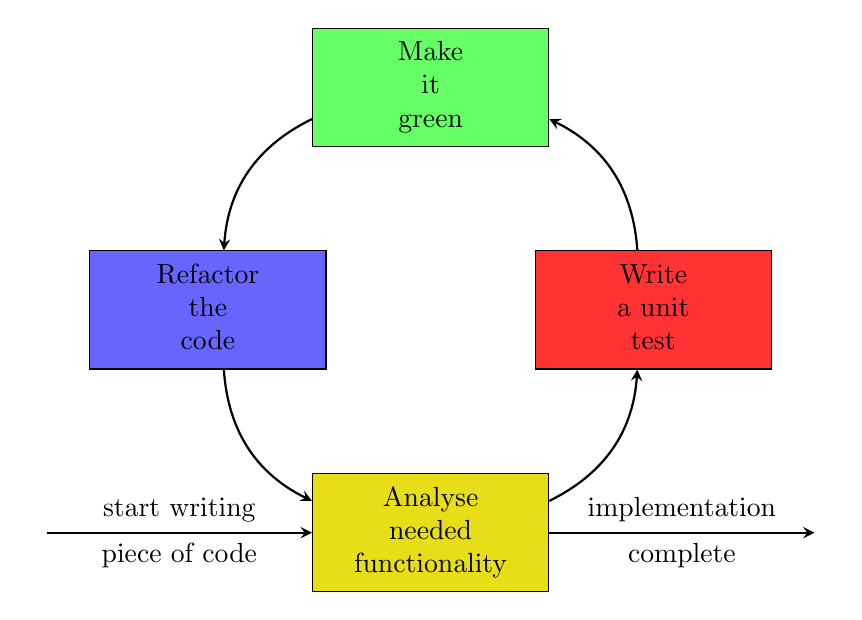
\begin{tikzpicture}
\node[rectangle, draw, fill = red!80, minimum width = 3cm](0){\begin{tabular}{c} Write \\ a unit \\ test\end{tabular}};
\node[rectangle, draw, fill = green!60, above left of = 0, node distance = 4cm, minimum width = 3cm](1){\begin{tabular}{c} Make \\ it \\ green\end{tabular}};
\node[rectangle, draw, fill = blue!60, below left of = 1, node distance = 4cm, minimum width = 3cm](2){\begin{tabular}{c} Refactor \\ the \\ code\end{tabular}};
\node[rectangle, draw, fill = yellow!90!black, below right of = 2, node distance = 4cm, minimum width = 3cm](3){\begin{tabular}{c} Analyse \\ needed \\ functionality\end{tabular}};
\node[left of = 3, node distance = 5cm](start){};
\node[right of = 3, node distance = 5cm](end){};

\draw[-stealth, thick]
(0) edge[bend right] (1)
(1) edge[bend right] (2)
(2) edge[bend right] (3)
(3) edge[bend right] (0)
(start) edge node[above]{start writing} node[below]{piece of code} (3)
(3) edge node[above]{implementation} node[below]{complete} (end)
;
\end{tikzpicture}
\end{frame}


\subsection*{Advantages and Disadvantages}

\begin{frame}{Advantages of Test-Driven Development}
\begin{itemize}	
	\item Developer thinks in an abstract way about all cases that can exist in the code
	\item Developer directly get feedback on correctness
	\item Systems written using TDD are easily testable
	\item Developers not demotivated by writing tests in the end
	\item Less problems if developer writes tests and code
	\item Using TDD for unit and system tests results in a metric representing the progress during implementation
	\item Using Becks method results in better code style due to the refactoring phase
	\item In general TDD results in a more modular code and easier extendable programs
\end{itemize}
\end{frame}

\begin{frame}{Concerns of Test-Driven Development}
\begin{itemize}
	\item Main argument against TDD is the high effort. But many people say this is not the case because
	\begin{itemize}
		\item After writing the tests, implementing is faster
		\item The developer directly gets feedback about correctness which results in less errors later
	\end{itemize}
	\item Studies were not able to show that less errors exist in written code thanks to using TDD
\end{itemize}
\end{frame}


\section{White-Box Testing}

\begin{Frame}{Path Coverage}
  \begin{itemize}
    \item Hope: reveal errors by executing paths of the program\\
    (independently of the values that variables take along the path).
    \item Ultimate white-box test is execution of every path in the program.\\
    (Unfeasible for general programs with loops.)
    \item Paths are partitioned into \alert{equivalence classes}, and test cases are designed trying to execute an element of each class.
  \end{itemize}

  \xxx

  \begin{definition}[Coverage]
    The \alert{(degree of) coverage} is the fraction of equivalence classes covered by the tests.
  \end{definition}
\end{Frame}

\newcommand{\resetpathstyle}{
  \tikzset{
    alphastyle/.style={},
    betastyle/.style={},
    gammastyle/.style={},
    deltastyle/.style={},
    epsilonstyle/.style={},
  }
  \let\alphabold\relax
  \let\betabold\relax
  \let\gammabold\relax
  \let\deltabold\relax
  \let\epsilonbold\relax
  \def\alphasymbol{$\alphabold\alpha$}
  \def\betasymbol{$\betabold\beta$}
  \def\gammasymbol{$\gammabold\gamma$}
  \def\deltasymbol{$\deltabold\delta$}
  \def\epsilonsymbol{$\epsilonbold\epsilon$}
}
\resetpathstyle

\newcommand<>{\alertpath}[3]{\only#4{
  \resetpathstyle
  \expandafter\def\csname #1bold\endcsname{\boldsymbol}
  \expandafter\def\csname #2bold\endcsname{\boldsymbol}
  \expandafter\def\csname #3bold\endcsname{\boldsymbol}
  \tikzset{
    #1style/.style={
      font=\bfseries,
      alertedcolor,
      thick
    },
    #2style/.style={
      font=\bfseries,
      alertedcolor,
      thick
    },
    #3style/.style={
      font=\bfseries,
      alertedcolor,
      thick
    }
  }
  \begin{tikzpicture}[
      stmt/.style={
        state,
        rectangle,
        minimum height=4ex,
        minimum width=6em
      },
      cond/.style={
        state,
        diamond,
        shape aspect=1.5,
        inner sep=0pt
      },
      on grid,
      node distance=.8cm and 2.5cm,
      shorten >=2pt,
      shorten <=2pt
    ]
    \node[coordinate] (init) {};
    \node[cond, below=of init] (cond1) {\shortstack{$a>1 \wedge {}$\\$b = 0$}};
    \node[stmt,below right=of cond1] (stmt1) {$x:=x/a$};
    \node[coordinate,below left=of stmt1] (join1) {};
    \node[cond,below=of join1] (cond2) {\shortstack{$a=2 \vee {}$\\$x > 1$}};
    \node[stmt,below right=of cond2] (stmt2) {$x := x + 1$};
    \node[coordinate,below left=of stmt2] (join2) {};
    \node[coordinate,below=of join2] (final) {};
    \path[thick, ->]
      (init) edge[alphastyle] node[left] {\alphasymbol} (cond1)
      (cond1) edge[betastyle] node[very near start, right] {no} node[left] {\betasymbol} (join1)
      (join1) edge[alphastyle] (cond2)
      (cond2) edge[deltastyle] node[very near start, right] {no} node[left] {\deltasymbol} (join2)
      (join2) edge[alphastyle] (final);
    \draw[thick, ->, gammastyle]
      (cond1) -| node[above,very near start] {yes} node[right] {\gammasymbol} (stmt1);
    \draw[thick, ->, gammastyle]
      (stmt1) |- (join1);
    \draw[thick, ->, epsilonstyle]
      (cond2) -| node[above,very near start] {yes} node[right] {\epsilonsymbol} (stmt2);
    \draw[thick, ->, epsilonstyle]
      (stmt2) |- (join2);
  \end{tikzpicture}
}}

\begin{Frame}{Running Example}
  \begin{center}
    \alertpath<1>{foo}{bar}{baz}
  \end{center}
\end{Frame}

\subsection{Control-flow-based Coverage}

\begin{Frame}{Statement Coverage}
  \begin{itemize}
    \item Choose test cases so that every \alert{statement} of the program is executed at least once.
    \item (Partitioning: all paths that visit an statement build an equivalence class.)
    \item Rationale: statement coverage catches all errors due to \enquote{catastrophic} statements
    \item \alert{Poor criterion}: we may never exercise one of the outcomes of a guard in if-then-else or loop constructs.
  \end{itemize}
\end{Frame}

\begin{Frame}{Statement Coverage}{Running Example}
  \begin{columns}
    \column{.6\textwidth}
      \alertpath<1>{alpha}{gamma}{epsilon}
    \column{.33\textwidth}
		\begin{center}
	     \begin{zebratabular}{ll}
	       \headerrow $(a,b,x)$ & path \\
	       \alert<1>{$(2, 0, 3)$} & \alert<1>{$\alpha\gamma\epsilon$} \\
	    \end{zebratabular}
		\end{center}
  \end{columns}
\end{Frame}

\begin{Frame}{Decision or Branch Coverage}
  \begin{itemize} 
    \item Choose test cases so that every possible outcome of each decision in the flow-graph occurs at least once.
    \item \alert{Observe:} this does not imply statement coverage (no decisions).
    \item Better formulation would be: every edge of the flow-graph is covered.
    \item \alert{Problem}: in a composite guard we may be setting an atom to the same truth value in all test cases.
  \end{itemize}
\end{Frame}

\begin{Frame}[fragile]{Decision or Branch Coverage}{Running Example}
  \begin{columns}
    \column{.6\textwidth}
      \alertpath<1>{alpha}{gamma}{delta}%
      \only<article>{\hfil\penalty0\hfilneg\quad}%
      \alertpath<2>{alpha}{beta}{epsilon}%
      \only<article>{\par\vskip3ex\par}%
      \alertpath<3>{alpha}{gamma}{epsilon}%
      \only<article>{\hfil\penalty0\hfilneg\quad}%
      \alertpath<4>{alpha}{beta}{delta}%
      \only<article>{\par\vskip3ex\par}%
    \column{.33\textwidth}
      \begin{center}
        \begin{zebratabular}{ll}
          \headerrow $(a,b,x)$ & path \\
          \alert<1>{$(3, 0, 3)$} & \alert<1>{$\alpha\gamma\delta$} \setrownumber1 \\
          \alert<2>{$(2, 1, 1)$} & \alert<2>{$\alpha\beta\epsilon$} \\
        \end{zebratabular}
        \mbox{}\vspace*{2ex}
        \begin{tabular}{l}
            Alternatively:
        \end{tabular}
        \begin{zebratabular}{ll}
          \headerrow $(a,b,x)$ & path \\
          \alert<3>{$(2, 0, 3)$} & \alert<3>{$\alpha\gamma\epsilon$} \setrownumber1 \\
          \alert<4>{$(3, 1, 1)$} & \alert<4>{$\alpha\beta\delta$} \\
        \end{zebratabular}
      \end{center}
  \end{columns}
\end{Frame}

\begin{Frame}{Condition coverage}
  \begin{itemize}
    \item Choose test cases so that every atom of each guard of the program is set to both \alert{true} and \alert{false} at least once (if at all possible)
    \item \alert{Observe}: condition coverage \alert{does not imply} decision
    coverage
    \item \alert{Observe}: can still be considered as path partitioning if 
    the evaluation of atoms is assumed to follow some order (refined flow-graph)
  \end{itemize}
\end{Frame}

\begin{Frame}{Condition coverage}{Running Example}
    \only<article>{
	    \begin{minipage}{.6\textwidth}
	      \alertpath<1>{alpha}{gamma}{epsilon}%
	    \end{minipage}\hfill
	    \begin{minipage}{.4\textwidth}
		    four conditions:\\
	        \ \ -- $a>1$, \goodmark\\
	        \ \ -- $b=0$, \goodmark\\
	        \ \ -- $a=2$, \goodmark\\
	        \ \ -- $x>1$\hphantom{,} \goodmark
	     
	     \vspace{2ex} 
       \begin{zebratabular}{ll}
         \headerrow $(a,b,x)$ & path \\
         \textcolor{alertedcolor}{$(2, 0, 3)$} & \textcolor{alertedcolor}{$\alpha\gamma\epsilon$} \setrownumber1 \\
         $(1, 1, 1)$ & $\alpha\beta\delta$ \\
       \end{zebratabular}  
	    \end{minipage}
	    
		  \vspace{3ex}
	    \begin{minipage}{.6\textwidth}
	      \alertpath<1>{alpha}{beta}{delta}%
	    \end{minipage}\hfill
	    \begin{minipage}{.4\textwidth}
		    four conditions:\\
	        \ \ -- $a>1$, \badmark\\
	        \ \ -- $b=0$, \badmark\\
	        \ \ -- $a=2$, \badmark\\
	        \ \ -- $x>1$\hphantom{,} \badmark
	        	     
 	     \vspace{2ex} 
        \begin{zebratabular}{ll}
          \headerrow $(a,b,x)$ & path \\
          $(2, 0, 3)$ & $\alpha\gamma\epsilon$ \setrownumber1 \\
          \textcolor{alertedcolor}{$(1, 1, 1)$} & \textcolor{alertedcolor}{$\alpha\beta\delta$} \\
        \end{zebratabular}
	    \end{minipage}
	    
	  \vspace{3ex}
 	    \begin{minipage}{.6\textwidth}
 	      \alertpath<1>{alpha}{beta}{epsilon}%
 	    \end{minipage}\hfill
 	    \begin{minipage}{.4\textwidth}
	 	    Alternatively:\\
 		    four conditions:\\
 	        \ \ -- $a>1$, \badmark\\
 	        \ \ -- $b=0$, \goodmark\\
 	        \ \ -- $a=2$, \badmark\\
 	        \ \ -- $x>1$\hphantom{,} \goodmark
 	        
 	      \vspace{2ex} 
        \begin{zebratabular}{ll}
          \headerrow $(a,b,x)$ & path \\
          \textcolor{alertedcolor}{$(1, 0, 3)$} & \textcolor{alertedcolor}{$\alpha\beta\epsilon$} \setrownumber2 \\
          $(2, 1, 1)$ & $\alpha\beta\epsilon$ \\
        \end{zebratabular} 	        
 	    \end{minipage}
 	    
	  \vspace{3ex}
 	    \begin{minipage}{.6\textwidth}
 	      \alertpath<1>{alpha}{beta}{epsilon}%
 	    \end{minipage}\hfill
 	    \begin{minipage}{.4\textwidth}
	 	    Alternatively:\\
 		    four conditions:\\
 	        \ \ -- $a>1$, \goodmark\\
 	        \ \ -- $b=0$, \badmark\\
 	        \ \ -- $a=2$, \goodmark\\
 	        \ \ -- $x>1$\hphantom{,} \badmark
 	     
 	      \vspace{2ex} 
        \begin{zebratabular}{ll}
          \headerrow $(a,b,x)$ & path \\
          $(1, 0, 3)$ & $\alpha\beta\epsilon$ \setrownumber2 \\
          \textcolor{alertedcolor}{$(2, 1, 1)$} & \textcolor{alertedcolor}{$\alpha\beta\epsilon$} \\
        \end{zebratabular}
 	    \end{minipage}
 	  }
	  \only<presentation>{
	  \begin{columns}
     \column{.6\textwidth}
     \alertpath<1>{alpha}{gamma}{epsilon}%
	   \alertpath<2>{alpha}{beta}{delta}%
     \alertpath<3-4>{alpha}{beta}{epsilon}%
     
     \column{.33\textwidth}
    
    \only<3,4>{Alternatively:\\}
    four conditions:\\
      \ \ -- $a>1$, \only<1,4>{\goodmark}\only<2,3>{\badmark}\\
      \ \ -- $b=0$, \only<1,3>{\goodmark}\only<2,4>{\badmark}\\
      \ \ -- $a=2$, \only<1,4>{\goodmark}\only<2,3>{\badmark}\\
      \ \ -- $x>1$\hphantom{,} \only<1,3>{\goodmark}\only<2,4>{\badmark}
		
		\xxx
		\only<1,2>{
	  \begin{zebratabular}{ll}
      \headerrow $(a,b,x)$ & path \\
      \alert<1>{$(2, 0, 3)$} & \alert<1>{$\alpha\gamma\epsilon$} \setrownumber1 \\
      \alert<2>{$(1, 1, 1)$} & \alert<2>{$\alpha\beta\delta$} \\
    \end{zebratabular}
    }
    \only<3,4>{
	  \begin{zebratabular}{ll}
      \headerrow $(a,b,x)$ & path \\
      \alert<3>{$(1, 0, 3)$} & \alert<3>{$\alpha\beta\epsilon$} \setrownumber1 \\
      \alert<4>{$(2, 1, 1)$} & \alert<4>{$\alpha\beta\epsilon$} \\
    \end{zebratabular}
    }
   \end{columns}
   }%
\end{Frame}

\begin{Frame}{Condition/Decision Coverage}
  \begin{itemize}
    \item Choose test cases so that every edge of the flow graph is executed at least once, and every atom of each guard of the program is set to both \alert{true} and \alert{false} at least once (if at all possible).
    \item \alert{Problem:} Some combinations of truth values for the atoms of a
    condition may not be tested $\rightarrow$ some edges of the refined flow-graph may not be covered.
  \end{itemize}
\end{Frame}

\begin{Frame}{Condition/Decision Coverage}{Running Example}
	\only<article>{
		\begin{minipage}{.6\textwidth}	
	    \alertpath<1>{alpha}{gamma}{epsilon}%
		\end{minipage}\hfill
		\begin{minipage}{.4\textwidth}
			four conditions:\\
      \ \ -- $a>1$, \goodmark\\
      \ \ -- $b=0$, \goodmark\\
      \ \ -- $a=2$, \goodmark\\
      \ \ -- $x>1$\hphantom{,} \goodmark
		
      \vspace{2ex}
		
      \begin{zebratabular}{ll}
        \headerrow $(a,b,x)$ & path \\
        \textcolor{alertedcolor}{$(2, 0, 3)$} & \textcolor{alertedcolor}{$\alpha\gamma\epsilon$} \setrownumber1 \\
        $(1, 1, 1)$ & $\alpha\beta\delta$ \\
      \end{zebratabular}
		\end{minipage}
		
		\vspace{3ex}
		
		\begin{minipage}{.6\textwidth}
			\alertpath<2>{alpha}{beta}{delta}%
		\end{minipage}\hfill
		\begin{minipage}{.4\textwidth}
			four conditions:\\
      \ \ -- $a>1$, \badmark\\
      \ \ -- $b=0$, \badmark\\
      \ \ -- $a=2$, \badmark\\
      \ \ -- $x>1$\hphantom{,} \badmark
		
      \vspace{2ex}
		
      \begin{zebratabular}{ll}
        \headerrow $(a,b,x)$ & path \\
        $(2, 0, 3)$ & $\alpha\gamma\epsilon$ \setrownumber1 \\
        \textcolor{alertedcolor}{$(1, 1, 1)$} & \textcolor{alertedcolor}{$\alpha\beta\delta$} \\
      \end{zebratabular}
		\end{minipage}	
	}


	\only<presentation>{
	  \begin{columns}
	    \column{.6\textwidth}
	      \alertpath<1>{alpha}{gamma}{epsilon}%
	      \alertpath<2>{alpha}{beta}{delta}%
	    \column{.33\textwidth}
	      four conditions:\\
	      \ \ -- $a>1$, \only<1>{\goodmark}\only<2>{\badmark}\\
	      \ \ -- $b=0$, \only<1>{\goodmark}\only<2>{\badmark}\\
	      \ \ -- $a=2$, \only<1>{\goodmark}\only<2>{\badmark}\\
	      \ \ -- $x>1$\hphantom{,} \only<1>{\goodmark}\only<2>{\badmark}
	
	      \xxx
	
	      \begin{zebratabular}{ll}
	        \headerrow $(a,b,x)$ & path \\
	        \alert<1>{$(2, 0, 3)$} & \alert<1>{$\alpha\gamma\epsilon$} \setrownumber1 \\
	        \alert<2>{$(1, 1, 1)$} & \alert<2>{$\alpha\beta\delta$} \\
	      \end{zebratabular}
	  \end{columns}
  }
\end{Frame}

\begin{Frame}{Multiple Condition Coverage}
  \begin{itemize}
    \item Choose test cases so that for each guard every possible combination of truth values of the atoms occurs at least once.
    \item \alert{Problem}: for a boolean guard with $n$ atoms there are $2^n$
    possible combinations.
    \item Multiple condition coverage implies decision/condition coverage.
    \item \alert{Observe}: multiple condition coverage \alert{does not} imply coverage of all possible paths. ($\alpha\gamma\delta$ is not covered in next example.)
  \end{itemize}
\end{Frame}

\begin{Frame}{Multiple Condition Coverage}{Running Example}

	\only<article>{
		\begin{minipage}{.6\textwidth}
	     \alertpath<1>{alpha}{gamma}{epsilon}%
		\end{minipage}\hfill
		\begin{minipage}{.4\textwidth}
		   four conditions:\\
		   \ \ -- $a>1$, \goodmark\\
		   \ \ -- $b=0$, \goodmark\\
		   \ \ -- $a=2$, \goodmark\\
		   \ \ -- $x>1$\hphantom{,} \goodmark
		
		   \vspace{2ex}
		
		   \begin{zebratabular}{ll}
		     \headerrow $(a,b,x)$ & path \\
		     \textcolor{alertedcolor}{$(2, 0, 4)$} & \textcolor{alertedcolor}{$\alpha\gamma\epsilon$} \setrownumber1 \\
		     $(2, 1, 1)$ & $\alpha\beta\epsilon$ \setrownumber1 \\
		     $(1, 0, 2)$ & $\alpha\beta\epsilon$ \setrownumber1 \\
		     $(1, 1, 1)$ & $\alpha\beta\delta$ \setrownumber1 \\
		   \end{zebratabular}	
		\end{minipage}
		
		\vspace{3ex}

		\begin{minipage}{.6\textwidth}
			\alertpath<2>{alpha}{beta}{epsilon}%
		\end{minipage}\hfill
		\begin{minipage}{.4\textwidth}
		   four conditions:\\
		   \ \ -- $a>1$, \goodmark\\
		   \ \ -- $b=0$, \badmark\\
		   \ \ -- $a=2$, \goodmark\\
		   \ \ -- $x>1$\hphantom{,} \badmark
				
		   \vspace{2ex}
				
		   \begin{zebratabular}{ll}
		     \headerrow $(a,b,x)$ & path \\
		     $(2, 0, 4)$ & $\alpha\gamma\epsilon$ \setrownumber1 \\
		     \textcolor{alertedcolor}{$(2, 1, 1)$} & \textcolor{alertedcolor}{$\alpha\beta\epsilon$} \setrownumber1 \\
		     $(1, 0, 2)$ & $\alpha\beta\epsilon$ \setrownumber1 \\
		     $(1, 1, 1)$ & $\alpha\beta\delta$ \setrownumber1 \\
		   \end{zebratabular}		
		\end{minipage}
		
		\vspace{3ex}

		\begin{minipage}{.6\textwidth}
	    \alertpath<3>{alpha}{beta}{epsilon}%
		\end{minipage}\hfill
		\begin{minipage}{.4\textwidth}
		  four conditions:\\
		  \ \ -- $a>1$, \badmark\\
		  \ \ -- $b=0$, \goodmark\\
		  \ \ -- $a=2$, \badmark\\
		  \ \ -- $x>1$\hphantom{,} \goodmark
						
		  \vspace{2ex}
						
		  \begin{zebratabular}{ll}
		    \headerrow $(a,b,x)$ & path \\
		    $(2, 0, 4)$ & $\alpha\gamma\epsilon$ \setrownumber1 \\
		    $(2, 1, 1)$ & $\alpha\beta\epsilon$ \setrownumber1 \\
		    \textcolor{alertedcolor}{$(1, 0, 2)$} & \textcolor{alertedcolor}{$\alpha\beta\epsilon$} \setrownumber1 \\
		    $(1, 1, 1)$ & $\alpha\beta\delta$ \setrownumber1 \\
		  \end{zebratabular}		
		\end{minipage}
		
		\vspace{3ex}

		\begin{minipage}{.6\textwidth}
	    \alertpath<4>{alpha}{beta}{delta}%				
		\end{minipage}\hfill
		\begin{minipage}{.4\textwidth}
		  four conditions:\\
		  \ \ -- $a>1$, \badmark\\
		  \ \ -- $b=0$, \badmark\\
		  \ \ -- $a=2$, \badmark\\
		  \ \ -- $x>1$\hphantom{,} \badmark
								
		  \vspace{2ex}
								
		  \begin{zebratabular}{ll}
		    \headerrow $(a,b,x)$ & path \\
		    $(2, 0, 4)$ & $\alpha\gamma\epsilon$ \setrownumber1 \\
		    $(2, 1, 1)$ & $\alpha\beta\epsilon$ \setrownumber1 \\
		    $(1, 0, 2)$ & $\alpha\beta\epsilon$ \setrownumber1 \\
		    \textcolor{alertedcolor}{$(1, 1, 1)$} & \textcolor{alertedcolor}{$\alpha\beta\delta$} \setrownumber1 \\
		  \end{zebratabular}			
		\end{minipage}		
	}

	\only<presentation>{
	  \begin{columns}
	    \column{.6\textwidth}
	      \alertpath<1>{alpha}{gamma}{epsilon}%
	      \alertpath<2>{alpha}{beta}{epsilon}%
	      \alertpath<3>{alpha}{beta}{epsilon}%
	      \alertpath<4>{alpha}{beta}{delta}%
	    \column{.33\textwidth}
	      four conditions:\\
	      \ \ -- $a>1$, \only<1,2>{\goodmark}\only<3,4>{\badmark}\\
	      \ \ -- $b=0$, \only<1,3>{\goodmark}\only<2,4>{\badmark}\\
	      \ \ -- $a=2$, \only<1,2>{\goodmark}\only<3,4>{\badmark}\\
	      \ \ -- $x>1$\hphantom{,} \only<1,3>{\goodmark}\only<2,4>{\badmark}
	
	      \xxx
	
	      \begin{zebratabular}{ll}
	        \headerrow $(a,b,x)$ & path \\
	        \alert<1>{$(2, 0, 4)$} & \alert<1>{$\alpha\gamma\epsilon$} \setrownumber1 \\
	        \alert<2>{$(2, 1, 1)$} & \alert<2>{$\alpha\beta\epsilon$} \setrownumber1 \\
	        \alert<3>{$(1, 0, 2)$} & \alert<3>{$\alpha\beta\epsilon$} \setrownumber1 \\
	        \alert<4>{$(1, 1, 1)$} & \alert<4>{$\alpha\beta\delta$} \setrownumber1 \\
	      \end{zebratabular}
	  \end{columns}
  }
\end{Frame}


\begin{Frame}{Modified Condition/Decision Coverage}
  \begin{itemize}
  	\item MC/DC is the most complex criterion used in the industry (mainly avionics).
  	\item More feasible than MCC because $n+1$ minimum test cases, not $2^n$.

    \item Every atom of each guard of the program is set to both true and false at least once, such that
    \begin{itemize}
      \item each atom independently affects the outcome of the guard (if possible).
    \end{itemize}
  \end{itemize}
	
  
\end{Frame}


\begin{Frame}{Modified Condition/Decision Coverage}

How to show the independent effect:
	\begin{itemize}
		\item Find two test cases where only one condition and the outcome of the decision changes.
		\item Hold all other conditions fixed (if possible).
	\end{itemize}
\end{Frame}



\begin{Frame}{Modified Condition/Decision Coverage}{Running Example: Influences on the first guard}
  \only<article>{
    \begin{minipage}{.6\textwidth}
      \alertpath<1>{foo}{bar}{baz}%
      \alertpath<2>{foo}{bar}{baz}%
      \alertpath<3>{foo}{bar}{baz}%
      \alertpath<4>{foo}{bar}{baz}%
    \end{minipage}\hfill
    \begin{minipage}{.4\textwidth}
      Influence of $a$ on the first guard\\[1ex]
      \begin{zebratabular}{ll}
        \headerrow $(a,b)$ & guard \\
        \alert<1>{$(2, 0)$} & true \\
        \alert<2>{$(0, 0)$} & false\\
      \end{zebratabular}
      \par\vspace{2ex}
      Influence of $b$ on the first guard\\[1ex]
      \begin{zebratabular}{ll}
        \headerrow $(a,b)$ & guard \\
        \alert<3>{$(2, 0)$} & true \\
        \alert<4>{$(2, 1)$} & false\\
      \end{zebratabular}
    \end{minipage}
  }
  \only<presentation>{  
    \begin{columns}
      \column{.6\textwidth}
        \alertpath<1>{gamma}{none}{none}
        \alertpath<2>{beta}{none}{none}
        \alertpath<3>{gamma}{none}{none}
        \alertpath<4>{beta}{none}{none}
      \column{.33\textwidth}
        Influence of $a$ on the first guard\\[1ex]
        \begin{zebratabular}{ll}
          \headerrow $(a,b,x)$ & guard \\
          \alert<1>{$(2, 0, -)$} & true \\
          \alert<2>{$(1, 0, -)$} & false\\
        \end{zebratabular}
        \par\vspace{2ex}
        Influence of $b$ on the first guard\\[1ex]
        \begin{zebratabular}{ll}
          \headerrow $(a,b,x)$ & guard \\
          \alert<3>{$(2, 0, -)$} & true \\
          \alert<4>{$(2, 1, -)$} & false\\
        \end{zebratabular}
    \end{columns}}
\end{Frame}


\begin{frame}{Modified Condition/Decision Coverage}{Running Example: Influences on the second guard}
  \only<article>{
    \begin{minipage}{.6\textwidth}
       \alertpath<1>{epsilon}{none}{none}%
       \alertpath<2>{delta}{none}{none}%
       \alertpath<3>{epsilon}{none}{none}%
       \alertpath<4>{delta}{none}{none}%
    \end{minipage}\hfill
    \begin{minipage}{.4\textwidth}
      Influence of $a$ on the second guard\\[1ex]
      \begin{zebratabular}{ll}
        \headerrow $(a,b,x)$ & guard \\
        \alert<1>{$(2, -, 2)$} & true \\
        \alert<2>{$(1, -, 2)$} & false\\
      \end{zebratabular}
      \par\vspace{2ex}
      Influence of $x$ on the second guard\\[1ex]
      \begin{zebratabular}{ll}
        \headerrow $(a,b,x)$ & guard \\
        \alert<3>{$(1, -, 2)$} & true \\
        \alert<4>{$(1, -, 0)$} & false\\
      \end{zebratabular}
    \end{minipage}
  }
  \only<presentation>{  
    \begin{columns}
      \column{.6\textwidth}
        \alertpath<1>{epsilon}{none}{none}
        \alertpath<2>{delta}{none}{none}
        \alertpath<3>{epsilon}{none}{none}
        \alertpath<4>{delta}{none}{none}
      \column{.33\textwidth} 
        Influence of $a$ on the second guard\\[1ex]
        \begin{zebratabular}{ll}
          \headerrow $(a,b,x)$ & guard \\
          \alert<1>{$(2, -, 2)$} & true \\
          \alert<2>{$(1, -, 2)$} & false\\
        \end{zebratabular}
        \par\vspace{2ex}
        Influence of $x$ on the second guard\\[1ex]
        \begin{zebratabular}{ll}
          \headerrow $(a,b,x)$ & guard \\
          \alert<3>{$(1, -, 2)$} & true \\
          \alert<4>{$(1, -, 0)$} & false\\
        \end{zebratabular}
    \end{columns}}
\end{frame}


\begin{frame}{Modified Condition/Decision Coverage}{Running Example: Final Test Suite}

	\only<article>{
		\begin{minipage}{.6\textwidth}
	     \alertpath<1>{alpha}{gamma}{epsilon}%
		\end{minipage}\hfill
		\begin{minipage}{.4\textwidth}
		     Final Test Suite\\
		   		  \begin{zebratabular}{ll}
		          \headerrow $(a,b,x)$ & path \\
		          \textcolor{alertedcolor}{$(2, 0, 1)$} & \textcolor{alertedcolor}{$\alpha\gamma\epsilon$} \setrownumber1 \\
		          $(1, 0, 1)$ & $\alpha\beta\delta$ \setrownumber1 \\
		          $(2, 1, 2)$ & $\alpha\beta\epsilon$ \setrownumber1 \\
		          $(1, 1, 2)$ & $\alpha\beta\epsilon$ \setrownumber1 \\
		          $(1, 1, 0)$ & $\alpha\beta\delta$ \setrownumber1 \\
		        \end{zebratabular}
		\end{minipage}
		
		\vspace{3ex}

		\begin{minipage}{.6\textwidth}
			\alertpath<2>{alpha}{beta}{delta}%
		\end{minipage}\hfill
		\begin{minipage}{.4\textwidth}
		  Final Test Suite\\
				  \begin{zebratabular}{ll}
		       \headerrow $(a,b,x)$ & path \\
		       $(2, 0, 1)$ & $\alpha\gamma\epsilon$ \setrownumber1 \\
		       \textcolor{alertedcolor}{$(1, 0, 1)$} & \textcolor{alertedcolor}{$\alpha\beta\delta$} \setrownumber1 \\
		       $(2, 1, 2)$ & $\alpha\beta\epsilon$ \setrownumber1 \\
		       $(1, 1, 2)$ & $\alpha\beta\epsilon$ \setrownumber1 \\
		       $(1, 1, 0)$ & $\alpha\beta\delta$ \setrownumber1 \\
		     \end{zebratabular}
		\end{minipage}
		
		\vspace{3ex}

		\begin{minipage}{.6\textwidth}
	    \alertpath<3>{alpha}{beta}{epsilon}%
		\end{minipage}\hfill
		\begin{minipage}{.4\textwidth}
	  Final Test Suite\\
			  \begin{zebratabular}{ll}
	       \headerrow $(a,b,x)$ & path \\
	       $(2, 0, 1)$ & $\alpha\gamma\epsilon$ \setrownumber1 \\
	       $(1, 0, 1)$ & $\alpha\beta\delta$ \setrownumber1 \\
	       \textcolor{alertedcolor}{$(2, 1, 2)$} & \textcolor{alertedcolor}{$\alpha\beta\epsilon$} \setrownumber1 \\
	       $(1, 1, 2)$ & $\alpha\beta\epsilon$ \setrownumber1 \\
	       $(1, 1, 0)$ & $\alpha\beta\delta$ \setrownumber1 \\
	     \end{zebratabular}
		\end{minipage}
		
		\vspace{3ex}

		\begin{minipage}{.6\textwidth}
	    \alertpath<4>{alpha}{beta}{epsilon}%				
		\end{minipage}\hfill
		\begin{minipage}{.4\textwidth}
		   Final Test Suite\\
				  \begin{zebratabular}{ll}
		       \headerrow $(a,b,x)$ & path \\
		       $(2, 0, 1)$ & $\alpha\gamma\epsilon$ \setrownumber1 \\
		       $(1, 0, 1)$ & $\alpha\beta\delta$ \setrownumber1 \\
		       $(2, 1, 2)$ & $\alpha\beta\epsilon$ \setrownumber1 \\
		       \textcolor{alertedcolor}{$(1, 1, 2)$} & \textcolor{alertedcolor}{$\alpha\beta\epsilon$} \setrownumber1 \\
		       $(1, 1, 0)$ & $\alpha\beta\delta$ \setrownumber1 \\
		     \end{zebratabular}
		\end{minipage}		
		
		\vspace{3ex}

		\begin{minipage}{.6\textwidth}
		  \alertpath<5>{alpha}{beta}{delta}%		
		\end{minipage}\hfill
		\begin{minipage}{.4\textwidth}
		   Final Test Suite\\
				  \begin{zebratabular}{ll}
		       \headerrow $(a,b,x)$ & path \\
		       $(2, 0, 1)$ & $\alpha\gamma\epsilon$ \setrownumber1 \\
		       $(1, 0, 1)$ & $\alpha\beta\delta$ \setrownumber1 \\
		       $(2, 1, 2)$ & $\alpha\beta\epsilon$ \setrownumber1 \\
		       $(1, 1, 2)$ & $\alpha\beta\epsilon$ \setrownumber1 \\
		       \textcolor{alertedcolor}{$(1, 1, 0)$} & \textcolor{alertedcolor}{$\alpha\beta\delta$} \setrownumber1 \\
		     \end{zebratabular}
		\end{minipage}
		\mbox{}	
}%

	\only<presentation>{
	  \begin{columns}
	    \column{.6\textwidth}
	      \alertpath<1>{alpha}{gamma}{epsilon}%
   			\alertpath<2>{alpha}{beta}{delta}%
		    \alertpath<3>{alpha}{beta}{epsilon}%
   	    \alertpath<4>{alpha}{beta}{epsilon}%	
    	  \alertpath<5>{alpha}{beta}{delta}%				
	    \column{.33\textwidth}
	      Final Test Suite\\[1ex]
	      \begin{zebratabular}{ll}
		       \headerrow $(a,b,x)$ & path \\
		       \alert<1>{$(2, 0, 1)$} & \alert<1>{$\alpha\gamma\epsilon$} \setrownumber1 \\
		       \alert<2>{$(1, 0, 1)$} & \alert<2>{$\alpha\beta\delta$} \setrownumber1 \\
		       \alert<3>{$(2, 1, 2)$} & \alert<3>{$\alpha\beta\epsilon$} \setrownumber1 \\
		       \alert<4>{$(1, 1, 2)$} & \alert<4>{$\alpha\beta\epsilon$} \setrownumber1 \\
		       \alert<5>{$(1, 1, 0)$} & \alert<5>{$\alpha\beta\delta$} \setrownumber1 \\
	      \end{zebratabular}
	  \end{columns}
  }
\end{frame}



\subsection{Data-flow-based Coverage}

\begin{frame}{Data-flow-based Coverage}
  $\forall x$ we define \alert{sets of nodes} of the flowchart:
  \begin{description}
    \item[def($x$)] nodes where some value is assigned to $x$ ($x$ is {\textit defined})
    \item[p-use($x$)] nodes where $x$ is used in a guard (also called a {\em predicate})
    \item[c-use($x$)] nodes where $x$ is used in some expression other than a predicate (also called a \alert{command}, typically the right-hand-side of an assignment).\hfill\vspace{3ex}\linebreak
    \item[def-clear($x$)] is the \alert{set of paths} of the flowchart that:
  \end{description}
  \vskip-1ex
  \begin{itemize}\setbeamertemplate{itemize item}{--}
    \item contain each node at most once, except for the first and last nodes,
    which may be the same;\\
    \item do not contain any node of def($x$), except for possibly the first node (and the last node, if it coincides with the first).
  \end{itemize}
\end{frame}

\newcommand{\resetlabeledpathstyle}{
  \tikzset{
    alphastyle/.style={},
    betastyle/.style={},
    gammastyle/.style={},
    deltastyle/.style={},
    epsilonstyle/.style={},
    betatwostyle/.style={},
    gammatwostyle/.style={},
    deltatwostyle/.style={},
    epsilontwostyle/.style={}
  }
  \let\alphabold\relax
  \let\betabold\relax
  \let\gammabold\relax
  \let\deltabold\relax
  \let\epsilonbold\relax
  \def\alphasymbol{$\alphabold\alpha$}
  \def\betasymbol{$\betabold\beta$}
  \def\gammasymbol{$\gammabold\gamma$}
  \def\deltasymbol{$\deltabold\delta$}
  \def\epsilonsymbol{$\epsilonbold\epsilon$}
}
\resetlabeledpathstyle

\newcommand<>{\alertlabeledpath}[7]{\only#8{
  \resetlabeledpathstyle
  \expandafter\def\csname #1bold\endcsname{\boldsymbol}
  \expandafter\def\csname #2bold\endcsname{\boldsymbol}
  \expandafter\def\csname #3bold\endcsname{\boldsymbol}
  \tikzset{
    #1style/.style={
      font=\bfseries,
      alertedcolor,
      thick
    },
    #2style/.style={
      font=\bfseries,
      alertedcolor,
      thick
    },
    #3style/.style={
      font=\bfseries,
      alertedcolor,
      thick
    },
    #4style/.style={
      font=\bfseries,
      alertedcolor,
      thick
    },
    #5style/.style={
      font=\bfseries,
      alertedcolor,
      thick
    },
    #6style/.style={
      font=\bfseries,
      alertedcolor,
      thick
    },
    #7style/.style={
      font=\bfseries,
      alertedcolor,
      thick
    }
  }
  \begin{tikzpicture}[
      stmt/.style={
        state,
        rectangle,
        minimum height=4ex,
        minimum width=6em,
        label=above 
        right:{\shortstack{\color{maincolor}\bfseries 
        c-use($x$)\\\color{maincolor}\bfseries def($x$)}}
      },
      cond/.style={
        state,
        diamond,
        shape aspect=1.5,
        inner sep=0pt
      },
      on grid,
      node distance=.8cm and 2.5cm,
      shorten >=2pt,
      shorten <=2pt
    ]
    \node[coordinate, label=above:$A$] (init) {};
    \node[cond, below=of init, label=above left:$B$] (cond1) {\shortstack{$a>1 \wedge {}$\\$b = 0$}};

    \node[stmt,below right=of cond1,label=right:$C$] (stmt1) {$x:=x/a$};

    \node[coordinate,below left=of stmt1] (join1) {};

    \node[cond,below=of join1,label=above right:{\textcolor{maincolor}{\bfseries p-use($x$)}},label=above left:$D$] (cond2) {\shortstack{$a=2 \vee {}$\\$x > 1$}};

    \node[stmt,below right=of cond2,label=right:$E$] (stmt2) {$x := x + 1$};

    \node[coordinate,below left=of stmt2] (join2) {};
    \node[coordinate,below=of join2] (final) {};

    \path[thick, ->]
      (init) edge[alphastyle] node[left] {\alphasymbol} (cond1)
      (cond1) edge[betastyle] node[very near start, right] {no} node[left] {\betasymbol} (join1)
      (join1) edge[betatwostyle] (cond2)
      (cond2) edge[deltastyle] node[very near start, right] {no} node[left] {\deltasymbol} (join2)
      (join2) edge[deltatwostyle] (final);
    \draw[thick, ->, gammastyle]
      (cond1) -| node[above,very near start] {yes} node[right] {\gammasymbol} (stmt1);
    \draw[thick, ->, gammatwostyle]
      (stmt1) |- (join1);
    \draw[thick, ->, epsilonstyle]
      (cond2) -| node[above,very near start] {yes} node[right] {\epsilonsymbol} (stmt2);
    \draw[thick, ->, epsilontwostyle]
      (stmt2) |- (join2);
  \end{tikzpicture}
}}






\begin{Frame}{Data-flow-based Coverage}{Running Example}
  \begin{columns}
    \column{.6\textwidth}
	    \alertlabeledpath<1>{alpha}{beta}{delta}{betatwo}{deltatwo}{foo}{bar}%
    \column{.33\textwidth}
	    \only<presentation>{
      \textcolor{maincolor}{\bfseries def-clear($x$)} $=$ \\
      \ \ $\{ \alpha, \alpha\beta, \alert{\alpha\beta\delta} \}$
      }
      \only<article>{
	      \begin{center}
		      \textcolor{maincolor}{\bfseries def-clear($x$)} $= \{ \alpha, \alpha\beta, \alert{\alpha\beta\delta} \}$
	      \end{center}
      }
  \end{columns}
\end{Frame}


\begin{Frame}{Data-flow-based Coverage: dpu and dcu}
  For each node $s$ and every variable $x$ we define the following sets of nodes:
  \begin{description}
    \item[dcu($s,x$)] the set of nodes $s' \in$ c-use($x$) such that there is a def-clear($x$) path from $s$ to $s'$
    \item[dpu($s,x$)] the set of nodes $s' \in$ p-use($x$) such that there is a def-clear($x$) path from $s$ to $s'$.
  \end{description}
\end{Frame}

\begin{Frame}{Data-flow-based Coverage: dpu and dcu}{Running Example}
	\only<presentation>{
	  \begin{columns}
	    \column{.6\textwidth}
	      \alertlabeledpath<1>{alpha}{gamma}{foo}{foo}{bar}{baz}{foo}%
	      \alertlabeledpath<2>{alpha}{beta}{betatwo}{epsilon}{bar}{baz}{foo}%
	      \alertlabeledpath<3>{alpha}{beta}{betatwo}{foo}{bar}{baz}{foo}%
	    \column{.33\textwidth}
	      \textcolor{maincolor}{\bfseries dcu($A$, $x$)} $=$ \\
	      \ \ $\{ \alert<1>{C}, \alert<2>{E} \}$\hfill\vspace{3ex}\linebreak
	
	      \textcolor{maincolor}{\bfseries dpu($A$, $x$)} $=$ \\
	      \ \ $\{ \alert<3>{D} \}$
	  \end{columns}
  }
  \only<article>{
	  \begin{minipage}{.6\textwidth}
		  \alertlabeledpath<1>{alpha}{gamma}{foo}{foo}{bar}{baz}{foo}%	
	  \end{minipage}\hfill
	  \begin{minipage}{.4\textwidth}
		  \textcolor{maincolor}{\bfseries dcu($A$, $x$)} $=\{ \textcolor{alertedcolor}{C}, E \}$\hfill\vspace{3ex}\linebreak
		  
			\textcolor{maincolor}{\bfseries dpu($A$, $x$)} $= \{ D \}$
	  \end{minipage}
	  
	  \vspace{3ex}
	  
	  \begin{minipage}{.6\textwidth}
	    \alertlabeledpath<1>{alpha}{beta}{betatwo}{epsilon}{bar}{baz}{foo}%	
	  \end{minipage}\hfill
	  \begin{minipage}{.4\textwidth}
		  \textcolor{maincolor}{\bfseries dcu($A$, $x$)} $=\{ C, \textcolor{alertedcolor}{E} \}$\hfill\vspace{3ex}\linebreak
		  
			\textcolor{maincolor}{\bfseries dpu($A$, $x$)} $= \{ D \}$
	  \end{minipage}
	  
	  \vspace{3ex}
	  
	  \begin{minipage}{.6\textwidth}
	    \alertlabeledpath<1>{alpha}{beta}{betatwo}{foo}{bar}{baz}{foo}%	
	  \end{minipage}\hfill
	  \begin{minipage}{.4\textwidth}
		  \textcolor{maincolor}{\bfseries dcu($A$, $x$)} $=\{ C, E \}$\hfill\vspace{3ex}\linebreak
		  
			\textcolor{maincolor}{\bfseries dpu($A$, $x$)} $= \{ \textcolor{alertedcolor}{D} \}$
	  \end{minipage}  
  }
\end{Frame}

\begin{Frame}{Data-flow Coverage Criteria}
  $\forall x$ and $\forall s \in$ def($x$), the set $R$ of paths realized by the suite contains \ldots\\
  \xxx
  \begin{description}
    \item[all-defs] one path to some node in dpu($s,x$) or dcu($s,x$).\\
    $\Rightarrow$ \textit{All defs are used somewhere.}
    \item[all-p-uses] one path to each node in dpu($s,x$).\\
    $\Rightarrow$ \textit{All branches affected by each definition are exercised.}
    %\item[all-p-uses/some-c-uses] one path to each node in dpu($s,x$), but if dpu($s,x$) is empty, then at least one path to some node in dcu($s,x$).\\
    %$\Rightarrow$ \textit{All definitions are used and if they affect control flow then all affected branches are exercised.}
      \end{description}
\end{Frame}

\begin{Frame}{Data-flow Coverage Criteria}
  \begin{description}
    %\item[all-c-uses/some-p-uses] one path to each node in dcu($s,x$), but if dcu($s,x$) is empty, then at least one path to some node in dpu($s,x$).\\
    %$\Rightarrow$ \textit{All definition are used and if they affect computations then all affected computation are exercised.}
    \item[all uses] one path to each node in dpu($s,x$) and to each node in dcu($s,x$).\\
	$\Rightarrow$ \textit{Every computation and branch directly affected by a definition is exercised.}
    \item[all-du-paths] all paths to each node in dpu($s,x$) and to each node in dcu($s,x$).\\
    $\Rightarrow$ \textit{Every computation and branch directly affected by a definition is exercised and all def-use paths are exercised.}
  \end{description}
\end{Frame}

\begin{Frame}{Data-flow Coverage Criteria}

	Data-flow Analysis can be useful to discover potential faults in the program.\\
	\xxx
	Examples:
	\begin{itemize}
		\item Is the definition of a variable that is not used in the program useful?
		\item Are we using a variable before it is defined? 
		\item Are some variables only used in certain parts of the program?
	\end{itemize}

\end{Frame}


\subsection{Mutation Testing}

\begin{frame}{Mutation Testing}
	Test Suite Evaluation: How good is my test-suite?
	\begin{beameritemize}
		\item (How) is every statement executed? ($\Rightarrow$ Coverage)
		\item Can my test cases detect faulty changes in the code?
	\end{beameritemize}	
	\xxx
	\begin{block}{Idea}
		Introduce small changes (mutations) to the code and see if a test case can detect it.
	\end{block}	
\end{frame}


\begin{frame}{Mutation Testing}
	
	
	Examples (Conditionals Boundary Mutations):\\
	\texttt{if(a<b)~} $\Rightarrow$ \texttt{if(a<=b)}\\
	\texttt{if(a==b)} $\Rightarrow$ \texttt{if(a!=b)}\\
	\texttt{if(a\&\&b)} $\Rightarrow$ \texttt{if(a||b)}\\
	\texttt{if(a\&\&b)} $\Rightarrow$ \texttt{if(a\&\&true)}\\	
	\xxx
	Examples (Math Mutations):\\
	\texttt{a+b} $\Rightarrow$ \texttt{a-b}\\
	\texttt{a*b} $\Rightarrow$ \texttt{a/b}\\
	\texttt{a\&b} $\Rightarrow$ \texttt{a|b}\\
	\texttt{a<<b} $\Rightarrow$ \texttt{a>>b}\\	
\end{frame}

\begin{frame}{Mutation Testing}
	\begin{block}{Mutation Detection}
		\begin{beameritemize}
			\item Compare the results of original an mutant program. 
			\item A mutation is considered detected or "killed", if at least one test case reaches the mutation and at least one test case recognized the change in the program.
			\item If all test cases produce the same result for the original and mutant program, a mutation is kept alive and a more effective test case has to be created.
			\item Typical metric: Mutation Score $=($Killed Mutants $/$ Total number of Mutants$)*100$
		\end{beameritemize}	
		
	\end{block}
	
\end{frame}


\begin{frame}{Mutation Testing}		
	
	\begin{tikzpicture}[scale=0.40]
	\node[state, initial, field] (source) {Source Code};
	\node[state, field, right=0.5cm of source] (mutation) {Mutation};
	\node[state, field, right=0.5cm of mutation] (mutated) {Mutated Source Code}; 
	\node[state, field, below=of mutated] (suite) {Test Suite};   
	\node[state, field, error , below =1cm of suite] (error) {All Tests Passed};
	\node[state, field, success, below left=1cm and 1cm of suite] (success) {Test Failed/Mutation killed};
	\node[state, field, error, below=of error] (bug) {Unsufficient Test Suite!};     
	
	
	\draw[->] (success.north) -| (source.south);
	
	
	\path[->]
	(source) edge node {} (mutation)
	(mutation) edge node {} (mutated)
	(mutated.south) edge node {} (suite.north)
	(suite.south) edge node {} (success.north)
	(suite.south) edge node {} (error.north)
	(error) edge node {} (bug)
	
	;
	
	\end{tikzpicture}
\end{frame}

\begin{frame}{Mutation Testing}
	Advantages:
	\begin{beameritemize}
		\item Can help to improve and validate the test suite.
		\item Better tests can find unknown bugs.
	\end{beameritemize}	
	\xxx
	Disadvantages:
	\begin{beameritemize}
		\item Each generated mutant has to be executed by the entire test suite.
		\item Extremely costly and time consuming.
	\end{beameritemize}
	\xxx
	$\Rightarrow$ Hands-on example in the exercises!	
\end{frame}


\subsection{Property-based Testing}

\begin{frame}{Automatic test case generation}
	How can I sufficiently test my code without writing hundreds of cases?
	\xxx
	\begin{block}{Idea}
		Automatically generate input values.
	\end{block}	

	$\Rightarrow$ Problem: How can we know the correct output, if the input is randomly generated?
\end{frame}



\begin{frame}{Property-based Testing}
	\begin{block}{Property-based Testing}
		Define properties and criteria for outputs that should be true for any arbitrary inputs.
		If the properties hold for big number of generated inputs, we assume that the code is correct.
	\end{block}	

		
\end{frame}

\begin{frame}{Property-based Testing}
	Example: Test a function that takes two numbers and returns the sum of them.
	\xxx
	\begin{block}{Exercise}
		Find three properties that are true for adding two numbers and that are not true for other mathematical operators $(-,*,/)$.
	\end{block}	
\end{frame}


\begin{frame}{Property-based Testing}
	
	\begin{block}{Property 1}
		Adding $1$ to any numbers twice has the same result as adding $2$. (Associative Property)
	\end{block}	

	\begin{block}{Property 2}
		Adding number $a$ to number $b$ has the same result as adding $b$ to $a$. (Commutative Property)
	\end{block}	
	
	\begin{block}{Property 3}
		Adding $0$ to any numbers $a$ results in $a$. (Neutral Element)
	\end{block}	
	\xxx
	These three properties can be checked for every random generated input.\\
	
	$\Rightarrow$ A more complex example will be introduced in the exercises.

		
\end{frame}

%
\subsection{Fuzzing}


\begin{frame}{Problems}
	\begin{beameritemize}
		\item Programs that take structured inputs (Interfaces, Protocols) are often hard to test.
		
		\item To show robustness or security properties an unfeasible amount of manual testing would be necessary.
		
	\end{beameritemize}

\end{frame}


\begin{frame}{Fuzzing}
	Idea: Find errors by providing randomly generated data as input to a program.
	
	\begin{figure}
		\begin{tikzpicture}[scale=0.40]
		\node[state, initial, field] (fuzzer) {Fuzzer};
		\node[state, field, right=of fuzzer] (input) {Random Input};
		\node[state, field, right=of input] (SuT) {System Under Test};   
		\node[state, field, error , below =1cm of SuT] (error) {Error Found!};
		\node[state, field, success, below left=1cm and 0.5cm of SuT] (success) {No Error};
		\node[state, field, below=of error] (bug) {Bug Report}; 
		
		\draw[->] (success.west) -| (fuzzer.south);	
		
		\path[->]
		(fuzzer) edge node {} (input)
		(input) edge node {} (SuT)
		(SuT.south) edge node {} (error.north)
		(SuT.south) edge node {} (success.north)
		(error) edge node {} (bug)	
		;
		\end{tikzpicture}
	\end{figure}
	
\end{frame}



\begin{frame}{Fuzzing}
	Inputs can be generated:
	\begin{beameritemize}
		\item Completely random
		\item With awareness of the input structure
		\item With awareness of the program structure
	\end{beameritemize}

\end{frame}


\begin{frame}{Fuzzing}
	Issues that can be typically found during fuzzing:
	\begin{beameritemize}
		\item Invalid input formats
		\item Parsing issues
	\end{beameritemize}	

	\begin{block}{Effectiveness}
	The effectiveness of a fuzzer can be considered as the coverage it achieves.
\end{block}
\end{frame}

%!TEX root = ../../main.tex

\section{Conclusion}

\begin{frame}{Conclusion}
\begin{itemize}
\itemsep1em
\item Model Checking is an \hl{automatic} approach to \hl{verify} whether a given system satisfies a given specification
\item Proof of \hl{correctness} or \hl{counterexample} 
\item System properties: \hl{liveness, safety, invariants}
\item Symbolic Model Checking: make possible to handle infinite state systems and work around the state explosion problem
\item Over-/Under-approximation to abstract away superfluous information
\item Software Model Checking: no algorithm for all cases $\rightarrow$ combine different approaches    
\end{itemize}

\end{frame}

\section{Integration Testing}

\begin{frame}{Integration Testing}
  \begin{itemize}
    \item Should one test each module independently and then combine them all,
or should one combine the next module to be tested with the set of previously tested modules before it is tested?
    \item This is called \alert{incremental} vs. \alert{non-incremental} testing.
  \end{itemize}
\end{frame}

\begin{Frame}{Non-incremental Testing}
  \begin{itemize}
    \item Testing a module $A$ requires\newline
      \ \ -- a \alert{driver module} for feeding inputs to $A$ and \newline
      \ \ -- \alert{Stub modules} replacing the modules called by $A$.
    \item Stubs are \alert{models} of the modules they represent.
  \end{itemize}
\end{Frame}

\begin{Frame}{Incremental Testing}
  \begin{itemize}
    \item Modules can call other modules.
    \item If mutually recursive modules are grouped as units, the interaction
    of modules can be represented as a \alert{directed acyclic graph}.
  \end{itemize}

  \xxx

  \inhead{Bottom-up Testing}
  \begin{itemize}
    \item Start testing the modules that do not call any others.
    \item Test a module only after all the modules it calls have been tested.
  \end{itemize}

  \xxx

  \inhead{Top-down Testing}
  \begin{itemize}
    \item Start testing the top module.
    \item Test a module after replacing the modules it calls by stubs (no drivers needed).
  \end{itemize}
\end{Frame}

\begin{Frame}{Non-incremental Compared to\\ Incremental Testing}
  \inhead{Advantages}
  \begin{itemize}
    \item[\goodmark] More opportunities for parallel activities.
    \item[\goodmark] Less CPU-time (only small parts of the system are tested).
  \end{itemize}

  \xxx

  \inhead{Disadvantages}
  \begin{itemize}
    \item[\badmark] Requires to program stubs and drivers.
    \item[\badmark] Errors related to interface problems are caught very late.
  \end{itemize}
\end{Frame}

\begin{Frame}{Top-down Compared To\\ Bottom-up Incremental Testing}
  \inhead{Advantages}
  \begin{itemize}
    \item[\goodmark] No need for drivers.
    \item[\goodmark] Good for errors \enquote{near the top} of the program.
    \item[\goodmark] Test cases are easier to represent.
    \item[\goodmark] Allows for prototype demonstrations (early skeletal program).
  \end{itemize}

  \xxx

  \inhead{Disadvantages}
  \begin{itemize}
    \item[\badmark] Requires stubs.
    \item[\badmark] Stubs may make testing some paths impossible, or may introduce \enquote{spurious} bugs.
    \item[\badmark] Bad for errors \enquote{near the bottom} of the program.
  \end{itemize}
\end{Frame}
\subsection{Continuous Integration}



\begin{Frame}{Continuous Integration}
	Typical problems with code integration:
	\xxx
	\begin{itemize}
		\item Multiple developers work on common code base.
		\item Merging big chunks of code after big periods of time causes problems.
		\item The longer a branch of code remains checked out, the greater the risk of multiple integration conflicts.
	\end{itemize}
\end{Frame}



\begin{Frame}{Continuous Integration}
	Principles of Continuous Integration:
	\xxx
	\begin{itemize}
		\item Code repository and version control (e.g. git)
		\item Tests should be developed simultaneously (for example with TDD)
		\item Early and small commits cause less and smaller conflicts.
		\item Commit changes at least once a day.
		\item Automated building process
		\item Automated testing process
		\item Failed tests are recognized early.
	\end{itemize}
\end{Frame}


\begin{Frame}{Travis CI in Github (Google's TensorFlow)}

	
\begin{center}
	\includegraphics[width=0.7\linewidth]{content/chapter_testing/integration/continuousIntegration}
\end{center}
\end{Frame}
\subsection{System Testing}

\begin{Frame}{System Testing}
  \begin{itemize}
    \item Difficult, no (agreed) methodology.
    \item Divided into several categories:\newline
      \ \ -- Function testing, \newline
      \ \ -- volume and stress testing, \newline
      \ \ -- usability testing, \newline
      \ \ -- security testing, \newline
      \ \ -- performance testing, \newline
      \ \ -- installability testing and \newline
      \ \ -- recovery testing.
  \end{itemize}
\end{Frame}

\begin{Frame}{Function Testing}
  \begin{itemize}
    \item Does the system fulfill the functional specification?
    \item Create input data for the whole application and check \newline
      \ \ -- its output or\newline
      \ \ -- its behavior.
    \item Do not consider implementation details.
  \end{itemize}
\end{Frame}

\begin{Frame}{Volume and Stress Testing}
  \begin{itemize}
    \item Does the system work correctly in limit situations under \newline
      \ \ -- large volumes of data or\newline
      \ \ -- under high peak volumes of data?
    \item Limit situations: main memory or hard disk almost fully used.
  \end{itemize}
\end{Frame}

\begin{Frame}{Usability Testing}
  \begin{itemize}
    \item Are the error messages useful and understandable?
    \item Is the online-documentation adequate?
    \item Is the user interface adequate for different user types (novice, expert)?
    \item \ldots
  \end{itemize}
\end{Frame}

\begin{Frame}{Security Testing}
  \begin{itemize}
    \item Are access rights correctly implemented?
    \item Are transactions still correct under parallel access?
    \item \ldots
  \end{itemize}
\end{Frame}

\begin{Frame}{Performance Testing}
  \begin{itemize}
    \item Does the system meet the performance requirements?
    \item Possible requirements:\newline
      \ \ -- Transactions per second,\newline
      \ \ -- response time,\newline
      \ \ -- \ldots
  \end{itemize}
\end{Frame}
  
\begin{Frame}{Installability Testing}
  \begin{itemize}
    \item Can the system be installed in all
required environments?
    \item Are required dependencies available in all required environments?
    \item Is it compatible with other software?
    \item \ldots
  \end{itemize}
\end{Frame}

\begin{Frame}{Recovery Testing}
  \begin{itemize}
    \item Does the system recover well from a power cut?
    \item How much data is lost after the recovery?
    \item \ldots
  \end{itemize}
\end{Frame}


%!TEX root = ../../main.tex

\section{Conclusion}

\begin{frame}{Conclusion}
\begin{itemize}
\itemsep1em
\item Model Checking is an \hl{automatic} approach to \hl{verify} whether a given system satisfies a given specification
\item Proof of \hl{correctness} or \hl{counterexample} 
\item System properties: \hl{liveness, safety, invariants}
\item Symbolic Model Checking: make possible to handle infinite state systems and work around the state explosion problem
\item Over-/Under-approximation to abstract away superfluous information
\item Software Model Checking: no algorithm for all cases $\rightarrow$ combine different approaches    
\end{itemize}

\end{frame}
\subsection{Testing Summary}

\begin{Frame}{Testing Summary}{The Definition}
  \begin{definition}[Testing]
    \Def{Testing} is the examination of \alert{a subset} of the behaviors of a program or system.
  \end{definition}

  \xxx

  Testing can detect the presence of errors, but cannot prove their absence.
\end{Frame}



\begin{Frame}[fragile]{Testing in the V Model}
  \newcommand{\define}[1]{\inhead{#1} \\ \scriptsize define test cases}
  \newcommand{\code}{\inhead{Coding} \\ \scriptsize write code}
  \newcommand{\run}[1]{\inhead{#1} \\ \scriptsize run test cases}

  \begin{tikzpicture}[
    state/.style={
      draw=maincolor,
      thick,
      fill=maincolor!18,
      text width=2.5cm,
      align=center,
      font=\linespread{0.7}\selectfont,
      minimum height=8mm
    },
    heigh state/.style={
      state,
      minimum height=12mm
    },
    node distance=5mm and -2.2cm
  ]
    \node[heigh state] (define requirements) {\define{Requirements\\ Engineering}};
    \node[heigh state, below right=of define requirements] (define specification) {\define{Functional\\ Specification}};
    \node[state, below right=of define specification] (define system) {\define{System Design}};
    \node[state, below right=of define system] (define modules) {\define{Module Design}};
    \node[state, below right=5mm and -1cm of define modules] (code) {\code};
    \node[state, above right=5mm and -1cm of code] (test modules) {\run{Unit Test}};
    \node[state, above right=of test modules] (test system) {\run{Integration Test}};
    \node[heigh state, above right=of test system] (test specification) {\run{System Test}};
    \node[heigh state, above right=of test specification] (test requirements) {\run{Acceptance Test}};
    \path[very thick,maincolor,->]
      (define requirements) edge (define specification)
      (define specification) edge (define system)
      (define system) edge (define modules)
      (define modules) edge[shorten >=3pt] (code)
      (code) edge[shorten >=3pt] (test modules)
      (test modules) edge (test system)
      (test system) edge (test specification)
      (test specification) edge (test requirements);
    \path[dashed, thick,->,shorten <=3pt, shorten >=3pt,transform canvas={yshift=-2mm}]
      (define requirements) edge (test requirements)
      (define specification) edge (test specification)
      (define system) edge (test system)
      (define modules) edge (test modules);
  \end{tikzpicture}
\end{Frame}

\begin{Frame}{Levels of Automatization}
  \inhead{Code inspections} \\
    Manual testing based on knowledge and check lists. \hfill\vspace{1ex}\linebreak
  \inhead{Walkthroughs} \\
    Humans play computer. \hfill\vspace{1ex}\linebreak
  \inhead{Equivalence partitioning} \\
    Design test cases using equivalence classes.\hfill\vspace{1ex}\linebreak
  \inhead{Boundary values} \\
    Design test cases using boundaries of equivalence classes.\hfill\vspace{1ex}\linebreak
  \inhead{Path coverage} \\
    Design test cases by analyzing control-flow and data-flow.\hfill\vspace{1ex}\linebreak
  \inhead{Unit testing frameworks} \\
    Automatic test running, e.g. with JUnit\hfill\vspace{1ex}\linebreak
  \inhead{Weakest preconditions} \\
    (Semi-)Automatic test case design.
\end{Frame}








\mode<article>
\exercises

\mode
<all>
	
	\chapter{Static Program Analysis}
\label{chap_static}
\targets{
  \item Understand the principles and the challenges of static analysis.
  \item Learn some techniques like: dataflow analysis,  analysis by abstract interpretation, deductive verification.
  \item Use tools for those techniques: Frama-C.
}

\section{Informal Introduction}

\begin{frame}{Static Program Analysis}
\begin{itemize}
  \item The previous verification technique was Testing.
  \item Testing and Runtime Verification require the execution of the software under verification: Dynamic analysis.
  \item Static analysis is a set of techniques used to study the behavior of programs by reasoning on their behavior without any execution.
  \item \textbf{Static program analysis} reason on the source code of the program, while the other static methods reason on models and specifications of the programs.
  \item Proving Properties about the code such as being free of a certain type of bugs.
  \item \textbf{Static analysis} is not perfect. 
\end{itemize}
\end{frame}

\begin{frame}[fragile]{Static Program Analysis}{Programming Paradigms}

Programs are written in programming languages:
\begin{itemize}
	\item Imperative Paradigm : C, C++, Java, Scala, Rust \dots
	\item Functional Paradigm : Haskell, OCaml, Lisp, Scala \dots
\end{itemize}

\tiny
\begin{columns}
		\column{0.44\linewidth}
		\centering
	\begin{lstlisting}[language=Scala,caption={Scala Imperative}]
     def sort(xs: Array[Int]) {
      def swap(i: Int, j: Int) {
       val t = xs(i);
       xs(i) = xs(j);
       xs(j) = t;} 
      
     def sort1(l: Int, r: Int) {
      val pivot = xs((l + r) / 2)
      var i = l; var j = r
      while (i <= j) {
      while (xs(i) < pivot) i += 1
      while (xs(j) > pivot) j -= 1
      if (i <= j) {
      swap(i, j)
      i += 1
      j -= 1} }
     if (l < j) sort1(l, j)
     if (j < r) sort1(i, r) }
     sort1(0, xs.length - 1)} 
    \end{lstlisting}
    
   	\column{0.50\linewidth}
    \centering
   \tiny 

	\begin{lstlisting}[language=Scala,caption={Scala Functionnal}]

  def sort(xs: Array[Int]): Array[Int] 
  = {
   if (xs.length <= 1) xs
   else {
   val pivot = xs(xs.length / 2)
   Array.concat(
   sort(xs filter (pivot >)),
   xs filter (pivot ==),
   sort(xs filter (pivot <)))
  }}
    \end{lstlisting}
\end{columns}

\end{frame}

\begin{frame}{Static Analysis}{Since the early ages of programming}
\begin{itemize}
\item Compilers (fully automated, bugs elimination and optimization).
\item Code review (informal, incomplete).
\item Formal methods (logical proofs, hard and sometimes undecidable).
\end{itemize}

\end{frame}


\begin{frame}{Static Analysis}{Compiler Level}
\begin{enumerate}
\item When you have a compiling error, ehe error was established by a static analysis:
\begin{itemize}
	\item Type Checking.
	\item Syntax Checking. 
	\item non declared variables, functions, ...
\end{itemize}
\centering \includegraphics[scale=0.50]{content/images/static-analysis/syntaxerr.png}
\item But compilers use static analysis for optimization as well.
\end{enumerate}
\end{frame}

\begin{frame}{Static Program Analysis}{Compiler Optimization}
Example: Detection and removal of unnecessary variables.
	\centering
	\includegraphics[scale=0.37]{content/images/static-analysis/compiler.png}

\end{frame}



\begin{frame}{Static Analysis}{Code Review}
\begin{columns}
	\column{0.58\linewidth}
\begin{itemize}
	\item Performed by expert programmers.
	\item Finding bugs without Testing.
	\item Quantifying the quality of the coding style.
	\item Rare talents ...
\end{itemize}
\column{0.38\linewidth}
\centering
\includegraphics[scale=0.3]{content/images/static-analysis/review.png}
\end{columns}
\end{frame}


\begin{frame}{Static Analysis}{Code Review}
	\includegraphics[scale=0.35]{content/images/static-analysis/Static.png}
\end{frame}


\begin{frame}{Static Analysis}{Formal Methods}
A \textbf{formal method} is built on top of mathematical and logical foundations such as:
\begin{itemize}
	\item Type Theory. (strongly typed)
	\item Symbolic Execution.
	\item (Data/Control) Flow Analysis.
	\item Analysis by Abstract interpretation.
	\item Deductive program verification. 
\end{itemize}
\end{frame}


\section{Challenges}
\begin{frame}{Challenges}
\begin{itemize}
	\item Undecidability. 
	\item Soundness, completeness, precision.
	\item Building tools: automation and usability.
\end{itemize}
\end{frame}

\begin{frame}
\frametitle{Undecidability}
\textit{"All \textbf{interesting properties} of the behavior of programs written in common programming languages are mathematically undecidable.}"  From Rice's Theorem [1953].
\newline

\textbf{Interesting properties} are:
\begin{itemize}
	\item Semantic properties: About the program's Behavior $\neq$ Syntactic properties.
	\item Non-trivial properties: For which depending on the input the answer is not always true and not always false.
\end{itemize} 

\end{frame}


\begin{frame}
\frametitle{Complexity: Undecidability}


Rice's theorem was Proposed in 1953
\begin{itemize}
	\item Undecidability of termination was proven by Alan Turing in 1936.
	\item Proofs of undecidability are done by reduction :\\
	if $Prob_x$ is undecidable, if $Prob_y \mapsto Prob_x$ then  $Prob_y$ is undecidable.
	
\end{itemize}
\xxx
\footnotesize
\begin{tabular}{|c|c|}
	\hline
	Syntactic & Semantic\\
	\hline 
	$P$ has n statements &  $P$ terminates\\
	
	$P_1 =_{syn} P_2$  & $\forall x.P_1(x) = P_2(x)$\\
	$P$ contains n program functions &  $P \equiv f$ ($f$ a mathematical function)\\
	\hline
\end{tabular}

\end{frame}

\begin{frame}
\frametitle{Complexity: Undecidability}
\textit{"All interesting properties of the behavior of programs written in common programming languages are mathematically \textbf{undecidable}."} From Rice's Theorem [1953]
\newline

\textbf{Undecidable:}
\begin{itemize}
	\item There is no general algorithm that can always decide for all classes of programs if the property is either verified or not. 
	\item \textbf{Solutions}: 
	\begin{enumerate}
		\item Identify a subclass of programs for which the verification problem is decidable.
		\item Approximate (Partial correctness, weaker properties). 
		\item Use dynamic methods to complement.
	\end{enumerate}
\end{itemize} 
\end{frame}


\begin{frame}{Soundness and Completeness}
Tools rely on algorithms to detect "errors", for a verification algorithm:
\begin{itemize}
	\item \textcolor{blue}{Completeness}:\newline Run of the algorithm claims finding a bug $B$ $\Rightarrow$ $B$ is a real bug for the program.
	\textbf{(No false positive)}
	\item \textcolor{blue}{Soundness}:\newline The software contains a bug $\Rightarrow$  Run of the algorithm will detect it. \textbf{(No false negative)}
\end{itemize}
\centering
\includegraphics[scale=0.30]{content/images/static-analysis/FpFN.jpg}
\end{frame}


\begin{frame}{Soundness and Completeness}
Tools rely on algorithms to detect "errors":
\begin{itemize}
	\item \textbf{Completeness}:\newline Run of the algorithm finds an error $\Rightarrow$ The error is a real bug of the program.
	 \textbf{(No false positive)}
	\item \textbf{Soundness}:\newline The software contains a bug $\Rightarrow$  Run of the algorithm will Detect it.\textbf{(No false negative)}
	\item A \textbf{correct} algorithm ensures both soundness, completeness and  \textbf{terminates}. 
	\item In practice, completeness can be sacrificed but losing soundness is not desired for safety critical systems. Termination is a must have.
\end{itemize}
\end{frame}

\begin{frame}{Static Program Analysis}{Building Tools}
\centering \includegraphics[scale=0.50]{content/images/static-analysis/tool.png}
\end{frame}



\begin{frame}{Static Program Analysis}{Building Tools}
\begin{itemize}
	\item \textbf{Deal/solve} with/the theoretical limitations and complexity.
	\item \textbf{Automation}: Implementing algorithms, using solvers for proofs (SMT), \dots
	\item \textbf{Usability}: Scalability, performance, fully to semi-automatic \dots
	\item Static software analyzers are \textbf{software} as well: 
	\begin{enumerate}
		\item May contain bugs. How to certify Static Analysis tools?
		\item Developed by a team and has to be maintained.
	\end{enumerate} 
\end{itemize}
\end{frame}


\section{Syntax of a mini-imperative language}
\begin{frame}{The mini-imperative language: Syntax of expressions}
\centering
\lstinputlisting[escapeinside=`',basicstyle=\footnotesize]{content/images/static-analysis/syntaxexp.tex}

\end{frame}

\begin{frame}{The mini-imperative language: Syntax of Statements}
\centering
\lstinputlisting[escapeinside=`',basicstyle=\footnotesize]{content/images/static-analysis/syntaxstat.tex}

\end{frame}

\section{Flow Analysis}
\begin{frame}{Control Flow Analysis}
\begin{itemize}
\item Control flow analysis is a way to understand the control structure of a program.

\item Can Be:
\begin{enumerate}
\item Intra-procedural: if the program is made out of one function.	
\item Inter-procedural: if the program is made out of multiple functions depending on each other. (out of the scope of this course)	
\end{enumerate}
\end{itemize}
\end{frame}


\begin{frame}{Control Flow Analysis: Inter-procedural}
\textbf{Inter-procedural analysis}: We need to understand how the execution of the multi-functions program is done:
\begin{itemize}
	\item What are the functions that were executed.
	\item In which order are the used functions are called.
	\item How many times was a function executed?
	\item Modeling by a \textbf{callgraph}.
\end{itemize}
\end{frame}

\begin{frame}{Control Flow Analysis: Inter-procedural}
\begin{exampleblock}{Example of a callgraph}
\begin{columns}
	\column{0.60\linewidth}
	\lstinputlisting[language=C, basicstyle =\tiny]{content/images/static-analysis/callgraph.c}

\column{0.32\linewidth}
\includegraphics[scale=0.55]{content/images/static-analysis/callgraph.png}
\end{columns}
\end{exampleblock}
\end{frame}


\begin{frame}{Control Flow Analysis: Intra-procedural}
\textbf{Intra-procedural analysis}: We need to understand how the execution of a succession of statements is done:
\begin{itemize}
	\item Are all the program statements executed? (dead code)
	\item How many times a statement is going to be executed?
	\item We construct a \textbf{control flow graph. (CFG)}
	\item Pretty easy to construct a CFG for programs written in imperative languages.

\end{itemize}
\end{frame}

\begin{frame}{Control Flow Analysis: Intra-procedural}
\begin{exampleblock}{Example of Control Flow diagram}
\begin{columns}
	\column{0.4\linewidth}
	\lstinputlisting[language=C, basicstyle =\scriptsize]{content/images/static-analysis/CFG.c}
	
	\column{0.6\linewidth}
	\include{content/images/static-analysis/CFG}
\end{columns}
\end{exampleblock}
\end{frame}


\begin{frame}{Control Flow Analysis: Intra-procedural}
\begin{exampleblock}{Example of Control Flow diagram}
	\begin{columns}
		\column{0.4\linewidth}
		\footnotesize
		\begin{itemize}
		\item Is the program always going to run that way ?
	    \item Is both branches of the 'if' statement going to be taken? (at $l_3$)
		\end{itemize}
		\column{0.6\linewidth}
		\include{content/images/static-analysis/CFG}
	\end{columns}
\end{exampleblock}
\end{frame}


\begin{frame}{Control Flow Analysis: Intra-procedural}
\begin{exampleblock}{Example of Control Flow diagram}
	\begin{columns}
		\column{0.4\linewidth}
		\footnotesize
		\begin{itemize}
			\item The yes branch is dead.
			\item The nodes $l_3$ and $l_4$ are useless. (If statement can be removed).
		\end{itemize}
		
		\column{0.6\linewidth}
		

  \tiny
  \usetikzlibrary{trees,shapes,decorations}
  \begin{tikzpicture}[%
    ->,
    shorten >=2pt,
    >=stealth,
    node distance=0.7cm,
    noname/.style={%
      rectangle,
      minimum width=5em,
      minimum height=3em,
      draw
    }
  ]
    \node[noname] (1)                                             {[ y = 2;] $l_1$};
    \node[noname] (2) [below=of 1]                                {[ x = y + 1;] $l_2$};
    \node[noname] (3) [below=of 2]                                {[ if ( x == 4) ] $l_3$};
    
    \node[ellipse,
    minimum width=5em,
    minimum height=2em,draw] (12) [right= of 2] {x value is 3};
    
    \node[ellipse,
    minimum width=5em,
    minimum height=2em,draw] (13) [right= of 3] {if returns no};
    
    \node[rectangle,
    minimum width=5em,
    minimum height=2em,draw] (4) [below right=of 3]                          {\color{white} [ y = 6;] $l_4$};
     {};
     
     \node[
     minimum width=5em,
     minimum height=2em,cross out,color=red,draw] (11) [fill=green!30!black!70,below right=of 3]   {[ y = 6;] $l_4$};      
 
    \node[noname] (5) [below= 1.5cm of 3]                         {[ while (x <1000) ] $l_5$};
    \node[noname] (6) [below right=of 5]                          {[ x = x + 1;] $l_6$};
    \node[noname] (7) [below=of 5]                                {[ y = x - 3;] $l_7$};

    \path (1) edge                   node {} (2)
          (2) edge                   node {} (3)
          (3) edge                   node [yshift=5pt,right,color=red]{yes} (4)
          (4) edge                   node {} (5)
          (3) edge                   node [yshift=5pt,right]{no} (5)
          (5) edge [bend right=20pt] node [yshift=3pt,right]{yes} (6)
          (5) edge                   node [yshift=5pt,right]{no} (7)
          (6) edge [bend right=20pt] node {} (5);
  \end{tikzpicture}
	\end{columns}
\end{exampleblock}
\end{frame}

\begin{frame}{Control Flow Analysis: Intra-procedural}
\begin{exampleblock}{Example of Control Flow diagram}
	\begin{columns}
		\column{0.4\linewidth}
		\footnotesize
			\begin{itemize}
			\item The nodes $l_3$ and $l_4$ are useless. (both statements can be removed).
			\item How about the branches of $l_5$? (While statement)
		\end{itemize}
		
		\column{0.6\linewidth}
		

  \tiny
  \usetikzlibrary{trees,shapes,decorations}
  \begin{tikzpicture}[%
    ->,
    shorten >=2pt,
    >=stealth,
    node distance=0.7cm,
    noname/.style={%
      rectangle,
      minimum width=5em,
      minimum height=3em,
      draw
    }
  ]
    \node[noname] (1)                                             {[ y = 2;] $l_1$};
    \node[noname] (2) [below=of 1]                                {[ x = y + 1;] $l_2$};
    \node[noname] (3) [below=of 2]                                {[ if ( x == 4) ] $l_3$};
    
    \node[ellipse,
    minimum width=5em,
    minimum height=2em,draw] (12) [right= of 2] {x value is 3};
    
    \node[ellipse,
    minimum width=5em,
    minimum height=2em,draw] (13) [right= of 3] {if returns no};
    
    \node[rectangle,
    minimum width=5em,
    minimum height=2em,draw] (4) [below right=of 3]                          {\color{white} [ y = 6;] $l_4$};
     {};
     
     \node[
     minimum width=5em,
     minimum height=2em,cross out,color=red,draw] (11) [fill=green!30!black!70,below right=of 3]   {[ y = 6;] $l_4$};      
 
    \node[noname] (5) [below= 1.5cm of 3]                         {[ while (x <1000) ] $l_5$};
    \node[noname] (6) [below right=of 5]                          {[ x = x + 1;] $l_6$};
    \node[noname] (7) [below=of 5]                                {[ y = x - 3;] $l_7$};

    \path (1) edge                   node {} (2)
          (2) edge                   node {} (3)
          (3) edge                   node [yshift=5pt,right,color=red]{yes} (4)
          (4) edge                   node {} (5)
          (3) edge                   node [yshift=5pt,right]{no} (5)
          (5) edge [bend right=20pt] node [yshift=3pt,right]{yes} (6)
          (5) edge                   node [yshift=5pt,right]{no} (7)
          (6) edge [bend right=20pt] node {} (5);
  \end{tikzpicture}
	\end{columns}
\end{exampleblock}
\end{frame}



\begin{frame}{Control Flow Analysis: Intra-procedural}
\begin{exampleblock}{Example of Control Flow diagram}
	\begin{columns}
		\column{0.4\linewidth}
		\footnotesize
		\begin{itemize}
			\item How about the branches of $l_5$? (While statement)
			\item We have to keep calculating the value of $x$ in order to evaluate $(x<1000)$
			\item This is called \textbf{constant propagation}.
		\end{itemize}
		
		\column{0.6\linewidth}
		

  \tiny
  \usetikzlibrary{trees,shapes,decorations}
  \begin{tikzpicture}[%
    ->,
    shorten >=2pt,
    >=stealth,
    node distance=0.7cm,
    noname/.style={%
      rectangle,
      minimum width=5em,
      minimum height=3em,
      draw
    }
  ]
    \node[noname] (1)                                             {[ y = 2;] $l_1$};
    \node[noname] (2) [below=of 1]                                {[ x = y + 1;] $l_2$};
    \node[noname] (3) [below=of 2]                                {[ if ( x == 4) ] $l_3$};
    
    \node[ellipse,
    minimum width=5em,
    minimum height=2em,draw] (12) [right= of 2] {x value is 3};
    
    \node[ellipse,
    minimum width=5em,
    minimum height=2em,draw] (13) [right= of 3] {if returns no};
    
    \node[rectangle,
    minimum width=5em,
    minimum height=2em,draw] (4) [below right=of 3]                          {\color{white} [ y = 6;] $l_4$};
     {};
     
     \node[
     minimum width=5em,
     minimum height=2em,cross out,color=red,draw] (11) [fill=green!30!black!70,below right=of 3]   {[ y = 6;] $l_4$};      
 
    \node[noname] (5) [below= 1.5cm of 3]                         {[ while (x <1000) ] $l_5$};
    \node[noname] (6) [below right=of 5]                          {[ x = x + 1;] $l_6$};
    \node[noname] (7) [below=of 5]                                {[ y = x - 3;] $l_7$};

    \path (1) edge                   node {} (2)
          (2) edge                   node {} (3)
          (3) edge                   node [yshift=5pt,right,color=red]{yes} (4)
          (4) edge                   node {} (5)
          (3) edge                   node [yshift=5pt,right]{no} (5)
          (5) edge [bend right=20pt] node [yshift=3pt,right]{yes} (6)
          (5) edge                   node [yshift=5pt,right]{no} (7)
          (6) edge [bend right=20pt] node {} (5);
  \end{tikzpicture}
	\end{columns}
\end{exampleblock}
\end{frame}

\begin{frame}{Control Flow Analysis}
\begin{itemize}
	\item Control flow analysis is about understanding how statements and block of statements will interact during the execution of the program.\\
	\item Can be refined by studying the Boolean statements in the conditionals and loops.
	\item Data flow analysis for control flow analysis.
	\item Does not really help to proof properties nor correctness of programs.
	\item For example: Path coverage is undecidable.
	
\end{itemize}
\end{frame}





\begin{frame}{Data Flow Analysis}
\begin{beameritemize}
	\item Static Analysis used to reason about the possible data computed at the different point of a program.
	\item Usage:
	 \begin{beameritemize}
		\item Live variables.
		\item Constant propagation. (Does the program compute bad values??)
		\item Available expressions.
	\end{beameritemize}
\end{beameritemize}
\end{frame}

%%%%%%%%%%%%%%%%%%%%%%%%%%%%%%%%%%%%%%%%%%%%%%
\begin{frame}{Data Flow Analysis}{Frameworks for Data Flow Analysis}
Depending on the properties we are interested in, we must define a \textbf{logical environment} for studying one property:
\begin{itemize}
	\item Define the informations to gather: \textbf{Domain of value $\mathbb{V}$} 
	\item Define a way to collect the semantics relevant to $\mathbb{V}$:
	\begin{itemize}
		\item \textbf{Transfer functions} over the set of statement labels: \textbf{ $F_L$}
		\item \textbf{Join operator} : \textbf{$\sqcup$}
	\end{itemize}
	\item Procedure for iterating over the program statements. (MFP or MOP)
	\item Iteration can be \textbf{backward} or \textbf{forward}.
	\item Depending on the algorithm (transfer function + iteration procedure ), get different results for the same program (precision).
\end{itemize}
\end{frame}
%%%%%%%%%%%%%%%%%%%%%%%%%%%%%%%%%%%%%%%%%%%%%%


\begin{frame}{Data Flow Analysis}{Informal Example}
\begin{exampleblock}{Live Variable: LV}
	\begin{columns}
		\column{0.52\linewidth}
		\begin{itemize}
			\item LV analysis define if for all variable there value is available for the program execution
			\item Proceed backwards.
		\end{itemize}
	
		\column{0.48\linewidth}
		\lstinputlisting[language=C, basicstyle =\scriptsize]{content/images/static-analysis/livevariables.c}
	\end{columns}	
	\end{exampleblock}
\end{frame}

\begin{frame}{Data Flow Analysis}{Informal Example}
\begin{exampleblock}{Live Variable: LV}
	\begin{columns}
		\column{0.45\linewidth}
		\begin{itemize}
			\small
			\item LV analysis define if for every variables there value is available for the program execution
			\item Proceed Backward.
		\end{itemize}
		
		\column{0.55\linewidth}
		\input{content/images/static-analysis/lv}
\end{columns}	
\end{exampleblock}
\end{frame}

\begin{frame}{Data Flow Analysis}{Informal Example}
\begin{exampleblock}{Live Variable: LV}
	\begin{columns}
		\column{0.45\linewidth}
		\begin{itemize}
			\small
			\item We need the value of $y$ defined before returning its value. 
		\end{itemize}
		
		\column{0.55\linewidth}
		\input{content/images/static-analysis/lv1}
	\end{columns}	
\end{exampleblock}
\end{frame}


\begin{frame}{Data Flow Analysis}{Informal Example}
\begin{exampleblock}{Live Variable: LV}
	\begin{columns}
		\column{0.45\linewidth}
		\begin{itemize}
			\small
			\item The value of $z$ is defined in this instruction, no need to track it. 
		\end{itemize}
		
		\column{0.55\linewidth}
		\input{content/images/static-analysis/lv2}
	\end{columns}	
\end{exampleblock}
\end{frame}

\begin{frame}{Data Flow Analysis}{Informal Example}
\begin{exampleblock}{Live Variable: LV}
	\begin{columns}
		\column{0.45\linewidth}
		\begin{itemize}
			\small
			\item $z$ value is required for the comparison. 
		\end{itemize}
		
		\column{0.55\linewidth}
		\input{content/images/static-analysis/lv3}
	\end{columns}	
\end{exampleblock}
\end{frame}


\begin{frame}{Data Flow Analysis}{Informal Example}
\begin{exampleblock}{Live Variable: LV}
	\begin{columns}
		\column{0.45\linewidth}
		\begin{itemize}
			\small
			\item No need for tracking $y$ because of the assignment . 
		\end{itemize}
		
		\column{0.55\linewidth}
		\input{content/images/static-analysis/lv4}
	\end{columns}	
\end{exampleblock}
\end{frame}

\begin{frame}{Data Flow Analysis}{Informal Example}
\begin{exampleblock}{Live Variable: LV}
	\begin{columns}
		\column{0.45\linewidth}
		\begin{itemize}
			\small
			\item Here we have a node with two edges, we have to perform a join. 
		\end{itemize}
		
		\column{0.55\linewidth}
		\input{content/images/static-analysis/lv5}
	\end{columns}	
\end{exampleblock}
\end{frame}

\begin{frame}{Data Flow Analysis}{Informal Example}
\begin{exampleblock}{Live Variable: LV}
	\begin{columns}
		\column{0.45\linewidth}
		\begin{itemize}
			\small
			\item $x$ is defined here, no need to track it. 
		\end{itemize}
		
		\column{0.55\linewidth}
		\input{content/images/static-analysis/lv5}
	\end{columns}	
\end{exampleblock}
\end{frame}

\begin{frame}{Data Flow Analysis}{Informal Example}
\begin{exampleblock}{Live Variable: LV}
	\begin{columns}
		\column{0.45\linewidth}
		\begin{itemize}
			\small
			\item $y$ is defined here ($l_2$), remove it. 
		\end{itemize}
		
		\column{0.55\linewidth}
		  \tiny
  \usetikzlibrary{trees,shapes,decorations}
  \begin{tikzpicture}[%
    ->,
    shorten >=2pt,
    >=stealth,
    node distance=0.3cm,
    noname/.style={%
      rectangle,
      minimum width=5em,
      minimum height=2em,
      draw
    }
  ]
    \node[noname] (1)                                             {[ z = 1 ] $l_1$};
    \node[noname] (2) [fill=blue!80!black!20,below=of 1]                                {[ y = 2 ] $l_2$};
    \node[noname] (3) [below=of 2]                                {[ x = 3 ] $l_3$};
    \node[noname] (4) [below=of 3]                                {[ if (z > 0) ] $l_4$};
    \node[noname] (5) [below right=of 4]                          {[ y = z ] $l_5$};
    \node[noname] (6) [below=of 5]                                {[ if ( z < 2) ] $l_6$};
    \node[noname] (7) [below right=of 6]                                {[ z = 7 ] $l_7$};
    
%    \node[rectangle,
%    minimum width=5em,
%    minimum height=2em,draw] (9) [below= 2.5cm of 4] {\color{white}[ return y] $l_8$};
    \node[
    minimum width=5em,
    minimum height=2em,draw] (8) [below= 2.5cm of 4]                                {\color{black}[ return y] $l_8$};
    

      \path 
   (1) edge                   node [xshift=8pt,right]{\{z\}} (2)
   (2) edge                   node [xshift=8pt,right]{\{y, z\}} (3)
   (3) edge                   node [xshift=8pt,right]{\{y, z\}} (4)
   (4) edge                   node [xshift=8pt,right]{\{z\}} (5)
   (4) edge                   node [yshift=-25pt,right]{\{y\}} (8)
   (5) edge                   node [xshift=8pt,right] {\{y, z\}} (6)
   (6) edge                   node [xshift=8pt,right] {\{y\}} (7)
   (7) edge                   node [above]{\{y\}} (8)
   (6) edge                   node [above]{\{y\}} (8);
 
          
  \end{tikzpicture}
	\end{columns}	
\end{exampleblock}
\end{frame}

\begin{frame}{Informal Example: Let's formalize it}
\begin{exampleblock}{Live Variable: LV}
	\begin{columns}
		\column{0.45\linewidth}
		\begin{itemize}
			\small
			\item All the variables are live during the program execution. 
			\item What is the domain of value for this example?
			\item What is the join operator $\sqcup$? (used in $l_4, l_6$)
			\item What are the transfer functions ?
		\end{itemize}
		
		\column{0.55\linewidth}
		\input{content/images/static-analysis/lv7}
	\end{columns}	
\end{exampleblock}
\end{frame}


\begin{frame}{Formalize the Example}
\begin{exampleblock}{Live Variable: LV}
	\begin{columns}
		\column{0.45\linewidth}
		\begin{itemize}
			\small
			\item $\mathbb{V} = \mathcal{P_S}( \{x,y,z\} ) = \{\emptyset, \{x\}, \{y\}, \{z\}, \{x,y\},$\\ $\{x,z\},\{y,z\}, \{x,y,z\} \}$. 
			\item $LV(l_i)= Gen(l_i) \cup [ \sqcup LV_{pre}(l_i)-Kill(l_i) ] $
		    \item $\sqcup := \cup$.
		\end{itemize}
	\begin{tabular}{c|c|c}
		label & Gen & Kill \\
		\hline
		$l_8$ & y & - \\
		\hline
		$l_7$ & - & z \\
		\hline
	\end{tabular}
		
		\column{0.55\linewidth}
		\input{content/images/static-analysis/lv7}
	\end{columns}	
\end{exampleblock}
\end{frame}



\begin{frame}{Constant propagation}
\begin{exampleblock}{Live Variable: LV}
	\begin{columns}
		\column{0.45\linewidth}
		\begin{itemize}
			\small
			\item $\mathbb{V} = \mathcal{P_S}( \{x,y,z\} ) = \{\emptyset, \{x\}, \{y\}, \{z\}, \{x,y\},$\\ $\{x,z\},\{y,z\}, \{x,y,z\} \}$. 
			\item $LV(l_i)= Gen(l_i) \cup [ \sqcup LV_{pre}(l_i)-Kill(l_i) ] $
			\item $\sqcup := \cup$.
		\end{itemize}
		\begin{tabular}{c|c|c}
			label & Gen & Kill \\
			\hline
			$l_8$ & y & - \\
			\hline
			$l_7$ & - & z \\
			\hline
		\end{tabular}
		
		\column{0.55\linewidth}
		\input{content/images/static-analysis/lv7}
	\end{columns}	
\end{exampleblock}
\end{frame}



\begin{frame}{Live Variables}
\begin{exampleblock}{Live Variable: LV}
	\begin{columns}
		\column{0.45\linewidth}
		\begin{itemize}
			\small
			\item instruction $l_3$ is useless because:\\
			$\forall~l_i \in \mathbb{L}, x \notin LV(l_i)$
		\end{itemize}
		\begin{tabular}{c|c|c}
			label & Gen & Kill \\
			\hline
			$l_8$ & y & - \\
			\hline
			$l_7$ & - & z \\
			\hline
		\end{tabular}
		
		\column{0.55\linewidth}
		\input{content/images/static-analysis/lv7}
	\end{columns}	
\end{exampleblock}
\end{frame}

\begin{frame}{Data Flow Analysis: MFP Style}
\begin{columns}
	\column{0.60\linewidth}
	\small
	 For every label $l_i$ on a control flow:
\begin{itemize}
	\item $Tf_{l_i}$: the transfer function for the label.
	\item $in_{l_i}$: the collected knowledge at the entrance of the node.
	$in_{l_i}= \sqcup(out_{l_x},out_{l_y})$
	$in_{l_z}=\sqcup out_{l_i}= out_{l_i}$
	\item $out_{l_i}$: the resulting knowledge after the label. $out_{l_i}=Tf_{l_i}(in_{l_i}) $
	\item The result of the MFP solution: $out_{l_z} =  Tf_{l_z}(Tf_{l_i}(\sqcup_{l_i}(out_{l_x},out_{l_y})))$
\end{itemize}

\column{0.39\linewidth}
  \scriptsize
  \usetikzlibrary{trees,shapes,decorations}
 \begin{tikzpicture}[%
 ->,
 shorten >=0pt,
 >=stealth,
 node distance=0.3cm,
 noname/.style={%
 	rectangle,
 	minimum width=3em,
 	minimum height=2em,
 	draw
 }
 ]
 \node[noname] (1) [label=right:$Tf_{l_i}$,label=above:$in_{l_i}$]                                 {$l_i$};
  \node[noname] (2)[above right= 0.6cm of 1]               {$l_y$}; 
  \node[noname] (3)[above left= 0.6cm of 1]                {$l_x$}; 
\node[noname] (4)[below=of 1]                       {$l_z$};
  
 \path 
 (2.south) edge                   node {} (1.north)
 (3.south) edge                   node {} (1.north)
 (1) edge                   node [right]{$out_{l_i}$} (4);
          
  \end{tikzpicture}
\end{columns}
\end{frame}



\begin{frame}{Data Flow Analysis: MOP Style}
MOP stands for: \textcolor{blue}{Meet Over all Paths }
	\begin{itemize}
		\item First, define all the paths leading to the target label ($l_z$).\\
		$Paths(l_z)=\{\underbrace{[l_x, l_i,l_z]}_{\mathcal{P}_1},~\underbrace{[l_y, l_i,l_z]}_{\mathcal{P}_2}\}$
		\item Second, join the result for all the paths:\\
		$out_{l_z}=~\sqcup\textbf{(}Tf_z(Tf_i(out{l_x}))\textbf{,} Tf_z(Tf_i(out{l_y}))\textbf{)}$
	\end{itemize}
\centering	  \scriptsize
  \usetikzlibrary{trees,shapes,decorations}
 \begin{tikzpicture}[%
 ->,
 shorten >=0pt,
 >=stealth,
 node distance=0.3cm,
 noname/.style={%
 	rectangle,
 	minimum width=3em,
 	minimum height=2em,
 	draw
 }
 ]
 \node[noname] (1) [label=right:$Tf_{l_i}$,label=above:$in_{l_i}$]                                 {$l_i$};
  \node[noname] (2)[above right= 0.6cm of 1]               {$l_y$}; 
  \node[noname] (3)[above left= 0.6cm of 1]                {$l_x$}; 
\node[noname] (4)[below=of 1]                       {$l_z$};
  
 \path 
 (2.south) edge                   node {} (1.north)
 (3.south) edge                   node {} (1.north)
 (1) edge                   node [right]{$out_{l_i}$} (4);
          
  \end{tikzpicture}
\end{frame}

\begin{frame}{Data Flow Analysis: Constant propagation}
\begin{block}{Definition}
The goal of \textbf{Constant Propagation} Analysis is to determine, for each
program point, whether a variable has a constant value whenever
execution reaches that point.
\end{block}

\begin{exampleblock}{Example; MOP vs MFP}	
	Analyze the values of $(x,y,z)$ using MFP and MOP. 
	\lstinputlisting[language=C, basicstyle =\scriptsize]{content/images/static-analysis/ctpg.txt}
\end{exampleblock}	

\end{frame}


\begin{frame}{Data Flow Analysis: MFP VS MOP}
\begin{columns}
	\column{0.40\linewidth}
      \tiny
  \usetikzlibrary{trees,shapes,decorations}
 \begin{tikzpicture}[%
 ->,
 shorten >=0pt,
 >=stealth,
 node distance=0.3cm,
 noname/.style={%
 	rectangle,
 	minimum width=3em,
 	minimum height=2em,
 	draw
 }
 ]
 \node[noname] (1) []                                  {[z=x+y]$l_8$};
  \node[noname] (2)[above right= 0.6cm of 1]           {[y=y+1]$l_7$}; 
  \node[noname] (3)[above left= 0.6cm of 1]            {[y=0]$l_6$}; 
  \node[noname] (4)[above = of 3]                      {[x=y+2]$l_5$};
  \node[noname] (5)[above = of 2]                      {[x=x-2]$l_4$};  
  \node[noname] (6)[above right = of 4]                 {[if(??)]$l_3$};
  \node[noname] (7)[above = of 6]                      {[y=2]$l_2$};
   \node[noname] (8)[above = of 7]                     {[x=3]$l_1$};

  
 \path 
 (2.south) edge                   node {} (1.north)
 (3.south) edge                   node {} (1.north)
 (4.south) edge                   node {} (3.north)
 (5.south) edge                   node {} (2.north)
 (8.south) edge                   node {} (7.north)
 (7.south) edge                   node {} (6.north)
 (6.south) edge                   node {} (5.north)
 (6.south) edge                   node {} (4.north)
 ;
          
  \end{tikzpicture}
	
	\column{0.60\linewidth}
	\tiny

    MFP Solution
	\begin{subequations}
			\begin{align}
			out_{l_8} &= T_{l_8}(\sqcup(out_{l_7}, out_{l_5}))\\
			&= T_{l_8}(\sqcup((\{4\},\{0\},\perp)),(\{1\},\{3\},\perp))\\
			&= T_{l_8}(\{4,1\},\{0,3\},\perp)\\
			&= \underbrace{(\{1,4\},\{0,3\},\{1,4,7\})}_{MFP_{sol}}
			\end{align}
		\end{subequations}
	MOP Solution 
	\begin{subequations}
		\begin{align}
		out_{l_8} &=\sqcup( Out(P_1), Out(P_2))\\	
		out_{P_1}  &= T_{l_8}(T_{l_7}(T_{l_4}(T_{l_3}(T_{l_2}(T_{l_1}(\perp,\perp,\perp))))))\\
		&=T_{l_8}(\{1\},\{3\},\perp)\\
		&= (\{1\},\{3\},\{4\})\\
		out_{P_2}  &= T_{l_8}(T_{l_6}(T_{l_5}(T_{l_3}(T_{l_2}(T_{l_1}(\perp,\perp,\perp))))))\\
		&=T_{l_8}(\{4\},\{0\},\perp)\\
		&=(\{4\},\{0\},\{4\})\\
		out_{l_8} &=\sqcup( (\{1\},\{3\},\{4\}),(\{4\},\{0\},\{4\}))\\
		&= \underbrace{(\{1,4\},\{0,3\},\{4\})}_{MOP_{sol}}
		\end{align}

	
	\end{subequations}
	                
	              
\end{columns}
\end{frame}

\begin{frame}{Data Flow Analysis: MFP VS MOP}
\begin{columns}
	\column{0.40\linewidth}
	  \tiny
  \usetikzlibrary{trees,shapes,decorations}
 \begin{tikzpicture}[%
 ->,
 shorten >=0pt,
 >=stealth,
 node distance=0.3cm,
 noname/.style={%
 	rectangle,
 	minimum width=3em,
 	minimum height=2em,
 	draw
 }
 ]
 \node[noname] (1) []                                  {[z=x+y]$l_8$};
  \node[noname] (2)[above right= 0.6cm of 1]           {[y=y+1]$l_7$}; 
  \node[noname] (3)[above left= 0.6cm of 1]            {[y=0]$l_6$}; 
  \node[noname] (4)[above = of 3]                      {[x=y+2]$l_5$};
  \node[noname] (5)[above = of 2]                      {[x=x-2]$l_4$};  
  \node[noname] (6)[above right = of 4]                 {[if(??)]$l_3$};
  \node[noname] (7)[above = of 6]                      {[y=2]$l_2$};
   \node[noname] (8)[above = of 7]                     {[x=3]$l_1$};

  
 \path 
 (2.south) edge                   node {} (1.north)
 (3.south) edge                   node {} (1.north)
 (4.south) edge                   node {} (3.north)
 (5.south) edge                   node {} (2.north)
 (8.south) edge                   node {} (7.north)
 (7.south) edge                   node {} (6.north)
 (6.south) edge                   node {} (5.north)
 (6.south) edge                   node {} (4.north)
 ;
          
  \end{tikzpicture}
	
	\column{0.60\linewidth}
	\tiny
	
	
	\begin{subequations}
		\textcolor{blue}{MFP Solution:}
		\begin{align}
		out_{l_8} &= T_{l_8}(\sqcup(out_{l_7}, out_{l_5}))\\
		&= T_{l_8}(\sqcup((\{4\},\{0\},\perp)),(\{1\},\{3\},\perp))\\
		&= T_{l_8}(\{4,1\},\{0,3\},\perp)\\
		&= \underbrace{(\{1,4\},\{0,3\},\{1,4,7\})}_{MFP_{sol}}
		\end{align}
	\end{subequations}
	\begin{subequations}
			\textcolor{blue}{MOP Solution:}
		\begin{align}
		out_{l_8} &=\sqcup( Out(P_1), Out(P_2))\\	
		out_{P_1}  &= T_{l_8}(T_{l_7}(T_{l_4}(T_{l_3}(T_{l_2}(T_{l_1}(\perp,\perp,\perp))))))\\
		&=T_{l_8}(\{1\},\{3\},\perp)\\
		&= (\{1\},\{3\},\{4\})\\
		out_{P_2}  &= T_{l_8}(T_{l_6}(T_{l_5}(T_{l_3}(T_{l_2}(T_{l_1}(\perp,\perp,\perp))))))\\
		&=T_{l_8}(\{4\},\{0\},\perp)\\
		&=(\{4\},\{0\},\{4\})\\
		out_{l_8} &=\sqcup( (\{1\},\{3\},\{4\}),(\{4\},\{0\},\{4\}))\\
		&= \underbrace{(\{1,4\},\{0,3\},\{4\})}_{MOP_{sol}}
		\end{align}
	\end{subequations}
	\normalsize $MOP_{sol} \sqsubseteq MFP_{sol}$
\end{columns}
\end{frame}


\begin{frame}{Data Flow Analysis: MFP algorithm}

\begin{algorithmic}[1]
	
	\ForAll{$l_i \in \mathbb{L}$}\Comment{\scriptsize initialization} \normalsize
	
	\State $in_{l_i} \gets \bot$
	\State $out_{l_i} \gets TF_{l_i}(in_{l_i})$
	
	\EndFor
	\State $worklist \gets \mathbb{L}$
	\While{$worklist \neq \emptyset$}
	\State $h \gets pop(worklist)$  \Comment{ \scriptsize selects the first $l_i$ } \normalsize
	\State $in_{h} \gets \sqcup out_{Pred_{h}}$ \Comment{ \scriptsize h predecessors} \normalsize
	
	\If{$TF_{h}(in_{h} )== in_{h}$} 
	\State $worklist \gets worklist \smallsetminus h$
	\Else  
	\State $out_{h} \gets TF_{l_i}(in_{l_i})$
	\ForAll{$l_i \in Succ_{h}$}
	\State $out_{l_i} \gets TF_{l_i}(\sqcup out_{Pred_{l_i}})$
	\EndFor
	\EndIf
	\EndWhile
\end{algorithmic}
\end{frame}



\begin{frame}{MFP VS MOP: How about Termination?}
  \tiny
  \usetikzlibrary{trees,shapes,decorations}
  \begin{tikzpicture}[%
    ->,
    >=stealth,
    node distance=0.3cm,
    noname/.style={%
      rectangle,
      minimum width=5em,
      minimum height=2em,
      draw
    }
  ]
    \node[noname] (1)                                             {[ x = 1; ] $l_1$};
    \node[noname] (2) [below=of 1]                                {[ while(??) ] $l_2$};
    \node[noname] (3) [below = 1cm of 2]                                {[ x = x+1; ] $l_3$};
    \node[noname] (4) [below right= 1cm of 2]                                {[ ;; ] $l_4$};
    
   
    

      \path 
   (1) edge                          node {} (2)
   (2) edge     [bend right=45pt]                     node  [yshift=5pt,right]{yes} (3)
   (2) edge                                         node  [yshift=5pt,right]{no} (4)
   (3) edge [bend right=45pt]                        node {} (2);
 
          
  \end{tikzpicture}
\end{frame}




\begin{frame}{MFP VS MOP: How about Termination?}
	\begin{columns}
	\column{0.4\linewidth}
  \tiny
  \usetikzlibrary{trees,shapes,decorations}
  \begin{tikzpicture}[%
    ->,
    >=stealth,
    node distance=0.3cm,
    noname/.style={%
      rectangle,
      minimum width=5em,
      minimum height=2em,
      draw
    }
  ]
    \node[noname] (1)                                             {[ x = 1; ] $l_1$};
    \node[noname] (2) [below=of 1]                                {[ while(??) ] $l_2$};
    \node[noname] (3) [below = 1cm of 2]                                {[ x = x+1; ] $l_3$};
    \node[noname] (4) [below right= 1cm of 2]                                {[ ;; ] $l_4$};
    
   
    

      \path 
   (1) edge                          node {} (2)
   (2) edge     [bend right=45pt]                     node  [yshift=5pt,right]{yes} (3)
   (2) edge                                         node  [yshift=5pt,right]{no} (4)
   (3) edge [bend right=45pt]                        node {} (2);
 
          
  \end{tikzpicture}
\column{0.4\linewidth}
\begin{itemize}
	\item MOP: $Paths(l_3)= [l_1 , ???]$ \\ \textcolor{red}{no output for $out_{l_3}$ }
	\item MFP:\\ $x_{l_3}^1=\{2\}$\\
	$x_{l_3}^2=\{2,3\}$\\$x_{l_3}^3=\{2,3,4\}$\\$x_{l_3}^4=\{2,3,4,5\}$\\ $...$\\$x_{l_3}^{40}=\{2,3,4,5, ... , 41\}$\\$...$
\end{itemize}
\end{columns}
\end{frame}


\begin{frame}{MFP VS MOP: How about Termination?}
\begin{itemize}
\item While loops introduce cycles that may stop or not depending on the Boolean condition, and getting this information is undecidable. We need a proof for every program.
\item For both algorithms termination conditions are different:
\begin{itemize}
	\item MFP: Maximal Fixed Point, Terminates when forall the program labels, \textbf{$out_{l_i} \subseteq in_{l_i} \Rightarrow Tf_{l_i}(in_{l_i}) \subseteq in_{l_i}$}.
	\item MOP: Meet over all Paths, Terminates if \textbf{all programs paths are computable}. 
\end{itemize}
\item MOP \textbf{undecidable}, but the transfer functions \textbf{can be tuned to reach a fixed point for the MFP algorithm.}
\item \textcolor{blue}{Lattice theory} as domain of value  + \textcolor{blue}{Tarski theorem} for defining the transfer functions . (The rule of the ascendant chain)
\end{itemize}
\end{frame}

\begin{frame}{Lattice Theory}
\begin{definition}[Partial order or Poset]
	A partial order  $(P,\preceq)$ is defined by a set $P$ and a binary operation $\preceq: P \times P$  if and only if:
	\begin{itemize} 
		\item $\preceq$ is reflexive: $\forall q \in P. q \preceq q$
		\item $\preceq$ is transitive: $\forall q, r, s \in P. q \preceq r \wedge r \preceq s \Rightarrow q \preceq s$
		\item $\preceq$ is anti-symmetric: $\forall q, r \in P. q \preceq r \wedge r \preceq p \Rightarrow q = r$
    \end{itemize}
\end{definition}
\begin{exampleblock}{Example:$(\mathcal{P}_S\{x,y,z\}, \subseteq)$ is a Partial order}
	\begin{figure}
	\centering   \tiny
  \usetikzlibrary{trees,shapes,decorations}
  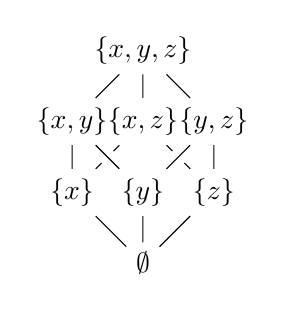
\begin{tikzpicture}[scale=0.45]
     
  \node (max) at (0,4) {$\{x,y,z\}$};
 \node (a) at (-2,2) {$\{x,y\}$};
 \node (b) at (0,2) {$\{x,z\}$};
 \node (c) at (2,2) {$\{y,z\}$};
 \node (d) at (-2,0) {$\{x\}$};
 \node (e) at (0,0) {$\{y\}$};
 \node (f) at (2,0) {$\{z\}$};
 \node (min) at (0,-2) {$\emptyset$};
 \draw (min) -- (d) -- (a) -- (max) -- (b) -- (f)
 (e) -- (min) -- (f) -- (c) -- (max)
 (d) -- (b);
 \draw[preaction={draw=white, -,line width=6pt}] (a) -- (e) -- (c);
          
  \end{tikzpicture}
	\caption{Hasse diagram}
	\end{figure}
\end{exampleblock}
\end{frame}
\begin{frame}{Lattice Theory}
\begin{definition}[least upper bound or join]
	A subset $S \subseteq P$ has a least upper bound (denoted $\sqcup S$ ) for     $(P,\preceq)$ if and only if:
	\begin{itemize} 
	\item  $\sqcup S \in P$ (the lub is an element of P)
	\item $ \forall x \in S~.~ x \preceq \sqcup S$ (the lub is an upper bound)
	\item $ \forall x \in S ~.~x \preceq u \Rightarrow \sqcup S \preceq u$ (\textbf{"minimum"} of the upper bounds)
\end{itemize}
\end{definition}
\begin{exampleblock}{Example:$(\mathcal{P}_S\{x,y,z\}, \subseteq)$}
	\begin{columns}
		\column{0.4\linewidth}
 	
   \tiny
  \usetikzlibrary{trees,shapes,decorations}
  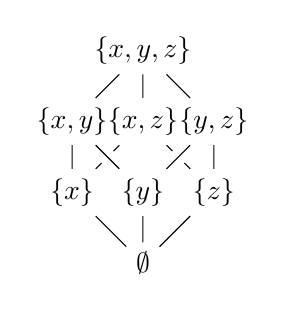
\begin{tikzpicture}[scale=0.45]
     
  \node (max) at (0,4) {$\{x,y,z\}$};
 \node (a) at (-2,2) {$\{x,y\}$};
 \node (b) at (0,2) {$\{x,z\}$};
 \node (c) at (2,2) {$\{y,z\}$};
 \node (d) at (-2,0) {$\{x\}$};
 \node (e) at (0,0) {$\{y\}$};
 \node (f) at (2,0) {$\{z\}$};
 \node (min) at (0,-2) {$\emptyset$};
 \draw (min) -- (d) -- (a) -- (max) -- (b) -- (f)
 (e) -- (min) -- (f) -- (c) -- (max)
 (d) -- (b);
 \draw[preaction={draw=white, -,line width=6pt}] (a) -- (e) -- (c);
          
  \end{tikzpicture}
 \column{0.6\linewidth}
 \footnotesize
 \begin{itemize}
 	\item  $\sqcup\{\{x\},\{z\}\}= \{y,z\}$
 	\item  $\sqcup\{\{x\},\{x,z\}\}=\{x,z\}$
 	\item  $\sqcup\{\emptyset,\{x,y,z\}\}=$??
 	\item  $\sqcup \{\{x\},\{y,z\}\}=$ ??
 \end{itemize}
	\end{columns}
\end{exampleblock}
\end{frame}


\begin{frame}{Lattice Theory}
\begin{definition}[greatest lower bound or meet]
	A subset $S \subseteq P$ has an greatest lower bound (denoted $\sqcap S$ ) for     $(P,\preceq)$ if and only if:
	\begin{itemize} 
		\item  $\sqcap S \in P$ (the glb is an element of P)
		\item $ \forall x \in S~.~   \sqcap S \preceq x$ (the lub is a lower bound)
		\item $ \forall x \in S ~.~l \preceq x \Rightarrow l \preceq \sqcap S  $ (\textbf{"maximum"} of the lower bounds)
	\end{itemize}
\end{definition}
\begin{exampleblock}{Example:$(\mathcal{P}_S\{x,y,z\}, \subseteq)$}
	\begin{columns}
		\column{0.4\linewidth}
		  \tiny
  \usetikzlibrary{trees,shapes,decorations}
  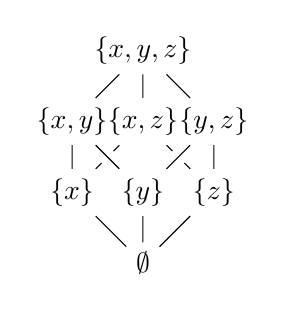
\begin{tikzpicture}[scale=0.45]
     
  \node (max) at (0,4) {$\{x,y,z\}$};
 \node (a) at (-2,2) {$\{x,y\}$};
 \node (b) at (0,2) {$\{x,z\}$};
 \node (c) at (2,2) {$\{y,z\}$};
 \node (d) at (-2,0) {$\{x\}$};
 \node (e) at (0,0) {$\{y\}$};
 \node (f) at (2,0) {$\{z\}$};
 \node (min) at (0,-2) {$\emptyset$};
 \draw (min) -- (d) -- (a) -- (max) -- (b) -- (f)
 (e) -- (min) -- (f) -- (c) -- (max)
 (d) -- (b);
 \draw[preaction={draw=white, -,line width=6pt}] (a) -- (e) -- (c);
          
  \end{tikzpicture}
		\column{0.6\linewidth}
		\footnotesize
		\begin{itemize}
			\item  $\sqcap\{\{x\},\{z\}\}= \emptyset$
			\item  $\sqcap\{\{x\},\{x,z\}\}=\{x\}$
			\item  $\sqcap\{\emptyset,\{x,y,z\}\}=$??
			\item  $\sqcap \{\{x\},\{y,z\}\}=$ ??
		\end{itemize}
	\end{columns}
\end{exampleblock}
\end{frame}

\begin{frame}{Lattice Theory}
\begin{definition}[Complete Lattice]
	A partial order $(P,\preceq)$ is a complete lattice if and only if for every  $S    \subseteq P$ the $\sqcup S$ and $\sqcap S$ are  defined.
\end{definition}

\begin{definition}[Least element and greatest element]
	A complete lattice  $(P,\preceq)$ has a maximal element $\top = \sqcup P$ and a minimal element  $\bot = \sqcap P$
\end{definition}

\begin{exampleblock}{Example:$(\mathcal{P}_S\{x,y,z\}, \subseteq)$ is a complete lattice}
	\begin{columns}
		\column{0.4\linewidth}
		\input{content/images/static-analysis/poset1}
		\column{0.6\linewidth}
		\footnotesize
		\begin{itemize}
			\item  $\top = \sqcup \mathcal{P}_S\{x,y,z\}=\{x,y,z\}$
		     \item  $\bot = \sqcap \mathcal{P}_S\{x,y,z\}=\emptyset$
		\end{itemize}
	\end{columns}
\end{exampleblock}
\end{frame}

\begin{frame}{Lattice Theory}{Function monotonicity and fixed point}
\begin{definition}[Increasing function]
	A function $F: P \rightarrow P$ is said to be increasing over $(P,\preceq) $ (written  $F: P \xrightarrow{\scriptscriptstyle \nearrow} P$) if only if:
	\begin{itemize}
		\item $\forall x, y \in P.~x \preceq y \Rightarrow F(x) \preceq F(y)$
	\end{itemize}
\end{definition}

\begin{definition}[Function fixpoint]
	A function $F: P\rightarrow P$ has a fixpoint $\phi$ if and only if: 
	\begin{itemize}
		\item $\phi \in P$.
		\item $F(\phi)=\phi$
	\end{itemize}
\end{definition}



\begin{exampleblock}{Example: fixed point}
let 	$f :\mathbb{Z}  \rightarrow \mathbb{Z} , f(x)= x^2 - 3x +4 $\\
$f(2)=2$ and $f(f(f...(2)))=2$\\

$g :\mathbb{Z}  \rightarrow \mathbb{Z} , g(x)= x^2$ ??
\end{exampleblock}
\end{frame}

\begin{frame}{Lattice Theory}{Tarski theorem}
\begin{theorem}[Fixpoint theorem:Tarski Knaster]
For a complete lattice $(P,\preceq)$ and a function  $f: P  \xrightarrow{\scriptscriptstyle \nearrow} P$ we have:
\begin{enumerate}
\item f is guaranteed to have a fixpoint $\phi$.
\item f may have several fixpoints, from which a least fixpoint $lfp_f$ and a $gfp_f$.
\item  $lfp_f= \sqcup \{f^k (\bot). k \in \mathbb{N}\}$ \\( where $  \scriptstyle f^k(x)=f(f^{k-1}(x))$.)  
\end{enumerate}
\end{theorem}
\centering \includegraphics[scale=0.25]{content/images/static-analysis/lfp.png}
\end{frame}


\begin{frame}{Data Flow Analysis meets Tarski Theorem}
\begin{itemize}
	\item If the domain of values $\mathbb{V}$ can for a  lattice($\mathbb(V),\preceq $). 
	\item If  the transfer function $Tf: \mathbb{V}  \xrightarrow{\scriptscriptstyle \nearrow} \mathbb{V} $.
	\item Then we are guaranteed to reach a least fixpoint, which is the most precise solution in $\mathbb{V}$.
	\item Then ($ \mathbb{V}, Tf, \sqcup_ \preceq)$ a \textcolor{blue}{monotonic framework}.
	\item There is no generic monotonic framework for constant propagation.
	\item The difficulty is to design a suitable $\mathbb{V}, Tf$  program (represented by the set of program labels $\mathbb{L}$ ). 
	\item Precision vs. convergence.
\end{itemize}
\end{frame}


\begin{frame}{Monotonic Framework Example}

\begin{columns}
	\column{0.4\linewidth}
	\begin{figure}
		\centering  \tiny
  \usetikzlibrary{trees,shapes,decorations}
  \begin{tikzpicture}[%
    ->,
    >=stealth,
    node distance=0.3cm,
    noname/.style={%
      rectangle,
      minimum width=5em,
      minimum height=2em,
      draw
    }
  ]
    \node[noname] (1)                                             {[ x = 1; ] $l_1$};
    \node[noname] (2) [below=of 1]                                {[ while(??) ] $l_2$};
    \node[noname] (3) [below = 1cm of 2]                                {[ x = x+1; ] $l_3$};
    \node[noname] (4) [below right= 1cm of 2]                                {[ ;; ] $l_4$};
    
   
    

      \path 
   (1) edge                          node {} (2)
   (2) edge     [bend right=45pt]                     node  [yshift=5pt,right]{yes} (3)
   (2) edge                                         node  [yshift=5pt,right]{no} (4)
   (3) edge [bend right=45pt]                        node {} (2);
 
          
  \end{tikzpicture}\\
		\vspace{1cm}
		%\lstinputlisting[language=C, basicstyle =\scriptsize]{content/images/static-analysis/whileloop.c}
		\centering  \tiny
  \usetikzlibrary{trees,shapes,decorations}
  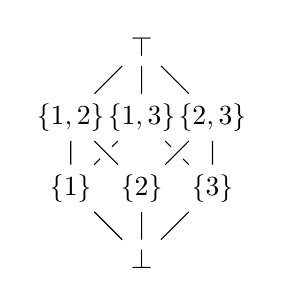
\begin{tikzpicture}[scale=0.45]
     
  \node (mam) at (0,4) {$\top$};
 \node (a) at (-2,2) {$\{1,2\}$};
 \node (b) at (0,2) {$\{1,3\}$};
 \node (c) at (2,2) {$\{2,3\}$};
 \node (d) at (-2,0) {$\{1\}$};
 \node (e) at (0,0) {$\{2\}$};
 \node (f) at (2,0) {$\{3\}$};
 \node (min) at (0,-2) {$\bot$};
 \draw (min) -- (d) -- (a) -- (mam) -- (b) -- (f)
 (e) -- (min) -- (f) -- (c) -- (mam)
 (d) -- (b);
 \draw[preaction={draw=white, -,line width=6pt}] (a) -- (e) -- (c);
          
  \end{tikzpicture}
	\end{figure}
	\column{0.6\linewidth}

	What is the result???
	
\end{columns}
\end{frame}

\begin{frame}{Monotonic Framework Example}

\begin{columns}
	\column{0.4\linewidth}
	\begin{figure}
	\centering  \tiny
  \usetikzlibrary{trees,shapes,decorations}
  \begin{tikzpicture}[%
    ->,
    >=stealth,
    node distance=0.3cm,
    noname/.style={%
      rectangle,
      minimum width=5em,
      minimum height=2em,
      draw
    }
  ]
    \node[noname] (1)                                             {[ x = 1; ] $l_1$};
    \node[noname] (2) [below=of 1]                                {[ while(??) ] $l_2$};
    \node[noname] (3) [below = 1cm of 2]                                {[ x = x+1; ] $l_3$};
    \node[noname] (4) [below right= 1cm of 2]                                {[ ;; ] $l_4$};
    
   
    

      \path 
   (1) edge                          node {} (2)
   (2) edge     [bend right=45pt]                     node  [yshift=5pt,right]{yes} (3)
   (2) edge                                         node  [yshift=5pt,right]{no} (4)
   (3) edge [bend right=45pt]                        node {} (2);
 
          
  \end{tikzpicture}\\
	\vspace{1cm}
	%\lstinputlisting[language=C, basicstyle =\scriptsize]{content/images/static-analysis/whileloop.c}
	\centering  \tiny
  \usetikzlibrary{trees,shapes,decorations}
  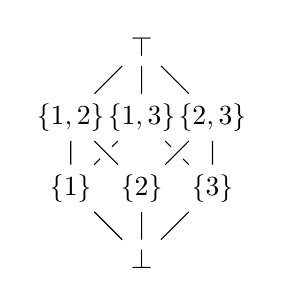
\begin{tikzpicture}[scale=0.45]
     
  \node (mam) at (0,4) {$\top$};
 \node (a) at (-2,2) {$\{1,2\}$};
 \node (b) at (0,2) {$\{1,3\}$};
 \node (c) at (2,2) {$\{2,3\}$};
 \node (d) at (-2,0) {$\{1\}$};
 \node (e) at (0,0) {$\{2\}$};
 \node (f) at (2,0) {$\{3\}$};
 \node (min) at (0,-2) {$\bot$};
 \draw (min) -- (d) -- (a) -- (mam) -- (b) -- (f)
 (e) -- (min) -- (f) -- (c) -- (mam)
 (d) -- (b);
 \draw[preaction={draw=white, -,line width=6pt}] (a) -- (e) -- (c);
          
  \end{tikzpicture}
    \end{figure}
	\column{0.6\linewidth}
	\begin{enumerate}\scriptsize
		\item $ \scriptstyle in_{l3}=in_{l2}=in_{l1}=\bot$ \scriptsize \textcolor{blue}{(initialization)}
		\item $ \scriptstyle  x_{l1}^1 =Tf_{l1}^1 (in_{l1})= \{1\}$
		\item $ \scriptstyle in_{l2}^1 = \sqcup(out_{l1},out_{l2})=\sqcup(\{1\}, \bot) =\{1\} $
		\item $ \scriptstyle x_{l3}^1= in_{l2}^1+ \{1\} = \{2\} $
		\item $ \scriptstyle in_{l2}^2 = \sqcup(1, 2) = \{1,2\}$
		\item $ \scriptstyle x_{l3}^2= in_{l2}^2+1 = \{1,2\} + \{1\} =\{2,3\}$
		\item $ \scriptstyle in_{l2}^2 = \sqcup(\{2,3\}, \{1\}) = \top \wedge x_{l2}^2=in_{l2}^2 $
		\item $\scriptstyle x_{l3}^3 =Tf_{l3}^3(\top)=\top $ \scriptsize \textcolor{blue}{(fixpoint reached) }
	\end{enumerate}
     \scriptsize
     $\top$ means the set of all possible values or the result is failing(all the possible values).\\
     the result will be the same of all the possible set lattices of $ ( S \subset \mathbb{Z}, \subseteq)$ if the iterations terminates. 
     
\end{columns}
\end{frame}

\begin{frame}{Data Flow: Wrap-Up}
\begin{itemize}
\item Monotonic frameworks ensures data flow analyses termination or \textcolor{blue}{Inductive program verification}.
\item The analysis is ensured by induction over the collecting semantics of the programming language.
\item The induction is defined because of the fixpoint theorem.
\item The results are not always precise and hard to tune.
\item Another way to analyse : approximating the programs properties.
\item \textcolor{blue}{Abstract program analysis}: analysis on Abstract domains to get meaningful approximations than the result concrete domains.
\end{itemize}
\end{frame}

\section{Analysis by Abstract Interpretation}
\begin{frame}{By Patrick and Radia Cousot}
\centering
\includegraphics[scale=0.60]{content/images/static-analysis/Abstractcousot.png}
\end{frame}


\begin{frame}{What is on the program}
\begin{itemize}
	\item Informal introduction.
	\item Galois connection for abstract interpretation.
	\item Interval abstract domain.
	\item widening, narrowing.
\end{itemize}
\end{frame}



\begin{frame}{Informal Introduction:}
\begin{itemize}
	\item Abstractions are an intuitive notion.
	\item Abstraction is on abstract domains.
	\item $[-\infty, +\infty] $ is an abstraction of $\mathbb{Z}$ in the interval domain. 
	\item Negative is an abstraction of $-2$ in the sign domain.
	\item Abstraction is an approximation.
\end{itemize}
\end{frame}



\begin{frame}{Undecidability}
\textit{"All interesting properties of the behavior of programs written in common programming languages are mathematically \textbf{undecidable}."} From Rice's Theorem [1953]

\textbf{Undecidable:}
\begin{itemize}
	\item \textbf{Among the solutions}: 
	\begin{enumerate}
		\item Identify a subclass of programs for which the verification problem is decidable.
		\item \textcolor{blue}{Approximate (Partial correctness, sound approximation)}. 
		\item Use dynamic methods to complement.		
	\end{enumerate}
\item \textcolor{blue}{Soundness}:The software contains a bug $\Rightarrow$  Run of the algorithm will detect it. \textbf{(No False negative)}.
\item What is a sound approximation?
\end{itemize} 
\end{frame}


\begin{frame}{Informal Introduction: Over/under Approximations}
\centering\documentclass[tikz,border=2mm]{standalone}
\begin{document}
\begin{tikzpicture}
\draw[help lines, color=gray!30, dashed] (-4.9,-4.9) grid (4.9,4.9);
\draw[->,ultra thick] (-5,0)--(5,0) node[right]{$x$};
\draw[->,ultra thick] (0,-5)--(0,5) node[above]{$y$};

\end{tikzpicture}
\end{document}
\begin{itemize}
	\item \textcolor{blue}{Values computed by the program}
	\item \textbf{Not always analysable: $\top$} is the result of the data flow analysis.
	\item We need to approximate, but why?

\end{itemize}
\end{frame}

\begin{frame}{Informal Introduction: Approximations}
\centering
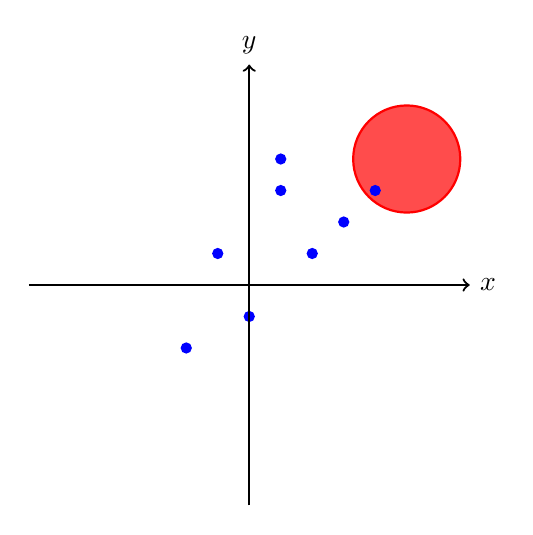
\begin{tikzpicture}[thick, scale=0.4,dot/.style={fill=blue,circle,minimum size=1pt}]




%\filldraw [fill=orange!10,draw=orange,thick] (0,1) circle (5.4);

%\filldraw [fill=yellow!70,draw=yellow,thick] (0,1) circle (3);
%\filldraw [fill=green!10,draw=green,thick]
%(-2.3, -3.3) rectangle (4.5, 4.5);
\filldraw [fill=red!70,draw=red,thick] (5,4) circle (1.70);



\filldraw [blue] (-1,1) circle (4pt)
(1,3) circle  (4pt)
(3,2) circle (4pt)
(4,3) circle (4pt)
(1,3) circle (4pt)
(1,4) circle (4pt)
(0,-1) circle (4pt)
%(2,-3) circle (4pt)
(2,1) circle (4pt)
(-2,-2) circle (4pt);
\draw[->, thick] (-7,0)--(7,0) node[right]{$x$};
\draw[->, thick] (0,-7)--(0,7) node[above]{$y$};


\end{tikzpicture}

\begin{itemize}
	\item \textcolor{blue}{Values computed by the program}
	\item \textbf{Not always analysable: when $\top$} is the analysis result.
	\item \textcolor{red}{ Bad states: causing bugs or violating a property.}
	\item We need to approximate.
\end{itemize}
\end{frame}

\begin{frame}{Informal Introduction: Over-/under-approximations}
\centering\input{content/images/static-analysis/under-approx}
\begin{itemize}
	\item \textcolor{blue}{Values computed by the program}.
	\item  \textcolor{orange}{Over-approximation}.
	\item  \textcolor{cyan}{Under-approximation}.
	\item \textbf{\textcolor{black}{ Which approximation is more suited for detecting "bad states"?}}
	
\end{itemize}
\end{frame}

\begin{frame}{Informal Introduction: Over/under-approximations}
\centering\input{content/images/static-analysis/over-er}
\begin{itemize}
	\item \textcolor{blue}{Values computed by the program}.
		\item \textcolor{red}{ Bad states: causing bugs or violating a property.}
	\item \textcolor{orange}{Over-approximation}, result is  \textbf{Yes}: $\surd$
	\item \textcolor{cyan}{Under-approximation},  result is  \textbf{No}:\textbf{ False negative}.   
	\item Over-approximation is sound.
\end{itemize}
\end{frame}
\begin{frame}{Informal Introduction: Over/under Approximations}
\centering\input{content/images/static-analysis/over-er1}
\begin{itemize}
	\item \textcolor{blue}{Values computed by the program}.
	\item \textcolor{red}{ Bad states: causing bugs or violating a property.}
	\item \textcolor{orange}{Over-approximation}, result is  \textbf{Yes}: False positive.  
	\item Over-approximation is not complete.
\end{itemize}
\end{frame}


\begin{frame}{What is Abstract interpretation?}
\begin{itemize}
	\item A \textcolor{blue}{mathematical theory} formalizing the abstraction of program semantic properties.
	\item Used to reason on and to calculate \textcolor{blue}{abstract program properties}.
	\item Applications: program semantics, verification, dynamic and \textcolor{blue}{static analysis of software}.
	\end{itemize}
\end{frame}

\begin{frame}{Informal Introduction:}
\begin{itemize}
	\item let \textcolor{blue}{$(\mathcal{C}, \preceq_c)$} a domain  of concrete values.
	\item let \textcolor{blue}{$(\mathcal{A}, \preceq_a)$} a domain of abstract values.
	\item Abstraction function \textcolor{blue}{$\alpha: \mathcal{C} \rightarrow \mathcal{A}$}.
	\item Concretization function \textcolor{blue}{$\gamma : \mathcal{A} \rightarrow \mathcal{B}$}.
	\item Suppose we want to verify a property \textcolor{blue}{$Prop \subset \mathcal{C}$}.
	\item Analyse the Program in the abstract domain \textcolor{blue}{$(\mathcal{A}, \preceq_a)$}, we need an abstract functions to obtain $Result^\sharp$.
	 \begin{enumerate}
	\item Concretize  \textcolor{blue}{$Result= \gamma(Result^\sharp)$} and check for \textcolor{blue}{$Prop$}.
	\item Abstract the property \textcolor{blue}{$Prop^\sharp = \alpha(Prop)$} and check with \textcolor{blue}{$Result^\sharp$}.
	\end{enumerate}
\end{itemize}
\end{frame}

\begin{frame}{First abstract domain: Sign abstract domain}
\begin{itemize}
	\item By Brahmagupta (born c.  598-670)) was an Indian mathematician and
	astronomer.
	\item Invented the rule of signs (including to compute with zero).
	\item Let's understand this reasoning in term of Abstract interpretation.
\end{itemize}
\end{frame}


\begin{frame}{First abstract domain: Sign abstract domain}
\centering \includegraphics[scale=0.50]{content/images/static-analysis/sign.png}
\begin{itemize}
	\item $(\mathbb{P}^\pm, \subseteq_\pm)$ is the sign abstract domain.
	\item $(\mathcal{P_S}(\mathbb{Z}),\subseteq)$ be the concrete domain.
	\item The sign abstract domain is a complete lattice.
\end{itemize}
\end{frame}

\begin{frame}{First abstract domain: Sign abstract domain}
\begin{itemize}
	\item $(\mathbb{P}^\pm, \subseteq_\pm)$ is the sign abstract domain.
	\item $(\mathcal{P_S}(\mathbb{Z}),\subseteq)$ be the concrete domain.
	\item The abstraction function is defined as $\alpha^{\pm}: \mathbb{Z} \rightarrow \mathbb{P}^{\pm}+$:\newline
$\forall e \subseteq \mathbb{Z}: \alpha_\pm(e)     \left\{ \begin{array}{rcl}
\bot_{\pm} & \mbox{if}& e= \emptyset \\
=0  & \mbox{else if} & e \subseteq \{0\} \\
>0 & \mbox{else if} & e \subseteq \{x \in \mathbb{Z} |~ x >0\}\\
<0 & \mbox{else if} & e\subseteq \{x \in \mathbb{Z} |~ x <0\}\\
\leq 0 & \mbox{else if} & e\subseteq \{x \in \mathbb{Z} | ~x  \leq 0\}\\
\geq 0 & \mbox{else if} & e\subseteq \{x \in \mathbb{Z} |~ x  \geq 0\}\\
\neq 0 & \mbox{else if} & e\subseteq \{x \in \mathbb{Z} |~ x  \neq 0\}\\
\top_\pm & \mbox{else} & 
\end{array}\right.$
\end{itemize}
\begin{exampleblock}{Examples:}
	$    \begin{array}{l l}
\alpha^{\pm}(\{1,3,7\})=~>0 & \alpha^{\pm}(\{0,1,3,7\})=~\geq 0 \\
\alpha^{\pm}(\{-1,7\})=~ ?? & \alpha^{\pm}(\{-16,0,1,7\})=~ ?? \\
\end{array}$
\end{exampleblock}
\end{frame}

\begin{frame}{First abstract domain: Sign abstract domain}
\begin{itemize}
	\item $(\mathbb{P}^\pm, \subseteq_\pm)$ is the sign abstract domain.
	\item $(\mathcal{P_S}(\mathbb{Z}),\subseteq)$ be the concrete domain.
	\item The sign concretization function is defined as $\gamma_\pm:  \mathbb{P}^{\pm} \rightarrow \mathbb{Z}$:
	
	$    \begin{array}{l l}
\gamma^{\pm}(\bot^{\pm}) = \emptyset &  \gamma^{\pm}(=0)=\{0\} \\ 
\gamma_\pm(>0)=\{x \in \mathbb{Z} |~ x >0\}	 & \gamma_\pm(<0)=\{x \in \mathbb{Z} |~ x <0\} \\
\gamma_\pm(\leq0)=\{x \in \mathbb{Z} |~ x \leq 0\}	 & \gamma_\pm(\geq 0)=\{x \in \mathbb{Z} |~ x \geq 0\} \\
\gamma_\pm(\neq 0)=\{x \in \mathbb{Z} |~ x \neq 0\}	 & \gamma_\pm(\top^{\pm})=\mathbb{Z} \\
\end{array}.$
\end{itemize}
\end{frame}

\begin{frame}{Abstract interpretation: Galois connections}
\begin{definition}[Galois connection]
 $(\mathcal{C}, \preceq_c) \galois{\alpha}{\gamma} (\mathcal{A}, \preceq_a)$ is a Galois connection iff:
 \begin{enumerate}
 \item $\gamma$ is increasing;
 \item $\alpha$ is increasing;
 \item $\forall x \in \mathcal{C}~. ~x \preceq_c \gamma \comp \alpha(x)$ ($\gamma \comp \alpha$ is extensive)
 \item $\forall y \in \mathcal{A}~.~ \alpha \comp \gamma(y) \preceq_a y$ ($\alpha \comp \gamma$ is reductive)
 \end{enumerate}
\end{definition}

\begin{exampleblock}{Examples:$(\mathbb{Z}, \subseteq) \galois{\alpha_\pm}{\gamma_\pm} (\mathbb{P}_{\pm}, \subseteq_{\pm})$}
	
	$\begin{array}{l l l}
	\scriptstyle \gamma_\pm\comp \alpha_\pm (\{1,2,3\})= \{x \in \mathbb{Z} |~ x >0\} & \text{and} &\scriptstyle\alpha_\pm\comp \gamma_\pm(>0) =~>0  \\
	\scriptstyle \{1,2,3\} \subseteq  \{x \in \mathbb{Z} |~ x >0\} & \text{and}  & \scriptstyle>0 ~\subseteq_\pm~ >0
	\end{array}$
\end{exampleblock}
\end{frame}
	
\begin{frame}{Best abstract transfer function}
\begin{definition}[Best abstract transformer]
$(\mathcal{C}, \preceq_c) \galois{\alpha}{\gamma} (\mathcal{A}, \preceq_a)$ and $F:\mathcal{C} \rightarrow \mathcal{C}$, the best abstract function $F^{\scriptsize \sharp}_b: \mathcal{A}\rightarrow\mathcal{A}$ is defined as:
\begin{itemize}
	\item $F^{\scriptsize \sharp}_b(y) \triangleq \alpha \comp F \comp \gamma (y)$
\end{itemize}
\end{definition}

 \begin{alertblock}{The best abstract transfer function does not always exist:}
 	\begin{itemize}
	\item In practice, $\alpha \comp TF \comp \gamma$ is not computable or too complex.
	\item Also, sometimes either  $\alpha$/$\gamma$ is not defined.	
	\item The solution is to define  $ TF^{\scriptsize \sharp}_b\preceq_\sharp TF^{\scriptsize \sharp} $
    \end{itemize}
\end{alertblock}
\end{frame}


\begin{frame}{Collecting semantics for the sign abstract domain with 1 variable x}
\begin{itemize}
	\item \scriptsize The set of sign transfer functions is defined as: \\$in_{li}=\sqcup(x_{pre_{li}})$ and $ x_{l_i}= TF^{\scriptscriptstyle \pm}_{l_i}(in_{l_i})$\\
	$  TF^{\scriptscriptstyle \pm}_{l_i}(in_{l_i}) =     \left\{ \begin{array}{rcl}
\textstyle	in_{l_i} &  \mbox{\scriptsize if}& \textstyle l_i~\text{\scriptsize is}~while(B)~\mid~ if(B) ~\mid~;;   \\
\textstyle	\|a\|_{li}^{\scriptscriptstyle \pm}  & \mbox{\scriptsize if} & \textstyle l_i~\mbox{\scriptsize is}~x~=~a; \\
\scriptstyle	\|a\|_{li}^{\scriptscriptstyle \pm}~op_\pm~ \|b\|_{li}^{\scriptscriptstyle \pm}  & \mbox{\scriptsize if} &  \textstyle l_i~\mbox{\scriptsize is}~x~=~a~op_a~b; \\
	\dots & \mbox{if} & \dots
	\end{array}\right.$
	
	\item \scriptsize The abstract evaluation function:\\  $ \|a\|_{li}^{\scriptscriptstyle \pm} =     \left\{ \begin{array}{rcl}
	in_{l_i} & \mbox{ if}&  \text{x is a variable}   \\
	\gamma_{\pm}(a)  & \mbox{ if} &  \text{x is a a constant value} 
\end{array}\right.$
\item The set of abstract arithmetic operator: $op_\pm=\{+_{\scriptscriptstyle \pm}, -_{\scriptscriptstyle \pm}, \times_{\scriptscriptstyle \pm}\}$
\end{itemize}
\centering \includegraphics[scale=0.40]{content/images/static-analysis/minus-sign.png}
\end{frame}

\begin{frame}{While example in the sign domain:}
\begin{exampleblock}{while loop:1}
	\centering   \tiny
  \usetikzlibrary{trees,shapes,decorations}
  \begin{tikzpicture}[%
    ->,
    >=stealth,
    node distance=0.3cm,
    noname/.style={%
      rectangle,
      minimum width=5em,
      minimum height=2em,
      draw
    }
  ]
    \node[noname] (1)                                             {[ x = 1; ] $l_1$};
    \node[noname] (2) [below=of 1]                                {[ while(??) ] $l_2$};
    \node[noname] (3) [below = 1cm of 2]                                {[ x = x+1; ] $l_3$};
    \node[noname] (4) [below right= 1cm of 2]                                {[ ;; ] $l_4$};
    
   
    

      \path 
   (1) edge                          node {} (2)
   (2) edge     [bend right=45pt]                     node  [yshift=5pt,right]{yes} (3)
   (2) edge                                         node  [yshift=5pt,right]{no} (4)
   (3) edge [bend right=45pt]                        node {} (2);
 
          
  \end{tikzpicture}
	\centering \includegraphics[scale=0.60]{content/images/static-analysis/sign1.png}
	
	\begin{itemize}
		\item Initialization: 
			\\ $\scriptsize in_{l_1}=in_{l_2}=in_{l_3}=in_{l_4}=~\bot^{\pm}$
			\\ $\scriptsize x_{l_1}^0 =~>0~;~~x_{l_2}^0 =~~>0~;~~x_{l_3}^0 =~~>0~;~~x_{l_4}^0 =~>0~~$
			
		\end{itemize}
\end{exampleblock}
\end{frame}

\begin{frame}{While example in the sign domain:}
\begin{exampleblock}{while loop:2}
	\centering   \tiny
  \usetikzlibrary{trees,shapes,decorations}
  \begin{tikzpicture}[%
    ->,
    >=stealth,
    node distance=0.3cm,
    noname/.style={%
      rectangle,
      minimum width=5em,
      minimum height=2em,
      draw
    }
  ]
    \node[noname] (1)                                             {[ x = 1; ] $l_1$};
    \node[noname] (2) [below=of 1]                                {[ while(??) ] $l_2$};
    \node[noname] (3) [below = 1cm of 2]                                {[ x = x+1; ] $l_3$};
    \node[noname] (4) [below right= 1cm of 2]                                {[ ;; ] $l_4$};
    
   
    

      \path 
   (1) edge                          node {} (2)
   (2) edge     [bend right=45pt]                     node  [yshift=5pt,right]{yes} (3)
   (2) edge                                         node  [yshift=5pt,right]{no} (4)
   (3) edge [bend right=45pt]                        node {} (2);
 
          
  \end{tikzpicture}
	\centering \includegraphics[scale=0.60]{content/images/static-analysis/sign1.png}
	
	\begin{itemize}
		\item Initialization: 
		\\ $\scriptsize in_{l_1}=in_{l_2}=in_{l_3}=in_{l_4}=\bot^{\pm}$
		\\ $\scriptsize x_{l_1}^0 =~>0~;~~x_{l_2}^0 =~>0~;~~x_{l_3}^0 =~>0~;~~x_{l_4}^0 =~>0~~~$
		
		\item First iteration: $x_{l_1}^1 = ~>0 = x_{l_1}^0 $ fixpoint for $l_1$ 
		\item Second iteration: $x_{l_2}^2 = ~>0  =  x_{l_2}^0 $ fixpoint for $l_2$ 
		\item Third iteration: $x_{l_3}^4 = ~>0 = x_{l_4}^0 $ fixpoint for $l_3$ 
		\item Fourth iteration $x_{l_4}^5 =~ >0 = x_{l_4}^0 $ fixpoint for $l_4$ and $worklist=\emptyset$
		\item The result of the analysis is: $>0$
	\end{itemize}
\end{exampleblock}
\end{frame}

\begin{frame}{While example1:}
\begin{exampleblock}{while loop:1}
	\centering   \tiny
  \usetikzlibrary{trees,shapes,decorations}
  \begin{tikzpicture}[%
    ->,
    >=stealth,
    node distance=0.3cm,
    noname/.style={%
      rectangle,
      minimum width=5em,
      minimum height=2em,
      draw
    }
  ]
    \node[noname] (1)                                             {[ x = 1; ] $l_1$};
    \node[noname] (2) [below=of 1]                                {[ while(??) ] $l_2$};
    \node[noname] (3) [below = 1cm of 2]                                {[ x = x+1; ] $l_3$};
    \node[noname] (4) [below right= 1cm of 2]                                {[ ;; ] $l_4$};
    
   
    

      \path 
   (1) edge                          node {} (2)
   (2) edge     [bend right=45pt]                     node  [yshift=5pt,right]{yes} (3)
   (2) edge                                         node  [yshift=5pt,right]{no} (4)
   (3) edge [bend right=45pt]                        node {} (2);
 
          
  \end{tikzpicture}
	\centering \includegraphics[scale=0.60]{content/images/static-analysis/sign1.png}
			\begin{enumerate}
				\item The abstract solution is: $Result^{\pm}~=~>0$ for  $(\mathbb{P}^\pm, \subseteq_\pm)$ with $TF^{\scriptscriptstyle \pm}$
				\item The concretization is : $\gamma_{\pm}(>0)= \{z \in \mathbb{Z} ~|~ z>0 \}$
				\item The result was $\top$ for $(\mathbb{Z}, \subseteq)$ with $TF$
			    \item $\gamma_{\pm}(Result^{\pm})=\{z \in \mathbb{Z} ~|~ z>0 \} \subseteq \top$  in the concrete domain.
			    \item The real values of the program are: $\{z \in \mathbb{Z} ~|~ z \geq 1 \} \equiv_{\mathbb{Z}} {\displaystyle \gamma}_{\pm}(Result^{\pm})$
			    \item Can we do better with another abstract domain for this program?
			    \item Are the results of $TF^\pm$ always more precise than $TF$??
				\end{enumerate}
	
\end{exampleblock}
\end{frame}

\begin{frame}{Precision ???}
\begin{exampleblock}{if example in the sign framework }
	Analyse the following program using $TF$ and $TF^{\pm}$, and compare their results.
\lstinputlisting[language=C, basicstyle =\tiny]{content/images/static-analysis/precision.c}
	\end{exampleblock}
\end{frame}


\begin{frame}{Interval domain:$(\mathcal{I}, \sqsubseteq )$}\
\centering \includegraphics[scale=0.45]{content/images/static-analysis/interval.png}
\end{frame}

\begin{frame}{Interval domain:$(\mathcal{I}, \sqsubseteq )$}
\begin{itemize}
\item $(\mathcal{I}, \sqsubseteq )$ is a complete lattice.
\item $(\mathcal{I}, \sqsubseteq )$ with enumerable element but is countably infinite.
\item \textcolor{orange}{Problem 1}: can't infer the $\sqcup_{\scriptscriptstyle \sqsubseteq}$ from the Hasse diagram.
\item \textcolor{orange}{Problem 2}: ??
\end{itemize}
\end{frame}


\begin{frame}{Interval domain:$(\mathcal{I}, \sqsubseteq )$}
\begin{itemize}
	\item $(\mathcal{I}, \sqsubseteq )$ is a complete lattice.
	\item $(\mathcal{I}, \sqsubseteq )$ with enumerable elements but is \textcolor{orange}{countably infinite}.
	\item \textcolor{orange}{Problem 1}: can't infer the $\sqcup_{\scriptscriptstyle \sqsubseteq}$ from the Hasse diagram.
	\begin{itemize}
		\item Define $\sqcup_{\scriptscriptstyle \sqsubseteq}$
   \end{itemize}
	\item \textcolor{orange}{Problem 2}: ??
\end{itemize}
\end{frame}

\begin{frame}{Interval domain: join operator  $\sqcup_{\scriptscriptstyle \sqsubseteq}$}
\begin{itemize}
	\item Can be defined using  $\sqcup_\subseteq$ from $(\mathcal{P}_S(\mathbb{Z}), \subseteq)$.
	\item Can also be defined using $min$ and $max$ functions.
	\item $\sqcup_{\scriptscriptstyle \sqsubseteq}([a,b],[c,d])=[min(a,c),max(c,d)]$
	\item Set of axioms for $-\infty, \infty$:\\
	
	$  \forall x \in \mathbb{Z}     \left\{ \begin{array}{lcc}
	x  &  < & \infty  \\
	x  &  > & -\infty   \\
	-\infty &  < & \infty \\
\end{array}\right.$
\end{itemize}
\end{frame}

\begin{frame}{Interval domain: $\gamma_{\scriptscriptstyle\mathcal{I}}: \mathcal{I} \rightarrow \mathcal{P}_S(\mathbb{Z})$}
\begin{itemize}
	\item $\alpha_{\scriptscriptstyle\mathcal{I}}(x)=
	 \left\{ \begin{array}{lcc}
	\top^I~=~[-\infty,\infty]  &  \text{if} & x=\top  \\
	\bot^I~=~\emptyset  &  \text{if} & x=\bot \\
     I_x~=~[inf(x), sup(x)]   &  else &   \\
	\end{array}\right.$  
		\item $\gamma_{\scriptscriptstyle\mathcal{I}}(y)=
	\left\{ \begin{array}{lcl}
	\top &  \text{if} & y=\top^I  \\
	\bot~=~\emptyset  &  \text{if} & y=\bot^I \\
	\{x \in \mathbb{Z} ~|~ x \leq b \}&  \text{if} & y = [-\infty,b]  \\
	\{x \in \mathbb{Z} ~|~ a \leq x  \}&  \text{if} & y = [a,\infty]  \\
	\{x \in \mathbb{Z} ~|~ a \leq x \leq b\} &  \text{if} & y = [a,b]  \\
	\end{array}\right.$
\end{itemize}
\begin{exampleblock}{Examples:}
	
	$\begin{array}{l}
	 \gamma_{\scriptscriptstyle\mathcal{I}} \comp \alpha_{\scriptscriptstyle\mathcal{I}} (\{1,2,3\})= \gamma_{\scriptscriptstyle\mathcal{I}}([1,3])= {\scriptstyle \{x \in \mathbb{Z}~|~ 1 \leq x \leq 3\}} =\{1,2,3\}  \\
	 \{1,2,3\} =  \gamma_{\scriptscriptstyle\mathcal{I}} \comp \alpha_{\scriptscriptstyle\mathcal{I}} (\{1,2,3\})\\
 \gamma_{\scriptscriptstyle\mathcal{I}} \comp \alpha_{\scriptscriptstyle\mathcal{I}} (\{1,3\})= ??\\
	 \gamma_{\scriptscriptstyle\mathcal{I}} \comp \alpha_{\scriptscriptstyle\mathcal{I}} (\{x \in \mathbb{Z}~.~x\leq 1\})= ??
	\end{array}$\\
	
\end{exampleblock}
\end{frame}

\begin{frame}{Collecting semantics for the $(\mathcal{I},\sqsubseteq)$  domain with 1 variable x}
\begin{itemize}
	\item \scriptsize The set of Interval transfer functions is defined as:\\$in_{li}=\sqcup(x_{pre_{li}})$ and $ x_{l_i}= TF^{\scriptscriptstyle \mathcal{I}}_{l_i}(in_{l_i}),$\\ 
	$  TF^{\scriptscriptstyle \mathcal{I}}_{l_i}(in_{l_i}) =     \left\{ \begin{array}{rcl}
	\textstyle	in_{l_i} &  \mbox{\scriptsize if}& \textstyle l_i~\text{\scriptsize is}~while(B)~\mid~ if(B) ~\mid~;;   \\
	\textstyle	\|a\|_{li}^{\scriptscriptstyle \mathcal{I}}  & \mbox{\scriptsize if} & \textstyle l_i~\mbox{\scriptsize is}~x~=~a; \\
	\scriptstyle	\|a\|_{li}^{\scriptscriptstyle \mathcal{I}}~op_\mathcal{I}~ \|b\|_{li}^{\scriptscriptstyle \mathcal{I}}  & \mbox{\scriptsize if} &  \textstyle l_i~\mbox{\scriptsize is}~x~=~a~op_a~b; \\
	\dots & \mbox{if} & \dots
	\end{array}\right.$
	
	\item \scriptsize The abstract evaluation function:\\  $ \|a\|_{li}^ {\scriptscriptstyle \mathcal{I}} =     \left\{ \begin{array}{rcl}
	in_{l_i} & \mbox{ if}&  \text{x is a variable}   \\
	\gamma^{\scriptscriptstyle \mathcal{I}}(a)  & \mbox{ if} &  \text{x is a a constant value} 
	\end{array}\right.$
%	\item The set of abstract arithmetic operator:
%	 $op_{\scriptscriptstyle \mathcal{I}}\in \{+_{\scriptscriptstyle \mathcal{I}}, -_{\scriptscriptstyle \mathcal{I}}, \times_{\scriptscriptstyle \mathcal{I}}\}$
\end{itemize}

\end{frame}

\begin{frame}{Collecting semantics for the $(\mathcal{I},\sqsubseteq)$  domain with 1 variable x}
\begin{itemize}
	\item \scriptsize The set of Interval transfer functions is defined as: \\$in_{li}=\sqcup(x_{pre_{li}})$ and $ x_{l_i}= TF^{\scriptscriptstyle \mathcal{I}}_{l_i}(in_{l_i})$\\
	$  TF^{\scriptscriptstyle \mathcal{I}}_{l_i}(in_{l_i}) =     \left\{ \begin{array}{rcl}
	\textstyle	in_{l_i} &  \mbox{\scriptsize if}& \textstyle l_i~\text{\scriptsize is}~while(B)~\mid~ if(B) ~\mid~;;   \\
	\textstyle	\|a\|_{li}^{\scriptscriptstyle \mathcal{I}}  & \mbox{\scriptsize if} & \textstyle l_i~\mbox{\scriptsize is}~x~=~a; \\
	\scriptstyle	\|a\|_{li}^{\scriptscriptstyle \mathcal{I}}~op_\mathcal{I}~ \|b\|_{li}^{\scriptscriptstyle \mathcal{I}}  & \mbox{\scriptsize if} &  \textstyle l_i~\mbox{\scriptsize is}~x~=~a~op_a~b; \\
	\dots & \mbox{if} & \dots
	\end{array}\right.$
	
	\item \scriptsize The abstract evaluation function:\\  $ \|a\|_{li}^ {\scriptscriptstyle \mathcal{I}} =     \left\{ \begin{array}{rcl}
	in_{l_i} & \mbox{ if}&  \text{x is a variable}   \\
	\gamma^{\scriptscriptstyle \mathcal{I}}(a)  & \mbox{ if} &  \text{x is a a constant value} 
	\end{array}\right.$
		\item The set of abstract arithmetic operator:
		 $op_{\scriptscriptstyle \mathcal{I}}\in \{+_{\scriptscriptstyle \mathcal{I}}, -_{\scriptscriptstyle \mathcal{I}}, \times_{\scriptscriptstyle \mathcal{I}}\}$.\\
		 $op_{\scriptscriptstyle \mathcal{I}}: \mathcal{I} \times \mathcal{I} \rightarrow \mathcal{I}:$
		 
		 
		\begin{itemize}
		 	\item $\bot{\scriptscriptstyle \mathcal{I}} ~~op_{\scriptscriptstyle \mathcal{I}}~~ [a,b] = [a,b]~ op_{\scriptscriptstyle \mathcal{I}} ~\bot{\scriptscriptstyle \mathcal{I}} = ~\bot{\scriptscriptstyle \mathcal{I}}  $
		 	\item $[a,b] +_{\scriptscriptstyle \mathcal{I}}[c,d] = [a+c,b+d]$
		 	\item $[a,b] -_{\scriptscriptstyle \mathcal{I}}[c,d] = [a-d,b-c]$
		 	\item $ [a,b] \times_{\scriptscriptstyle \mathcal{I}}[c,d]=[min(B), max(B)] $\\ with $ B = \{(a \times c), (a \times d), (b\times c), (b \times d)\}$
		 \end{itemize}
		 
\end{itemize}
\end{frame}

\begin{frame}{While Example in the Interval Domain:}
\begin{exampleblock}{while loop:1}
	\centering   \tiny
  \usetikzlibrary{trees,shapes,decorations}
  \begin{tikzpicture}[%
    ->,
    >=stealth,
    node distance=0.3cm,
    noname/.style={%
      rectangle,
      minimum width=5em,
      minimum height=2em,
      draw
    }
  ]
    \node[noname] (1)                                             {[ x = 1; ] $l_1$};
    \node[noname] (2) [below=of 1]                                {[ while(??) ] $l_2$};
    \node[noname] (3) [below = 1cm of 2]                                {[ x = x+1; ] $l_3$};
    \node[noname] (4) [below right= 1cm of 2]                                {[ ;; ] $l_4$};
    
   
    

      \path 
   (1) edge                          node {} (2)
   (2) edge     [bend right=45pt]                     node  [yshift=5pt,right]{yes} (3)
   (2) edge                                         node  [yshift=5pt,right]{no} (4)
   (3) edge [bend right=45pt]                        node {} (2);
 
          
  \end{tikzpicture}
	\centering \includegraphics[scale=0.60]{content/images/static-analysis/sign1.png}
	
	\begin{itemize}
		\item Initialization: 
		\\ $\scriptsize in_{l_1}=in_{l_2}=in_{l_3}=in_{l_4}=\bot^{\mathcal{I}}$
		\\ $\scriptsize x_{l_1}^0 =?? ;~~x_{l_2}^0 =~??~;~~x_{l_3}^0 =~??~;~~x_{l_4}^0 =~??$
	\end{itemize}
\end{exampleblock}
\end{frame}

\begin{frame}{While Example in the Interval Domain:}
\begin{exampleblock}{while loop:2}
	\centering   \tiny
  \usetikzlibrary{trees,shapes,decorations}
  \begin{tikzpicture}[%
    ->,
    >=stealth,
    node distance=0.3cm,
    noname/.style={%
      rectangle,
      minimum width=5em,
      minimum height=2em,
      draw
    }
  ]
    \node[noname] (1)                                             {[ x = 1; ] $l_1$};
    \node[noname] (2) [below=of 1]                                {[ while(??) ] $l_2$};
    \node[noname] (3) [below = 1cm of 2]                                {[ x = x+1; ] $l_3$};
    \node[noname] (4) [below right= 1cm of 2]                                {[ ;; ] $l_4$};
    
   
    

      \path 
   (1) edge                          node {} (2)
   (2) edge     [bend right=45pt]                     node  [yshift=5pt,right]{yes} (3)
   (2) edge                                         node  [yshift=5pt,right]{no} (4)
   (3) edge [bend right=45pt]                        node {} (2);
 
          
  \end{tikzpicture}
	\centering \includegraphics[scale=0.60]{content/images/static-analysis/sign1.png}
	
	\begin{itemize}
		\item result??: 
		\\ $\scriptsize in_{l_1}~=~in_{l_2}=in_{l_3}=in_{l_4}=\bot^{\mathcal{I}}$
		\\ $\scriptsize x_{l_1}^0 = [1,1] ;~~x_{l_2}^0 =~[1,1]~;~~x_{l_3}^0 =~[2,2]~;~~x_{l_4}^0 =~[1,1]$\\
		 $\scriptsize x_{l_4}^1 = [1,2] ;~~x_{l_4}^2 =~[1,3]~;~~x_{l_4}^3 =~[1,4]~;$
		\\ $\scriptsize x_{l_4}^4= [1,5] ;...;~~x_{l_4}^k =~[1,k+1]~;$
		\item Analysis does not terminate again;
		\item Intuition is that the result is $[1,\infty]$;
	\end{itemize}
\end{exampleblock}
\end{frame}


\begin{frame}{Widening $\nabla$: Fixpoint Accelerator}
\begin{itemize}
	\item $lim_{x\to +\infty} (x ~+~1) = +\infty$ because $x~+~1$ is $\nearrow$
	\item The $\nabla$  for intervals is defined as : $\nabla : \mathcal{I} \times \mathcal{I} \rightarrow \mathcal{I}$\\
	\begin{enumerate}
	\item $[a,b] ~\nabla ~\bot_\mathcal{I}= ~\bot_\mathcal{I} ~\nabla~ [a,b]~ = ~[a,b]  $
	\item$[a,b] ~\nabla ~[c,d]= [l,r]$ such as : \\   
$	\left\{ \begin{array}{l}
	l = \{ \begin{array}{l c r} a & \mbox{if} & a \leq c
	\\  -\infty & \mbox{otherwise} &  \end{array}\\
	r = \{ \begin{array}{l c r} b & \mbox{if} & d \leq b
	\\  \infty & \mbox{otherwise} & \\ \end{array}\\
	\end{array}\right.$
	\end{enumerate}

\end{itemize}		
		\begin{exampleblock}{Widening examples:}
		$[1,1]~\nabla~[2,3]=[1,\infty] ~~~;~~~[3,4]~\nabla~[2,-1]=[-\infty,4]$\\
		$[0,0]~\nabla~[1,1]=[i_1?,s_1?] ~~~;~~~[1,1]~\nabla~[0,0]=[i_2?,s_2?]$\\
		$[1,1]~\nabla~[1,2]=[i_3?,i_3?] ~~~;~~~[1,3]~\nabla~[1,4]=[i_4?,s_4?]$\\
	\end{exampleblock}
	


\end{frame}


\begin{frame}{Widening $\nabla$: Fixpoint Accelerator}

\begin{exampleblock}{while loop:1}
	\centering   \tiny
  \usetikzlibrary{trees,shapes,decorations}
  \begin{tikzpicture}[%
    ->,
    >=stealth,
    node distance=0.3cm,
    noname/.style={%
      rectangle,
      minimum width=5em,
      minimum height=2em,
      draw
    }
  ]
    \node[noname] (1)                                             {[ x = 1; ] $l_1$};
    \node[noname] (2) [below=of 1]                                {[ while(??) ] $l_2$};
    \node[noname] (3) [below = 1cm of 2]                                {[ x = x+1; ] $l_3$};
    \node[noname] (4) [below right= 1cm of 2]                                {[ ;; ] $l_4$};
    
   
    

      \path 
   (1) edge                          node {} (2)
   (2) edge     [bend right=45pt]                     node  [yshift=5pt,right]{yes} (3)
   (2) edge                                         node  [yshift=5pt,right]{no} (4)
   (3) edge [bend right=45pt]                        node {} (2);
 
          
  \end{tikzpicture}
	\centering \includegraphics[scale=0.60]{content/images/static-analysis/sign1.png}
	
	\begin{itemize}
		\item result??: 
		\\ $\scriptsize in_{l_1}=in_{l_2}=in_{l_3}=in_{l_4}=\bot^{\mathcal{I}}$
		\\ $\scriptsize x_{l_4}^0 = ~[1,1] ;~~x_{l_4}^1 =~[1,2]~;~~x_{l_4}^2 =~[1,3]~;$
		\\ $\scriptsize x_{l_4}^3 = [1,4] ;...;~~x_{l_4}^k =~[1,k+1]~;$
		\item Intuition is that the result is $[1,\infty]$;
	\end{itemize}

\end{exampleblock}
\begin{exampleblock}{Widening examples:}
	$[1,1]~\nabla~[1,2]=[1,\infty] ~~~;~~~[1,3]~\nabla~[1,4]=[1,\infty]$\\
\end{exampleblock}
\end{frame}
\begin{frame}{Collecting Semantics for the $\mathcal{I}$ Domain with 1 Variable x and Widening}
\begin{itemize}
	\item  The $TF^{\scriptscriptstyle \mathcal{I}}_{\scriptscriptstyle \nabla}$ is defined as:\\$in_{li}=\sqcup(x_{pre_{li}})$ and $ x^k_{l_i}= x^{k-1}_{l_i}~~ \nabla~ TF^{\scriptscriptstyle \mathcal{I}}_{l_i}(in_{l_i}) ~\tiny \text{with} ~k>1,$\\ 
	$  TF^{\scriptscriptstyle \mathcal{I}}_{l_i}(in_{l_i}) =     \left\{ \begin{array}{rcl}
	\textstyle	in_{l_i} &  \mbox{\scriptsize if}& \textstyle l_i~\text{\scriptsize is}~while(B)~\mid~ if(B) ~\mid~;;   \\
	\textstyle	\|a\|_{li}^{\scriptscriptstyle \mathcal{I}}  & \mbox{\scriptsize if} & \textstyle l_i~\mbox{\scriptsize is}~x~=~a; \\
	\scriptstyle	\|a\|_{li}^{\scriptscriptstyle \mathcal{I}}~op_\mathcal{I}~ \|b\|_{li}^{\scriptscriptstyle \mathcal{I}}  & \mbox{\scriptsize if} &  \textstyle l_i~\mbox{\scriptsize is}~x~=~a~op_a~b; \\
	\dots & \mbox{if} & \dots
	\end{array}\right.$
	
	\item \scriptsize The abstract evaluation function:\\  $ \|a\|_{li}^ {\scriptscriptstyle \mathcal{I}} =     \left\{ \begin{array}{rcl}
	in_{l_i} & \mbox{ if}&  \text{x is a variable}   \\
	\gamma^{\scriptscriptstyle \mathcal{I}}(a)  & \mbox{ if} &  \text{x is a a constant value} 
	\end{array}\right.$
	
\end{itemize}
\begin{itemize}
	\item $\bot{\scriptscriptstyle \mathcal{I}} ~~op_{\scriptscriptstyle \mathcal{I}}~~ [a,b] = [a,b]~ op_{\scriptscriptstyle \mathcal{I}} ~\bot{\scriptscriptstyle \mathcal{I}} = ~\bot{\scriptscriptstyle \mathcal{I}}  $
	\item $[a,b] +_{\scriptscriptstyle \mathcal{I}}[c,d] = [a+c,b+d]$
	\item $[a,b] -_{\scriptscriptstyle \mathcal{I}}[c,d] = [a-d,b-c]$
	\item $ [a,b] \times_{\scriptscriptstyle \mathcal{I}}[c,d]=[min(B), max(B)] $\\ with $ B = \{(a \times c), (a \times d), (b\times c), (b \times d)\}$
\end{itemize}
\end{frame}


\begin{frame}{While Example in the  $\mathcal{I}$ Domain with Widening:}
\begin{exampleblock}{while loop:3}
	\centering   \tiny
  \usetikzlibrary{trees,shapes,decorations}
  \begin{tikzpicture}[%
    ->,
    >=stealth,
    node distance=0.3cm,
    noname/.style={%
      rectangle,
      minimum width=5em,
      minimum height=2em,
      draw
    }
  ]
    \node[noname] (1)                                             {[ x = 1; ] $l_1$};
    \node[noname] (2) [below=of 1]                                {[ while(??) ] $l_2$};
    \node[noname] (3) [below = 1cm of 2]                                {[ x = x+1; ] $l_3$};
    \node[noname] (4) [below right= 1cm of 2]                                {[ ;; ] $l_4$};
    
   
    

      \path 
   (1) edge                          node {} (2)
   (2) edge     [bend right=45pt]                     node  [yshift=5pt,right]{yes} (3)
   (2) edge                                         node  [yshift=5pt,right]{no} (4)
   (3) edge [bend right=45pt]                        node {} (2);
 
          
  \end{tikzpicture}
	\centering \includegraphics[scale=0.60]{content/images/static-analysis/sign1.png}
	\begin{itemize}
		\item result: 
		\\ $\scriptsize in_{l_1}=in_{l_2}=in_{l_3}=in_{l_4}=\bot^{\mathcal{I}}$
		\\ $\scriptsize x_{l_1}^0 = [1,1]~ ;~~x_{l_2}^0 =~[1,1]~;~~x_{l_3}^0 =~[2,2] ;~~x_{l_4}^0 =~[1,1]$
		\\ $\scriptsize x_{l_2}^1 = \bot^{\mathcal{I}}~ \nabla~[1,2] =~[1,2] ~; ~ x_{l_3}^2 =~\bot^{\mathcal{I}}~ \nabla~[3,3] = [3,3];$\\
		$\scriptsize x_{l_4}^1 =~ [1,1]~ \nabla[1,2]~= ~[1,\infty] $ *		
		\item Analysis Terminate;
		%		\item $\gamma_{I}([1, \infty])~=~\{x ~\in ~z~|~x \geq 1\} \equiv_\mathbb{Z}~~\{x ~\in ~z~|~x > 1\} = \gamma_\pm (Result ^\pm)$.
		%		\item Is the result going to be more precise for the same program by replacing $l_1$ with $x = 2$, $x = 3$;
		%		\item Is $TF^{\scriptscriptstyle \mathcal{I}}_{\scriptscriptstyle \nabla}$  in the interval domain always more precise than $TF^{\scriptscriptstyle \pm}$ 
	\end{itemize}
\end{exampleblock}
\end{frame}

\begin{frame}{While Example in the  $\mathcal{I}$ Domain with Widening:}
\begin{exampleblock}{while loop:3}
	\centering   \tiny
  \usetikzlibrary{trees,shapes,decorations}
  \begin{tikzpicture}[%
    ->,
    >=stealth,
    node distance=0.3cm,
    noname/.style={%
      rectangle,
      minimum width=5em,
      minimum height=2em,
      draw
    }
  ]
    \node[noname] (1)                                             {[ x = 1; ] $l_1$};
    \node[noname] (2) [below=of 1]                                {[ while(??) ] $l_2$};
    \node[noname] (3) [below = 1cm of 2]                                {[ x = x+1; ] $l_3$};
    \node[noname] (4) [below right= 1cm of 2]                                {[ ;; ] $l_4$};
    
   
    

      \path 
   (1) edge                          node {} (2)
   (2) edge     [bend right=45pt]                     node  [yshift=5pt,right]{yes} (3)
   (2) edge                                         node  [yshift=5pt,right]{no} (4)
   (3) edge [bend right=45pt]                        node {} (2);
 
          
  \end{tikzpicture}
	\centering \includegraphics[scale=0.60]{content/images/static-analysis/sign1.png}
	\begin{itemize}
		\item result: 
		$ x_{l_4}^1 = [1,1] \nabla[1,2]= [1,\infty] $ 		
		\item Analysis Terminate;
				\item $\gamma_{I}([1, \infty])~=~\{x ~\in ~\mathbb{Z}~|~x \geq 1\} \equiv_\mathbb{Z}~~  \gamma_\pm (Result ^\pm)=  \{x ~\in~\mathbb{Z}~|~x > 0) )\}$.
				\item Is the result going to be more precise for the same program by replacing $l_1$ with $x = 2$; or $x = 3$;
				\item Is $TF^{\scriptscriptstyle \mathcal{I}}_{\scriptscriptstyle \nabla}$  in the interval domain always more precise than $TF^{\scriptscriptstyle \pm}$ 
	\end{itemize}
\end{exampleblock}
\end{frame}


\begin{frame}{Is Widening always converging in the right Way?}
\begin{exampleblock}{Another while loop}
	\centering \input{content/images/static-analysis/while0}
	\begin{itemize}
		\item Analyse this program using  $TF^{\scriptscriptstyle \pm}$, $TF^{\scriptscriptstyle \mathcal{I}}$ and $TF^{\scriptscriptstyle \mathcal{I}}_{\scriptscriptstyle \nabla}$
		\item Compare the result by concretization.
		\item Bonus question: do we need a widening operator for $TF^{\scriptscriptstyle \pm}$ and why?
		\item Propose a widening operator for $(\mathcal{P}_S(\mathbb{Z}), \subseteq)$.
		\end{itemize}
	\end{exampleblock}
\end{frame}



\begin{frame}{That complicated??}
\centering
\includegraphics[scale=0.60]{content/images/static-analysis/Abstractcousot.png}
\end{frame}


\begin{frame}{Just a symbols confusion}
\centering
\includegraphics[scale=0.45]{content/images/static-analysis/abstractword.png}
\end{frame}

\begin{frame}{Framework for the $\mathcal{I}$ Domain with conditional Evaluation for 1 Variable and 1 Conditional:}
	
\scriptsize The transfer function with conditional evaluation $CTF_\mathcal{I}$ is defined as:\\ 
$ x_{l_i}= CTF^{\scriptscriptstyle \mathcal{I}}_{l_i}({\color{blue}in_{l_i}^b}),$ and \\ 
$ {\color{blue}in_{l_i}^b}= \sqcap (C(l_i) \sqcup(x_{pre_{li}})) ~\text{with}$\\

\xxx
$C(l_i)= \left\{ 
\begin{array}{lcr} {\color{blue}\alpha_{\scriptscriptstyle \mathcal{I}}^{\scriptscriptstyle b} (B)} & \mbox{\scriptsize if}& \textstyle while(B) \in \mbox{pred}(l_i)~ \mbox{and}~{\color{blue} yes~ branch} \\
{\color{blue}\alpha_{\scriptscriptstyle \mathcal{I}}^{\scriptscriptstyle b} (\neg B)} & \mbox{\scriptsize if}& \textstyle while(B) \in \mbox{pred}(l_i)~ \mbox{and}~{\color{blue} no~ branch} \\
\emptyset  & \mbox{\scriptsize otherwise} &  
\end{array}\right.$ \\

\xxx
$  CTF^{\scriptscriptstyle \mathcal{I}}_{l_i}(in_{l_i}) =     \left\{ \begin{array}{rcl}
\textstyle	in_{l_i} &  \mbox{\scriptsize if}& \textstyle l_i~\text{\scriptsize is}~while(B)~\mid~ if(B) ~\mid~;;   \\
\textstyle	\|a\|_{li}^{\scriptscriptstyle \mathcal{I}}  & \mbox{\scriptsize if} & \textstyle l_i~\mbox{\scriptsize is}~x~=~a; \\
\scriptstyle	\|a\|_{li}^{\scriptscriptstyle \mathcal{I}}~op_\mathcal{I}~ \|b\|_{li}^{\scriptscriptstyle \mathcal{I}}  & \mbox{\scriptsize if} &  \textstyle l_i~\mbox{\scriptsize is}~x~=~a~op_a~b; \\
\dots & \mbox{if} & \dots
\end{array}\right.$
\newline

\xxx
pred$(l_i)$ is the set of predecessors of $l_i$.\\
Computing $C(li)$  for $if(B)$ is the same as for $While(B)$.

\end{frame}

\begin{frame}{While loop with Conditional}
\begin{exampleblock}{Without widening $CTF_\mathcal{I}$}
  \centering \input{content/images/static-analysis/while1001}
		\begin{itemize}
		\item $\alpha_{\scriptscriptstyle \mathcal{I}}^{\scriptscriptstyle b} ( x < 1001) = [-\infty,1000]$
		\item $\alpha_{\scriptscriptstyle \mathcal{I}}^{\scriptscriptstyle b} ( x \geq 1001) = [1001,\infty]$
		\item $x_{l_1}~=~ [1,1]$ and  $x_{l_2}~=~ \sqcup(x_{l_1},x_{l_3})$
		\item $x_{l_3}~=~ \sqcap(x_{l_2},[-\infty,1000]~) +_\mathcal{I} [1,1]$ and  $x_{l_4} =~\sqcap(x_{l_2},[1001,\infty] $
		\item initialization:
		\item $x_{l_1}^0=~ [1,1]$  and $x_{l_2}^0~=~ [1,1]$\\
		\item $x_{l_3}^0=~ \sqcap([1,1],[-\infty,1000]) ~+_\mathcal{I}~ [1,1] = [2,2]$  and $x_{l_4}^0~=~ \sqcap([1,1],[1001,\infty]) =\emptyset $\\
		\item first iteration:
		\item $x_{l_1}^1=~ [1,1]= ??~~$  and $~~~~x_{l_2}^1~=\sqcup([1,1],[2,2])~=~??$\\
		\item $x_{l_3}^1=~ (\sqcap(x_{l_2}^1,[-\infty,1000]) +_\mathcal{I} ~[1,1]) ~= ~??$  and $x_{l_4}^1~=~ \sqcap(x_{l_2}^1,[1001,\infty]) = ?? $\\
	\end{itemize}
\end{exampleblock}
\end{frame}

\begin{frame}{Framework for the $\mathcal{I}$ Domain with conditional Evaluation for 1 Variable and 1 Conditional and Widening:}
\scriptsize The transfer with conditional evaluation $CTF_\mathcal{I}^\nabla$ is defined as:\\ ${\color{blue} x_{l_i}^k=  x_{l_i}^{k-1}~\nabla~ CTF^{\scriptscriptstyle \mathcal{I}}_{l_i}(in_{l_i}^b})$ for $k > 1$ and \\ $ {\color{blue}in_{l_i}^b}= \sqcap (C \sqcup(x_{pre_{li}})) ~\text{with}$

\xxx
$C(l_i)= \left\{ 
\begin{array}{lcr} {\color{blue}\alpha_{\scriptscriptstyle \mathcal{I}}^{\scriptscriptstyle b} (B)} & \mbox{\scriptsize if}& \textstyle ~while(B) \in \mbox{pred}(l_i)~ \mbox{and}~{\color{blue} yes~ branch} \\
	
	{\color{blue}\alpha_{\scriptscriptstyle \mathcal{I}}^{\scriptscriptstyle b} (\neg B)} & \mbox{\scriptsize if}& \textstyle while(B) \in \mbox{pred}(l_i)~ \mbox{and}~{\color{blue} no~ branch} \\
	\emptyset  & \mbox{\scriptsize otherwise} &  
\end{array}\right.$ \\

\xxx
$  CTF^{\scriptscriptstyle \mathcal{I}}_{l_i}(in_{l_i}) =     \left\{ \begin{array}{rcl}
	\textstyle	in_{l_i} &  \mbox{\scriptsize if}& \textstyle l_i~\text{\scriptsize is}~while(B)~\mid~ if(B) ~\mid~;;   \\
	\textstyle	\|a\|_{li}^{\scriptscriptstyle \mathcal{I}}  & \mbox{\scriptsize if} & \textstyle l_i~\mbox{\scriptsize is}~x~=~a; \\
	\scriptstyle	\|a\|_{li}^{\scriptscriptstyle \mathcal{I}}~op_\mathcal{I}~ \|b\|_{li}^{\scriptscriptstyle \mathcal{I}}  & \mbox{\scriptsize if} &  \textstyle l_i~\mbox{\scriptsize is}~x~=~a~op_a~b; \\
	\dots & \mbox{if} & \dots
\end{array}\right.$
\newline

\xxx
pred$(l_i)$ is the set of predecessors of $l_i$.\\
Computing $C(li)$  for $if(B)$ is the same as for $While(B)$.

\end{frame}




\begin{frame}{While loop with Boolean}
\begin{exampleblock}{While loop with widening $CTF_\mathcal{I}^\nabla$}
	\centering \input{content/images/static-analysis/while1001}
	\begin{itemize}
		\item $\alpha_{\scriptscriptstyle \mathcal{I}}^{\scriptscriptstyle b} ( x < 1001) = [-\infty,1000]$
		\item $\alpha_{\scriptscriptstyle \mathcal{I}}^{\scriptscriptstyle b} ( x \geq 1001) = [1001,\infty]$
		\item $x_{l_1}~=~ [1,1]$ and  $x_{l_2}~=~ \sqcup(x_{l_1},x_{l_3})$
		\item $x_{l_3}~=~ \sqcap(x_{l_2},[-\infty,1000]~) +_\mathcal{I} [1,1]$ and  $x_{l_4} =~\sqcap(x_{l_2},[1001,\infty] $
		\item initialization:
		\item $x_{l_1}^0=~ [1,1]$  and $x_{l_2}^0~=~ [1,1]$\\
		\item $x_{l_3}^0=~ \sqcap([1,1],[-\infty,1000]) ~+_\mathcal{I}~ [1,1] = [2,2]$  and $x_{l_4}^0~=~ \sqcap([1,1],[1001,\infty]) =\emptyset $\\
	    \item first iteration:
	    \item $x_{l_1}^1=~ [1,1]~\nabla~[1,1]= ??~~~~$  and $~~~~x_{l_2}^1~=~ [1,1]~\nabla~\sqcup([1,1],[2,2])~=~??$\\
	    \item $x_{l_3}^1=~ [2,2]~\nabla~(\sqcap(x_{l_2}^1,[-\infty,1000]) +_\mathcal{I} ~[1,1]) ~= ~??$  and $x_{l_4}^1~=~ \bot_\mathcal{I}~\nabla~\sqcap(x_{l_2}^1,[1001,\infty]) = ?? $\\	
	\end{itemize}
\end{exampleblock}
\end{frame}

\begin{frame}{While loop with Boolean}
\begin{exampleblock}{While loop with widening $CTF_\mathcal{I}^\nabla$}
	\centering \input{content/images/static-analysis/while1001}
	\begin{itemize}
		\item the $CTF_\mathcal{I}^\nabla$ in few iterations, faster than $CTF_\mathcal{I}$:
	\item the $CTF_\mathcal{I}^\nabla$ results are $x_{l_3,\nabla}^2=~[2,\infty] $  and $x_{l_4,\nabla}^3~=~[1001, \infty] $\\	
\item the $CTF_\mathcal{I}$ results are $x_{l_3}^{999}=~[2,1001] $  and $x_{l_4}^{1000}~=~[1001,1001] $\\
\item the $\nabla$ outruns the while conditional, the result is a medium fixpoint.
		\item Can we use $\nabla$ in a different location of TF??
		\item there is no good position.
		\item the solution is the interpolate using \color{blue}{narrowing $\vartriangle$}.  
	\end{itemize}
\end{exampleblock}
\end{frame}


\begin{frame}{Narrowing: Fixpoint Accelerator Fixator}
\begin{itemize}
	\item The $\vartriangle I$  for intervals is defined as : $\nabla : \mathcal{I} \times \mathcal{I} \rightarrow \mathcal{I}$\\
	\begin{enumerate}
		\item $[a,b] ~\vartriangle ~\bot_\mathcal{I}= ~\bot_\mathcal{I} ~\vartriangle~ [a,b]~ = ~[a,b]  $
		\item$[a,b] ~\vartriangle ~[c,d]= [l,r]$ such as : \\   
		$	\left\{ \begin{array}{l}
		l = \{ \begin{array}{l c r} a & \mbox{if} & a \neq -\infty
		\\  c & \mbox{otherwise} &  \end{array}\\
		r = \{ \begin{array}{l c r} b & \mbox{if} & b \neq \infty
		\\  d & \mbox{otherwise} & \\ \end{array}\\
		\end{array}\right.$
	\end{enumerate}
	
\end{itemize}		
\end{frame}


\begin{frame}{Narrowing: How to use it?}
\begin{itemize}
	\item Use it downward :after reaching a  fixpoint $\phi^k$.
	\item Does not always recover the least fixpoint .
	\item initialization: $\bar{\phi}^0 = \phi^k$.
	\item Iteration: $\bar{\phi}^k~=~\bar{\phi}^{(k-1)} \vartriangle TF(\bar{\phi}^{(k-1)}).$ 
	\item Does not always terminate.
	
\end{itemize}	 
\end{frame}



\begin{frame}{While loop with Boolean Narrowing and Widening}
\begin{exampleblock}{While loop with widening and narrowing $CTF_\mathcal{I}^\nabla$}
	\centering \input{content/images/static-analysis/while1001}
	\begin{itemize}
		\item $\alpha_{\scriptscriptstyle \mathcal{I}}^{\scriptscriptstyle b} ( x < 1001) = [-\infty,1000]$
		\item $\alpha_{\scriptscriptstyle \mathcal{I}}^{\scriptscriptstyle b} ( x \geq 1001) = [1001,\infty]$
		\item $x_{l_1}~=~ [1,1]$ and  $x_{l_2}~=~ \sqcup(x_{l_1},x_{l_3})$
		\item $x_{l_3}~=~ \sqcap(x_{l_2},[-\infty,1000]~) +_\mathcal{I} [1,1]$ and  $x_{l_4} =~\sqcap(x_{l_2},[1001,\infty] $
		
		\item After widening iterations:\\
		\item $x_{l_3}^4~ =~[2,\infty] $ and $x_{l_4}^4~=~[1001,\infty]  $\\
		\item  narrowing initialization:\\
		\item $\overline{x}_{l_3}^0 = x_{l_3}^4~ =~[2,\infty] $ and $\overline{x}_{l_4}^0=x_{l_4}^4~=~[1001,\infty]  $\\
		\item  narrowing initialization:\\
		\item $\overline{x}_{l_3}^1~= \overline{x}_{l_3}^0  \vartriangle TF_\mathcal{I}(\overline{x}_{l_3}^0)~=~ [2,1001]$ and $\overline{x}_{l_4}^1= \overline{x}_{l_4}^0 \vartriangle TF_\mathcal{I}(\overline{x}_{l_4}^0) =[1001,1001] $\\	
	\end{itemize}
\end{exampleblock}
\end{frame}

\begin{frame}{Narrowing: How to use it?}
\begin{itemize}
	\item Use it downward:after reaching a suspicious fixpoint $\phi^k$.
	\item Does not always recover the least fixpoint .
	\item initialization: $\bar{\phi}^0 = \phi^k$.
	\item Iteration: $\bar{\phi}^k~=~\bar{\phi}^{k-1} \vartriangle TF(\bar{\phi^0}).$ 
	\item Does not always terminate. But why??
	\end{itemize}
\centering \includegraphics[scale=0.25]{content/images/static-analysis/lfp.png}
\end{frame}


\begin{frame}{Did you get it??}
\centering \includegraphics[scale=0.25]{content/images/static-analysis/overcome.jpg}
\end{frame}


\begin{frame}{Informal Wrap Up: How to design Abstract Interpretation Program Analysis}
\begin{enumerate}
	\item Choose/invent \textcolor{blue}{abstract domains}, design the $\gamma$ and $\alpha$ and map to the concrete domain of the program. (Mathematical theories).
	\item Define \textcolor{blue}{arithmetic and Boolean  basic operation} related to the abstract domain:  (Implement)
	\item Define  \textcolor{blue}{TF} (abstract data-analysis framework). (Implement)
	\item For every step, proof \textcolor{blue}{soundness and termination}, (formal proofs).
	\item Experiment and adapt by \textcolor{blue}{tuning the transfer functions} for precision or convergence by: 
	\begin{itemize}
		\item Introduce operators such as: $\nabla$ and  $\vartriangle$ ...
		\item Compose new $TF$ using those operators where, when, how long?
	\end{itemize}
	\end{enumerate}
\end{frame}

\begin{frame}{Informal Wrap Up: How to interpret the analysis results in Abstract interpretation}
\begin{itemize}
	\item When using one \textbf{Sound} Abstract framework:
	\begin{enumerate}
		\item if the result is : ok $\Rightarrow$ Verdict is: \textcolor{green}{The program is safe}.
		\item if the answer is : error $\Rightarrow$ ??
	\end{enumerate}	

\end{itemize}
\end{frame}

\begin{frame}{Informal Wrap Up: How to interpret the analysis results in Abstract interpretation}
\begin{itemize}
	\item When using one \textbf{Sound} Abstract framework for detecting bad states:
	\begin{enumerate}
		\item if the result is : ok $\Rightarrow$ Verdict is: \textcolor{green}{ The program is safe}.
		\item if the answer is : error $\Rightarrow$ Verdict is: \textcolor{orange}{Inconclusive} (maybe a false alarm)
	\end{enumerate}	
	\item When using  Multiple \textbf{Sound} frameworks:
\begin{enumerate}
	\item If \textbf{all} frameworks says: false $\Rightarrow$ Verdict is: ??
	\item If \textbf{one} framework answers: ok  $\Rightarrow$ Verdict is: ??
\end{enumerate}	
	
\end{itemize}
\end{frame}


\begin{frame}{Numerical domains :}
\centering \includegraphics[scale=0.45]{content/images/static-analysis/domains.png}
\end{frame}

\begin{frame}{Domains are composable :}
\begin{theorem}[Composition of Galois connections:]
	let $(\mathcal{C}, \preceq_c) \galois{\alpha_1}{\gamma_1} (\mathcal{A}_1, \preceq_{a_1})$ and $(\mathcal{A}_1, \preceq_{c_1}) \galois{\alpha_2}{\gamma_2} (\mathcal{A}_2, \preceq_{a_2})$ then:\\
	$(\mathcal{C}, \preceq_c) \galois{\color{blue}{\alpha_2 \comp \alpha_1}}{\color{blue}{\gamma_1 \comp \gamma_2}} (\mathcal{A}_2, \preceq_{a_2})$.
\end{theorem}
\end{frame}


\begin{frame}{Industrial Applications:}
\begin{itemize}
	\item How is abstract interpretation used for safety critical systems.
	\item We used a mini-imperative language with one type: $\mathbb{Z}$.
	\item We used simple examples on simple domains.
\end{itemize}
\end{frame}

\begin{frame}{Programming Languages:}
\begin{itemize}
	\item We used a mini-imperative language with one type.
	\item No pointers.
	\item The concrete domain was $(\mathcal{P_S}(\mathbb{Z}),\subseteq)$.
	\item Not the case for "real" programming language.
	\item Is it better or worse??
	\end{itemize}
\end{frame}

\begin{frame}{Programming Languages: $Types 1~\subset~\mathbb{Z}$}
\centering \includegraphics[scale=0.45]{content/images/static-analysis/int.png}
\end{frame}


\begin{frame}{Programming Languages: $Types~2~\subset~\mathbb{R}$}
	\centering \includegraphics[scale=0.45]{content/images/static-analysis/RR.png}
     
	\xxx
    \centering \includegraphics[scale=0.3]{content/images/static-analysis/floating.png}
\end{frame}


\begin{frame}{Runtime Errors are a perfect Match for Numerical Abstract Interpretation}
	\begin{itemize}
		\item Division by zero.
		\item Type overflows. ($int~z= Int_{max} + 1$)
		\item Array overflows. ($a[i] ~ where~ i> size(a)$);
		\item ...
	\end{itemize}
    \lstinputlisting[language=C, basicstyle =\tiny]{content/images/static-analysis/overflow.txt}
\end{frame}


\begin{frame}{Tools}
\centering \includegraphics[scale=0.45]{content/images/static-analysis/tools.png}
\end{frame}

\begin{frame}{Tools}
\centering \includegraphics[scale=0.45]{content/images/static-analysis/astree.png}
\end{frame}


\begin{frame}{Results}
\centering \includegraphics[scale=0.45]{content/images/static-analysis/astreresult.png}
\end{frame}

\section{Deductive verification}


\begin{frame}{Deductive verification}
\footnotesize
\begin{tabular}{|c|c|}
	\hline
	Syntactic & Semantic\\
	\hline 
	$P$ has n statements &  $P$ terminates\\
	
	$P_1 =_{syn} P_2$  & $\forall x.P_1(x) = P_2(x)$\\
	$P$ contains n program functions &  $\color{blue}{P \equiv  f}$ ($f$ a mathematical function)\\
	\hline
\end{tabular}
\end{frame}

\begin{frame}{Where are we now?}
\begin{itemize}
	\item Back to \textcolor{blue}{Static Program Analysis}.
	\item Plus some notions of \textcolor{blue}{Theorem Proving}.
	\item Introducing the notion of \textcolor{blue}{Contracts for Programs}.
\end{itemize}
\end{frame}

\begin{frame}{Research background}
\begin{itemize}\setlength\itemsep{1em}
	\item R. W. Floyd. 
 \textcolor{blue}{Assigning Meanings to Programs.}\\ 	Proc. of Symposia in Applied Mathematics, 1967.
	\item C. A. R. (Tony) Hoare.\\ \textcolor{blue}{An Axiomatic Basis for Computer Programming.}\\ Communications of the ACM, 1969.
	\item E. W. Dijkstra. \textcolor{blue}{A Discipline of Programming}.\\ Prentice Hall, 1976.
	\begin{itemize}
		\item "Program testing can be used to show the presence of bugs, but never to show their absence! "
		\item "Simplicity is a great virtue but it requires hard work to achieve it and education to appreciate it."
	\end{itemize}
	\pause
	\item P.Cousot \& R.Cousot.\\ \textcolor{blue}{Abstract interpretation: a unified lattice model for static analysis of programs by construction or approximation of fixpoints}. \\ Principles of programming languages. ACM, 1977.
\end{itemize}
\end{frame}

\begin{frame}{Example:Assigning meaning}
\begin{exampleblock}

\begin{itemize}
\item What is the result returned for any variable x ?
\lstinputlisting[language=C, basicstyle =\normalsize]{content/images/static-analysis/meaning.c}

	\pause
	\item At the end of \textcolor{red}{ISQRT}, \textcolor{blue}{count} contains the square root of \textcolor{blue}{x}, rounded down.
	\item for \textcolor{blue}{x} = 42, the final value of \textcolor{blue}{count} is 6.
	\item for \textcolor{blue}{x} = 3, the final value of \textcolor{blue}{count} is 1.
\end{itemize} 
\end{exampleblock}
\end{frame}
\subsection{Floyd/Hoare logic}

\begin{frame}{Floyd/Hoare logic : Hoare triplets}
A hoare Triplet is written \color{blue}{$\{P\}~S~\{Q\}$}:
\begin{itemize}
	\item  \color{blue}{$P$}  \color{black}is a logical formula expressing a precondition.
	\item \color{blue}$S$ \color{black}is a fragment of code.
	\item \color{blue}$Q$ \color{black}is a logical formula expressing a postcondition.
\end{itemize} 
\color{black}What does it mean?
\pause
\begin{enumerate}
	\item Does it hold (Proof) that:
	\item If for all possible executions of \textcolor{blue}{$S$}
	\item Starting from an initial state satisfying \textcolor{blue}{$P$}
	\item The program execution will 
\textbf{either} diverge or the obtained result satisfies \textcolor{blue}{$Q$}.
\end{enumerate}
\end{frame}

\begin{frame}{Hoare triples: Intuition}
\begin{exampleblock}{Valid Hoare triples}
	\begin{itemize}
		\item \textcolor{blue}{$\{ x = 1 \}$} $x = x + 2;$ \textcolor{blue}{$\{ x = 3 \}$}
		\item \textcolor{blue}{$\{ x = y \}$} $ x + y;$ \textcolor{blue}{$\{ result = 2 * y \}$}
		\item \textcolor{blue}{$\{ \exists v. x = 4 * v \}$} $ x + 42;$ \textcolor{blue}{$\{ \exists w.result = 2 * w \}$}
		\pause
		\item \textcolor{blue}{$\{ true\}$} $ while~(true)~ skip;$ \textcolor{blue}{$\{ false \}$}
		\begin{itemize}
			\item For this while loop, every property is provable without any precondition ($true$).
		\end{itemize}		
	\end{itemize}
\end{exampleblock}
\end{frame}
\begin{frame}{Assigning meaning with a Hoare triple}
\begin{exampleblock}
	
	\begin{itemize}
		\item What is the result returned for any variable x ?
		\lstinputlisting[language=C, basicstyle =\normalsize]{content/images/static-analysis/meaning.c}
		\item At the end of \textcolor{red}{$ISQRT$  }, \textcolor{blue}{count} contains the square root of \textcolor{blue}{x}, rounded down.
		\item $\{ P? \} ~ ISQRT ~ \{ Q? \} $
	
	\end{itemize} 
\end{exampleblock}
\end{frame}

\begin{frame}{Axiomatic Semantics: Inference rules(1)}
\begin{itemize}
\item Set of 6 inference rules to construct valid Hoare triplets.
$$
\inferrule*[Right=skip]
{ }{\color{blue}\{P\}~\color{black}skip~\color{blue}\{P\}}
$$

$$
\inferrule*[Right=Sub]
{ } {\color{blue}\{P [x \mapsto t]\}~\color{black}x = t;~\color{blue}\{P\}}
$$
$$
\inferrule*[Right=Seq]
{\color{blue}\{P\}~\color{black}e_1~\color{red}{\{Q\}} \\ \color{red}{\{Q\}}~\color{black}e_2~\color{blue}\{QQ\} }{\color{blue}\{P\} ~\color{black}e_1~;~e_2~ \color{blue}\{QQ\}}
$$\\
\item $[x \mapsto t]$ replaces all the occurrences of the variable $x$ with the value of $t$ in the Program fragment.
\end{itemize}
\end{frame}


\begin{frame}{Axiomatic Semantics: Inference rules(2)}
\begin{itemize}
	\item The consequence rule:
	$$
	\inferrule*[Right=Cons]
	{ \models  P \rightarrow P'\\ \{P'\}~e~\{Q'\} \\ \models Q' \rightarrow Q   }{\{P\}~e~\{Q\}}
	$$
	
\item Proof of \textcolor{blue}{$\{ x = 1 \}$} $x = x + 2;$ \textcolor{blue}{$\{ x = 3 \}$}\\
	\pause
	
	\scriptsize {
		
		$$  \inferrule*[Right=Con]{\inferrule{ }{\models x=1 \rightarrow x+2=3} \\ \inferrule*[Right=Sub]{ }{\inferrule{\{(x=3)[ x\mapsto x + 2]\} x=x+2\{x=3\}} {\{x+2=3\} x = x + 2 \{ x = 3\}}}} {\{x = 1  \} x = x + 2 \{ x = 3\}} $$}

\end{itemize}
\end{frame}

\begin{frame}{Axiomatic Semantics: Inference rules(3)}
\begin{itemize}
	\item The rule for $if$ statements:
	$$
	\inferrule*[Right=if]
	{ \{P \wedge \color{red}B \color{black}\}~e_1~\{Q\}\\ \{P \wedge \color{red}\neg B \color{black}\}~e_2~\{Q\}}{\{P\}~if~(\color{red}B\color{black})~e_1~else~e_2\{Q\}}
	$$
	
		\item The rule for $while$ statements:
$$
\inferrule*[Right=while]
{ \color{blue}\{J  \color{black} \wedge \color{red}B \color{black}\}~e~\{\color{blue} J\}}{\color{blue}\{ J\}~\color{black}While~(\color{red}B\color{black})~e~~ \color{blue}\{J \color{black} \wedge \color{red}\neg B \color{blue}\}}
$$
\begin{itemize}
	\item \textcolor{blue}{$J$} Is a Loop Invariant.
	\item \textbf{Finding a loop invariant is not a trivial task.}
\end{itemize}
\end{itemize}
\end{frame}
\begin{frame}{Assigning meaning with a hoare triple}
\begin{exampleblock}
	
	\begin{itemize}
		\item At the end of the loop execution, \textcolor{blue}{count} contains the square root of \textcolor{blue}{x}, rounded down.
		\lstinputlisting[language=C, basicstyle =\normalsize]{content/images/static-analysis/meaning.c}
	
		\item $\color{blue}\{ x \geq 0 \} \color{black} ~ ISQRT ~ \color{blue}\{ count \geq 0 \wedge sum \geq 1\} $ is a valid triple.
		\item $\color{blue}\{ x = 1 \} ~\color{black} ISQRT ~ \color{blue}\{ count = 1\} $ is also valid.
		\item $\color{blue}\{ x \geq 0 \} ~\color{black} ISQRT ~\color{blue} \{ count*count \leq x < (count+1)*(count+1)\} $ is a better triple.
		
		
	\end{itemize} 
\end{exampleblock}
\end{frame}

\begin{frame}{Hoare logic: "Non-determinism"}

\begin{Block}{Hoare triples possible combinations }
	For a program fragment $S$, there may exist multiple pairs ($P_i$,$Q_i$) such that: $\{P_i\} S \{Q_i\} $ is valid .
\end{Block}
\begin{block}{Precondition weakening}
For a program fragment $S$ and a postcondition $Q$ there may exist
 multiple preconditions: ($P_1, P_2, ..., P_n$) such that $\color{red} \{P_i\} \color{blue} S \{Q\}$ is a valid Hoare triple.\\
	We say that $P_1$ is \textbf{weaker} than $P_2$ iff: $
	P_2 \Rightarrow P_1$.
\end{block}	


\begin{block}{Postcondition Strengthening}
	For a program fragment $S$ and a precondition $P$ there may exist
	multiple possible postconditions: ($Q_1, Q_2, ..., Q_n$) such that $\color{blue} \{P\}  S \color{red}\{Q_i\}$ is a valid Hoare triple\\
	We say that $Q_1$ is \textbf{stronger} than $Q_2$ iff: $
	Q_1 \Rightarrow Q_2$.
\end{block}	
%	\item Multiple possible precondition: ($P_1, P_2, ... P_n$).\\
%	we say that $P_1$ is weaker than $P_2$ iff: $
%	P_2 \Rightarrow P_1$.

\end{frame}

\begin{frame}{Hoare logic: Wrap up}
\begin{itemize}
\item Hoare logic presents a way to solve a \textcolor{blue}{logical} problem.
\item Fixing a $P$ and $Q$, can we prove that $\color{blue}\{P\} \color{black}~S~\color{blue}\{Q\}$ holds?
\item "Partial Correctness = Correctness - Termination". 
\item In practice: We are concerned by proving \textbf{complete} properties for programs.
\item \textbf{Meaningful Contracts}: \textbf{ strongest} postcondition and \textbf{weakest} precondition.
\end{itemize}
\end{frame}
\subsection{Weakest precondition}

\begin{frame}{Weakest precondition Transformer}
	\begin{itemize}
		\item How to establish correctness of a Program?
		\item Dijkstra Predicate transformer \textcolor{blue}{$WP(S,Q)$}
		\begin{itemize}
			\item $S$ program statement
			\item $Q$ post-condition.
		\end{itemize}
	\item Computes \textcolor{blue}{the weakest pre-condition}
	such that:\textcolor{blue}{$\{WP(S,Q)\} ~ S ~\{Q\}$} is a \textbf{valid hoare triple} and \textbf{the program terminates for the obtained precondition}.
	\end{itemize}
\end{frame}

\begin{frame}{Definition of the weakest precondition Transformer(1)}		
		\begin{equation} \label{eq1}
		\begin{split}
		WP(\color{blue}skip \color{black}, Q) \equiv &~ Q \\ \\
		WP(\color{blue}x=t \color{black}, Q) \equiv & ~Q \color{blue}[x\mapsto t] \color{black}\\ \\
		WP(\color{blue}e_1;e_2 \color{black}, Q) \equiv & ~WP(\color{blue}e_1\color{black},WP(\color{blue}e_2\color{black},Q))\\ \\ 
		WP(if(\color{red}B) ~ \color{blue}e_1 ~\color{black}else ~\color{blue}e_2\color{black}, Q)  \equiv  &~ \color{red} B \color{black}\rightarrow WP(\color{blue}e_1\color{black},Q) \wedge\\
		& \color{red} \neg B \color{black} \rightarrow WP(\color{blue}e_2 \color{black},Q)
		\end{split}
		\end{equation}
\end{frame}
\begin{frame}{Definition of the Weakest precondition transformer}		
\footnotesize{
	\begin{equation} \label{eq1}
	\begin{split}
	&WP(\color{blue}if ~ (x>2)\{ ~ y=1;\} ~else ~y= -1 \textcolor{black}, (y > 0))\color{black} \equiv\\ & (\color{red}(x>2) \color{black} \rightarrow \color{blue}WP((y=1), (y>0)) \color{black}\wedge \color{red}(\neg(x>2) \color{black} \rightarrow \color{blue} WP((y=-1), (y>0)\color{black})
	\end{split}
	\end{equation}}

\end{frame}

\begin{frame}{weakest precondition transformer }		
\footnotesize{
\begin{equation} \label{eq1}
\begin{split}
&WP(\color{blue}if ~ (x>2)\{ ~ y=1;\} ~else ~y= -1 \textcolor{black}, (y > 0))\color{black} \equiv\\ & (\color{red}(x>2) \color{black} \rightarrow \color{blue}WP((y=1), (y>0)) \color{black}\wedge \color{red}(\neg(x>2) \color{black} \rightarrow \color{blue} WP((y=-1), (y>0)\color{black})\\\\  
&(\color{red}(x>2) \color{black} \rightarrow \color{blue}WP((y=1), (y>0)) \equiv\\
& (\color{red}(x>2) \color{black} \rightarrow(y>0)[y \mapsto 1] \equiv \\
&(\color{red}(x>2) \color{black} \rightarrow (1>0)) \equiv \color{red}(x>2) \color{black} \rightarrow True \\\\
&(\color{red}\neg(x>2) \color{black} \rightarrow \color{blue}WP((y=-1), (y>0)) \equiv\\
& (\color{red}\neg(x < 2) \color{black} \rightarrow(y>0)[y \mapsto -1] \equiv \\
&(\color{red}\neg(x < 2) \color{black} \rightarrow (-1>0)) \equiv \color{red}\neg(x < 2) \color{black} \rightarrow False\\\\
&\color{blue}WP(if ~ (x>2)\{ ~ y=1;\} ~else ~y= -1, (y > 0))\color{black} \equiv\\
&\color{red}(x>2) \color{black} \rightarrow True \wedge \color{red}\neg(x < 2) \color{black} \rightarrow False \equiv  \\ &\color{red}(x>2) \color{black} \wedge True \vee \color{red}\neg(x < 2) \color{black} \wedge False \equiv x>2\\
\end{split}
\end{equation}}
\footnote{$(a \Rightarrow b)\wedge(\neg a \Rightarrow c) \equiv (a \wedge b) \vee (\neg a \wedge c)$(tautology)}
\end{frame}


\begin{frame}{Definition of the weakest precondition transformer(2)}		


	\begin{tabular}{l l}
	$ WP(while \color{red}(B) \color{black}~e , Q) \equiv$ & \\
	$\exists \color{blue}J\color{black}.$ & loop invariant\\
	$~~~\color{blue}J\color{black}  \wedge$ &\text{$J$ is true in the beginning}\\
	~~~~$\forall x_1,...,x_k.$& \text{ for the modified variables in e}\\
	~~~~~$(\color{blue}J\color{black} \wedge \color{red} B\color{black} \rightarrow WP(e,\textcolor{blue}J\textcolor{black})) \wedge$ & \text{ during the loop execution}\\
	~~~~~~$(\color{blue}J\color{black} \wedge \color{red}\neg B \color{black} \rightarrow Q)$ & once the loop terminates\\
\end{tabular}
\begin{itemize}
	\item the WP Transformer does not offer a formula to compute the loop invariant.
	\item The loop invariant $J$ has to be strong enough to proof the 3 requirements.
	\item \textbf{Finding} the loop invariant is equivalent to \textbf{proving} Q by induction.
\end{itemize}
\end{frame}

\begin{frame}{Loop invariant definition:(1)}
\begin{exampleblock}{$while(n > 0) \{n=n-1;\}$ and $Q \triangleq (n=0)$}
	\footnotesize{
		\begin{equation} \label{eq1}
		\begin{split}
		\color{blue}&WP(while(n > 0) \{n=n-1;\}, n=0) \equiv\\
		& \exists J.~J \wedge \forall n.\\
		& ~~  (J \wedge n \neq 0 ) \rightarrow  WP(n=n-1, J) \color{black} \wedge\\
		& ~~~\color{red}(J \wedge \neg (n > 0) \rightarrow n = 0 )\\
		\end{split}
		\end{equation}}
	\end{exampleblock}

\begin{exampleblock}{Solving $(J \wedge \neg (n > 0) \rightarrow n = 0 )$}
	\footnotesize{
		\begin{equation} 		
(J \wedge \neg (n > 0) \rightarrow n = 0 ) \equiv\color{red} (J \wedge n \leq 0) \rightarrow n = 0 )
		\end{equation}}
  Two possible solutions: $J_1 \equiv n = 0 ~and~ J_2 \equiv n \geq  0  $
\end{exampleblock}

\end{frame}
\begin{frame}{Loop invariant definition:(2)}
\begin{exampleblock}{ Let's check if $J_1$ and $J_2$ are global solutions for our weakest precondition}
	\footnotesize{
		\begin{equation} 
		\begin{split}
		\color{blue}& WP(while(n > 0) \{n=n-1;\}, n=0) \equiv\\
		&\exists J.~ J \wedge \underbrace{(J \wedge n > 0 ) \rightarrow  J[n \mapsto n-1]}_{C_1} \color{black} \wedge (J \wedge \neg (n \neq 0) \rightarrow n = 0 )\\\\
		\end{split}
		\end{equation}}
	For $C_1$ with $J_1 \equiv n = 0$:\\
\[n = 0 \wedge n > 0 \rightarrow n-1 =0\]  {\centering\textcolor{red}{$J_1$ is not a good candidate}.\par} 

For  $C_1$ with $J_2 \equiv n \geq 0$:\\
\[J_2 \wedge n > 0  \rightarrow  J_2[n \mapsto n-1]\]
\[n \geq 0 \wedge n > 0 \rightarrow n-1 \geq 0 \equiv 
n > 0 \rightarrow n-1 \geq 0\]
\centering\color{green!55!black}{$J_2$ is the loop invariant}.\\
\end{exampleblock}
\end{frame}

\begin{frame}{Wrap up: deductive verification}
\begin{itemize}
	\item First, \textcolor{blue}{Hoare logic}: a mean of proving partial correctness of properties.
	\begin{itemize}
		\item proofs are done by building proof trees.
		\item flexible for manual efforts (conseq rule).
	\end{itemize}
\item Semi-automating the verification of hoare triplets using \textcolor{blue}{weakest preconditions transformer}.
\begin{itemize}
	\item Guiding the proof using \textbf{recursive calls} on $WP(P,Q)$.
\end{itemize}
\item For loops, \textcolor{blue}{annotated loop invariants} are required.
\begin{itemize}
	\item Program correctness \textbf{is reduced} to checking assertions about invariants.
	
\end{itemize}
\item The Precondition obtained by the WP transformer is related to the fixed postcondition (strong?)
\item How about Pointers?
\begin{itemize}
	\item Separation Logic: Extension of Hoare logic and WP.
\end{itemize}
\item This succession of research results led to \textbf{the implementation of Deductive program verifiers}.
\end{itemize}
\end{frame}



\begin{frame}{Deductive verification TOOLS:}
\begin{itemize}
	\item \textbf{French collection}: Why-3, WP(Frama-C), \textcolor{blue}{SPARK}.(Alt-ergo).
	\item \textbf{Microsoft Research}: Boogie, Dafny, \textcolor{blue}{F*} (Z3).
	\item Viper, JML ... 
\end{itemize}
\pause
\centering \includegraphics[scale=0.50]{content/images/static-analysis/viper.png}
\end{frame}

\subsection{Frama-C and WP}
\begin{frame}{Why Frama-C?}
\begin{itemize}	
\item "Software is hard." Donald Knuth.
\item "C is quirky, flawed, and an enormous success" Denis  Ritchie.
\item " [C has] the power of assembly language and the convenience of … assembly language. " Denis Ritchie 
\item "For infrastructure technology, C will be hard to displace". Denis  Ritchie
\item The C language is old (1972)
\item The C language is complicated (ISO C 99 = 550 pages)
\item the C language is not perfect (Undefined Behaviors)
\end{itemize}
\end{frame}


\begin{frame}{Why Frama-C ?}
\begin{itemize}	
	\item Developed since 2004 by CEA LIST and INRIA.
	\item Supports code analysis with regard to the ISO C 99.
	\item Uses a formal language ACSL for:
	\begin{itemize}
		\item writing formal specification.
		\item analyzing annotated C programs with ACSL.
	\end{itemize}
    \item Plugin architecture:
    \begin{itemize}
    	\item Kernel: generic Functions: preliminary analysis, pretty printing ...
    	\item Plug-ins: code transformers or analyzers.
    \end{itemize}
\end{itemize}
\end{frame}

\begin{frame}{Frama-C: WP Plugin}
\centering \includegraphics[scale=0.50]{content/images/static-analysis/wp.PNG}
\end{frame}

\begin{frame}{Frama-C: WP Plugin Usage}
\begin{itemize}
	\item Avionic Systems:
	\begin{itemize}
		\item Programs for the A380, A350 and A400M
		\item Replacing unitary testing by unitary deductive proofs.
		\item Argument to qualify for the Certification DO178 B/C, Level A.
	\end{itemize}
\item SCADA SYSTEMS (Supervisory Control of Data Acquisition)
\begin{itemize}
	\item Verification of Temporal properties
	\item 100 000 + lines of code
	\item Qualification for the IEC60880, Class 1
	\item Was Combined with Abstract interpretation.
\end{itemize}
\end{itemize}
\end{frame}

\begin{frame}{ACSL}
\begin{itemize}
	\item \textcolor{blue}{ACSL} was designed to write formal specification tailored to C.
	\item Similar languages:
	\begin{itemize}
		\item  \textcolor{blue}{JML} for Java
	    \item  \textcolor{blue}{Spec\#} for C\#
	    \item  \textcolor{blue}{Spark2014} for Java
	\end{itemize}
\item Build upon the idea of program contracts coming from Eiffel.
\item annotations are added in C code as follow:\\
\textcolor{red}{/*@ ... */} or \textcolor{red}{//@ ... }
\item \textcolor{red}{//@ ensures $\backslash$result == x;}\\
int identity (int x) \{return x;\}
\end{itemize}
\end{frame}

\begin{frame}{ACSL: typing}
\begin{itemize}
	\item ACSL supports mathematical types
	\begin{itemize}
		\item  \textcolor{blue}{integer} for $\mathbb{Z}$
		\item  \textcolor{blue}{real} for $\mathbb{R}$
	\end{itemize}
	\item ACSL supports machine types
\begin{itemize}
	\item  \textcolor{blue}{int} subtype of \textcolor{blue}{integer} 
	\item  \textcolor{blue}{float}, \textcolor{blue}{double} subtypes of \textcolor{blue}{real}
\end{itemize}
\item Problem with \textbf{Runtime-Errors}, combine wp plugin with other plugins to add preconditions to avoid RTE's 
	
\end{itemize}
\end{frame}

\begin{frame}{ACSL: Pre-condition and Post-condition}
\begin{itemize}
	\item The language key words all starts with "$\backslash$"
	\item Post-conditions:
	\begin{itemize}
		\item \textcolor{blue}{ensures $\backslash$result == x;}
		\item \textcolor{blue}{assigns x or $\backslash$nothing }
	\end{itemize}
       \item Pre-condition: \textcolor{blue}{requires x >= t;}

\item terms
\begin{itemize}
	\item C expression such as x - a
	\item keyword: \textcolor{blue}{$\backslash$result, $\backslash$nothing, ...}
	\item predifined logical functions: \textcolor{blue}{$\backslash$sqrt, ...}

\end{itemize}
\item Predicates:
\begin{itemize}
	\item Comparison: \textcolor{blue}{$==, <= , <, != ...$}
	\item Logical connectors: \textcolor{blue}{\&\&$, || , ==>, <==> ...$}
   \item Quantification: \textcolor{blue}{$\backslash forall~~ integer~ x,y; \backslash exists~~integer~z;~ x+y==z$}
   \item Predifined predicates: \textcolor{blue}{$\backslash valid(p) ...$}
\end{itemize}
\end{itemize}
\end{frame}


\begin{frame}{First contract in WP}
\begin{exampleblock}{post-conditions for  the max function}
Here we have a simple function that computes the maximum of two values, this function does not require precondition:
\lstinputlisting[language=C, basicstyle =\normalsize]{content/images/static-analysis/max.c}
\begin{enumerate}
	\item write a contract saying that the result is greater or equal to x and y. Check it's validity.
	\item add another post-conditions saying the result is eather x or y. check it's validity.
	\item add third post-conditions saying that the program does not modify any value.
\end{enumerate}
\end{exampleblock}
\end{frame}


\begin{frame}{WP fails at runtime errors}
Here we have a simple function computing the absolute value of an int:
\lstinputlisting[language=C, basicstyle =\normalsize]{content/images/static-analysis/abs.c}
\begin{enumerate}
	\item write a contract saying that if x is positive than the result is x and if x is strictly negative then the result is -x .
	\item check the contract by options -wp.
	\item check the program using eva.
	\pause
	\item int x means that $-2147483648\leq x \leq 2147483647$
	\item Add a precondition to avoid this issue.
	
\end{enumerate}
\end{frame}
\begin{frame} {Behavioral annotation}
We can describe a program's contract using Behaviors:\\
\textcolor{blue}{/*@ requires R;}   (Global pre-condition)\\
\textcolor{blue}{    behavior b1 :}      (A behavior) \\
\textcolor{blue}{assumes A1; }      ( a guard characterizing the behavior)\\
\textcolor{blue}{requires R1; }     (local pre-condition )\\
\textcolor{blue}{ensures E1;  }     (local post-condition)\\
\textcolor{blue}{assigns L1; }      (values assignes during b1)\\
...               \\
behavior bn:    \\
assumes An;    \\
requires Rn;   \\
ensures En;    \\
assigns Ln;     \\

\textcolor{blue}{complete behaviors; }   ($\bigsqcup b_i = Program~ behavior$ )\\ 
\textcolor{blue}{disjoint behaviors; */}  ($ i\neq j \Rightarrow b_i \bigcap b_j =  \emptyset$ ) 
\end{frame}

\begin{frame}{First contract in WP with behaviors}
\begin{exampleblock}{post-conditions for  the max function}
	Here we have a simple function that computes the maximum of two values, this function does not require precondition:
	\lstinputlisting[language=C, basicstyle =\normalsize]{content/images/static-analysis/max.c}
	\begin{enumerate}
		\item Using 2 behaviors, write a contract for the program.
	
	\end{enumerate}
\end{exampleblock}
\end{frame}

\begin{frame}{Modularity of Weakest precondition}
\begin{exampleblock}{Maximum absolute value}
	Here we have a function max\_abs using the two previous functions:
	\lstinputlisting[language=C, basicstyle =\normalsize]{content/images/static-analysis/max_abs.c}
	\begin{enumerate}
		\item copy the body and the contracts of the functions max and abs.
		\item write and check a contract for the function max\_abs.
		
	\end{enumerate}
\end{exampleblock}
\end{frame}

\begin{frame}{loops in Frama-c/WP}
\begin{itemize}
	\item In C we also have a for loop.\\
	\textcolor{blue}{for(i=0; i<n ;i++);}
    \item for WP/frama-c, we nood to specify 3 predicates for loops (while/for):
    
    	 \textcolor{blue}{loop invariant $0 \leq i\leq n;$} Invariant J \\
    	 \textcolor{blue}{loop variant $n-i$;} a loop variant s for the termination\\
    	  \textcolor{blue}{loop assigns i ;} specify the modified values \\
  
\end{itemize}
\end{frame}


\begin{frame}{First loop invariant in Frama-c/WP}
\begin{exampleblock}{Maximum absolute value}
	Here we have a function m:
	\lstinputlisting[language=C, basicstyle =\normalsize]{content/images/static-analysis/m.c}
	\begin{enumerate}
		\item specify and check the program contract as well as the loop predicates.
	\end{enumerate}
\end{exampleblock}
\end{frame}

\begin{frame}{Frama-C/WP wrap up}
\begin{itemize}
	\item Frama-WP is an implementation of the Weakest precondition calculus.
	\item The target language is C, The calculus is able to prove properties during the presence of runtime errors.
	\item The tool requires more than the loop invariant.
	\item More constructs are possible in ACSL/WP.
	\begin{itemize}
		\item ghost variables.
		\item pointer predicates.
		\item axiomatic function specification.
		\item Lemmas ...
	\end{itemize}
\end{itemize}
\end{frame}
\mode<article>
\exercises

\mode
<all>
	
	%!TEX root = ../../main.tex

\chapter{Model Checking}
\label{chap_mc}

\targets{
  \item Understand the basic principles of Model Checking
  \item Know how to apply Model Checking for Software Verification
  \item Get to know a state-of-the art Software Model Checking tool CPAchecker
}

\newcommand\hl[1]{
  \relax
  \ifmmode
  \bm{#1}
  \else
  {\bfseries #1}
  \fi
}

\newcommand\m[1]{{$#1$}}
\def\sema#1{\lbrack\!\lbrack{#1}\rbrack\!\rbrack}

\newcommand{\tc}[2]{\textcolor{#1}{#2}}

\def\mag#1{\tc{magenta}{#1}}
\def\blue#1{\tc{blue}{#1}}
\def\red#1{\tc{red}{#1}}

\newcommand{\gray}[1]{{\color{lightgray}#1}}

\def\tuple#1{\langle#1\rangle}

\def\F{\mathop{\bf F}\nolimits}
\def\G{\mathop{\bf G}\nolimits}
\def\W{\mathbin{\bf W}}
\def\R{\mathbin{\bf R}}


\definecolor{oceangreen}{RGB}{0,75,90}

\tikzstyle{highlight}=[fill=oceangreen!30]
\tikzstyle{alert}=[fill=red!50]
\tikzstyle{bad}=[fill=red!50]

\tikzstyle{block} = [rectangle, draw, fill=blue!20, ultra thin, 
    text centered, rounded corners, minimum width=4cm, minimum
    height=0.8cm] 

\tikzstyle{ellblock} = [ellipse, draw, fill=green!20, ultra thin, text
centered]
    
\tikzstyle{line} = [draw, -latex']

\tikzset{onslide/.code args={<#1>#2}{%
  \only<#1>{\pgfkeysalso{#2}} % \pgfkeysalso doesn't change the path
}}

\tikzset{hide on/.code={
  \only<#1>{\color{white}}
}}


\tikzset{loc/.style={%
      state,
      minimum width=0.65cm,
      minimum height=0.65cm,
      label distance=-1mm      
    }
}

\tikzset{artloc2/.style 2 args={state, minimum width=0.65cm, minimum
height=0.65cm, label distance=-1mm, align=center,
label=0:{\color{blue}\scriptsize{#1#2}} } }

\tikzset{artloc/.style 2 args={state, minimum width=0.65cm, minimum
height=0.65cm, align=center, label=70:{\color{blue}\scriptsize{#1#2}}
    } }

\tikzset{trans/.style={%
    ->,
    draw,
      font=\scriptsize,           
    }
}


\tikzset{tlbl/.style={%   
      align=left           
    }
}

% Predicates set on slide
\tikzset{pons/.code args={<#1>#2}{%
  \only<#1>{\pgfkeysalso{artloc={$\{ #2 \}$}}} % \pgfkeysalso doesn't change the
  % path
}}

% Model Checking
%!TEX root = ../../../main.tex

\section{Introduction}

\begin{frame}{What does ``Model-Checking'' mean?}
\only<1> {
  \centerline{\includegraphics[width=.8\textwidth]{content/chapter_model_checking/model_checking/images/models}}
}

\only<2> {
  \centerline{\includegraphics[width=\textwidth]{content/chapter_model_checking/model_checking/images/models1}}
}

\only<3-> {
  \begin{itemize}
    \item \hl{A technical term from logic}
    \item Temporal logic: extension of predicate logic
    \item In german: ``Modellpr"ufung'' (rarely used)
  \end{itemize}
}
\end{frame}

% ----------------------------------------------------------------------

\begin{frame}{Propositional logic (Syntax)}
Formulae of propositional logic consist of \hl{atomic propositions}, e.g.
\bigskip
\begin{itemize}
  \itemsep1em
  \item[] $\mathbf{A}$ \quad $\widehat=$ \quad ``Anna is an architect''
  \item[] $\mathbf{B}$ \quad $\widehat=$ \quad ``Bruno is a bear''
\end{itemize}
\bigskip
and \hl{connectives}, e.g.\ $\land$ (``and''),
    $\lor$ (``or''), $\neg$ (``not''),
    $\to$ (``implies'').
\end{frame}

% ----------------------------------------------------------------------

\begin{frame}{Semantics of propositional logic}

A \hl{valuation} $\mathcal{B}$ is a function assigning 
a \hl{truth value} (\hl{1} or \hl{0}) to each atomic proposition.

\bigskip
The \hl{semantics} of a formula (defined inductively) is the set of valuations
making the formula ``true'' and denoted $\sema{F}$.

\begin{itemize}
  \item[] if \m{F=A} then \m{\sema{F}=\{\,\mathcal{B}\mid\mathcal{B}(A)=1\,\}};
  \item[] if \m{F=F_1 \land F_2} then \m{\sema{F}=\sema{F_1}\cap\sema{F_2}}; \ldots
\end{itemize}

\bigskip
Other notations: $\mathcal{B}\models F$ iff $\mathcal{B}\in\sema{F}$.\\
We say: ``\m{\mathcal{B}} fulfils \m{F}'' or ``\m{\mathcal{B}} is a model of \m{F}''.
\end{frame}

% ----------------------------------------------------------------------

\begin{frame}{The model-checking problem in propositional logic}
\hl{Problem:} Given a valuation \m{\mathcal{B}}
   and a formula \m{F} of propositional logic;

\begin{center}
check whether \m{\mathcal{B}} is a model of \m{F}.
\end{center}   


\hl{Solution}:
\begin{quote}
Replace the atomic propositions by their truth values in \m{\mathcal{B}},
then use a truth table to evaluate to \m{1} or \m{0}.
\end{quote}

\bigskip
\hl{Examples:} 
\begin{itemize}
  \item Let \m{\mathcal{B}_1(A)=1} and \m{\mathcal{B}_1(B)=0}.
  Then \m{\mathcal{B}_1\not\models A\land B} and \m{\mathcal{B}_1\models\neg B}

  \item Let \m{\mathcal{B}_2(A)=1} and \m{\mathcal{B}_2(B)=1}. 
  Then \m{\mathcal{B}_2\models A\land B} and \m{\mathcal{B}_2\not\models\neg B}.
\end{itemize}

\end{frame}

% ----------------------------------------------------------------------

\begin{frame}{Temporal logic}

Takes into account that truth values of atomic proposition may
change with time (the ``world'' transforms).

\bigskip
Example: Truth values of \m{A} in the course of Anna's life:

\begin{center}
\includegraphics[width=\textwidth]{content/chapter_model_checking/model_checking/images/anna}
\end{center}

Possible statements:
\begin{itemize}
\item Anna will \hl{eventually} be an architect (at some point in the future).
\item Anna is an architect \hl{until} she retires.
\end{itemize}
$\Longrightarrow$ Extension of propositional logic with
    temporal connectives (eventually, until)
\end{frame}

% ----------------------------------------------------------------------

\begin{frame}{Preview}
\hl{Linear-time temporal logics} (example: LTL)
\begin{itemize}
\item formulae with temporal operators
\item evaluated w.r.t.\ (infinite) sequences of valuations
\item Model-checking problem for LTL: Given an LTL formula and a
   sequence of valuations, check whether the sequence is a model
   of the formula.
\end{itemize}

\bigskip
\hl{Computation-tree logic} (CTL, CTL${}^*$)
\begin{itemize}
\item Considers (infinite) \emph{trees} of valuations.
\item Interpretation: non-determinism; multiple possible developments.
\end{itemize}

\end{frame}

% ----------------------------------------------------------------------

\begin{frame}{Connection with program verification}

\hl{State space} of a program:
\begin{itemize}
\item value of program counter
\item contents of variables
\item contents of stack, heap, \ldots
\end{itemize}

\bigskip
Possible atomic propositions:
\begin{itemize}
\item ``Variable $x$ has a positive value.''
\item ``The program counter is at label~$\ell$.''
\end{itemize}

\bigskip
Given a set of atomic propositions, each program state gives rise to a valuation!

\end{frame}

% ---------------------------------------------------------------------- 

\begin{frame}{Programs and temporal logics}

\hl{Linear-time temporal logic}:
\begin{itemize}
\item Each program execution yields a \hl{sequence} of valuations.
\item Interpretation of the program: the set of possible sequences
\item Question of interest: Do all sequences satisfy a given LTL formula?
\end{itemize}

\bigskip
\hl{Computation-tree logic}:
\begin{itemize}
\item The program may branch at certain points, its possible executions
   yield a \hl{tree} of valuations.
\item Interpretation of the program: tree with the (valuation of the)
   initial state as its root
\item Question of interest: Does this tree satisfy a given CTL formula?
\end{itemize}

\bigskip
Thus:
\begin{center}
\hl{verification problem} \ \ $\widehat=$ \ \ \hl{model-checking problem}
\end{center}

\end{frame}


% ----------------------------------------------------------------------

\begin{frame}{Model checking}

Apart from its definition in terms of logic, the term \hl{model checking} is generally understood to mean methods that
\begin{itemize}
\item \hl{verify} whether a given system satisfies a given specification;
\item work \hl{automatically};
\item either prove \hl{correctness} of the system w.r.t.\ to the specification;
\item or exhibit a \hl{counterexample}, i.e.\ an execution violating the
   specification (at least in the linear-time framework).
\end{itemize}

\end{frame}

% ----------------------------------------------------------------------

\begin{frame}{Pros and cons of model checking}

\hl{Advantages:}
\begin{itemize}
\item works automatically(!)
\item suitable for reactive, concurrent, distributed systems
\item can check temporal-logic properties, not just reachability
\end{itemize}

\bigskip
\hl{Disadvantages:}
\begin{itemize}
  \item programs are Turing powerful $\rightarrow$ \hl{undecidability}
    Solution: consider decidable sub-classes
  
  \item state space is huge $\rightarrow$ \hl{computationally expensive}
    Solution: efficient data structures and algorithms
\end{itemize}
\end{frame}

% ----------------------------------------------------------------------

\begin{frame}{Problems with model checking}

  \begin{itemize}
    \item For the aforementioned problems we cannot hope to verify arbitrary
   properties of arbitrary programs!

    \item Possibly we must consider a simplified mathematical model of the system
   of interest that ignores its ``unimportant'' aspects.

    \item Construction of such models and the specification as well as the actual
   verification require \hl{effort} and (possibly high) \hl{cost}.

    \item $\Rightarrow$ useful in early design phases

    \item $\Rightarrow$ economic gain for critical systems where failure is
   costly (CPUs, communication protocols, aircraft, \ldots)
  \end{itemize}
\end{frame}



%!TEX root = ../../../main.tex

\section{Kripke structures}

% ---------------------------------------------------------------------

\begin{frame}{System model}

We shall use a very generic (and unspecific) model, i.e.
  \hl{transition systems}, essentially directed graphs:

\begin{equation*}
  {\cal T}=(S,\mathord{\to},r)
\end{equation*}
  
\bigskip
 $\mathbf{S}\qquad\qquad\qquad\>\>\>\widehat=\qquad$
  \hl{state space}; 
  \\ \vspace{.1cm}\quad\quad {\small states that the system may attain (finite or infinite set)}

  \bigskip
 $\mathbf{\mathord{\to}\subseteq S\times S}\qquad\>\widehat=\qquad$
   \hl{transition relation}; 
   \\ \vspace{.1cm}\quad\quad {\small describes which actions or ``steps'' are possible}
  
  \bigskip
 $\mathbf{r\in S}\qquad\qquad\,\ \ \ \widehat=\qquad$
    \hl{initial state} (``root'')

\end{frame}


% ---------------------------------------------------------------------

\begin{frame}{Example 1: Producer/Consumer}

(Pseudocode) program with variables and concurrency:

\bigskip
$\mbox{{\bf var} \  {\it turn} \  \{0,1\} \  {\bf init} \  0;}$\\
$\mbox{{\bf cobegin} } \:\{ \tc{blue}{P} \parallel \tc{magenta}{K} \} \: \mbox{ {\bf coend}}$


\bigskip
$\tc{blue}{P} = $ \tc{blue}{%\hspace{.1cm}
\begin{minipage}[t]{4cm}
\begin{tabbing}
colu \= co \= colu \= \kill
{\bf start}; \\
{\bf while} {\bf true} {\bf do} \\
\> $w_0$: \> {\bf wait} $({\it turn} = 0)$; \\
\> $p_0$: \> /* produce */ \\
\>        \> ${\it turn} := 1$; \\
{\bf od};\\
{\bf end}
\end{tabbing}
\end{minipage}}
%\hspace{.5cm}
$\tc{magenta}{K} = $ \tc{magenta}{%\hspace{.01cm}
\begin{minipage}[t]{4cm}
\begin{tabbing}
colu \= co \= colu \= \kill
{\bf start}; \\
{\bf while} {\bf true} {\bf do} \\
\> $w_1$: \> {\bf wait} $({\it turn} = 1)$; \\
\> $c_1$: \> /* consume */ \\
\>        \> ${\it turn} := 0$; \\
{\bf od};\\
{\bf end}
\end{tabbing}
\end{minipage}}
\end{frame}


% ---------------------------------------------------------------------

\begin{frame}{Example 1: Corresponding transition system}

$S = \tc{blue}{\{w_0,p_0\}}\times\tc{magenta}{\{w_1,c_1\}}\times\{0,1\}$;
  \quad Initial state: $(w_0,w_1,0)$

\bigskip
\begin{center}
  \includegraphics[width=\textwidth]{content/chapter_model_checking/model_checking/images/mutex-ts}
\end{center}

\end{frame}


% ---------------------------------------------------------------------
\begin{frame}{Example 2: Petri net}

State space = set of markings\\[1cm]

\setlength{\unitlength}{.025\textwidth}\hfil%
\begin{picture}(18,12.5)(0,0)
%place and transition symbols
\multiput(1,3)(8,0){3}{\circle2}\multiput(4,2)(8,0){2}{\framebox(2,2){}}
\multiput(1,9.5)(8,0){2}{\circle2}\put(4,8.5){\framebox(2,2){}}
% place labels
\put(0,0){\makebox(2,1.5)[t]{\blue{$p_1$}}}
\put(8,0){\makebox(2,1.5)[t]{\blue{$p_3$}}}
\put(16,0){\makebox(2,1.5)[t]{\blue{$p_5$}}}
\put(0,11){\makebox(2,1.5)[b]{\blue{$p_2$}}}
\put(8,11){\makebox(2,1.5)[b]{\blue{$p_4$}}}
% transition labels
\put(4,0){\makebox(2,1.5)[t]{\blue{\small$t_1$}}}
\put(12,0){\makebox(2,1.5)[t]{\blue{\small$t_3$}}}
\put(4,11){\makebox(2,1.5)[b]{\blue{\small$t_2$}}}
% initial marking
\multiput(1,3)(0,6.5){2}{\circle*{.5}}
% arcs
\multiput(2,3)(4,0){4}{\vector(1,0){2}}
\multiput(2,9.5)(4,0){2}{\vector(1,0){2}}
\put(7,8.5){\oval(12,4.5)[lb]}\put(7,4){\oval(12,4.5)[rt]}
\put(13,4){\vector(0,-1){0}}
\end{picture}\hfil%
\setlength{\unitlength}{.025\textwidth}\hfil%
\begin{picture}(16,12.5)(0,0)
% transitions
\multiput(6,1.5)(-4,5.5){2}{\vector(1,1){4}}
\multiput(8,1.5)(-4,5.5){2}{\makebox(2,2)[lt]{\blue{\small$t_1$}}}
\multiput(6,1.5)(4,5.5){2}{\vector(-1,1){4}}
\multiput(2,1.5)(4,5.5){2}{\makebox(2,2)[rt]{\blue{\small$t_2$}}}
\put(10,7){\vector(1,1){4}}\put(12,7){\makebox(2,2)[lt]{\blue{\small$t_3$}}}
% markings
\put(4,0){\makebox(4,1.5){$\to$\ \blue{$\tuple{1\!,1\!,0\!,0\!,0}$}}}
\put(0,5.5){\makebox(4,1.5){\blue{$\tuple{1\!,0\!,0\!,1\!,0}$}}}
\put(8,5.5){\makebox(4,1.5){\blue{$\tuple{0\!,1\!,1\!,0\!,0}$}}}
\put(4,11){\makebox(4,1.5){\blue{$\tuple{0\!,0\!,1\!,1\!,0}$}}}
\put(12,11){\makebox(4,1.5){\blue{$\tuple{0\!,0\!,0\!,0\!,1}$}}}
\end{picture}\hfil
\end{frame}

% ---------------------------------------------------------------------

\begin{frame}{Implicitly given transition systems}
\begin{itemize}
\itemsep1em
\item Quite often, a transition system is given to us ``implicitly'',
   i.e.\ in the form of a program, from which we extract the
   transition system.

\item In such a setting, we are given an initial state and a function
   for computing the direct successor states of a given state, such that
   transitions are computed only on demand.

\item Some of our analysis methods will be suitable for such a setting.
\end{itemize}
\end{frame}

% ----------------------------------------------------------------------

\begin{frame}{Finite and infinite transition systems}

In principle, a transition system many have infinitely many states.
Some of the possible reasons are:
\bigskip

\begin{itemize}
\item \hl{Data:} integers, reals, lists, trees, pointer structures, \ldots
\item \hl{Control:} (recursive) procedures, dynamic thread creation, \ldots
\item \hl{Communication:} unbounded FIFO channels, \ldots
\item \hl{Unknown parameters}: number of participants in a protocol, \ldots
\item \hl{Real time}: discrete or continuous time
\end{itemize}

\bigskip
 Some (not all!) of these features lead to \red{Turing-powerful}
 computation models (and thus \red{undecidable}
 verification problems).

\end{frame}

% ----------------------------------------------------------------------

\begin{frame}{Example: Petri net}
Petri nets may have an infinite state space, too:

\bigskip
\begin{center}
{\includegraphics[width=\textwidth]{content/chapter_model_checking/model_checking/images/infinite}}
\end{center}

\bigskip
Reachable states are:
\blue{$\tuple{1,0},\ \tuple{1,1},\ \tuple{1,2},\ \ldots$}

\bigskip
Reachability and LTL decidable, CTL undecidable.

\end{frame}

% ---------------------------------------------------------------------

\begin{frame}{Finite Kripke structures}
\begin{itemize}
\itemsep1em
\item For now, we restrict ourselves to finite state spaces.

\item Finite systems: e.g.\ hardware systems, programs with finite
   data typs (Boolean programs), certain communication protocols, \ldots

\item Finite systems may also be obtained by \hl{abstracting} an
   infinite system.

\item Remaining problem: \red{state-space explosion},
   systems may be finite but VERY large.   
\end{itemize}
\end{frame}

% ---------------------------------------------------------------------

\begin{frame}{Reasons for state-space explosion (1)}

A common reason is \hl{concurrency}.

\bigskip
\hl{Example}: Consider the following Petri net:

\bigskip
\begin{center}
\includegraphics[width=.8\textwidth]{content/chapter_model_checking/model_checking/images/3prozesse}
\end{center}

\end{frame}

% ---------------------------------------------------------------------

\begin{frame}{}

The reachability graph has got \blue{$8=2^3$} states and \blue{$6=3!$}
paths.

\bigskip
\begin{center}
\includegraphics[width=.8\textwidth]{content/chapter_model_checking/model_checking/images/3pkrip}
\end{center}

\bigskip
With \blue{$n$} components we have \blue{$2^n$} states and \blue{$n!$} paths.

\end{frame}

% ---------------------------------------------------------------------

\begin{frame}{Reasons for state-space explosion (2)}

A second common reason is \hl{data}.
\begin{itemize}
  \item e.g.\ programs with few large or many small variables
  \item size of state space: 2 to the number of bits
\end{itemize}

\bigskip
Counteractions:
\begin{itemize}
\item \hl{Abstraction}: ignore ``unimportant'' data
\item \hl{Compression}: work with \emph{sets} of states;
  efficient data structures for storing and manipulating sets
\item \hl{Approximation}: find over- or underapproximations of the
  reachable states
\end{itemize}

\end{frame}

% ---------------------------------------------------------------------

\begin{frame}{Kripke structures}

Idea: Extract from each state a \hl{valuation}.
\begin{center}
$${\cal K} = (S,\mathord{\to},r,AP,\nu)$$
\end{center}

\begin{align*}
(S,\mathord{\to},r) \quad \widehat= \quad  &
   \text{underlying \hl{transition system}} \\
AP \quad  \widehat= \quad &
   \text{set of \hl{atomic propositions}} \\
\nu\colon S \to 2^{AP} \quad  \widehat= \quad &
   \text{\hl{interpretation} of atomic propositions} \\
& \text{(``valuation'')}
\end{align*}

\bigskip 
Remarks:
\begin{itemize}
\item $2^{AP}$ denotes the \emph{powerset} of $AP$.
\item Valuations are represented here as subsets of \m{AP} rather
   than functions; the propositions contained in the set are
   those that are deemed true.
\end{itemize}
\end{frame}

% ---------------------------------------------------------------------

\begin{frame}{Example of a Kripke structure}
\begin{itemize}
\itemsep1em
\item Transition system $(S,\mathord{\to},r)$ as in Example~1.

\item Suppose we are interested in the acts of production and consumption.

\item Sei $AP = \{\tc{blue}{{\it prod}},\tc{magenta}{{\it cons}}\}$;

\item $\nu^{-1}(\blue{\it prod}) = \tc{blue}{\{p_0\}}\times\tc{magenta}{\{w_1,c_1\}}\times\{0,1\}$;

\item $\nu^{-1}(\mag{\it cons}) = \tc{blue}{\{w_0,p_0\}}\times\tc{magenta}{\{c_1\}} \times\{0,1\}$.
\end{itemize}  
\end{frame}

% ---------------------------------------------------------------------

\begin{frame}{}
The valuations in Example~1:

\bigskip
\begin{center}
\includegraphics[width=\textwidth]{content/chapter_model_checking/model_checking/images/mutex-krip}
\end{center}

\end{frame}

% ---------------------------------------------------------------------

\begin{frame}{Sequences and trees of valuations}
In \hl{linear-time logic} we consider the possible valuation sequences:

\begin{quote}
z.B.\ \quad \blue{$\emptyset\ \emptyset\ \{{\it prod}\}\ \emptyset\ \{{\it cons}\} \ldots$}
\quad oder \quad
\blue{$\emptyset\ \{{\it prod}\}\ \{{\it prod}\}\ \{{\it prod}\}\ \ldots$}
\end{quote}

\bigskip
In \hl{computation-tree logic} we consider the ``tree-wise unfolding''
   of the Kripke structure:
\begin{center}
\includegraphics[height=4cm]{content/chapter_model_checking/model_checking/images/mutex-tree}
\end{center}   
\end{frame}

% ---------------------------------------------------------------------

\begin{frame}{Examples of temporal-logic properties}

\hl{``It is never possible that \blue{\it prod}
  and \mag{\it cons} hold at the same time.''}
\begin{quote}
Intuitively, this property holds because no state in which
both \blue{\it prod} and \mag{\it cons} holds is reachable
from the beginning, which can be verified by inspecting the
sequences and trees.
\end{quote}
A property of this form is also called an \hl{invariant}.

\bigskip
\hl{``Whenever something is produced it may be consumed afterwards.''}
\begin{quote}
We may take the view that this property does not hold because of
the following sequence:
\blue{$\emptyset\ \{{\it prod}\}\ \emptyset\ \emptyset\ \emptyset \ldots$}
Thus, something is produced but followed by an infinite loop.
\end{quote}
A property of this form is also called a \hl{reactivity property}.
\end{frame}

% ---------------------------------------------------------------------

\begin{frame}{Fairness}
\begin{itemize}
\item We may also take the view that the second property merely fails
   because of overly simplistic modelling:
\item In the counterexample, only one process is acting, making ``empty''
   steps, while the second process does not do anything.
\item Such a behaviour is usually unrealistic in concurrent systems;
   even if one process may be faster than another and execute multiple
   steps, a ``fair'' scheduler will eventually grant execution time
   to either process.
\item We may therefore wish to exclude such unrealistic (``unfair'') executions
   and only consider ``fair'' ones. In other words, we work under certain
   ``fairness assumptions''.
\item Under a reasonable fairness assumption, the second property holds.
\end{itemize}
\end{frame}

% ---------------------------------------------------------------------


%!TEX root = ../../../main.tex

\section{Linear-time logic}

% ---------------------------------------------------------------------

\begin{frame}{Preliminaries}

\hl{Linear-time logic} in general:
\begin{itemize}
\item any logic working with sequences of valuations
\item model: time progresses in discrete steps and in linear fashion, each point in time has exactly one possible future
\item origins in philosophy/logic
\end{itemize}

\bigskip
Most prominent species: \hl{LTL}
\begin{itemize}
\item in use for verification since end of the 1970s
\item \hl{spezification} of correctness properties
\end{itemize}
\end{frame}

% ---------------------------------------------------------------------

\begin{frame}{Recap}
\begin{itemize}
\itemsep1em
\item Let \m{AP} be a set of atomic propositions.

\item \m{2^{AP}} denotes the powerset of \m{AP},
   i.e.\ its set of subsets.

\item \m{(2^{AP})^\omega} denotes the set of
  (infinite) sequences of valuations (of \m{AP}).\\[20mm]
\end{itemize}
\end{frame}

% ---------------------------------------------------------------------

\begin{frame}{Syntax of LTL}

Let $AP$ be a set of atomic propositions. The set of \hl{LTL formulae} over $AP$ is inductively defined as follows:

\bigskip
\begin{itemize}
\itemsep1em
\item If $p\in AP$ then $p$ is a formula.

\item If $\phi_1,\phi_2$ are formulae then so are:
\item[] $\neg\phi_1, \qquad \phi_1\lor\phi_2, 
\qquad \hl{\X}\phi_1, \qquad \phi_1\hl{\U}\phi_2$
\end{itemize}

\bigskip
Intuitive meaning:
$\hl{\X}\>\widehat{=}\>$ ``next'',
$\hl{\U}\>\widehat{=}\>$ ``until''.

\end{frame}

% ---------------------------------------------------------------------

\begin{frame}{Semantics of LTL}

Let \m{\phi} be an LTL formula and \m{\sigma} a valuation sequence.\\
We write \m{\sigma\models\phi} for ``\m{\sigma} satisfies \m{\phi}.''

 \begin{center}
  \(\begin{array}[t]{rl@{\hskip2em}l}
    \sigma\models & p & \hbox{if \m{p\in AP} and $p\in \sigma(0)$} \\
    \sigma\models & \neg\phi & \hbox{if $\sigma\not\models\phi$}\\
    \sigma\models & \phi_1\lor\phi_2 & \hbox{if
  $\sigma\models\phi_1$ or $\sigma\models\phi_2$}\\
    \sigma\models & \hl{\X}\phi & \hbox{if $\sigma^1\models\phi$}\\
    \sigma\models & \phi_1\hl{\U}\phi_2 & \hbox{if \m{\exists i\colon
    \big(\sigma^i\models\phi_2
   \ \ \land \ \ \forall k<i\colon \sigma^k\models\phi_1\big)}}\\
    \end{array}\)
\end{center}

\bigskip
Semantics of \m{\phi}: \qquad
  $\sem{\phi} = \{\,\sigma\mid\sigma\models\phi\,\}$

\end{frame}

% ---------------------------------------------------------------------

\begin{frame}{Examples}

Let \m{AP=\{p,q,r\}}. Find out whether the sequence
    $$\sigma=\{p\}\ \{q\}\ \{p\}^\omega$$
 satisfies the following formulae:

\begin{center}\(\begin{array}[t]{c}
p \\
q \\
\hl{\X} q \\
\hl{\X} \neg p  \\
p \hl{\U} q  \\
q \hl{\U} p  \\
(p\lor q) \hl{\U} r 
\end{array}\)\end{center}

\end{frame}

% ---------------------------------------------------------------------

\begin{frame}{Extended syntax}
We commonly use the following abbreviations:

\bigskip\small
  \(\begin{array}[t]{rcl@{\quad}rcl}
      \phi_1\land\phi_2 & \equiv & \neg(\neg\phi_1\lor\neg\phi_2) &
      \F\phi            & \equiv & {\bf true}\U\phi\\
      \phi_1\to\phi_2   & \equiv & \neg\phi_1\lor\phi_2 &
      \G\phi            & \equiv & \neg\F\neg\phi\\
      {\bf true}        & \equiv & a\lor\neg a &
      \phi_1\W\phi_2    & \equiv & (\phi_1\U\phi_2)\lor\G\phi_1\\
      {\bf false}       & \equiv & \neg{\bf true} &
      \phi_1\R\phi_2    & \equiv & \neg(\neg\phi_1\U\neg\phi_2)\\
    \end{array}\)

\bigskip
Meaning:
$\F\>\widehat{=}\>$ ``finally'' (eventually),\ \ 
$\G\>\widehat{=}\>$ ``globally'' (always),\\
\ \phantom{Meaning:}%
$\W\>\widehat{=}\>$ ``weak until'',\ \ 
$\R\>\widehat{=}\>$ ``release''.

\end{frame}

% ---------------------------------------------------------------------

\begin{frame}{Some example formulae}

\hl{Invariant:} $\G \neg(\mathit{cs}_1 \wedge \mathit{cs}_2)$
\begin{itemize}
  \item $cs_1$ and $cs_2$ are never true at the same time.
\end{itemize}
Remark: This particular form of invariant is also called
  \hl{mutex property} (``mutual exclusion'').

\bigskip
\hl{Safety:} $(\neg x)\W y$
\begin{itemize}
\item $x$ does not occur before y has happend.
\end{itemize}
Remark: It may happen that $y$ never happens in which case $x$
  also never happens.

\bigskip
\hl{Liveness:} $(\neg x)\hl{\U} y$
\begin{itemize}
\item $x$ does not occur before $y$
   \red{and} $y$ eventually happens.
\end{itemize}

\end{frame}

% ---------------------------------------------------------------------

\begin{frame}{More examples}

$\G\F p$
\begin{itemize}
\item $p$ occurs infinitely often.
\end{itemize}

$\F\G p$
\begin{itemize}
\item At some point $p$ will continue to hold forever.
\end{itemize}

$\G (\mathit{try_1} \rightarrow \F \mathit{cs_1})$
\begin{itemize}
\item For mutex algorithms: Whenever process~1 tries to enter its
   critical section it will eventually succeed.
\end{itemize}

\end{frame}

% ---------------------------------------------------------------------

\begin{frame}{Tautology, equivalence}
\begin{itemize}
\itemsep1em
\item Certain oncepts from propositional logic
   can be transferred to LTL.

\item \hl{Tautology}: A formula \m{\phi} with \m{\sema{\phi}=(2^{AP})^\omega}
   is called tautology.

\item \hl{Unsatisfiability}: A formula \m{\phi} with \m{\sema{\phi}=\emptyset}
   is called unsatisfiable.

\item \hl{Equivalence}: Two formulae \m{\phi_1,\phi_2} are called equivalent
    iff\ \m{\sema{\phi_1}=\sema{\phi_2}}.\\
    \ \phantom{Equivalence:}Denotation: \m{\phi_1\equiv\phi_2}
\end{itemize}
\end{frame}

% ---------------------------------------------------------------------

\begin{frame}{Equivalences: relations between operators}
$$\begin{array}{rcl}
\hl{\X} (\phi_1 \vee \phi_2) & \equiv & \hl{\X} \phi_1 \: \vee \: \hl{\X} \phi_2   \\
\hl{\X} (\phi_1 \wedge \phi_2) & \equiv & \hl{\X} \phi_1 \: \wedge \: \hl{\X} \phi_2   \\
\hl{\X} \neg \phi & \equiv & \neg \hl{\X} \phi \\[0.3cm]
\F (\phi_1 \vee \phi_2) & \equiv & \F \phi_1 \: \vee \: \F \phi_2   \\
\neg \F \phi& \equiv & \G \neg \phi \\[0.3cm]
\G (\phi_1 \wedge \phi_2)&\equiv & \G \phi_1 \: \wedge \: \G \phi_2 \\
\neg \G \phi& \equiv & \F \neg \phi \\[0.3cm]
(\phi_1 \wedge \phi_2) \hl{\U} \psi & \equiv & (\phi_1 \hl{\U} \psi) \: \wedge \: (\phi_2 \hl{\U} \psi)\\
\phi \hl{\U} (\psi_1 \vee \psi_2) & \equiv & (\phi \hl{\U} \psi_1) \: \vee \: (\phi \hl{\U} \psi_2)
\end{array}$$
\end{frame}

% ---------------------------------------------------------------------

\begin{frame}{Equivalences: idempotence and recursion laws}
$$\begin{array}{rcl}
\F \phi & \equiv & \F \F \phi    \\[0.3cm]
\G \phi & \equiv & \G \G \phi    \\[0.3cm]
\phi \hl{\U} \psi & \equiv & \phi \hl{\U} (\phi \hl{\U} \psi) \\[2cm]

\F \phi & \equiv & \phi \vee \hl{\X} \F \phi \\[0.3cm]
\G \phi & \equiv & \phi \wedge \hl{\X} \G \phi \\[0.3cm]
\phi \hl{\U} \psi & \equiv & \psi \vee (\phi \wedge \hl{\X} (\phi \hl{\U} \psi)) \\[0.3cm]
\phi \W \psi & \equiv & \psi \vee (\phi \wedge \hl{\X} (\phi \W \psi))
\end{array}$$
\end{frame}

% ---------------------------------------------------------------------

\begin{frame}{Interpretation of LTL on Kripke structures}
\begin{itemize}
\itemsep1em  
\item Let ${\cal K}=(S,\mathord{\to},r,AP,\nu)$ be a Kripke structure.\\
 We are interested in the valuation sequences generated by \m{\cal K}.

\item Let \m{\rho} in \m{S^\omega} be an infinite path of \m{\cal K}.

\item We assign to \m{\rho} an ``image'' $\nu(\rho)$
   in $(2^{AP})^\omega$; for all $i\ge0$ let
  $$\nu(\rho)(i) = \nu(\rho(i))$$
   i.e.\ $\nu(\rho)$ is the corresponding valuation sequence.

\item Let \m{\sema{\cal K}} denote the set of all such sequences:
$$\sema{\cal K} = \{\,\nu(\rho)\mid \hbox{$\rho$ is
    an infinite path of $\cal K$}\,\}$$
\end{itemize}
\end{frame}

% ---------------------------------------------------------------------

\begin{frame}{The LTL model-checking problem}
\begin{itemize}
\itemsep1em
\item\hl{Problem:} Given a Kripke structure
    ${\cal K}=(S,\mathord{\to},r,AP,\nu)$
   and an LTL formula \m{\phi} over \m{AP}, does
  \m{\sema{\cal K}\subseteq\sema{\phi}} hold?

\item\hl{Definition:} If \m{\sema{\cal K}\subseteq\sema{\phi}}
  then we write ${\cal K}\models\phi$.

\item\hl{Interpretation:} \red{Every} execution of \m{\cal K} must 
  satisfy \m{\phi} for \m{{\cal K}\models\phi} to hold.

\item\hl{Remark:} We may have ${\cal K}\not\models\phi$
   \red{and} ${\cal K}\not\models\neg\phi$!
\end{itemize}
\end{frame}

% ---------------------------------------------------------------------

\begin{frame}{Example}

Consider the following Kripke structure \m{{\cal K}} with \m{AP=\{p\}}:

\begin{center}
\includegraphics[scale=.4]{content/chapter_model_checking/model_checking/images/ctl-ltl}
\end{center}

\bigskip                  
There are two classes of infinite paths in \m{\cal K}:
\begin{itemize}
\item (i) Either the system stays in \m{s_0} forever,
\item (ii) or it eventually reaches \m{s_2} via \m{s_1} and remains there.
\end{itemize}

\bigskip
We have:
\begin{itemize}
\item \m{{\cal K}\models\F\G p} because all runs eventually end in a state
   satisfying \m{p}.
\item \m{{\cal K}\not\models\G p} because executions of type~(ii) contain
   a non-\m{p} state.
\end{itemize}

\end{frame}

% ---------------------------------------------------------------------

\begin{frame}{Dealing with deadlocks}

The definition of the model-checking problem only considers the
infinite sequences!

\bigskip
Thus, executions reaching a deadlock (i.e.\ a state without any
successor) will be ignored, with possibly unforeseen consequences:
\begin{itemize}
\item Suppose \m{\cal K} contains an error, so that every execution reaches
    a deadlock.
\item Then \m{\sema{\cal K}=\emptyset}, so \m{\cal K} satisfies
   \emph{every} formula, according to the definition.
\end{itemize}

\end{frame}

% ---------------------------------------------------------------------

\begin{frame}{Possible alternatives}

Remove deadlocks by design:
\begin{itemize}
\item equip deadlock states with a self loop
\item Interpretation: system stays in deadlock forever
\item adapt formula accordingly, if necessary
\end{itemize}

\bigskip
Treat deadlocks specially:
\begin{itemize}
\item Check for deadlocks before LTL model checking, deal with them separately.
\end{itemize}

\end{frame}

% ---------------------------------------------------------------------

% Software Model Checking

\newcommand{\vect}[1]
  {\overline #1}

\newcommand{\varset}
  { V }
  
\newcommand{\domain}
  { \mathcal{D} }


% --------------------------------------------------------------
% ---------------------- Logic ---------------------------------
% --------------------------------------------------------------

\newcommand{\satl}
  { \models_{\logic} }

\newcommand{\sat}
  { \models }

\newcommand{\unsat}
  {\not\models}

% --------------------------------------------------------------
% -------------------- Kripke structure ------------------------
% --------------------------------------------------------------

\newcommand{\mstates}{S}
\newcommand{\minits}{I}
\newcommand{\mtrans}{T}  
\newcommand{\mlabels}{\nu}
\newcommand{\mreachables}{R}
\newcommand{\mproperty}{P}

\newcommand{\kripke}{{\cal K}}    
\newcommand{\kripkedef}{\kripke = (\mstates, \mtrans, \minits, AP, \mlabels)}
      
% Type assignment
\newcommand{\ftype}
  { \tau }
  
\newcommand{\type}[1]
  { \ftype(#1) }

% Variable assignment
\newcommand{\fval}
  { v }
\newcommand{\val}[1]
  { v(#1) }
  
% Variable
\newcommand{\var}
  { x \in V}




% --------------------------------------------------------------
% -------------------- State transition system (2) -------------
% --------------------------------------------------------------



\newcommand{\sysdef}
  {S : (V, I, T)}

\newcommand{\sys}
  {S = (I(\vect{x}), T(\vect{x}, \vect{x'})) }

\newcommand{\inv}
  {P(\vect{x})}



% --------------------------------------------------------------
% -------------------- Program  --------------------------------
% --------------------------------------------------------------


\newcommand{\progdef}
  {\langle V,I,T \rangle}
  
\newcommand{\prog}
  {P = \progdef}


% --------------------------------------------------------------
% -------------------- Program (imperative)  -------------------
% --------------------------------------------------------------

% Location
\newcommand{\iprogl}
  {l}
  
% Transition
\newcommand{\iprogt}
  {\tau}
  
% Constraint
\newcommand{\iprogc}
  {\rho}
  
  
  
\newcommand{\iprogsymb}
  {P}

\newcommand{\iprogvars}
  {V}

\newcommand{\iproglocs}
  {L}

  
\newcommand{\iprogtrans}
  {T}

\newcommand{\iprog}
  {\iprogsymb = (\iprogvars, \iproglocs, \iprogl_0, \iprogtrans)}


\newcommand{\iprogstates}
  {S}

\newcommand{\pre}
  {Pre}

\newcommand{\post}
  {Post}


\newcommand{\preop}[1]
  {\pre(#1)}
  
\newcommand{\postop}[1]
  {\post(#1)} 

  
  
  
%-------------- k-Induction definitions ------------------------- 
  
% Simulation relation 
\newcommand{\simul}[1]
  {\preceq_{#1}}

\newcommand{\nsimul}[1]
  {\npreceq_{#1}}
  
\newcommand{\simuld}
  {\simul{d}}
  
\newcommand{\simulr}
  {\simul{r}}


  
% Execution paths

\newcommand{\stateseq}
  {s_0, s_1, \ldots , s_n}

\newcommand{\execpathof}[2]
  {\pi^{#1}(#2)}

\newcommand{\execpath}[1]
  {\execpathof{#1}{s_0, s_1, \ldots, s_n}}

\newcommand{\execpathij}[3]
  {\execpathof{#1}{s_{#2}, \ldots, s_{#3}}}
  
  
% Interpolants

\newcommand{\interp}
  { \mathcal{I} }
  
  
%---------------- Abstraction ------------------------------------

% Abstract elements
\newcommand{\aelems}
  {L} 

% Ordering  
\newcommand{\aorder}
  {\sqsubseteq}

\newcommand{\astrictorder}
  {\sqsubset}



% Definition of the lattice  
\newcommand{\latticedef}
  {\lattsymb = (\aelems, \aorder, \bot, \top, \join, \meet)}


% Abstract domain
\newcommand{\apre}
  {Pre^{\#}}

\newcommand{\apost}
  {Post^{\#}}

\newcommand{\apredef}
  {\apre: \aelems \times T \to \aelems}

\newcommand{\apostdef}
  {\apost: \aelems \times T \to \aelems}

\newcommand{\apreop}[1]
  {\apre(#1)}
  
\newcommand{\apostop}[1]
  {\apost(#1)}

\newcommand{\fconcrete}
  {\sem{\cdot}}

\newcommand{\fconcretedef}
  {\fconcrete: \aelems \to 2^{\mstates}}

\newcommand{\adomain}
  {(\lattice, \fconcrete, \apre, \apost)}





% --------------------------------------------------------------
% -------------------- Slides ----------------------------------
% --------------------------------------------------------------
  
\newcommand{\slidepart}[2]
  {\bigskip \uncover<#1->{#2}}



%!TEX root = ../../../main.tex

\section{Symbolic Model Checking}

% Functional properties of systems

\begin{frame}{Recall}

The functional properties of a software/hardware system can be expressed as
\hl{temporal} properties

\begin{itemize}
  \itemsep1em
  \item for a suitable model of the system, e.g. Kripke structure $\kripkedef$
  \item in a suitable temporal logic, e.g. LTL
\end{itemize}
\end{frame}

% ---------------------------------------------------------------------

\begin{frame}{Main classes of properties}
\begin{itemize}
  \itemsep1em
  \item \hl{Invariance properties}: certain states of the system are
  unreachable
    \begin{itemize}
      \item Reachability analysis
    \end{itemize}
  \item \hl{Safety properties}: certain events never happen
    \begin{itemize}
      \item Generalizes invariants and can be reduced to them
    \end{itemize}  
  \item \hl{Liveness properties}: certain events eventually happens
    \begin{itemize}
      \item Cycle detection (for finite-state systems)
    \end{itemize}
\end{itemize}

\bigskip
We focus on checking invariance properties in Software Model Checking
\end{frame}

% ---------------------------------------------------------------------

\begin{frame}{Invariance properties}

Given a Kripke structure $\kripkedef$

\bigskip
The set $\mreachables$ of \hl{reachable states} of $S$ is the smallest
subset of $\mstates$ satisfying the following constraints:

\bigskip
\begin{enumerate}
  \itemsep1em
  \item $\minits \subseteq \mreachables$ \quad (initial states are reachable)
  \item $\mreachables \bowtie \mtrans \subseteq \mreachables$ \quad
    ($\mtrans$-successors of reachable states are reachable)
\end{enumerate}

\bigskip
A \hl{state property} $\mproperty \subseteq \mstates$ is \hl{invariant} iff
$\mreachables \subseteq \mproperty$


\bigskip
\textbf{Note:} We denote the set $\overline{\mproperty} = \mstates
\setminus \mproperty$ as \hl{``bad states''}
\end{frame}

% ---------------------------------------------------------------------  

\begin{frame}{Checking invariance}
In general, to check that the state property $\mproperty$ is invariant for $\kripke$
it suffices to

\begin{enumerate}
  \itemsep1em
  \item compute $\mreachables$ and
  \item check that $\overline{\mproperty} \bigcap \mreachables = \emptyset$ (no
  bad state is reachable)
\end{enumerate}

\bigskip
\uncover<2->{
This can be done explicitly only if $\kripke$ is finite and relatively small (usually
it is not the case)
}

\bigskip
\uncover<3->{
Alternatively, $\kripke$ can be represented \hl{symbolically} and use
\begin{itemize}
  \item BDD-based methods, \hl{if $\kripke$ is finite}
  \item automata-based methods
  \item logic-based methods
\end{itemize}
}
\end{frame}

% ---------------------------------------------------------------------

\begin{frame}{Logic-based Symbolic Model Checking}
Applicable if the system $\kripke$ can be encoded in some logic (or a fragment
of logic) $\logic$ with decidable entailment $\satl$

\bigskip
\uncover<2->{
($\phi \satl \psi$ iff $\phi \wedge \neg \psi$ is \hl{unsatisfiable} in
$\logic$ and $\satl \psi$ iff $\psi$ is \hl{satisfiable} in $\logic$)
%every $\logic$-model of $\phi$ is a model of $\psi$)
}

\bigskip
\uncover<3->{
We assume a computable function for deciding the satisfiability in $\logic$
}

\bigskip
\uncover<4->{
Examples of $\logic$:
\begin{itemize}
  \item Propositional logic
  \item Quantifier-free real (or linear integer) arithmetic with arrays and
  uninterpreted functions
  \item Quantified Boolean Formulas
\end{itemize}
}
\end{frame}

% ---------------------------------------------------------------------

\begin{frame}{Encoding of the transition system}
Given a set of values $\domain$ in $\logic$ and $\varset$ a set of variables
interpreted over $\domain$

\bigskip
We encodes the Kripke structure $\kripke$ in $\logic$ such that:
\begin{itemize}
  \item \hl{states} are described by \hl{variable assignments}
  $s:V \rightarrow \domain$
  
  \item set of \hl{initial states} described by a formula $I$ with
  free variables $X \subseteq V$
  
  \item \hl{transition relation} is specified by a formula $T$ with free
  variables $X, X' \subseteq V, V'$ 
  
  \item \hl{state properties} are encoded by formulas $\phi$ with free
  variables $X \subseteq V$
\end{itemize}

\bigskip
\textbf{Notation:} Given a variable assignment $s: V \rightarrow \domain$ 
%, a state $\sigma = (d_1, \ldots, d_n)$ 
and a formula $\phi$ with
free variables $X \subseteq V$ then $\phi(s) := \phi[x_i/s(x_i)]$ for all
$x_i \in X$
\end{frame}

% ---------------------------------------------------------------------

\begin{frame}{Example}
\begin{center}
  \begin{tikzpicture}[>=stealth',shorten >=1pt,auto,node distance=2cm, initial
  text={}] 
    \node[initial, state, minimum width=.9cm, minimum height=.9cm] (q0) {$p$};
    \node[state, minimum width=.9cm, minimum height=.9cm] (q1) [right of = q0] {$\neg p$};        
        
    \path[->]   (q0)  edge [loop above] node {} (q0)
                (q0)  edge        node {} (q1)
                (q1)  edge [loop above] node {} (q1)
    ;
              
  \end{tikzpicture}
\end{center}
\begin{align*}
\varset =& \{q, p\} \text{, $q$ encodes states} \\
I(q, p) =& q \wedge p \\
T(q, p, q', p') = 
  & (q \wedge q' \wedge p') \vee \\
  & (q \wedge \neg q' \wedge \neg p') \vee \\
  & (\neg q \wedge \neg q' \wedge \neg p') \\
\phi_1 =& p \\
\phi_2 =& q \vee \neg p
\end{align*}
\end{frame}

% ---------------------------------------------------------------------

\begin{frame}{Strongest Inductive Invariant}
The \hl{strongest inductive invariant (for $S$ in $\logic$)} is a formula
$\psi$ such that $\satl \psi(r)$ iff $r \in \mreachables$

\bigskip
If we can compute $\psi$ from $I$ and $T$, then checking that property $\phi$ is
invariant for $\kripke$ reduces to checking that $\psi \satl \phi$

\bigskip
\textbf{Problem:} $\psi$ may be very expensive or impossible to compute
% , or not
% even representable in $\logic$ 

\bigskip
\textbf{Solution:} approximate $\psi$ as efficiently as possible and as precise as needed
\end{frame}


%!TEX root = ../../../main.tex

\section{Bounded Model Checking}

\begin{frame}{Bounded Model Checking (1)}

A technique to falsify invariants
\begin{itemize}
  \itemsep1em
  \item best suited for ``bug finding''
  \item checks the existence of counterexamples to the property
\end{itemize}

\bigskip
Based on unrolling the transition system up to some bound
\begin{itemize}
  \itemsep1em  
  \item considers execution traces of the length $k$
\end{itemize}
\end{frame}

% ---------------------------------------------------------------------

\begin{frame}{Bounded Model Checking (2)}
Encoding of the transition system in any logic (or fragment of a logic) $\logic$
with decidable entailment
\begin{itemize}
  \itemsep1em
  \item e.g. quantifier-free real (or linear integer) arithmetic with arrays and   
  uninterpreted functions  
  \item model-checking problem is encoded as satisfiability problem in $\logic$
\end{itemize}

\bigskip
Bounded Model Checking is unsound in general:
\begin{itemize}
  \itemsep1em
  \item under-approximation and hence:
  \item not finding bugs does not mean its absense in the system
\end{itemize}
\end{frame}

% ---------------------------------------------------------------------

\begin{frame}{Algorithm}
\begin{enumerate}
\itemsep1.2em
\item Constructs a formula in logic $\logic$ that is satisfiable iff there exists a
length-$k$ counterexample:
$$I(s_0) \wedge \bigwedge_{0 \leq i < k} T(s_i, s_{i+1}) \wedge \neg \phi(s_k)$$

\item If the formula is satisfiable, there exists at least one
$k$-length counterexample
\begin{itemize}
  \item Each variable assignment represents a counterexample
\end{itemize}

\item If no counterexample is found (the formula is unsatisfiable), the method
increases $k$ until
\begin{itemize}
  \item a counterexample is found
  \item the search becomes intractable, or
  \item $k$ reaches a certain bound
\end{itemize}
\end{enumerate}
\end{frame}

% ---------------------------------------------------------------------

\begin{frame}{Example}

\begin{center}
  \begin{tikzpicture}[>=stealth',shorten >=1pt,auto,node distance=2cm, initial
  text={}] 
    \node[initial,state, onslide=<2->{highlight}] (q0)
      {$q_0$};
      \node[state, onslide=<3->{highlight}] (q1) [right of = q0]    
        {$q_1$};        
      \node[state, onslide=<4->{highlight}] (q2) [right of = q1]
        {$q_2$};
    \node[state, bad] (q3) [right of = q2]
      {$q_3$};
    
    
        
      \path[->]   (q0)  edge [loop above] node {} (q0)
            (q0)  edge        node {} (q1)
            (q1)  edge [loop above] node {} (q1)  
                edge        node {} (q2)                    
            (q3)  edge [loop above] node {} (q3)  
    ;
    
    \only<6->{
      \path[->] (q2) edge [] node {} (q3);
    }
              
  \end{tikzpicture}
\end{center}

\bigskip
\uncover<2->{
\alt<6>{
\begin{itemize}
  \item[] \underline{$k=3$}: \quad\small  $I(s_0) \wedge T(s_0, s_1)
  \wedge T(s_1, s_2) \wedge T(s_2, s_3) \wedge \neg \phi(s_3)$
  \begin{itemize}
    \item[] \hl{Counterexample}: $q_0 \rightarrow q_1 \rightarrow q_2 \rightarrow q_3$
  \end{itemize}
\end{itemize}
}{
\begin{itemize}
  \item[] \underline{$k=0$}:  \quad $I(s_0) \wedge \neg \phi(s_0)$
  \begin{itemize}
    \item[] $q_0$
  \end{itemize}
\end{itemize}
}}

\uncover<3-5>{
\begin{itemize}
  \item[] \underline{$k=1$}:  \quad $I(s_0) \wedge T(s_0, s_1) \wedge \neg
  \phi(s_1)$
  \begin{itemize}
    \item[] $q_0 \rightarrow q_0$; \quad $q_0 \rightarrow q_1$    
  \end{itemize}
\end{itemize}
}

\uncover<4-5>{
\begin{itemize}
  \item[] \underline{$k=2$}:  \quad $I(s_0) \wedge T(s_0, s_1) \wedge T(s_1, s_2)
  \wedge \neg \phi(s_2)$
  \begin{itemize}
    \item[] $q_0 \rightarrow q_0 \rightarrow q_0$; \quad $q_0 \rightarrow q_0
    \rightarrow q_1$; \quad $q_0 \rightarrow q_1 \rightarrow q_1$; \quad $q_0
    \rightarrow q_1 \rightarrow q_2$
  \end{itemize}
\end{itemize}
}

\uncover<5>{
\begin{itemize}
  \item[] \underline{$k=n$}:  \quad $I(s_0) \wedge T(s_0, s_1) \wedge \ldots
  \wedge T(s_{n-1}, s_n) \wedge \neg \phi(s_n)$
  \begin{itemize}
    \item[] $\underbrace{q_0 \leadsto \ldots \leadsto q_0}_n$; \quad 
    $\underbrace{q_0 \leadsto \ldots \leadsto q_1}_n$; \quad 
    $\underbrace{q_0 \leadsto \ldots \leadsto q_2}_n$; \quad \ldots
  \end{itemize}
\end{itemize}
}
\end{frame}

% ---------------------------------------------------------------------

\begin{frame}{Bounded Model Checking}

The original BMC algorithm, although complete for finite-state systems, is
limited in practice to \hl{falsification}

\bigskip
BMC can prove that an invariant $\phi$ holds on a system $\kripke$ if a bound $k$
is known such that:
\begin{itemize}
  \item if no counterexample of length $k$ is found, $\kripke \satl \phi$
\end{itemize}

\bigskip
The optimum value of $k$ is usually very expensive to obtain
\begin{itemize}
  \item Finding it is at least as hard as the model-checking problem itself
\end{itemize}

\bigskip
Unrolling of the transition system appears to be a ``bootleneck'' of the method
\end{frame}

% ---------------------------------------------------------------------

% \begin{frame}{Bounded Model Checking}

% \begin{center}
%   \begin{tikzpicture}[>=stealth',shorten >=1pt,auto,node distance=2cm, initial
%   text={}] 
%     \node[initial,state] (q0)
%       {$q_0$};
%       \node[state] (q1) [right of = q0]   
%         {$q_1$};        
%       \node[state] (q2) [right of = q1]
%         {$q_2$};
%     \node[state, dashed] (q3) [right of = q2]
%       {$q_3$};
    
    
        
%       \path[->]   (q0)  edge [loop above] node {} (q0)
%             (q0)  edge        node {} (q1)
%             (q1)  edge [loop above] node {} (q1)  
%                 edge        node {} (q2)                    
%             (q3)  edge [loop above] node {} (q3)  
%     ;   
    
%     \only<3->{
%       \path[->] (q2) edge [] node {} (q3);
%     }
              
%   \end{tikzpicture}
% \end{center}

% \setbeamercovered{transparent}

% \uncover<1-2>{
% Can we prove that the bad state $q_3$ is unreachable without unrolling the
% transition relation ?
% \uncover<2->{\textcolor{green}{Yes}}
% }

% \slidepart{3}{
% Can we find a counterexample in more efficient way than using BMC ?
% \uncover<4->{\textcolor{brown}{Maybe}} 
% }

% \slidepart{4}{
% \begin{itemize}
%   \item<4-5> Interpolation-based model checking  
%   \item<4> Backward reachability
%   \item<4-5> Temporal induction ($k$-induction + enhancements)
%   \item<4-5> Inductive Generalization of Counterexamples to Induction
% \end{itemize}
% }

% \setbeamercovered{invisible}

% \end{frame}
%!TEX root = ../../../main.tex

\section{Abstract Model Checking and CEGAR}

\begin{frame}{Abstract Model Checking}
\begin{itemize}
  \itemsep1em
  
  \item For finite-state programs, symbolic reachibility analysis may take
  an large amount of time or memory to terminate
  
  \item Abstract model checking trades off precision of the analysis for
  efficiency
  
  \item Reachability analysis is performed on an abstract domain which
  captures some, but not necessarily all of the information about the system
  
  \item Abstract reachibility analysis is sound
  
  \item Model checking and static program analysis are both envolved in
  improving abstraction techniques \\
    \begin{itemize}
      \itemsep 0.3cm
      \item Model checking emphasizes precision
      \item Static program analysis emphasizes efficiency
    \end{itemize}   
\end{itemize}
\end{frame}

% ---------------------------------------------------------------------

\begin{frame}{Abstract Model Checking}

\includegraphics[width=\textwidth]{content/chapter_model_checking/software_model_checking/img/abstract.png}

\end{frame}

% ---------------------------------------------------------------------

\begin{frame}{Abstract Model Checking}
\begin{itemize}
  \itemsep1em
   
  \item Assume an abstract model $S_a$ of the concrete model $S_c$ such that
    $S_a \models \varphi \Rightarrow S_c \models \varphi$
  
  \item If a counterexample found in $S_a$, i.e. $S_a \models \neg \varphi$,
  then the abstract model has to be refined
  
  \item Refinement is repeated until the property is found to be true or a
  concrete a concrete counterexanple is found
  
  \item An abstract model $S_a$ is built using the \hl{Predicate abstraction}
  technique
  
  \item \hl{Counterexample-Guided Abstraction Refinement} (CEGAR)  
\end{itemize}
\end{frame}

% ---------------------------------------------------------------------

\begin{frame}{CEGAR}
\resizebox{1.05\textwidth}{!}{
  	\begin{tikzpicture}[>=stealth',shorten >=1pt,auto, node distance=3cm]
	 	\tikzstyle{rect} = [draw, rectangle, align=left,
	 	minimum width=2cm, minimum height=1cm]    
  			
  		\node[rect] (1) [] {Predicate \\ Abstraction};
  		\node[rect] (2) [right = of 1.east] {Model- \\ Checking};	
 		\node[rect] (3) [below of = 1] {Predicate \\ Refinement};
 		\node[rect] (4) [below of = 2] {Spurious ?};
 		
 		\node[node distance=1.8cm] (01) [left = of 1.west] {};
 		\node[node distance=1.8cm] (02) [right = of 2.east] {};
 		\node[node distance=1.8cm] (04) [right = of 4.east] {};
 		
 		\node[rectangle, draw, 
 		minimum width=7.6cm, minimum height=4.5cm, fit= (1) (2) (3) (4)] {};
 		
 		\path[->] 	(1)	edge node {Boolean program} (2)
 					(1)	edge[below] node {$\varphi$} (2)
 					
 					(2)	edge[left] node {Counter-example (CE)} (4)
 					(4)	edge[below] node {Spurious !} (3)
 					
 					(3)	edge[below] node {} (1)
 					
 					(01) edge node {Prog $P$} (1)
 					(01) edge[below] node {Spec $\varphi$} (1)
 					
 					(2) edge node {$\varphi$} (02)
 					
 					(4) edge node {$\neg \varphi$} (04)
 					(4) edge[below] node {CE} (04)					
 		; 					 				
	\end{tikzpicture}
  
}
\end{frame}

% ---------------------------------------------------------------------

\begin{frame}{CEGAR and Lazy Abstraction}
\resizebox{1.05\textwidth}{!}{
    \begin{tikzpicture}[>=stealth',shorten >=1pt,auto, node distance=3cm]
    \tikzstyle{rect} = [draw, rectangle, align=left,
    minimum width=2cm, minimum height=1cm]    
        
      \node[rect] (1) [] {\hl{Cartesian} \\ \hl{Abstraction}};
      \node[rect] (2) [right = of 1.east] {Explicit MC};  
    \node[rect] (3) [below of = 1] {\hl{Predicate} \\ \hl{Refinement}};
    \node[rect] (4) [below of = 2] {Spurious ?};
    
    \node[node distance=1.8cm] (01) [left = of 1.west] {};
    \node[node distance=1.8cm] (02) [right = of 2.east] {};
    \node[node distance=1.8cm] (04) [right = of 4.east] {};
    
    \node[rectangle, draw, 
    minimum width=7.6cm, minimum height=4.5cm, fit= (1) (2) (3) (4)] {};
    
    \path[->]   (1) edge node {$\hl{ART}$} (2)
          (2) edge[below] node {\hl{on-the-fly}} (1)
          
          (2) edge[left] node {Counter-example (CE)} (4)
          (4) edge[below] node {Spurious !} (3)
          
          (3) edge[below] node {} (1)
          
          (01) edge node {$\hl{CFA_\varphi}$} (1)        
          
          (2) edge node {$\varphi$} (02)
          
          (4) edge node {$\neg \varphi$} (04)
          (4) edge[below] node {CE} (04)          
    ;
          
          
  \end{tikzpicture}  
}
\end{frame}

% ---------------------------------------------------------------------

\begin{frame}{Control-Flow Automata (CFA)}
\begin{itemize}
  \itemsep1em 
  \item We consider simple imperative programs where all operations are either
  assignements or assume operations
  \item We represent a program by a \hl{control-flow automaton} $A =
  (L, G)$ where
    \begin{itemize}
      \itemsep 0.1cm 
      \item $L$ - is a set of program locations
      \item $G \subseteq L \times Ops \times L$ - is a set of control flow edges
  \end{itemize}
  \item A \hl{program} $P = (A, l_0, l_E)$ consist of a CFA $A = (L, G)$ and
  propgram locations $l_0, l_E \in L$ s.t.
    \begin{itemize}
      \itemsep 0.1cm
      \item $l_0$ - models an initial program location, and
      \item $l_E$ - models the error location
  \end{itemize}
  \item MC Problem: does the location $l_E$ is reachable from the location $l_0$
  in $P$
\end{itemize}
\end{frame}

% ---------------------------------------------------------------------

\begin{frame}[fragile]{Control-Flow Automata (CFA)}
\begin{columns}
  \begin{column}{0.6\textwidth}    
    \begin{overprint}
      \onslide<1-2>
        
\begin{figure}[htbp]
  \begin{center}
	\begin{tikzpicture}[>=stealth',shorten >=1pt,auto,node distance=1.2cm]
	 	
	 	 \onslide<1->{   	 	    
  			\node[loc] (1) []  	{$0$};		
  			\node[loc] (2) [below of = 1] 	{$1$};
 			  \node[loc] (3) [right of = 2, node distance=2cm]	{$2$};		
 			
 			  \node[loc] (4) [below of = 2]	{$3$};
 			  \node[loc] (5) [below of = 4]	{$4$};

        \path[trans]
          (1) edge [left] node {$i := 0$} (2)       
          (2) edge [left] node {$i > 5$} (4)

          (2) edge [above, bend left = 20] node {$i \leq 5$} (3)
          (3) edge [below, bend left = 20] node {$i := i + 1$} (2)          
          ;    		
 		} 		
 		
    \onslide<1>{
        \path[trans]
          (4) edge [left] node {$result := i$} (5)
        ;
    }

 		\onslide<2->{ 		
 			\node[loc] (6) [below of = 5]	{$5$};
 			\node[loc, fill=red!50] (7) [right of = 5]	{$\mathcal{E}$}; 		
 		}
 		 		
 		\onslide<2->{
 			\path[trans] 				
 				(5) edge [left] node {$result := i$} (6)
 			
 				(4) edge [left] node {$i = 6$} (5)
 				(4) edge [right] node {$i \neq 6$} (7)	
 			;		
 		}
 		
 		
	\end{tikzpicture}
  \end{center}
\end{figure}
    \end{overprint}
  \end{column}
  \begin{column}{0.4\textwidth}
    \begin{overprint}
    \onslide<1->
      \begin{example}   
        \begin{lstlisting}[escapechar=\%]
  i := 0
  while(i <= 5) {
    i := i + 1
  }
  result := i
        \end{lstlisting}
      \end{example}
    \onslide<2->{ 
      \hl{Assertion}: \\ $i = 6$ after the loop
    }
    \end{overprint} 
  \end{column}
\end{columns}
\end{frame}

% ---------------------------------------------------------------------

\begin{frame}{Control-Flow Automata (CFA)}
\begin{itemize}
  \itemsep1em 
  \item A \hl{concrete data state} of a program is a variable assignment $c:
  X \rightarrow D$ where $D$ is some non-empty domain
  
  \item We represent sets of concrete data states symbolically using first-order
  formulas \\
  \begin{itemize}
    \item an FO-formula $\varphi$ represents the set $S$ of all data states $c$
    that imply $\varphi$, i.e. $S = \{ c \ | \ c \models \varphi \}$
  \end{itemize}
  \item A \hl{concrete state} of a program is a pair $(l, c) \in L \times S$
  
  \item The \hl{concrete semantics} of an operation $op \in Ops$ is defined by
  the \hl{strongest postcondition} operator $SP_{op}$ as \\
    \begin{itemize}
      \itemsep 0.2cm 
      \item $SP_{x := e}(\varphi) = \exists x': \varphi_{[x \mapsto x' ]} \wedge
      (x = e_{[x \mapsto x']})$
      \item $SP_{p}(\varphi) = \varphi \wedge p$ where $p$ is a conditional, e.g. $i \leq 5$
    \end{itemize}
\end{itemize}

\end{frame}

% ---------------------------------------------------------------------

\begin{frame}{Cartesian Predicate Abstraction}
\begin{itemize}
  \itemsep1em 
  \item The \hl{predicate abstraction} domain is parameterized by a fixed
  finite set of first-order formulas $\pi$ with free variables from the
  program variables
  
  \item A \hl{cartesian predicate abstraction} $\varphi^\pi$ of a
  formula $\varphi$ is the strongest conjunction of predicates from
  $\pi$ that is entailed by $\varphi$:
    \begin{align*}
      \varphi^\pi := \bigwedge \{ p \in \pi \ | \ \varphi \Rightarrow p \}
    \end{align*}
  
  \item The abstract strongest postoperator $SP^\pi$ for the predicate
  abstraction $\pi$ is defined as:
    \begin{align*}
      SP_{op}^{\pi}(\varphi^\pi) =
      (SP_{op}(\varphi^\pi))^{\pi}
    \end{align*} 
\end{itemize}

\end{frame}

% ---------------------------------------------------------------------

\begin{frame}{Abstract Reachibility Tree (ART)}
\begin{itemize}
  \itemsep1em 
  
  \item An ART is a tree whose nodes are labeled with program locations and
  abstract states, i.e. $(l, \varphi^\pi)$
  
  \item A node $n = (l, \varphi)$ is \hl{covered} if there exists another
  node $n' = (l, \varphi')$ s.t. $\varphi' \models \varphi$
  
  \item An ART is \hl{complete} if every leaf node is covered
  
  \item Given a program $P = (A, l_0, l_E)$ and a set of predicates $\pi$,
  starting from the abstract state $(l_0, \{ \top \})$ we construct an
  \hl{abstract reachibility tree} (ART) using the abstract postoperator $SP^\pi$   
  
  \item If a complete ART is constructed and does not contain any error node
  $(l_E, \varphi)$, the program is considered correct
  
\end{itemize}
\end{frame}

% ---------------------------------------------------------------------

\begin{frame}{Abstract Reachibility Tree (ART)}
$\pi_0 = \{ i = 0\}$
\begin{columns}
  \begin{column}{0.5\textwidth}   
    \input{content/chapter_model_checking/software_model_checking/fig/loop-cfa-1}
  \end{column}  
  \begin{column}{0.5\textwidth}
    
\begin{figure}[htbp]
  \begin{center}
	\begin{tikzpicture}[>=stealth',shorten >=1pt,auto,node distance=1.2cm]
		
		 	\node[artloc={$\{ \}$}] (0) []  	{$0$};		
  			\node[artloc={$\{ i = 0 \}$}] (1) [below of = 0] 	{$1$};
 			\node[artloc={$\{ i = 0 \}$}] (2) [below of = 1]	{$2$};		
 			
 			\node[artloc={$\{ \}$}] (11) [below of = 2] 	{$1$};
 			
 			\node[artloc={$\{ \}$}] (3) [below of = 11]	{$3$};
 			
 			\node[artloc={$\{ \}$}, fill=red!50] (7) [below of = 3]	{$\mathcal{E}$};	 	
	 	 
	
 			\path[trans]  			
 				(0) edge [left] node {$i := 0$} (1)				
				(1) edge [left] node {$i \leq 5$} (2)
				(2) edge [left] node {$i := i + 1$} (11)				 						
 				(11) edge [left] node {$i > 5$} (3)
 				(3) edge [left] node {$i \neq 6$} (7)					
 			;				
 		
 		
	\end{tikzpicture}
  \end{center}
\end{figure}
  \end{column}
  
\end{columns}
\end{frame}

% ---------------------------------------------------------------------

\begin{frame}{Abstraction refinement}
\resizebox{1.05\textwidth}{!}{
  \begin{tikzpicture}[scale=0.75]

\tikzset{trans/.style={%
  ->,
  onslide=<2->{opacity=.1}
}}

\tikzset{atrans/.style={%
  ->,
  onslide=<3>{opacity=.1}
}}


\tikzset{cetrans/.style={%
  ->, 
  onslide=<3>{opacity=1}
}}


\tikzset{loc/.style={%
  state,
    minimum width=0.2cm,
    minimum height=0.2cm,
    onslide=<2->{opacity=.1}      
}}


\tikzset{celoc/.style={%
  state,
    minimum width=0.2cm,
    minimum height=0.2cm,
  onslide=<2>{opacity=.1}      
}}


\onslide<2->{
\fill[green!30]  plot[smooth cycle, tension=.7] coordinates 
  {(-14.5,2.5) (-13,1) (-11.5,1.5) (-13.5,3)};

\fill[pink]  plot[smooth cycle, tension=.7] coordinates 
  {(-4.5,6.5) (-1,5) (-1,6) (-4,7)};
 
\fill[blue!30]  plot[smooth cycle, tension=.7] coordinates {
  (-10.5,3) (-9.5,1) (-5,0.5) (-5,3) (-7,3.5)};
}


\onslide<2-3>{
\fill[yellow!50]  plot[smooth cycle,tension=.7] coordinates 
  {(-13,5) (-11.5,3.5) (-7.5,4.5) (-8.5,6.5) (-11.5,6)};

\fill[gray!50]  plot[smooth cycle, tension=.7] coordinates 
  {(-6.5,6) (-5.5,4) (-4,2.5) (-2.5,2) (-2,3.5) (-4,5) (-5,6.5)};
}

% Refined
\onslide<4->{
\fill[gray!50]  plot[smooth cycle, tension=.7] coordinates 
{(-5.5,5) (-5.5,4) (-4,2.5)(-2.5,2) (-2,3.5) (-3.5,4.5) (-4.5,5)};

\fill[yellow!50] plot[smooth cycle, tension=.7] coordinates 
{(-12.5,4) (-11.5,3.5) (-8.5,4) (-8.5,5) (-11.5,4.5)};

\fill[cyan!50]  plot[smooth cycle, tension=.7] coordinates 
{(-12,6) (-12,5) (-5,5.5) (-5,6.5) (-8.5,6.5)};
}



\node[loc, fill=green] (v13) at (-13.5,2.5) {};
\node[loc, fill=green] (v14) at (-12.5,1.5) {};
\node[loc, fill=red] (v9) at (-1.5,5.5) {};
\node[loc] (v6) at (-4.5,4) {};
\node[loc] (v11) at (-8.5,1.5) {};
\node[loc] (v12) at (-11.5,4) {};

\node[loc] (v3) at (-8.5,4.5) {};

\node[loc] (v10) at (-5.5,1.5) {};
\node[loc] (v7) at (-2.5,2.5) {};
\node[loc] (v8) at (-7,3) {};
\node[loc] (v15) at (-10,2.5) {};

% Counter-example
\node[celoc] (v1) at ((-11.5,5.5) {};
\node[celoc] (v2) at (-9,6) {};
\node[celoc] (v4) at (-5.5,6) {};
\node[celoc, fill=red] (v5) at (-3.5,6.5) {};

\draw[trans, cetrans]  (v1) edge (v2);


% Abstract transitions
% (yellow -> gray)
\draw[atrans, cetrans, onslide=<4->{opacity=.1}]  (v2) edge (v4); 
% (gray -> red)
\draw[atrans, cetrans]  (v4) edge (v5);
% (blue -> gray)
\draw[atrans]  (v10) edge (v7);
% (green -> yellow)
\draw[atrans]  (v13) edge (v12);
% (green -> blue)
\draw[atrans]  (v14) edge (v15);
% (yellow -> blue)
\draw[atrans]  (v3) edge (v8);


\draw[trans]  (v4) edge (v6);
\draw[trans]  (v6) edge (v7);
\draw[trans]  (v8) edge (v10);
\draw[trans]  (v11) edge (v10);
\draw[trans]  (v12) edge (v3);
\draw[trans]  (v15) edge (v8);
\draw[trans]  (v15) edge (v11);

%\draw[->]  (v12) edge (v1);

\end{tikzpicture}
}
\end{frame}

% ---------------------------------------------------------------------

\begin{frame}{Abstraction refinement}
\begin{itemize}
  \itemsep 1em 
  \item If during the construction of an ART we hit an error node, then we have
  to check whether the discovered path from the initial node $l_0$ to the error
  node $l_E$ exists in the concrete system
  
  \item The \hl{concrete semantics} for a program path 
  $\sigma = \langle (op_1, l_1), \ldots, (op_n, l_n) \rangle$, is defined as:
    \begin{align*}
      SP_\sigma(\varphi) = SP_{op_n}(\ldots SP_{op_1}(\varphi))
    \end{align*}
  
  \item A program path $\sigma$ is \hl{feasible} if $SP_\sigma(\top)$ is
  satisfiable, otherwise it is \hl{infeasible}
\end{itemize}
\end{frame}

% ---------------------------------------------------------------------

\begin{frame}{Abstraction refinement}
\begin{itemize}
  \itemsep 1em   
  \item If a discovered path is infeasible we have to refine the current
  abstraction, i.e. add new predicates to $\pi$
  
  \item In order to guarantee the termination of the algorithm the following 
  has to hold for the \underline{refined} set of predicates $\pi'$:
  \begin{align*}
      SP_{op_n}^{\pi'}(\ldots SP_{op_1}^{\pi'}(\top)) \models \bot
    \end{align*}
    
\end{itemize}
\end{frame}

% ---------------------------------------------------------------------

\begin{frame}{Abstraction refinement}
\begin{itemize}
  \itemsep 1em  
  \item We try to extract new predicates from the counterexample s.t.
    \begin{itemize}
      \itemsep 0.1cm
      \item the same counterxample will no be discovered in next interations
      \item predicates should be as precise as possible
      \item as few predicates as possible*
    \end{itemize}  
  \item There are two main techniques
    \begin{itemize}
      \itemsep 0.1cm
      \item Interpolants
      \item Weakest Preconditions / Strongest Postconditions
    \end{itemize}  
  \item Iterpolantion is the most widely used technique in all state of the art
  software model-checking tools (BLAST, CPAchecker)
    \begin{itemize}
      \itemsep 0.1cm
      \item mostly used for problems encoded over LRA theory
      \item lose of precision for the BV theory
      \item for the McCarthy's theory of arrays inapplicable princpially
    \end{itemize}        
\end{itemize}
\end{frame}

% ---------------------------------------------------------------------

\begin{frame}{Abstraction refinement}
\begin{itemize}
  \itemsep 0.3cm 
  \item Given a spurious counterexample $\sigma = \langle (op_1, l_1), \ldots,
  (op_n, l_n) \rangle$
  
  \item We define the refined set of predicates $\pi'$ as
  \begin{align*}
  \pi' = \pi \cup \bigcup_{i \in 1..n} \neg WP_{op_i}(\top) 
  \end{align*}  
  where
  \begin{align*}
  WP_{op_i}(\varphi) = WP(op_i, WP(op_{i + 1}, \ldots WP(op_n, \varphi))) 
  \end{align*}
  \item The weakest precondition operator is defined as:
      \begin{itemize}
      \itemsep 0.2cm 
      \item $WP_{x := e}(\varphi) = \varphi_{[x \mapsto e ]}$
      \item $WP_{p}(\varphi) = \varphi \wedge p$ where $p$ is a conditional, e.g. $i \leq 5$
    \end{itemize}    
\end{itemize}
\end{frame}

% ---------------------------------------------------------------------

\begin{frame}{Example 1}


\begin{figure}[htbp]
	\begin{tikzpicture}[>=stealth',shorten >=1pt,auto,node distance=2cm]
	 	
	 	\node (0) {ART$_0$: };
	 	
	 	\node[artloc={$\{ \}$}, node distance = 1cm] (1) 
	 		[right of = 0]	{$1$};
	 				
  		\node[artloc={$\{ \}$}] (2) 
  			[right of = 1] 	{$2$};	
 		
 		\node[artloc={$\{ \}$}] (4) 
 			[right of = 2]	{$4$};
 		
 		\node[artloc={$\{ \}$}] (6) 
 			[right of = 4]	{$\mathcal{E}$};
 				 
		\path[trans]  
 			
 			(1) edge node [below] {$i := 0$} 	(2)
			(2) edge node [below] {$i > 5$}		(4)	
			(4) edge node [below] {$i \neq 6$}	(6)		 									
 			;
 					
	\end{tikzpicture}
\end{figure}
\begin{itemize}
%   \item UNSAT-Core: \quad 
%   $i_1 = 0 \ \wedge \ i_2 = i_1 \ \wedge \ i_2 > 5$
  
  \item Compute WP for the following program: 
  \begin{gather*} 
  \onslide<5->{{\color{red} \{0 > 5 \wedge 0 \neq 6\}} } \\
  i := 0 \\
  \onslide<4->{ {\color{blue} \{ i > 5 \wedge i \neq 6 \} } }
  \\
  i > 5 \\
  \onslide<3->{ {\color{blue} \{ i \neq 6 \}} }
  \\
  i \neq 6 \\
  \onslide<2->{ {\color{blue} \{ \top \}} }
  \end{gather*}
  
  \item<5-> Extracted predicates: $\{ i = 6; \ i \leq 5 \vee i = 6 \}$
\end{itemize}
\end{frame}


% ---------------------------------------------------------------------

\begin{frame}{Example 2}
\begin{figure}
\resizebox{\textwidth}{!}{
  \input{content/chapter_model_checking/software_model_checking/fig/loop-art1m}
}
\end{figure}

\begin{itemize}  
  \item Compute WP for the following program (short form):    
  \begin{gather*}
  \onslide<5->{{\color{red} \{ 0 + 1 > 5\}} } \\
  i := 0 \\
  \onslide<4->{{\color{blue} \{i + 1 > 5\}} } \\
  i := i + 1 \\
  \onslide<3->{ {\color{blue} \{ i > 5 \} } }
  \\
  i > 5 \\
  \onslide<2->{ {\color{blue} \{ \top \}} }
  \\
  \end{gather*} 
  \item<6-> Extracted predicates: $\{ i \leq 5; i \leq 4 \}$
  
\end{itemize}
\end{frame}


% CPAchecker
%!TEX root = ../../../main.tex

\newcommand\definergbcolor[2]{\definecolor{#1}{rgb}{#2}}
\newcommand\definecmykcolor[2]{\definecolor{#1}{cmyk}{#2}}

% Blue of the 'C' in the CPAchecker logo and the background of the SoSy-Lab logo
\definergbcolor{sosyblue}{0.3058823529411765 0.615686274509804 0.8392156862745098}
% Green of the checkmark in the CPAchecker logo
\definergbcolor{green}{0 0.63529414 0}
% Uni Passau colors, still needed for the 'P' and the 'A' in the CPAchecker logo
\definecmykcolor{uniorange}{0 0.5 1 0}
\definecmykcolor{unigrey}{0.08 0 0.06 0.47}

\newcommand\toolnamesize\smaller
\newcommand\tool[1]{{{\toolnamesize\scshape #1}\xspace}}
\newcommand\definetool[2]{\newcommand{#1}{\tool{#2}\xspace}}

%%%%%%%%%% TOOLS %%%%%%%%%%%%%%%%%%%
\definetool{\blast}       {Blast}
\definetool{\cpachecker}  {CPAchecker}
\definetool{\impact}      {Impact}

%%%%%%%%%% NOTATIONS %%%%%%%%%%
\newcommand{\kinduction}{\texorpdfstring{\textit{k}\protect\nobreakdash-induction}{k-induction}\xspace}

\newcommand{\cpacheckerurl}{https://cpachecker.sosy-lab.org}
%\newcommand{\cpacheckertitle}{\resizebox{!}{7mm}{\input{logos/cpa}}\enspace \cpachecker}
\newcommand{\cpacheckertitle}{\cpachecker}

\tikzfading[name=arrowfading, top color=transparent!0, bottom color=transparent!95]
\tikzset{arrowfill/.style={top color=#1!30, bottom color=#1, general shadow={fill=black, shadow yshift=-0.4ex, path fading=arrowfading}}}
\tikzset{arrowstyle/.style n args={3}{single arrow, draw, arrowfill={#3}, minimum width=#1, minimum height=#2}}
\tikzset{%
  every node/.style={align=left, font=\small},
  tikzcpabar/.pic={
    % blue arrow
    \node[arrowstyle={0cm}{10cm}{sosyblue}, single arrow head extend=0.1cm, inner sep=1pt, rotate={#1}] at (0,0) (blueArrow) {};

    % left orange bar
    \node[arrowstyle={0.4cm}{0.6cm}{orange}, single arrow head extend=0cm, rotate={#1+90}] at ($(blueArrow.west) + (0.75,-0.4)$) {};

    % right orange bar
    \node[arrowstyle={0.4cm}{0.6cm}{orange}, single arrow head extend=0cm, rotate={#1+90}] at ($(blueArrow.east) + (-0.75,-0.4)$) {};

    % right lime-green arrow
    \node[arrowstyle={0cm}{2.5cm}{lime}, single arrow head extend=0.1cm, inner sep=3pt, rotate={#1}] at ($(blueArrow.center) + (1.25,-0.3)$) {};
    % left lime-green arrow
    \node[arrowstyle={0cm}{2.5cm}{lime}, single arrow head extend=0.1cm, inner sep=3pt, rotate={#1+180}] at ($(blueArrow.center) + (-1.25,-0.3)$) {};
    % green center bar
    \node[arrowstyle={0.4cm}{0.6cm}{green}, single arrow head extend=0cm, rotate={#1+90}] at ($(blueArrow.center) + (0,-0.4)$) {};
    }
  }

% Software Model Checking
%!TEX root = ../../../main.tex

\section{Software Model Checking with CPAchecker}

\begin{frame}{Software Model Checking with CPAchecker}
\begin{itemize}
\itemsep1em
\item \cpachecker is a versatile software verification tool created by SoSy-Lab
\item One of the world's most powerful and efficient verification tool
\item Web: \cpacheckerurl
\item Material of this section is based on the materials provided by developers of \cpachecker and is licensed under CC-BY-SA 4.0 
\end{itemize}

\end{frame}
 
% -----------------------

\begin{frame}{Software Verification}
  \small  
  \begin{minipage}{\textwidth}
    \input{content/chapter_model_checking/cpachecker/images/C-program.tex}
  \end{minipage}
  
  \bigskip
  \begin{minipage}{0.45\textwidth}
    General method:\\
    Create an overapproximation of the program states / \\
    compute program invariants
  \end{minipage}
    \hspace{0.2cm}
  \begin{minipage}{0.5\textwidth}
    \resizebox{\textwidth}{!}{
      \input{content/chapter_model_checking/cpachecker/images/Overapprox-program-states.tex}
    }
  \end{minipage}
\end{frame}

% ---------------------------------------------------------------------

% \begin{frame}{CPAchecker History}
%   \begin{itemize}
%     \item 2002: BLAST with lazy abstraction refinement
%     \item 2003: Multi-threading support
%     \item 2004: Test-case generation, interpolation, spec. lang.
%     \item 2005: Memory safety, predicated lattices
%     \item 2006: Lazy shape analysis
%     \item Maintenance and extensions became extremely difficult\\
%           because of design choices that were not easy to revert
%     \item 2007: Configurable program analysis,\\
%                 \cpachecker was started\\
%                 as complete reimplementation from scratch
%   \end{itemize}
% \end{frame}

% ---------------------------------------------------------------------

% \begin{frame}{CPAchecker History (2)}
%   \begin{itemize}
%     \item 2009: Large-block encoding
%     \item 2010: Adjustable-block encoding
%     \item 2012: Conditional model checking, PredAbs vs. Impact
%     \item 2013: Explicit-state MC, BDDs, precision reuse
%     \item ...
%   \end{itemize}
% \end{frame}

% ---------------------------------------------------------------------

\begin{frame}{Software Verification by Model Checking\\
  \vspace{-0.25cm}\small{[Clarke/Emerson, Sifakis 1981]}}
  \centering
  Iterative fixpoint (forward) post computation

  \medskip
  \begin{minipage}[b]{0.8\textwidth}
    \resizebox{\textwidth}{!}{
      \input{content/chapter_model_checking/cpachecker/images/Iterative-fixpoint-post-computation.tex}
    }
  \end{minipage}
\end{frame}

% ---------------------------------------------------------------------

\begin{frame}<1>[label=algorithm]
  \frametitle{
    \only<1-2>{Software Model Checking}
    \only<3>{Configurable Program Analysis}}
  \begin{algorithmic}
    \State \textit{Reached}, \textit{Frontier} := $\{\text{\textit{e}}_\text{\textit{0}}\}$
    \While{\textit{Frontier} $\neq \emptyset$}
      \State remove \textit{e} from \textit{Frontier}
      \ForAll{\textit{e'} $\in$ \textbf{\underline{post}}(\textit{e})}
      \uncover<3->{
        \ForAll{\textit{e''} $\in$ \textit{Reached}}
          \State $\text{\textit{e''}}_{\text{\textit{new}}}$ := \textbf{\underline{merge}}(\textit{e'}, \textit{e''})
          \If{$\text{\textit{e''}}_{\text{\textit{new}}} \neq$ \textit{e''}}
            \State replace \textit{e''} in \textit{Reached}, \textit{Frontier} by   $\text{\textit{e''}}_{\text{\textit{new}}}$
          \EndIf
        \EndFor
      } %end uncover
        \If{$\neg$\textbf{\underline{stop}}(\textit{e'}, \textit{Reached})}
          \State add \textit{e'} to \textit{Reached}, \textit{Frontier}
        \EndIf
      \EndFor
    \EndWhile
  \State \Return \textit{Reached}
  \end{algorithmic}

\end{frame}

% ---------------------------------------------------------------------

\begin{frame}{Software Verification by Data-Flow Analysis}
  \centering
  Fixpoint computation on the CFG

  \begin{minipage}[b]{0.5\textwidth}
    \resizebox{\textwidth}{!}{
      \input{content/chapter_model_checking/cpachecker/images/CFG-fixpoint-computation.tex}
    }
  \end{minipage}
\end{frame}


\againframe<2>{algorithm}


\againframe<3>{algorithm}


\begin{frame}{Configurable Program Analysis}
  \begin{itemize}
    \item Better combination of abstractions\\
    \textbf{$\rightarrow$} Configurable Program Analysis  \hspace{0.1cm}\textcolor{sosyblue}{\tiny{[Beyer/Henzinger/Theoduloz CAV'07]}}
  \end{itemize}

  \medskip
  \begin{minipage}[b]{\textwidth}{
    \begin{tikzpicture}

      \pic [local bounding box=A1] at (0,1.5) {tikzcpabar={0}} ;
      \node [below = 0cm of A1] {CPA} ;

      \node [below left = 0cm and -3cm of A1] {Data-flow analysis} ;
      \node [below right = 0cm and -3cm of A1] {Model Checking} ;

      \node [above left = 0cm and -1.5cm of A1] {\textcolor{red}{Imprecise}\\\textcolor{green}{Scalable}} ;
      \node [above right = 0cm and -1.5cm of A1]  {\textcolor{green}{Precise}\\\textcolor{red}{Expensive}} ;

    \end{tikzpicture}
  }

  \vspace{1.5cm}
  Unified framework that enables intermediate algorithms
\end{minipage}
\end{frame}

% ---------------------------------------------------------------------

\begin{frame}{Dynamic Precision Adjustment}
Lazy abstraction refinement:\hspace{0.1cm}\textcolor{sosyblue}{\tiny{[Henzinger/Jhala/Majumdar/Sutre POPL'02]}}
\begin{itemize}
  \item Different predicates per location and per path
  \item Incremental analysis instead of restart from scratch after refinement
\end{itemize}
\end{frame}

% ---------------------------------------------------------------------

\begin{frame}{Dynamic Precision Adjustment}
  \begin{minipage}{0.55\textwidth}
    Better fine tuning of the precision of abstractions\\\vspace{-0.3em}
    $\rightarrow$ Adjustable Precision\\
    \textcolor{sosyblue}{\scriptsize{[Beyer/Henzinger/Theoduloz ASE'08]}}

    \bigskip
    Unified framework enables:
    \begin{itemize}
      \item switch on and off different analysis, and can
      \item adjust each analysis separately
    \end{itemize}

  \bigskip
  $\bullet$ Not only \textbf{refine}, also \textbf{abstract}!
  \end{minipage}
  \hspace{1cm}
  \begin{minipage}{0.3\textwidth}{
    \begin{tikzpicture}[scale=0.8, every node/.style={align=left, scale=0.8}]

      \pic [local bounding box=A2, rotate=90] {tikzcpabar={90}} ;
      \node [right of = A2] {CPA} ;

      \node [above right = -1cm and 0.5cm of A2] {\textcolor{red}{Imprecise}\\\textcolor{green}{Scalable}} ;
      \node [below right = -1cm and 0.5cm of A2]  {\textcolor{green}{Precise}\\\textcolor{red}{Expensive}} ;

    \end{tikzpicture}
    }
  \end{minipage}
\end{frame}

% ---------------------------------------------------------------------

\begin{frame}{Adjustable Block-Encoding}
  \begin{itemize}
    \item Handle loop-free blocks of statements at once
    \item Abstract only between blocks\\ (less abstractions, less refinements)\\
              \textcolor{sosyblue}{\scriptsize{[Beyer/Cimatti/Griggio/Keremoglu/Sebastiani FMCAD'09]}}\\
              \textcolor{sosyblue}{\scriptsize{[Beyer/Keremoglu/Wendler FMCAD'10]}}

  \end{itemize}
  %\hspace{9em}
  \bigskip
  \centering
  \begin{minipage}[b]{0.6\textwidth}  
    \resizebox{\textwidth}{!}{
      \begin{tikzpicture}

      \pic [local bounding box=A3, rotate=225] {tikzcpabar={225}} ;
      \node [below right = 0cm and 0cm of A3.center] {Block size} ;

      \node [above right = -1cm and 0cm of A3] {\textcolor{red}{SBE}} ;
      \node [below left = -0.5cm and -4cm of A3] {\textcolor{blue}{Whole Program}} ;

      \end{tikzpicture}
    }
  \end{minipage}
\end{frame}

% ---------------------------------------------------------------------

\begin{frame}<3->{\cpachecker}
              \textcolor{sosyblue}{\scriptsize{[Beyer/Keremoglu CAV'11]}}
%  \begin{tikzpicture}
  
  \bigskip
  \centering
  \begin{minipage}[b]{\textwidth}
    \resizebox{\textwidth}{!}{
      \begin{tikzpicture}
      \pic [local bounding box=A1] {tikzcpabar={0}} ;
      \node [below = 0cm of A1] {CPA} ;

      \pause
      \pic [local bounding box=A2, rotate=90, scale=0.8, every node/.style={scale=0.8}] at (1,0) {tikzcpabar={90}} ;

      \pause
      \pic [local bounding box=A3, rotate=225] at (2,0) {tikzcpabar={225}};
    \end{tikzpicture}
    }
  \end{minipage}
\end{frame}

% ---------------------------------------------------------------------

\begin{frame}{CPA -- Summary}
  \begin{itemize}
    \item Unification of several approaches\\
    $\rightarrow$ reduced to their essential properties
    \item Allow experimentation with new configurations\\ that we could never think of
    \item Flexible implementation \cpachecker
  \end{itemize}
\end{frame}

% ---------------------------------------------------------------------

\begin{frame}{\cpacheckertitle}
  \begin{itemize}
    \item Framework for Software Verification --- current status
    \begin{itemize}
      \item Written in Java
      \item Open Source: Apache 2.0 License
      \item \textasciitilde80 contributors so far from 15 universities/institutions
      \item 430.000 lines of code\\
      (275.000 without blank lines and comments)
      \item Started 2007
    \end{itemize}
  \end{itemize}
  \bigskip
  \centering\url{\cpacheckerurl}
\end{frame}

% ---------------------------------------------------------------------

\begin{frame}{\cpacheckertitle: Features}
  \begin{itemize}
    \item Input language C (experimental: Java)
    \item Web frontend available:\\
    \url{https://cpachecker.appspot.com}
    \item Counterexample output with graphs
    \item Benchmarking infrastructure available\\
    (with large cluster of machines)
    \item Cross-platform: Linux, Mac, Windows
  \end{itemize}
\end{frame}

% ---------------------------------------------------------------------

\begin{frame}{\cpacheckertitle: Achievements}
\begin{itemize}
  \item Among world's best software verifiers:\\
  \smaller\url{https://sv-comp.sosy-lab.org/2018/results/}\larger
  \item Continuous success in competition since 2012\\
    (52 medals: 16x gold, 18x silver, 18x bronze)
  \item Awarded Gödel medal\\ by Kurt Gödel Society
    \begin{textblock*}{3cm}(6cm,4.2cm)%
      \includegraphics[width=3cm]{content/chapter_model_checking/cpachecker/images/goedel-medal}%
    \end{textblock*}%
    \bigskip
    \bigskip
    \bigskip
    \bigskip
  \item Used for Linux driver verification\\ with dozens of real bugs found and fixed in Linux
\end{itemize}
\end{frame}

% ---------------------------------------------------------------------

\begin{frame}{\cpacheckertitle: Concepts}
  \begin{itemize}
    \item Included Concepts:
    \begin{itemize}
      \item CEGAR
      \item Interpolation
      \item Adjustable-block encoding
      \item Conditional model checking
      \item Verification witnesses
    \end{itemize}
    \item Further available analyses:
    \begin{itemize}
      \item \impact algorithm
      \item Bounded model checking
      \item k-Induction
      \item Property-directed reachability
    \end{itemize}
  \end{itemize}
\end{frame}


% ---------------------------------------------------------------------

\begin{frame}{\cpacheckertitle: Concepts}
  \begin{itemize}
    \item Completely modular, and thus flexible and easily extensible
    \item Every abstract domain is implemented as a\\
    "Configurable Program Analysis" (CPA)
    \item E.g., predicate abstraction, explicit-value analysis, intervals, octagon, BDDs, memory graphs, and more
    \item Algorithms are central and implemented only once
    \item Separation of concerns
    \item Combined with Composite pattern
  \end{itemize}
\end{frame}

% ---------------------------------------------------------------------

\begin{frame}{\cpacheckertitle: Algorithms}
  \begin{itemize}
    \item CPAAlgorithm is the core algorithm\\ for reachability analysis / fixpoint iteration
    \item Other algorithms can be added if desired, e.g.,
    \begin{itemize}
      \item CEGAR
      \item Double-checking counterexamples
      \item Sequential combination of analyses
    \end{itemize}
  \end{itemize}
\end{frame}

% ---------------------------------------------------------------------

\begin{frame}[fragile]{\cpacheckertitle: Architecture}
  \resizebox{\textwidth}{!}{
    \input{content/chapter_model_checking/cpachecker/images/cpachecker}
  }
\end{frame}

% ---------------------------------------------------------------------

% \begin{frame}{\resizebox{!}{7mm}{\input{content/chapter_model_checking/cpachecker/logos/cpa}}\enspace Try \cpachecker}
\begin{frame}{\cpacheckertitle: Try \cpachecker}
  \begin{itemize}
    \item Online at Google AppEngine:\\
    \url{https://cpachecker.appspot.com/}
    \item Download for Linux/Windows:\\
    \url{\cpacheckerurl}
    \begin{itemize}
      \item Run \texttt{scripts/cpa.sh} | \texttt{scripts$\backslash$cpa.bat}
      \item \texttt{-predicateAnalysis <FILE>}
      \item Windows/Mac need to disable bitprecise analysis:\\
        \texttt{-predicateAnalysis-linear\\ -setprop solver.solver=smtinterpol\\ -setprop analysis.checkCounterexamples=false}
    \end{itemize}
    \item Look at \texttt{output/CPALog.txt} for problems
    \item Open \texttt{.dot} files with dotty / xdot (\url{www.graphviz.org/})
    \item Open graphical report in browser: \texttt{output/*.html}
  \end{itemize}
\end{frame}

% ---------------------------------------------------------------------

\begin{frame}{\cpacheckertitle: Specification}
  \begin{itemize}
    \item Model Checkers check only what you specified
    \item \cpachecker's default:
    \begin{itemize}
      \item Label \texttt{ERROR}
      \item Calling function \_\texttt{assert\_fail()}
      \item \texttt{assert(pred)} needs to be pre-processed
    \end{itemize}
    \item SV-COMP:
    \begin{itemize}
      \item Calling function \_\texttt{VERIFIER\_error()}
      \item \texttt{-spec sv-comp-reachability}
    \end{itemize}
  \end{itemize}
\end{frame}

% ---------------------------------------------------------------------

\begin{frame}{\cpacheckertitle for Developers}
  Want to implement your own analysis?
  \begin{itemize}
    \item Easy, just write a CPA in Java
    \item Implementations for 10 interfaces needed
    \item But for 8, we have default implementations\\
      \textbf{$\rightarrow$} Minimal configuration: \\
      \qquad abstract state and\\
      \qquad abstract post operator
  \end{itemize}
\end{frame}

% ---------------------------------------------------------------------

\begin{frame}{\cpacheckertitle for Developers}
  The CPA framework is flexible:
  \begin{itemize}
    \item Many components are provided as CPAs:
      \begin{itemize}
        \item Location / program counter tracking
        \item Callstack tracking
        \item Specification input (as automata)
        \item Pointer-aliasing information
      \end{itemize}
    \item CPAs can be combined,\\
      so your analysis doesn't need to care about these things
  \end{itemize}
\end{frame}


% Conclusion
%!TEX root = ../../main.tex

\section{Conclusion}

\begin{frame}{Conclusion}
\begin{itemize}
\itemsep1em
\item Model Checking is an \hl{automatic} approach to \hl{verify} whether a given system satisfies a given specification
\item Proof of \hl{correctness} or \hl{counterexample} 
\item System properties: \hl{liveness, safety, invariants}
\item Symbolic Model Checking: make possible to handle infinite state systems and work around the state explosion problem
\item Over-/Under-approximation to abstract away superfluous information
\item Software Model Checking: no algorithm for all cases $\rightarrow$ combine different approaches    
\end{itemize}

\end{frame}

\mode<article>
\exercises

\mode
<all>
	
	% Macros and configuration for this chapter
\lstdefinelanguage[]{Coq}[]{}{literate=%
{>}{{$>$}}{1}
{<}{{$<$}}{1}
{=}{{$=$}}{1}
{-}{{$-$}}{1}
{+}{{$+$ }}{1}
{~}{{$\sim$}}{1}
{===}{$\equiv$ }{1}
{...}{$\ldots$ }{2}
{<--}{\reflectbox{$\leadsto$}}{3}
{->}{$\rightarrow$ }{1}
{=>}{$\Rightarrow$ }{1}
{>=}{$\ge$}{1}
{<=}{$\le$}{1}
{:=}{$\coloneqq$}{2}
{/\\}{{$\wedge$}}{1}
{\\/}{{$\vee$}}{1}
{forall}{$\forall$}{1}
{TTrue}{{True}}{4}
{FFalse}{{False}}{5}
{True}{{$\top$}}{1}
{False}{{$\bot$}}{1}
%{'a}{{$\alpha$}}{1}
%{'b}{{$\beta$}}{1}
%{'c}{{$\gamma$}}{1}
%{'d}{{$\delta$}}{1}
%{'e}{{$\varepsilon$}}{1}}
,
morekeywords={Inductive,Definition,Fixpoint,Lemma,Theorem,Proof,Qed,Require,Import,Set,Type,Prop,match,fun,apply,intros,exact,destruct,split,simpl,reflexivity,exfalso,induction,rewrite,left,right}
}
\lstdefinestyle{Coq}{language=Coq}
\lstset{style=Coq}

\lstdefinelanguage[]{Coqorig}[]{}{literate=%
{>}{{$>$}}{1}
{<}{{$<$}}{1}
{=}{{$=$}}{1}
{-}{{$-$}}{1}
{+}{{$+$ }}{1}
% {~}{{$\sim$}}{1}
{===}{$\equiv$ }{1}
{...}{$\ldots$ }{2}
{<--}{\reflectbox{$\leadsto$}}{3}
{->}{$\rightarrow$ }{1}
{=>}{$\Rightarrow$ }{1}
{>=}{$\ge$}{1}
{<=}{$\le$}{1}
{:=}{$\coloneqq$}{2}
{/\\}{{$\wedge$}}{1}
{\\/}{{$\vee$}}{1}
{forall}{$\forall$}{1}
% {~}{{$¬$}}{1}
%{'a}{{$\alpha$}}{1}
%{'b}{{$\beta$}}{1}
%{'c}{{$\gamma$}}{1}
%{'d}{{$\delta$}}{1}
%{'e}{{$\varepsilon$}}{1}}
,
morekeywords={Inductive,Definition,Fixpoint,Lemma,Theorem,Proof,Qed,Require,Import,Set,Type,Prop,match,fun,apply,intros,exact,destruct,split,simpl,reflexivity,exfalso,induction,rewrite,left,right}
}
\lstdefinestyle{Coq}{language=Coq}
\lstset{style=Coq}

\chapter{Theorem Proving}
\label{chap_theorem}

\targets{
  \item \textit{Programming}: By using Recursive Functions and Inductive Data Types
  \item \textit{Specifying}: Understand how Logical Formulas can be encoded as Types
  \item \textit{Proving}: Prove Logical Formulas about Programs in the interactive theorem prover Coq
}

% !TeX root = ../../presentation-local.tex

\section{Introduction}

\begin{frame}{(Again) Using Logic for Verification}
\begin{itemize}
	\item Consider
	\begin{itemize}
		\item \textbf{Program} $P$ of type $ℕ \times ℕ \rightarrow ℕ$ that does something interesting... like adding two numbers!
		\item \textbf{Specification} $\phi$: For every input $m, n$ the terms $P(m, n)$ and $P(n, m)$ should reduce to the same value (\say{commutativity})
	\end{itemize}

	\pause

	\item $P$ and $\phi$ must be describable in the logic
	\begin{align*}
		\phi_P &:= ∀ m, n.~ \left(\begin{aligned}
			  P(0, n)   &\succ n\\
			∧~ P(S~m, n) &\succ S(P(m, n))
		\end{aligned}\right)\\[1em]
		\phi &:= ∀ m, n.~∃ x.~ P(m, n) \succ^{*} x ∧ P(n, m) \succ^* x
	\end{align*}

	\pause

	\item $\succ$ denotes \textit{term reduction}, but different computation models could be described, e.g. transitions on Kripke structures, manipulations of stack machines, memory transformations...

\end{itemize}
\end{frame}

\begin{frame}{(Again) Using Logic for Verification}
	\begin{align*}
		\phi_P &:= ∀ m, n.~ \left(\begin{aligned}
			  P(0, n)   &\succ n\\
			∧~ P(S~m, n) &\succ S(P(m, n))
		\end{aligned}\right)\\[1em]
		\phi &:= ∀ m, n.~∃ x.~ P(m, n) \succ^{*} x ∧ P(n, m) \succ^* x
	\end{align*}
~\\[1.5em]
\begin{itemize}

	\item We want to \textbf{verify}: Is $P$ correct with respect to $\phi$?
	\item In logical terms: Is formula $φ_P → φ$ \textbf{valid}?
	\begin{itemize}
		\item What does \say{valid} mean again? Recap on next slide!
	\end{itemize}

\end{itemize}
\end{frame}

\begin{frame}{Start simple: Propositional Logic}
\begin{itemize}
	\item Syntax
	\begin{itemize}
		\item Formulas $\phi, \psi := p \in AP~|~ ⊥ ~|~ \phi \rightarrow \psi$
		\item Atomic propositions $AP$
		\item (further connectives $\neg, ∧, ∨, ...$ can be used as notation)
	\end{itemize}

	\pause

	\item Semantics
	\begin{itemize}
		\item Truth domain $T := \{0, 1\}$
		\item Interpretations $v \in AP \rightarrow T$
		\item Evaluation function
		\begin{align*}
		\llbracket p \rrbracket_v &:= v(p)\\
		\llbracket ⊥ \rrbracket_v &:= 0\\
		\llbracket \phi \rightarrow \psi \rrbracket_v &:= \left\{\begin{aligned}
			1 & \quad\text{if $\llbracket \phi \rrbracket_v = 0$ or $\llbracket \psi \rrbracket_v = 1$}\\
			0 & \quad\text{otherwise}
		\end{aligned}\right.
		\end{align*}
		\item~\\[-1em]
		\begin{tabular}{l r @{\qquad}l}
		Satisfaction          & $v \vDash \phi$ & $:\Leftrightarrow \quad \llbracket \phi \rrbracket_v = 1$ \\
		Validity              & $\vDash \phi$   & $:\Leftrightarrow \quad v \vDash \phi ~~\text{for all $v$}$ \\
		\end{tabular}
		\item $φ$ is called a tautology if $\vDash \phi$
	\end{itemize}
\end{itemize}
\end{frame}

\begin{frame}{Why \textit{proving}?}
\begin{itemize}
	\item Goal: Given $\phi$, does $\vDash \phi$ hold?
	\item First approach:
	Evaluate and check $\llbracket \phi \rrbracket_v = 1$ for all $v$

	\pause

	\item Problem:
	\begin{itemize}
		\item for Propositional Logic: Possible, but there are $2^n$ interpretations (where $n$ is the number of vars in $\phi$)
		\item for First-Order Logic: Impossible, there may be \textbf{infinitely} many interpretations
	\end{itemize}

	\pause

	\item Help:
	\begin{itemize}
		\item Use a proof system
		\item Idea: Construct a \textbf{finite} proof that $φ$ holds\\[1em]
		\item Proof system must be \textit{sound}: \\
		If $\phi$ can be proven ($\vdash \phi$), then $\phi$ is valid \hspace{3.1em}($\vDash \phi$)\\[1em]
		\item Proof system \textit{may} be \textit{complete}:\\
		If $\phi$ is valid \hspace{2.8em} ($\vDash \phi$), then $\phi$ can be proven ($\vdash \phi$)
	\end{itemize}
\end{itemize}
\end{frame}

\begin{frame}{Proof System for Propositional Logic}
\begin{itemize}
\item Natural deduction via entailment relation $Γ ⊢ φ$
\begin{itemize}
	\item $Γ$ is a finite set of formulas $ψ_1, ψ_2, ..., ψ_n$
	\item \say{from $Γ$, one can \textbf{deduce} $φ$}
\end{itemize}

\pause

\item Defined by inference rules:\\
{\footnotesize
\begin{align*}
&
\inferrule*[left={\footnotesize$φ ∈ Γ$},right=Assump]
{
	~
}
{
	Γ ⊢ φ
}
%
\qquad
%
&&
\inferrule*[right=DoubleNeg]
{
	Γ, (φ \rightarrow ⊥) ⊢  ⊥
}
{
	Γ ⊢ φ
}
%
\\[1em]
%
&
\inferrule*[right=ImpIntro]
{
	Γ,ψ ⊢ φ
}
{
	Γ ⊢ ψ \rightarrow φ
}
%
\qquad
%
&&
\inferrule*[right=ImpElim]
{
	Γ ⊢ ψ \rightarrow φ\\
	Γ ⊢ ψ
}
{
	Γ ⊢ φ
}
\end{align*}}~\\

\pause

\item This system is \textit{sound}:\\
If $\phi$ can be proven ($\vdash \phi$), then $\phi$ is valid ($\vDash \phi$)
\item This system is \textit{complete}:\\
If $\phi$ is valid ($\vDash \phi$), then $\phi$ can be proven ($\vdash \phi$)
\end{itemize}
\end{frame}

\begin{frame}{Proof Trees}
\begin{itemize}
\item Check validity of $φ := p \rightarrow (q \rightarrow p)$

\pause

\item Prove $⊢ φ$ by the following proof tree
$$
\inferrule*[Right=ImpIntro]
{
	\inferrule*[Right=ImpIntro]
	{
		\inferrule*[left={\footnotesize$p ∈ \{p, q\}$},Right=Assump]
		{ }
		{p, q ⊢ p}
	}
	{p ⊢  q \rightarrow p}
}
{⊢ p \rightarrow (q \rightarrow p)}
$$

\pause

\item By soundness of $⊢$, $φ$ is valid
\end{itemize}
\end{frame}

\begin{frame}{Proof Trees in Type Systems, 1}
\begin{itemize}
	\item In a typed programming language, we want to check that $t$ is a term of type $T$

	\pause

	\item Terms
	\begin{itemize}
		\item $3+2$
		\item $\mathit{if}~\mathit{true}~\mathit{then}~\mathit{true}~\mathit{else}~\mathit{false}$
		\item $λn.n$
		\item $λn.~(λb.~\mathit{if}~b~\mathit{then}~n~\mathit{else}~n+n)$
	\end{itemize}

	\pause

	\item Types
	\begin{itemize}
		\item $\mathit{Int}$
		\item $\mathit{Bool}$
		\item $\mathit{Int}→\mathit{Int}$
		\item $\mathit{Int} → (\mathit{Bool} → \mathit{Int})$
	\end{itemize}

	\pause

	\item We write $⊢ t: T$ if term $t$ has type $T$
\pause

\item \textit{Side note}: A type system is sound if $⊢ t: T$ implies that $t$ won't \say{crash} on execution. E.g., \lstinline|true| + 4 crashes
\end{itemize}
\end{frame}

\begin{frame}{Proof Trees in Type Systems, 2}
\begin{itemize}

\item To check whether $t := λx. (λy. x)$ is of type $T := \mathit{Int} → (\mathit{Bool} → \mathit{Int})$, we check whether there is a proof tree for $⊢ t: T$

\pause

\item For our example, there is:
$$
\footnotesize
\inferrule*[Right={\footnotesize Abs}]
{
	\inferrule*[Right={\footnotesize Abs}]
	{
		\inferrule*[left={\footnotesize$(x: \mathit{Int}) ∈ \{x: \mathit{Int}, y: \mathit{Bool}\}$},right={\footnotesize Env}]
		{ }
		{x: \mathit{Int}, y: \mathit{Bool} ⊢ x: \mathit{Int}}
	}
	{x: \mathit{Int} ⊢ λy. x : \mathit{Bool} → \mathit{Int}}
}
{⊢ λx. (λy. x): \mathit{Int} → (\mathit{Bool} → \mathit{Int})}
$$

\pause

\item In a type system, the inference rules are designed s.t. for every pair $⊢ t: T$, there exists \textbf{at most one} proof tree

\pause

\item $t$ itself witnesses its own proof tree of $⊢ t: T$

\pause

\item \textit{Intuition}: A term itself represents a syntax tree. Put this tree upside down. Traverse the tree, thereby annotating types according to the inference rules. If this works out, you have \textbf{the} proof tree. Otherwise, there is none.


\end{itemize}
\end{frame}



\begin{frame}{Preview: Type System as a Proof System}
\begin{itemize}
\item You noticed the similarity between the two proof trees?
\item Is it be possible to encode a proof tree for a logic as a proof tree for a type system?

\pause

\item It is possible. It has been discovered in 1980 by Howard (Curry-Howard-Correspondence)

\pause

\item What do we need?
  \begin{enumerate}
		\item Goal: Find a way of \textit{proving} a specification $\phi$
		\item We encode $\phi$ as a type $T$
		\item We find a term $t$ that is well-typed, i.e. $⊢ t: T$
		\item But this means that $t$ witnesses a proof tree for $T$
		\item Thus we interpret $t$ as a proof of $T$ and therefore of $φ$!
  \end{enumerate}
\end{itemize}
\end{frame}


\begin{frame}{Interactive Theorem Provers}
\begin{itemize}
	\item Proofs are \textbf{manually written}, potentially with some automatic proof-search aid
	\item Proofs are \textbf{completely formal}
	\item Proofs can be \textbf{automatically checked}
	\item You have to trust in the soundness of the proof checker
		\begin{itemize}
			\item Trust is usually established by providing a minimal base of the proof checker
		\end{itemize}

	\pause

	\item Examples: Coq, Isabelle, Agda
	\item May be based on type theory, but not necessarily
	\item Applications
	\begin{enumerate}
		\item Formalized Mathematics, e.g. Four-color theorem in 1976
		\item Correctness Properties
		  \begin{itemize}
			\item Certified C compiler CompCert, started in 2005
			\item Soundness of type systems
			\item Correctness of protocols
			\item Further theorems about formalisms
		  \end{itemize}
		\item Generally: Verification where the system model or the property is \say{too complex} for automatic methods
	\end{enumerate}
\end{itemize}
\end{frame}

% !TeX root = ../../presentation-local.tex

\section{Coq Programming}

\begin{frame}{Coq}
\begin{itemize}
  \item Coq is an interactive theorem prover
  \item Main idea: Propositions as Types, Proofs as Terms (Curry-Howard-Correspondence)
  \item One can define
    \begin{itemize}
      \item Inductive \textbf{Types (Propositions)}
      \item Well-typed \textbf{Terms (Proofs)}
    \end{itemize}
  \item The underlying language Gallina
    \begin{itemize}
      \item is a dependently-typed functional programming language
      \item implements the Calculus of Inductive Constructions
      \item is not Turing-complete (every term has a normal form)
    \end{itemize}
\end{itemize}
\begin{center}
  \includegraphics[width=0.33\textwidth]{content/theorem-proving/images/coq.png}
\end{center}
\end{frame}

\begin{frame}{Getting started with Coq}
\begin{enumerate}
  \item Installation
    \begin{itemize}
      \item Win/Mac: Download from \url{https://coq.inria.fr/}
      \item Linux: We recommend installation via OPAM \url{https://coq.inria.fr/opam/www/using.html}
    \end{itemize}
  \item IDE
    \begin{itemize}
      \item Recommendation: Coq IDE, shipped with Coq (see screenshot)
      \item Popular plugin for Emacs: Proof General
    \end{itemize}
\end{enumerate}
\begin{center}
  \includegraphics[width=0.8\textwidth]{content/theorem-proving/images/coqide.png}
\end{center}
\end{frame}

\begin{frame}[fragile]{Coq Programming\small~~ (Inductive Data Types)}
\begin{itemize}
  \item An inductive data type definition introduces a \textbf{new type} and \textbf{new well-typed terms}
\lstinputlisting{content/theorem-proving/coq/snippets/bool_nat.v}

\pause

\item \lstinline|bool|, \lstinline|nat| are types
\item \lstinline|true|, \lstinline|false|, \lstinline|O|, \lstinline|S| are value constructors
\end{itemize}
\end{frame}

\begin{frame}[fragile]{Coq Programming\small~~ (Definitions)}
\begin{itemize}
  \item A \lstinline|Definition| gives a name to a term
  \lstinputlisting{content/theorem-proving/coq/snippets/three.v}

  \pause

  \item Definitions can be unfolded, which is a kind of \textit{reduction}

  \item Two terms are \textit{convertible} ($\equiv$) if they reduce to the same term

  \item The terms \lstinline|S two| and \lstinline|three| are convertible
\begin{lstlisting}
  S two
=== S(S(S O))
=== three
\end{lstlisting}

  \pause

  \item \textit{Intuition:} Convertibility is \say{syntactic equality up-to certain manipulations}
\end{itemize}
\end{frame}

\begin{frame}[fragile]{Coq Programming\small~~ (Functions, Pattern Matching)}
\begin{itemize}
  \item We can define functions that use pattern matching
  \lstinputlisting{content/theorem-proving/coq/snippets/negb.v}

  \pause

  \item \lstinline|fun x => ...| introduces a function
  \item \lstinline!match ... with | ... end! pattern-matches

  \pause

  \item Both constructs introduce a form of reduction and thus of convertibility
\begin{lstlisting}
  negb true
=== (fun x => ...) true
=== match true with | true => false | ...
=== false
\end{lstlisting}
\end{itemize}
\end{frame}

\begin{frame}[fragile]{Coq Programming\small~~ (Short Notation for Functions)}
\begin{itemize}
  \item Recall our function
  \lstinputlisting{content/theorem-proving/coq/snippets/negb.v}
  \item We can use the following short notation
  \lstinputlisting{content/theorem-proving/coq/snippets/negb_param.v}
\end{itemize}
\end{frame}

\begin{frame}[fragile]{Coq Programming\small~~ (Type-Checking)}
\begin{itemize}
  \item In Coq, every term must be well-typed
  \item What does that mean?
  \begin{itemize}
    \item We write $Γ ⊢ t: T$ and call it a \textit{(typing) judgement}
    \item \say{Under context $Γ$, term $t$ has type $T$}
    \item Context $Γ$ is a list of items $t: T$
    \item ~\\[-3em]
    \begin{alignat*}{2}
      \text{E.g., we have} &\quad x: \mathit{bool} ~&⊢ \mathit{negb}~x: \mathit{bool}\\
      \text{...but \textbf{not}} &\quad x: \mathit{nat} ~&⊢ \mathit{negb}~x: \mathit{bool}
    \end{alignat*}
  \end{itemize}

  \pause

  \item Coq can \textit{try to find} a type $T$ for $Γ, t$ (a.k.a. \textbf{type inference}, generally undecidable)

  \pause

  \item Coq \textit{decides} for a given judgement whether it holds (a.k.a. \textbf{type-checking})
\end{itemize}
\end{frame}

\begin{frame}[fragile]{Coq Programming\small~~ (Type-Checking, Reducing in Coq)}
\begin{itemize}
  \item Type-infer terms and compute (reduce) terms
\begin{lstlisting}[mathescape=true]
Check (negb true).   $\leadsto$  negb true: bool
Compute (negb true). $\leadsto$  false: bool
\end{lstlisting}
  \begin{itemize}
    \item Here, the context $Γ$ is considered by Coq but not explicitly output
  \end{itemize}
\end{itemize}
\end{frame}

\begin{frame}[fragile]{Coq Programming\small~~ (Recursive Functions)}
\begin{itemize}
  \item We can define recursive functions
  \lstinputlisting{content/theorem-proving/coq/snippets/plus_param.v}

  \pause

  \item Above was really a short notation for the following:
  \lstinputlisting{content/theorem-proving/coq/snippets/plus.v}
\end{itemize}
\end{frame}

\begin{frame}[fragile]{Coq Programming\small~~ (Recursion must be structural)}
\lstinputlisting{content/theorem-proving/coq/snippets/plus_param.v}
\begin{itemize}
  \item Recursive functions in Coq \textbf{always terminate} because only \textit{structural recursion} is allowed

  \pause

  \item Structural recursion means that recursion is only applied to sub-structures
  \item Here: \lstinline|m'| is a sub-structure of \lstinline|S m'|

  \pause

  \item Why this restriction? Remember: Proofs are programs, and non-terminating proofs must be avoided!\\
  (more later)
\end{itemize}
\end{frame}

\begin{frame}{Coq Programming\small~~ (Prelude and Notation)}
\begin{itemize}
  \item Standard data types, functions, notation are pre-defined via the Prelude\footnote{\scriptsize\url{https://coq.inria.fr/library/Coq.Init.Prelude.html}}
  \item This allows us to write a term like \lstinline|3 + 2| instead of \lstinline|plus S(S(S O)) S(S O)|.
  \item We use the nice notation from now on wherever possible
\end{itemize}
\end{frame}

\begin{frame}[fragile]{Coq Programming\small~~ (Polymorphic Data Types, 1)}
\begin{itemize}
  \item It is often useful to parameterize a data type to avoid multiple definitions such as \lstinline|natList|, \lstinline|boolList| etc.
\lstinputlisting{content/theorem-proving/coq/snippets/list_param.v}

  \pause

  \item We say that \lstinline|list| is \textit{polymorphic} in its \textit{parameter} \lstinline|X|

  \pause

  \item We say that \lstinline|list| is a \textit{type constructor} (a function that constructs a type)

  \pause

  \item Applying this type constructor yields

  \begin{itemize}
    \item \lstinline|list nat:  |\lstinline| Type|
    \item \lstinline|list bool: |\lstinline|Type|
    \item ...
  \end{itemize}
\end{itemize}
\end{frame}

\begin{frame}[fragile]{Coq Programming\small~~ (Polymorphic Data Types, 2)}
In the parameterized definition
\lstinputlisting{content/theorem-proving/coq/snippets/list_param.v}
... the parameter \lstinline|X| can be \say{multiplied-out} to ...
\lstinputlisting{content/theorem-proving/coq/snippets/list.v}
\begin{itemize}
  \pause

  \item The following judgements are introduced
  \begin{itemize}
    \item \lstinline|list: Type -> Type|
    \item \lstinline|nil:| ~\lstinline| forall(X: Type), list X|
    \item \lstinline|cons: forall(X: Type), X -> list X -> list X|
  \end{itemize}

  \pause

  \item The definitions are isomorphic (modulo technicalities), but the parameterized definition emphasises that \textit{the structure} of \lstinline|list| terms is independ. of the choice of \lstinline|X|
\end{itemize}
\end{frame}

\begin{frame}[fragile]{Coq Programming\small~~ (Implicit Parameters, 1)}
\lstinputlisting{content/theorem-proving/coq/snippets/list_param.v}
\begin{itemize}
  \item Recall that this introduces the judgements\\
  \lstinline|nil:| ~~\,\lstinline|forall(X: Type), list X|\\
  \lstinline|cons: forall(X: Type), X -> list X -> list X|

  \pause

  \item ... so the value constructors must be instantiated, e.g.\\
  \lstinline|cons nat 42 (nil nat): list nat|

  \pause

  \item 42 is a \lstinline|nat|, so \lstinline|X| \textit{must} be instantiated by \lstinline|nat|. Can we let Coq infer this and simply write\\
  \lstinline|cons 42 nil: list nat|\\
  instead?

  \pause

  \item Yes! (See next slide)
\end{itemize}
\end{frame}

\begin{frame}[fragile]{Coq Programming\small~~ (Implicit Parameters, 2)}

\begin{itemize}
  \item Recall our example term:\\
  \lstinline|cons nat 42 (nil nat) : list nat|

  \pause

  \item We can manually mark arguments as implicit or enable this by default via
  \lstinputlisting{content/theorem-proving/coq/snippets/list_param_implicit.v}

  \pause

  \item \lstinline|X| is strictly implicit for \lstinline|cons| (alway inferrable)

  \pause

  \item \lstinline|X| is contextually implicit for \lstinline|nil| (sometimes inferrable)

  \pause

  \item This allows to write the example term as:\\
  \lstinline|cons 42 nil : list nat|

  \pause

  \item But we lack the context to infer
  \lstinline|nil : list nat|

  \pause

  \item There is further notation\footnote{use \lstinline|Require Import Coq.Lists.List.|}: \lstinline|42::nil : list nat|
\end{itemize}
\end{frame}

% !TeX root = ../../presentation-local.tex

\section{Propositions as Types}

\begin{frame}{The Idea, 1}
\begin{itemize}
  \item We have seen a fairly standard functional programming language (with restricted recursion)

  \pause

  \item But wasn't Coq about giving proofs of propositions about programs?

  \pause

  \item \textbf{Roadmap}: We add very few features to the language and show how we can prove propositions \textbf{within} the language, as opposed to using some meta framework

  \pause

  \item We need to establish the following mechanisms:
  \begin{itemize}
    \item A \textbf{proposition} (logical statement) is encoded as a \textbf{type}
    \item A \textbf{proof} of a proposition is encoded as a \textbf{term} of that type
  \end{itemize}

  \pause

  \item The idea of using propositions as types is also called \textit{Curry-Howard-Correspondence}
\end{itemize}
\end{frame}

\begin{frame}{The Idea, 2}
  \textit{Spoilers}:\\[1em]
  \begin{minipage}[t]{0.42\textwidth}
       Implication $P \rightarrow Q$\\
       Conjunction $P ∧ Q$\\
       Disjunction $P ∨ Q$\\
       Top $⊤$\\
       Bottom $⊥$\\[1em]
       Univ. Qu. $∀(x:A), P(x)$\\
       Exis. Qu. $∃(x:A), P(x)$\\[1em]
       Modus Ponens:\\From $P \rightarrow Q$ and $P$ one deduces $Q$\\[1em]
       There is a proof tree for $P$
  \end{minipage}
  \begin{minipage}[t]{0.04\textwidth}
       $\tilde{=}$\\
       $\tilde{=}$\\
       $\tilde{=}$\\
       $\tilde{=}$\\
       $\tilde{=}$\\[1em]
       $\tilde{=}$\\
       $\tilde{=}$\\[1em]
       $\tilde{=}$\\[1em]
       ~\\~\\
       $\tilde{=}$\\
  \end{minipage}
  \begin{minipage}[t]{0.35\textwidth}
       Funct. type \lstinline|P -> Q|\\
       Product type \lstinline[mathescape=true]|P| $\times$ \lstinline|Q|\\
       Sum type \lstinline|P + Q|\\
       Unit type \lstinline|1|\\
       Empty type \lstinline|0|\\[1em]
       $Π$-types\\
       $\Sigma$-types\\[1em]
       Function application: \lstinline|f: P -> Q| and \lstinline|p: P| gives \lstinline|f p: Q|\\[1em]
       There is a term \lstinline|t| such that \lstinline|t: P|
  \end{minipage}
\end{frame}

\begin{frame}[fragile]{Top and Bottom}
\begin{itemize}
  \item Let's define the proposition $⊤$ (\say{truth})
  \item There should be a proof for $⊤$
\lstinputlisting[language=coqorig]{content/theorem-proving/coq/snippets/true.v}

  \pause

  \item Let's define the proposition $⊥$ (\say{falsity})
  \item There should be \textbf{no} proof for $⊥$
\lstinputlisting[language=coqorig]{content/theorem-proving/coq/snippets/false.v}
  ~\\[1em]

  \pause

  \item In Coq, there is a special type universe for propositions, called \lstinline|Prop| (more about universes later)
  \item From now on, we write \lstinline|True| for \lstinline[language=coqorig]|True| and \lstinline|False| for \lstinline[language=coqorig]|False|
\end{itemize}
\end{frame}

\begin{frame}[fragile]{Conjunction}
\begin{itemize}
  \item We now come to our first connective, conjunction
\lstinputlisting{content/theorem-proving/coq/snippets/and.v}

  \pause

  \item \lstinline|and| is a type constructor (better: \lstinline|Prop| constructor):
    \begin{itemize}
      \item Given two \lstinline|Prop|'s, it establishes a new \lstinline|Prop|
      \item The two \lstinline|Prop|'s are parameters (implicit for \lstinline|conj|)
      \item There is notation \lstinline|A /\  B| for \lstinline|and A B|
    \end{itemize}

  \pause

  \item How do you prove \lstinline|A /\  B|?

  \pause

  \item Give proofs \lstinline|a: A| and \lstinline|b: B| and apply \lstinline|conj| to them

  \pause

  \item Example: Prove \lstinline|True /\ True|
\lstinputlisting{content/theorem-proving/coq/snippets/t_and_t.v}
\end{itemize}
\end{frame}

\begin{frame}[fragile]{Disjunction}
\begin{itemize}
  \item We now come to our second connective, disjunction
\lstinputlisting{content/theorem-proving/coq/snippets/or.v}

  \pause

  \item \lstinline|or| is a type constructor (better: \lstinline|Prop| constructor):
    \begin{itemize}
      \item Given two \lstinline|Prop|'s, it establishes a new \lstinline|Prop|
      \item The two \lstinline|Prop|'s are parameters (implicit for \lstinline|or_introl|, \lstinline|or_intror|)
      \item There is notation \lstinline|A \/  B| for \lstinline|or A B|
    \end{itemize}

  \pause

  \item How do you prove \lstinline|A \/  B|?

  \pause

  \item Prove \lstinline|a: A| and apply \lstinline|or_introl| \textit{or}\\
  prove \lstinline|b: B| and apply \lstinline|or_intror|

  \pause

  \item Example: Prove \lstinline|False \/ True|
\lstinputlisting{content/theorem-proving/coq/snippets/f_or_t.v}
\end{itemize}
\end{frame}

\begin{frame}[fragile]{Types, so far}
    \only<1>{
\begin{itemize}
  \item Let's recall what we know about types in Coq so far
  \item First, how are types formed? We saw 3 possibilities:\\
\end{itemize}

  \begin{block}{1a) \lstinline|Inductive| types (atomic)}
    \begin{itemize}
      \item \lstinline|bool| \hfill \lstinline|: Type|
        \begin{itemize}
          \item with value \lstinline|true: bool|
        \end{itemize}
      \item \lstinline|False| \hfill \lstinline|: Prop|
        \begin{itemize}
          \item no proofs
        \end{itemize}
    \end{itemize}
  \end{block}
  \begin{block}{1b) \lstinline|Inductive| types (applied type constructors)}
    \begin{itemize}
      \item \lstinline|list nat| \hfill \lstinline|: Type|
        \begin{itemize}
          \item with value \lstinline|1::2::3::nil|
        \end{itemize}
      \item \lstinline|True /\\ True| \hfill \lstinline|: Prop|
        \begin{itemize}
          \item with proof \lstinline|conj I I|
        \end{itemize}
    \end{itemize}
  \end{block}
  }

  \only<2>{\begin{block}{2) Function Types}
    \begin{itemize}
      \item \lstinline|bool -> bool| \hfill \lstinline|: Type|
        \begin{itemize}
          \item with value \lstinline|negb: bool -> bool|
          \item with value \lstinline|(fun x => x): bool -> bool|
        \end{itemize}
      \item \lstinline|nat -> nat -> nat| \hfill \lstinline|: Type|
        \begin{itemize}
          \item with value \lstinline|plus: nat -> nat -> nat|
        \end{itemize}
      \item \lstinline|False -> False| \hfill \lstinline|: Prop|
        \begin{itemize}
          \item with...  a proof? Yes: \lstinline|fun f => f|
        \end{itemize}
      \item \lstinline|True -> False| \hfill \lstinline|: Prop|
        \begin{itemize}
          \item with...  a proof? No.
        \end{itemize}
    \end{itemize}
  \end{block}}

  \only<3>{\begin{block}{3) Polymorphic Types}
    \begin{itemize}
      \item \lstinline|forall (X: Type), list X| \hfill \lstinline|: Type|
        \begin{itemize}
          \item with value \lstinline|nil|
        \end{itemize}
      \item \lstinline|forall (X: Type), X -> list X| \hfill \lstinline|: Type|
        \begin{itemize}
          \item with value \lstinline|fun (X: Type) (x: X) => x::x::x::nil|
        \end{itemize}
      \item \lstinline|forall (A B: Prop), A -> B -> A /\\|~\lstinline|B| \hfill \lstinline|: Prop|
        \begin{itemize}
          \item with proof \lstinline|conj|
        \end{itemize}
      \item \lstinline|forall (P: Prop), True \\/|~\lstinline|P| \hfill \lstinline|: Prop|
        \begin{itemize}
          \item with... a proof? Yes:\\
          \lstinline|fun (_: Prop) => or_introl I|
        \end{itemize}
    \end{itemize}
  \end{block}}

  \only<3>{
    \begin{itemize}
      \item \textbf{Polymorphic types} are \textbf{function types} that take types as arguments
      \item \textbf{Polymorphic values} are \textbf{functions} that take types as arguments
    \end{itemize}}
\end{frame}

\begin{frame}[fragile]{Polymorphic Propositions}
\begin{itemize}
  \item As we have seen, propositions can be polymorphic, too
  \item Example: \textit{For all propositions \lstinline|P|, we have \lstinline|True \\/ P|}

  \pause

  \item We formulate and prove this proposition as follows:
\lstinputlisting{content/theorem-proving/coq/snippets/t_or_p.v}

  \pause

  \item Short notation:
\lstinputlisting{content/theorem-proving/coq/snippets/t_or_p_short.v}

  \pause

  \item The type is \textit{polymorphic} in \lstinline|P|

  \pause

  \item The proof is \textit{polymorphic} in \lstinline|P|
\end{itemize}
\end{frame}

\begin{frame}[fragile]{Implication}
\begin{itemize}
  \item We now come to our third logical connective, implication

  \pause

  \item You have seen it, as it is already built-in: An \textit{implication} is a \textit{function type}!

  \pause

  \item Example: Prove that for all propositions \lstinline|P|, we have \lstinline|P -> True /\|~\lstinline|P|.
\lstinputlisting{content/theorem-proving/coq/snippets/impl.v}

  \pause

  \item Short notation:
\lstinputlisting{content/theorem-proving/coq/snippets/impl_short.v}
\end{itemize}
\end{frame}


\begin{frame}[fragile]{Proving with Tactics, 1}
\begin{itemize}
  \item A conjunction can be proven as follows
\lstinputlisting{content/theorem-proving/coq/snippets/t_and_t.v}

  \pause

  \item We call the value of a proposition a \textbf{proof term}

  \pause

  \item This proof term can equivalently be obtained via \textbf{tactics}

\lstinputlisting{content/theorem-proving/coq/snippets/t_and_t_tactics.v}
  \pause

  \item Tactics \textbf{generate proof terms}

  \pause

  \item Display proof term via ~~\lstinline|Print t_and_t.|
\end{itemize}
\end{frame}

\begin{frame}[fragile]{Proving with Tactics, 2}
\lstinputlisting{content/theorem-proving/coq/snippets/t_and_t_tactics.v}

\begin{itemize}
  \item Enables backwards-directed reasoning
  \pause
  \item The \textit{goal} (proof obligation) is simplified/divided/reduced to smaller \textit{subgoals}
  \pause
  \item \lstinline|apply| can be used to apply a value constructor \lstinline|conj|
  \pause
  \item If the value constructor expects further arguments, further subgoals are generated
  \pause
  \item This is the case in our example: We have two subgoals \lstinline|True| and \lstinline|True|

\end{itemize}
\end{frame}

\begin{frame}[fragile]{Tactic: \lstinline|exact|}
\lstinputlisting{content/theorem-proving/coq/snippets/t_and_t_exact.v}
\begin{itemize}
  \item By \lstinline|exact|, one can give an explicit proof term
  \pause
  \item In this example, we give the whole proof term just by a single \lstinline|exact|, which is equivalent to the two other definitions of \lstinline|t_and_t|
\end{itemize}
\end{frame}

\begin{frame}[fragile]{Tactic: \lstinline|intros|}
\lstinputlisting{content/theorem-proving/coq/snippets/p_q_p.v}
\begin{itemize}
  \item By \lstinline|intros|, arguments are assumed
  \pause
  \item They are now available as \textbf{hypotheses} in the context $Γ$
  \pause
  \item Correspondence to proof terms:\\
  Introduces \lstinline|fun x y ... => ...|
\end{itemize}
\end{frame}

\begin{frame}[fragile]{Tactic: \lstinline|destruct| (1)}
\lstinputlisting{content/theorem-proving/coq/snippets/pq_p.v}
\begin{itemize}
  \item By \lstinline|destruct|, a hypothesis is case-analyzed
  \pause
  \item In this example, there is only one case, \lstinline|conj|
  \pause
  \item Correspondence to proof terms:\\
  Introduces \lstinline|match ... with conj p q => ...|
\end{itemize}
\end{frame}

\begin{frame}[fragile]{Tactics: \lstinline|destruct| (2), \lstinline|left|, \lstinline|right|}
\lstinputlisting{content/theorem-proving/coq/snippets/pq_or_qp.v}
\begin{itemize}
  \item By \lstinline|destruct|, a hypothesis is case-analyzed
  \pause
  \item For each case, there is a subgoal
  \pause
  \item Correspondence to proof terms:\\
  Introduces \lstinline&match ... with | ... | ... => ...&
  \item By \lstinline|left| (\lstinline|right|), the first (second) constructor is selected
  \item Correspondence to proof terms:\\
  Introduces \lstinline|or_introl| resp. \lstinline|or_intror|
\end{itemize}
\end{frame}

\begin{frame}[fragile]{Tactic: \lstinline|split|}
\lstinputlisting{content/theorem-proving/coq/snippets/and_comm.v}
\begin{itemize}
  \item By \lstinline|split|, a goal is split into subgoals
  \pause
  \item For each case, there is a subgoal
  \pause
  \item Correspondence to proof terms:\\
  Introduces \lstinline&conj ... ...&
\end{itemize}
\end{frame}

\begin{frame}[fragile]{Tactic: \lstinline|exfalso|}
\lstinputlisting{content/theorem-proving/coq/snippets/exfalso.v}
\begin{itemize}
  \item \lstinline|exfalso| replaces the current goal by \lstinline|False|
  \pause
  \item In other words, proving \lstinline|False| suffices to prove any \lstinline|P|
  \pause
  \item The correspondence to proof terms is very interesting. Recall that \lstinline|False| is an empty type. What happens if we assume a proof of \lstinline|False| (as in example)? As with every value, we can case-analyze it and prove \lstinline|P| \textbf{for every case}. But there are \textbf{no cases}, so we are done!
  \pause
  \item Crucial part of the corresponding proof term:\\
  \lstinline[mathescape=true]|match f with $(\mathit{nothing~here)}$ end|
\end{itemize}
\end{frame}

\begin{frame}[fragile]{Tactics: \lstinline|simpl|, \lstinline|reflexivity|}
\begin{lstlisting}
Lemma negb_tf: negb true = false.
Proof.
  simpl.
  reflexivity.
Qed.
\end{lstlisting}
\begin{itemize}
  \item By \lstinline|simpl|, a goal is maximally reduced
  \pause
  \item This yields the subgoal \lstinline|false =|~\lstinline|false|
  \pause
  \item By \lstinline|reflexivity|, we can prove such a goal
  \pause
  \item How is \lstinline|=| encoded as a type and what proof term does \lstinline|reflexivity| introduce?
  \pause
  \item The answer is \say{as an inductive type} but the details are not relevant at this point
\end{itemize}
\end{frame}

\begin{frame}[fragile]{Negation}
\begin{itemize}
  \item We now come to our fourth logical connective, negation

  \pause

  \item You have seen it, as it is already built-in: The negation of a proposition \lstinline|P| is the implication \lstinline|P -> False|

  \pause

  \item We use the notation \lstinline|~P| for \lstinline|P -> False|

  \pause

  \item Example: Prove that for all propositions \lstinline|P|, we have \lstinline|P -> ~(~P)|.
\lstinputlisting{content/theorem-proving/coq/snippets/not_not.v}
\end{itemize}
\end{frame}


% \begin{frame}[fragile]{Inductive Predicates, 1}
% \begin{itemize}
%   \item Consider the inductive predicate \lstinline|even|
% \lstinputlisting{content/theorem-proving/coq/snippets/even.v}
% \pause
%   \item Read as:
%   \begin{itemize}
%     \item \say{0 is even}
%     \item \say{if $n$ is even, so is $2+n$}
%     \item \say{nothing else is even} (essence of \textit{inductiveness})
%   \end{itemize}
%   \pause
%   \item The following type means \say{2 is even}
% \begin{lstlisting}
% even 2: Prop
% \end{lstlisting}
% \end{itemize}
% \end{frame}
%
% \begin{frame}[fragile]{Inductive Predicates, 2}
% \lstinputlisting{content/theorem-proving/coq/snippets/even.v}
% \begin{itemize}
%   \item \lstinline|even 2| is a proposition (a type that represents a logical statement)
%   \pause
%   \item This says nothing about whether it holds or not
%   \pause
%   \item We are sure though that \lstinline|even 2| should hold if we got the definition of \lstinline|even| right... let's prove it.
% \begin{lstlisting}
% Definition two_even: even 2 :=
%   evenSS (evenO).
% \end{lstlisting}
% \end{itemize}
% \end{frame}
%
% \begin{frame}[fragile]{Inductive Predicates, 3}
% \begin{itemize}
%   \item Here is another example of using tactics, this time to prove an inductive proposition
%   \pause
%   \item The following two definitions are equivalent
% \end{itemize}
% \begin{lstlisting}
% Definition two_even : even 2 :=
%   evenSS O evenO.
% \end{lstlisting}
% \begin{lstlisting}
% Lemma two_even : even 2.
% Proof.
%   apply evenSS. apply evenO.
% Qed.
% \end{lstlisting}
% \begin{itemize}
%   \pause
%   \item The tactics \lstinline|apply evenSS. apply evenO.| \textbf{generate} the term \lstinline|evenSS O evenO|
% \end{itemize}
% \end{frame}


\begin{frame}[fragile]{Types that Depend on Terms}
\begin{itemize}
  \item Recall polymorphic types, i.e. functions \textbf{from types}

  \begin{block}{3) Polymorphic Types}
    \begin{itemize}
      \item \lstinline|forall (X: Type), list X| \hfill \lstinline|: Type|
        \begin{itemize}
          \item with value \lstinline|nil|
        \end{itemize}
      \item \lstinline|forall (P: Prop), True \/|~\lstinline|P| \hfill \lstinline|: Prop|
        \begin{itemize}
          \item with proof \lstinline|fun (_: Prop) => or_introl I|
        \end{itemize}
    \end{itemize}
  \end{block}

  \pause

  \item Types can also be functions \textbf{from terms}

  \begin{block}{4) Dependent Types}
    \begin{itemize}
      \item \lstinline|forall (b: bool),|~~~\lstinline|negb (negb b) =|~\lstinline|b| \hfill \lstinline|: Prop|
      \item \lstinline|forall (n: nat),|~~~~~\lstinline|0 + n =|~\lstinline|n| \hfill \lstinline|: Prop|
      \item \lstinline|forall (n: nat),|~~~~~\lstinline|n + 0 =|~\lstinline|n| \hfill \lstinline|: Prop|
      \item \lstinline|forall (m n: nat),|\,~\lstinline|m + n =|~\lstinline|n + m| \hfill \lstinline|: Prop|
    \end{itemize}
  \end{block}

  \pause

  \item \textit{Roadmap}: We prove all of the above properties!
\end{itemize}
\end{frame}


% \begin{frame}[fragile]{Types that Depend on Terms}
% \lstinputlisting{content/theorem-proving/coq/snippets/even.v}
% \lstinputlisting{content/theorem-proving/coq/snippets/list.v}
% \begin{itemize}
%   \pause
%   \item Both \lstinline|even| and \lstinline|list| are type constructors
%   \begin{itemize}
%     \item They are both functions that map to types (\lstinline|Prop| is just a special universe)
%   \end{itemize}
%   \pause
%   \item But:
%   \begin{itemize}
%     \item \lstinline|list| is a function from \textbf{types} (of \lstinline|Type|)
%     \item \lstinline|even| is a function from \textbf{terms} (of \lstinline|nat|)
%   \end{itemize}
%   \pause
%   \item $\Rightarrow$ Type constructors can construct types out of \textbf{terms}
%   \pause
%   \item More generally: In Coq, \textbf{types are terms}!
% \end{itemize}
% \end{frame}

% \begin{frame}[fragile]{Dependent product ($Π$-)types}
% \lstinputlisting{content/theorem-proving/coq/snippets/even.v}
% \begin{itemize}
%   \item \lstinline|forall (n: nat), even n -> even (S(S n))|\\
%   is a \textbf{$Π$-type}
%   \pause
%   \item A \textbf{term} of this $Π$-type is a function that takes \textit{any} \lstinline|n: nat|, a proof of \lstinline|even n| and returns a proof of \lstinline|even (2|~\lstinline|+n)|
%   \pause
%   \item For intuition: Why is it called a dep. \textbf{product} type?
%   \pause
%   \item Because it can be seen as a (very large) cartesian product (if you think of types as sets)
%   \begin{align*}
%        &\text{\lstinline|forall (n: nat), even n -> even (S (S n))|}\\
%        =~~&  Π_{n: \mathit{nat}} ~(\mathit{even}~n → \mathit{even}~(2+n))\\
%        =~~& (\mathit{even}~0 → \mathit{even}~2) \times (\mathit{even}~2 → \mathit{even}~4) \times ...
%   \end{align*}
% \end{itemize}
% \end{frame}

\begin{frame}[fragile]{Type Universes}
\begin{itemize}
  \item The type of a type is called a \textit{type universe}: Either \lstinline|Type| or \lstinline|Prop|\footnote{This is a simplified view that is sufficient for now.}
\begin{lstlisting}
bool : Type   True                  : Prop
nat  : Type   10 = 4             : Prop
              forall (P: Prop), True \/ P : Prop
\end{lstlisting}
\pause
  \item A type of \lstinline|Type| (e.g. \lstinline|nat|) contains \textbf{data values}
\begin{lstlisting}
O     : nat        true  : bool
S O   : nat        false : bool
plus  : nat -> nat -> nat
\end{lstlisting}
\pause
  \item A type of \lstinline|Prop| (e.g. \lstinline|True|) contains \textbf{proofs}
\begin{lstlisting}
I     : True
(fun (_: Type) => or_introl I)
      : forall (P: Prop), True \/ P
\end{lstlisting}
\end{itemize}
\end{frame}

\begin{frame}[fragile]{Back to Booleans, 1}
\lstinputlisting{content/theorem-proving/coq/snippets/negb_param.v}
\begin{itemize}
  \item Let's prove \lstinline|negb (negb b) =|~\lstinline|b| for all \lstinline|b|
  \pause
  \item The term \lstinline|negb (neg b)| does not reduce
  \pause
  \item Why not? \lstinline|negb| performs pattern matching, but since we don't know anything about \lstinline|b| (it could be \textit{any bool}), we don't know which case will match
  \pause
  \item But there are only two possible values for \lstinline|b|. So let's do a case analysis and prove every case!
  \begin{enumerate}
    \item \lstinline|b| is \lstinline|true|. Then \lstinline|negb (negb true)| reduces to \lstinline|true|.
    \item \lstinline|b| is \lstinline|false|. Then \lstinline|negb (negb false)| reduces to \lstinline|false|.
  \end{enumerate}
\end{itemize}
\end{frame}

\begin{frame}[fragile]{Back to Booleans, 2}
\lstinputlisting{content/theorem-proving/coq/snippets/negb_param.v}
\begin{itemize}
  \item We have all the tools to prove this in Coq
\end{itemize}
  \pause
\begin{lstlisting}
Lemma negb_inverse:
  forall (b: bool), negb (negb b) = b.
Proof.
  intros b.
  destruct b.
  - simpl. reflexivity.
  - simpl. reflexivity.
Qed.
\end{lstlisting}

\end{frame}

\begin{frame}[fragile]{Back to Natural Numbers}
\lstinputlisting{content/theorem-proving/coq/snippets/plus_param.v}
\begin{itemize}
  \item We can easily prove that \lstinline|0 + n =| \lstinline|n| for all \lstinline|n|
  \pause
  \item Because: \lstinline|0 + n| reduces to \lstinline|n| by definition of \lstinline|plus|
  \pause
\end{itemize}
\lstinputlisting{content/theorem-proving/coq/snippets/zero_plus.v}
\end{frame}

\begin{frame}[fragile]{Natural induction}
\lstinputlisting{content/theorem-proving/coq/snippets/plus_param.v}
\begin{itemize}
  \item What about the other way round, \lstinline|m + 0 =|~\lstinline|m|?
  \pause
  \item This should hold, but we cannot reduce \lstinline|m +  0|
  \pause
  \item Why not? \lstinline|plus| pattern-matches on the first argument, but since we don't know anything about \lstinline|m| (it could be \textit{any number}), we don't know which case will match
  \pause
  \item \say{\textit{any number}} rings a bell: Proof by Natural Induction!
  \pause
  \item \textbf{Base case.} To show: $0 + 0 = 0$. By definition.
  \pause
  \item \textbf{Inductive case.} Let IH be $m + 0 = m$. To show: $(S~m) + 0 = S~m$. But this is by def. of \lstinline|plus| convertible to
  $S (m+ 0) = S~m$. Now use IH, so we have to show $S~m = S~m$ which holds by reflexivity of $=$.
\end{itemize}
\end{frame}

\begin{frame}[fragile]{Natural induction in Coq, 1}
\begin{itemize}
  \item Let's do the same proof, but in Coq
  \pause
\end{itemize}
\lstinputlisting{content/theorem-proving/coq/snippets/plus_zero.v}
\begin{itemize}
  \item \lstinline|induction n| does a case-analysis on \lstinline|n| (like \lstinline|destruct|), but provides an additional inductive hypothesis
  \pause
  \item \lstinline|rewrite IHn| uses the equation \lstinline|IHn| to substitute a subterm in the current goal
\end{itemize}
\end{frame}

\begin{frame}[fragile]{Natural induction in Coq, 2}
\begin{itemize}
  \item Remember the very first property we wanted to show?\\
  \lstinline|m + n =|~\lstinline|n + m| ~~for all \lstinline|m|, \lstinline|n|
  \pause

  \item Proof by induction over \lstinline|m|.
  \begin{itemize}
    \item \textbf{Base case}. To show: $0 + n = n + 0$. By our last lemma, we know $n + 0 = n$; by definition of \lstinline|plus| we know $0 + n = n$; thus we are done.
    \item \textbf{Inductive case}. Let IH be $m + n = n + m$. To show: $(S~m) + n = n + (S~m)$. This goal reduces to $S (m + n) = n + (S~m)$. By the IH, we can reduce the goal to $S (n + m) = n + (S~m)$. Here we have the same problem as with proving $n + 0 = n$: It does not hold by definition, because \lstinline|plus| pattern-matches on the \textit{first} argument. Thus we prove this as an extra lemma, after which the proof is completed.
  \end{itemize}
\end{itemize}
\end{frame}

\begin{frame}[fragile]{Natural induction in Coq, 3}
\begin{itemize}
  \item Let's prove the little lemma\\
  \lstinline|m + (S n) =|~\lstinline|S (m + n)| for all \lstinline|m|, \lstinline|n|\\
  ... by induction on \lstinline|m|
  \pause
\end{itemize}
\begin{lstlisting}
Lemma m_plus_S:
  forall (m n: nat), m +(S n) = S (m +n).
Proof.
  intros m n.
  induction m.
  - simpl. reflexivity.
  - simpl. rewrite IHm. reflexivity.
Qed.
\end{lstlisting}
\end{frame}

\begin{frame}[fragile]{Natural induction in Coq, 4}
\begin{itemize}
  \item Now we can prove commutativity of addition in Coq, following the proof sketch given before
  \pause
\end{itemize}
\begin{lstlisting}
Lemma plus_comm:
  forall (m n: nat), m +n = n +m.
Proof.
  intros m.
  induction m.
  - intros. rewrite m_plus_O.
    simpl. reflexivity.
  - intros n. simpl. rewrite IHm.
    rewrite m_plus_S. reflexivity.
Qed.
\end{lstlisting}
\end{frame}

\begin{frame}[fragile]{Induction in Coq: Outlook, 1}
\begin{itemize}
  \item We know the principle of natural induction from Maths
  \pause
  \item Why have we considered this principle a sound proof method?
  \pause
  \item Because our objects (here: natural numbers) are constructed out of \textbf{finitely} many steps\footnote{For further reading: \say{$x$ is-a-substructure-of $y$} is well-founded}. We can view a proof of induction as a recipe on how to obtain a proof for \textbf{any concrete} number $n$.
  \pause
  \item Example: How do we prove $3 + 0 = 3$?
    \begin{itemize}
      \item Use Inductive Case, but need to prove $2 + 0 = 2$. How?
      \item Use Inductive Case, but need to prove $1 + 0 = 1$. How?
      \item Use Inductive Case, but need to prove $0 + 0 = 0$. How?
      \item Use Base Case.
    \end{itemize}
  \pause
  \item Doesn't this proof construction look a lot like... a recursive program?
\end{itemize}
\end{frame}

\begin{frame}[fragile]{Induction in Coq: Outlook, 2}
\begin{itemize}
  \item Example: How do we prove $3 + 0 = 3$?
    \begin{itemize}
      \item Use Inductive Case, but need to prove $2 + 0 = 2$. How?
      \item Use Inductive Case, but need to prove $1 + 0 = 1$. How?
      \item Use Inductive Case, but need to prove $0 + 0 = 0$. How?
      \item Use Base Case.
    \end{itemize}
  \pause
  \item In Coq, an \textbf{inductive proof} is a \textbf{recursive function}
  \pause
  \item Every \lstinline|Inductive| type has this essential property that each object is constructed out of finitely many steps
  \pause
  \item There is an induction principle for every type, and it is automatically generated\footnote{You can take a look e.g. via \lstinline|Print nat_ind.|}
\end{itemize}
\end{frame}

\begin{frame}[fragile]{Summary}
  \begin{itemize}
    \item Coq is a \textbf{programming language} (with restricted recursion)
    \pause
    \item Data is defined inductively, i.e. all values are \textbf{finite objects}
    \pause
    \item Functions are defined recursively over this inductive structure
    \pause
    \item The Curry-Howard-Correspondence provides clever tricks to \textbf{encode propositions as types}
    \pause
    \item A proposition is proven by a well-typed \textbf{proof term}
    \pause
    \item A \textbf{proof by induction} is a recipe for constructing proofs for \textbf{any} element
      \begin{itemize}
        \item This recipe is a recursive function!
      \end{itemize}
    \pause
    \item Tactics assist the user in finding a proof term
  \end{itemize}
\end{frame}


% \begin{frame}[fragile]{Inductive Predicates, 3}
% \begin{itemize}
%   \item Compare the two types
% \end{itemize}
% \lstinputlisting{content/theorem-proving/coq/snippets/even.v}
% \lstinputlisting{content/theorem-proving/coq/snippets/list.v}
% \begin{itemize}
%   \item Remarkable difference 2:
%   \begin{itemize}
%     \item \lstinline|list| \say{lets us choose} \lstinline|X: Type|, we can build anything
%     \item \lstinline|even| allows only the construction for certain \lstinline|n: nat|
%   \end{itemize}
%   \item $\Rightarrow$ \textbf{Param.} (\lstinline|X| in \lstinline|list|) vs. \textbf{non-param.} (\lstinline|n| in \lstinline|even|)
% \end{itemize}
% \end{frame}


\mode<article>
\exercises

\mode
<all>
	
	%!TEX root = ../../presentation.tex

\newcommand{\iconsize}{\fontsize{30pt}{30pt}\selectfont}

\tikzset{
  event/.style={
    draw,
    inner sep=0pt,
    circle,
    minimum width=4mm
  },
  events/.style={
    xscale=.8,
    yscale=.6
  },
  unit/.style={
    event,
    path picture={ 
      \draw[black]
        (path picture bounding box.south east) -- (path picture bounding box.north west)
        (path picture bounding box.south west) -- (path picture bounding box.north east);
    }
  },
  small unit/.style={
    unit,
    minimum width=2.5mm
  }
}

\chapter{Runtime Verification}
\label{chap_rv}
\targets{
  \item Understand runtime verification and the differences to other formal methods.
  \item Know when runtime verification is appropriate and helpful.
  \item Understand why and how we use LTL on finite words.
  \item Be able to write specifications in LTL.
}

\section{Runtime Verification}

\subsection{Validation}

\begin{frame}{Validation and Verification}
  \begin{Block}{Validation}
    \enquote{Are we building the right product?} \newline
    (Does the system meet the client’s expectations?)
  \end{Block}
  
  \begin{Block}{Verification}
    \enquote{Are we building the product right?} \newline
    (Does the system meet its specification?)
  \end{Block}
  
  \pause
  
  \only<presentation>{\vfill}
  
  \begin{definition}[Verification]
    Verification is comparing code with its specification.
  \end{definition}
\end{frame}

\begin{Frame}{Verification or Validation?}
  \begin{center}\LARGE
    Testing and Runtime Verification\\
    are \alert{verification techniques}.
  \end{center}

  \xxx\xxx

  \centerline{Both do not work if the specification is wrong.}
\end{Frame}

\subsection{Definition}

\begin{Frame}{Runtime Verification}
  \Large
  \alert{Verification technique} that allow for checking\\
  whether a \alert{run} of a system under scrutiny\\
  \alert{satisfies or violates} a given correctness property.

  \normalsize\vskip3ex\pause

  \hspace*{-2mm}
  \begin{tikzpicture}[node distance=3.5cm,on grid]
    \node[maincolor,label=below:Executable] (binary) {\iconsize\faCogs};
    \node[maincolor,label={[name=code label]below:Source Code},above=of binary] (code) {\iconsize\faFilesO};

    \path[very thick, maincolor, ->]
      (code label) edge[decorate, decoration=snake, shorten >=-3pt] (binary);

    \pause

    \node[examplecolor, right=3cm of code, label={[name=events label]below:Event Declaration}] (events) {\iconsize\faFileTextO};
    \node[examplecolor,right=1cm of binary, label={[label distance=-9pt]below right:\shortstack[l]{Event\\Generator}}] (observer) {\Huge\faCog};

    \path[very thick, examplecolor, ->]
      (events label) edge[decorate, decoration=snake, shorten >=-2pt] (observer);

    \pause

    \node[alertedcolor, right=3.5cm of events, label={[name=spec label,label distance=3pt]below:Specification}] (spec) {\fontsize{38pt}{38pt}\selectfont$\boldsymbol\phi$};
    \node[inner sep=0pt,draw=alertedcolor,very thick,regular polygon,regular polygon sides=6,fill=alertedcolor!18, right=5.5cm of observer, label={[label distance=5pt]below:Monitor}] (monitor) {$M^\phi$};
    \node[right=16mm of monitor, label={[label distance=.5pt]below:Verdict}] (verdict) {\LARGE\shortstack{\goodmark\\\badmark}};

    \path[very thick, alertedcolor, ->]
      (spec label) edge[decorate, decoration=snake] (monitor);    
    
    \node[event,fill=maincolor!18, right=2cm of observer] (e1) {$e_4$};
    \node[event,fill=maincolor!18, right=7mm of e1] (e2) {$e_3$};
    \node[event,fill=maincolor!18, right=7mm of e2, label={[label distance=12pt]below:Events}] (e3) {$e_2$};
    \node[event,fill=maincolor!18, right=7mm of e3] (e4) {$e_1$};
    \path[shorten >=0pt, thick]
      (observer) edge (e1)
      (e1) edge (e2)
      (e2) edge (e3)
      (e3) edge (e4);
    \path[thick, ->]
      (e4) edge (monitor)
      (monitor) edge (verdict);
  \end{tikzpicture}
\end{Frame}

\begin{frame}[t]{Run}
  \begin{center}
    \begin{tikzpicture}[
        on grid,
        auto,
        maincolor,
        shorten >=0pt,
        shorten <=0pt]
      \node[coordinate] (start) {};
      \node[coordinate, right=8em of start] (mid) {};
      \path[thick,->]
        (mid) edge node[below] {Run} +(8em,0);
      \path[thick]
        (start) edge (mid)
        (start) edge +(0,1ex)
                edge +(0,-1ex);
    \end{tikzpicture}
  \end{center}

  \begin{definition}[Run]
    A run of a system is a possibly infinite
    sequence of the system's states.
    Formally, a run may be considered as a possibly infinite
    \emph{word} or \emph{trace}.
  \end{definition}
  
  \begin{itemize}
    \item Runs are formed by current variable
    assignments,
    \item or as the sequence of actions a system is emitting or
    performing.
  \end{itemize}
\end{frame}

\begin{frame}[t]{Execution}
  \begin{center}
    \begin{tikzpicture}[
        on grid,
        auto,
        maincolor,
        shorten >=0pt,
        shorten <=0pt]
      \node[coordinate] (start) {};
      \node[coordinate, right=8em of start] (mid) {};
      \path[thick,->]
        (mid) edge node[below] {Run} +(8em,0);
      \path[thick, alertedcolor]
        (start) edge node[below] {Execution} (mid)
        (mid) edge +(0,1ex)
              edge +(0,-1ex)
        (start) edge +(0,1ex)
                edge +(0,-1ex);
    \end{tikzpicture}
  \end{center}

  \begin{definition}[Execution]
    An \emph{execution} of a system is a
    \emph{finite prefix} of a run and, formally, it is a finite
    trace.
  \end{definition}
  
  \begin{itemize}
    \item In verification, we check whether a
      run of a system adhere to given
      correctness properties.
    \item RV is primarily used on executions.
    \item A monitor checks whether an execution meets a correctness property. 
  \end{itemize}
\end{frame}

\begin{Frame}{RV and the Word Problem}
  A simple monitor outputs
  \begin{itemize}
    \item \alert{yes} if the execution satisfies the correctness property,
    \item \alert{no} if not.
  \end{itemize}
  
  \xxx
  
  \begin{itemize}
    \item Let $\sem{\phi}$ denote the set of valid executions given
      by property $\phi$.
    \item Then runtime verification answers the \alert{word problem}
      $w \in \sem{\phi}$.
    \item The word problem can be decided with lower
      complexity compared to the subset problem.
  \end{itemize}
\end{Frame}

\begin{Frame}{Monitoring the Execution of a System}
  We want to monitor the \alert{execution of a system}.
  
  \xxx

  We have already seen that
  \begin{itemize}
    \item A \alert{run} of a system is a possibly infinite sequence of the
      system's states.
    \item An \alert{execution} of a system is a \alert{finite prefix} of a run.
  \end{itemize}
  
  \xxx
  
  \begin{Block}{Observations}
    \begin{itemize}
      \item We describe the execution of a system in a \alert{discrete} way.
      \item The system is in exactly one state at a time.
      \item In the next step the system is in the next state.
    \end{itemize}
  \end{Block}
\end{Frame}

\begin{Frame}{Atomic Propositions}
  \begin{itemize}
    \item An atomic proposition is an indivisible bit.
    \item We consider a fixed set of finitely many such bits. 
    \item In every state every atomic proposition is either true or false.
    \item In other words:\\
      In every state of the execution some atomic propositions hold.
  \end{itemize}
  
  \begin{example}
    \begin{itemize}
      \item Variable \texttt{count} is greater than 5.
      \item Memory for a variable \texttt{data} is allocated.
      \item Memory for \texttt{data} is free.
      \item The file handle \texttt{logfile} points to an opened file.
    \end{itemize}
  \end{example}
\end{Frame}

\begin{Frame}{States}
  \begin{itemize}
    \item Let $\op{AP}$ be a fixed finite non empty set of atomic propositions.
    \item $\Sigma = 2^{\op{AP}}$ is the power set of these.
    \item A state can be seen as an element $a \in \Sigma$.
  \end{itemize}
\end{Frame}

\begin{Frame}{Propositions vs. Events}
  \begin{columns}
    \column{.5\textwidth}
      \textbf{\color{maincolor}Propositions}
      \begin{itemize}
        \item A state consist of\\
          a set of propisitions.
        \item A word $w \in (2^{\op{AP}})^\omega$ is\\
          a sequence of states.
        \item The formula $p \LTLand q$\\
          requires that $p$ and $q$\\
          hold in the current\\
          state and therefore\\
          can be fulfilled.
      \end{itemize}

    \column{.5\textwidth}
      \textbf{\color{maincolor}Events}
      \begin{itemize}
        \item A state consist of\\
          one event.
        \item A word $w \in (\op{EV})^\omega$ is\\
          a sequence of events.
        \item The formula $p \LTLand q$\\
          requires that the current\\
          state is $p$ and $q$\\
          and therefore \alert{cannot\\
          be fulfilled for $p \neq q$}!
      \end{itemize}
  \end{columns}
\end{Frame}

\subsection{Linear Temporal Logic}

\begin{Frame}{Specifying Correct Runs}
  \begin{itemize}
    \item Executions are words
    \item We specify behavior of correct runs $\phi$\\
      and want to check $w \in \sem{\phi}$
    \item We can use any formal description of words to specify $\phi$
    \begin{itemize}
      \item Set notation
      \item Regular expressions
      \item \alert<2>{Linear temporal logic (LTL)}
    \end{itemize}
  \end{itemize}
\end{Frame}

\begin{frame}{Monitoring Finite Executions Requires Finite LTL}
  \begin{itemize}
    \item Executions are \alert{finite} words\\
      Finite words always end
    \item $\LTLnot\LTLnext\phi \overset?\equiv \LTLnext\LTLnot\phi$
    \pause
    \item $\LTLfinally \LTLnot \LTLnext \LTLtrue$ is only fulfilled on finite words
    \item $\LTLfinally \LTLnext \LTLnot \LTLtrue$ is never fulfilled
  \end{itemize}

  \xxx\xxx\pause

  \begin{center}
    \begin{columns}
      \column{3.8cm}
      \inhead{infinite words}
      \begin{itemize}
        \item $\LTLnot\LTLnext\phi \equiv \LTLnext\LTLnot\phi$
        \item $\LTLglobally \phi \equiv \phi \LTLand \LTLnext\LTLglobally\phi$
        \item $\LTLfinally \phi \equiv \phi \LTLor \LTLnext\LTLfinally\phi$
      \end{itemize}
      \column{3.8cm}\pause
      \inhead{finite words}
      \begin{itemize}
        \item $\LTLnot\LTLnext\phi \equiv \alert{\LTLweaknext}\LTLnot\phi$
        \item $\LTLglobally \phi \equiv \phi \LTLand \alert{\LTLweaknext}\LTLglobally\phi$
        \item $\LTLfinally \phi \equiv \phi \LTLor \alert{\LTLnext}\LTLfinally\phi$
      \end{itemize}
    \end{columns}
  \end{center}
\end{frame}

\section{Using Runtime Verification}

\subsection{Comparison}

\newcommand{\cell}[1]{\parbox[t]{.4\textwidth}{\vskip-5pt\raggedright#1\strut\par\vskip3pt}}

\newcommand{\smallcompare}[6]{
  \def\tempa{#1}%
  \def\tempb{#2}%
  \def\tempc{#3}%
  \def\tempd{#4}%
  \def\tempe{#5}%
  \def\tempf{#6}%
  \begin{zebratabular}{ll}
    \headerrow \tempa \\
    \cell{\tempb} \\
    \cell{\tempc} \\
    \cell{\tempd} \\
    \cell{\tempe} \\
    \cell{\tempf}
  \end{zebratabular}
}

\newcommand{\compare}[6]{
  \def\tempa{#1}%
  \def\tempb{#2}%
  \def\tempc{#3}%
  \def\tempd{#4}%
  \def\tempe{#5}%
  \def\tempf{#6}%
  \comparecontinue
}

\newcommand{\comparecontinue}[6]{
  \begin{zebratabular}{ll}
    \headerrow \tempa & #1 \\
    \cell{\tempb}
    &\cell{#2} \\
    \cell{\tempc}
    &\cell{#3} \\
    \cell{\tempd}
    &\cell{#4} \\
    \cell{\tempe}
    &\cell{#5} \\
    \cell{\tempf}
    &\cell{#6}
  \end{zebratabular}}

\begin{Frame}{Testing}
\begin{center}
  \smallcompare
    {Testing}
    {$i_0/o_0, i_1/o_1, \ldots \to S$}
    {Does system $S$ satisfy the \alert{input/output sequence}
             $i_0/o_0, i_1/o_1, \ldots$?\\}
    {Input/output sequence is written \alert{manually}.\\}
    {Main research topic is \alert{input/output sequence generation}.}
    {\alert{Current execution} must be correct.}
    
\end{center}
\end{Frame}

\begin{Frame}{Testing vs. Oracle Testing}
\begin{center}
  \compare
    {Testing}
    {$i_0/o_0, i_1/o_1, \ldots \to S$}
    {Does system $S$ satisfy the \alert{input/output sequence}
             $i_0/o_0, i_1/o_1, \ldots$?\\}
    {Input/output sequence is written \alert{manually}.}
    {Main research topic is \alert{input/output sequence generation}.}
    {\alert{Current execution} must be correct.}
    %----------%
    {Oracle Testing}
    {$i_0, i_1, \ldots \to S \times M$}
    {Does system $S$ satisfy the \alert{test oracle} $M$ on input sequence
             $i_0, i_1, \ldots$?}
    {Input sequence and test oracle are written \alert{manually}.}
    {Main research topic is \alert{input sequence generation}.}
    {\alert{Current execution} must be correct.}

\end{center}
\end{Frame}

\begin{Frame}{Oracle Testing vs. Runtime Verification}
\begin{center}
  \compare
    {Oracle Testing}
    {$i_0, i_1, \ldots \to S \times M$}
    {Does system $S$ satisfy the \alert{test oracle} $M$ on input sequence
             $i_0, i_1, \ldots$?\\}
    {Input sequence and test oracle are written \alert{manually}.}
    {Main research topic is \alert{input sequence generation}.}
    {\alert{Current execution} must be correct.}
    %----------%
    {Runtime Verification}
    {$i_0,i_1,\ldots \to S \times M_\phi$}
    {Does system $S$ satisfy the \alert{generated monitor}
      $M_\phi$ on input sequence $i_0, i_1, \ldots$?}
    {Monitor is \alert{synthesized} from correctness property.}
    {Main research topic is \alert{monitor generation}.}
    {\alert{Current execution} must be correct.}
\end{center}
\end{Frame}

\begin{Frame}{Runtime Verification vs. Model Checking}
\begin{center}
  \compare
    {Runtime Verification}
    {$i_0,i_1,\ldots \to S \times M_\phi$}
    {Does system $S$ satisfy the \alert{generated monitor}
      $M_\phi$ on input sequence $i_0, i_1, \ldots$?\\}
    {Monitor is \alert{synthesized} from correctness property.}
    {Main research topic is \alert{monitor generation}.}
    {\alert{Current execution} must be correct.}
    %----------%
    {Model Checking}
    {$S \models \phi$ via $\mathcal L(S) \subseteq \mathcal L(\phi)$}
    {Is system $S$ a \alert{model of the correctness property} $\phi$?
         Are all runs of the system $\mathcal L(S)$ a subset of all
         correct runs $\mathcal L(\phi)$?}
    {\alert{Automatic proof} using manually created system model.}
    {Main research topic are \alert{algorithms for proving model relation}.}
    {\alert{All runs} must be correct.}
\end{center}
\end{Frame}

\begin{Frame}{Model Checking vs. Theorem Proofing}
\begin{center}
  \compare
    {Model Checking}
    {$S \models \phi$ via $\mathcal L(S) \subseteq \mathcal L(\phi)$}
    {Is system $S$ a \alert{model of the correctness property} $\phi$?
         Are all runs of the system $\mathcal L(S)$ a subset of all
         correct runs $\mathcal L(\phi)$?}
    {\alert{Automatic proof} using manually created system model.}
    {Main research topic are \alert{algorithms for proving model relation}.}
    {\alert{All runs} must be correct.}
    %----------%
    {Theorem Proving}
    {$S \models \phi$ via $S \vdash \phi$}
    {Is system $S$ a \alert{model of the correctness property} $\phi$?
         Can we find a proof that property $\phi$
         derives from system $S$?}
    {Proof is done \alert{manually} by deriving property from the system.}
    {Main research topic is \alert{proof generation using a calculus}.}
    {\alert{All runs} must be correct.}
\end{center}
\end{Frame}

\renewcommand{\cell}[2]{\parbox[c]{#1}{\vskip3pt\centering#2\strut\par}}

\begin{frame}{Conclusion of the Comparison}
  \begin{center}
  \begin{zebratabular}{cccc}
    \headerrow SST & RV & MC & TP \\
    \cell{5em}{$I/O \to S$ \\ resp. \\ $I \to S \times M$}
    &\cell{5em}{$I \to S \times M_\phi$}
    &\cell{6em}{$S \models \phi$ \\ via \\ $\mathcal L(S) \subseteq \mathcal L(\phi)$}
    &\cell{4em}{$S \models \phi$ \\ via \\ $S \vdash \phi$} \\
    \cell{5em}{sequence generation}
    &\cell{5em}{monitor synthesis}
    &\cell{6em}{proof algorithms}
    &\cell{4em}{manual proofs} \\
    \cell{5em}{current execution}
    &\cell{5em}{current execution}
    &\cell{6em}{all runs}
    &\cell{4em}{all runs}
  \end{zebratabular}
  \end{center}
  \vskip3ex
  \begin{itemize}
    \item input sequence $I = i_0, i_1, \ldots$
    \item output sequence $O = o_0, o_1, \ldots$
    \item system $S$
    \item test oracle resp. monitor $M$
    \item correctness property $\phi$
  \end{itemize}
\end{frame}

\subsection{Online Monitoring}

\begin{Frame}[fragile,t]{Examples of Evaluating Growing Words}
  Consider
  \begin{itemize}
    \item the alphabet $\Sigma = 2^{\op{AP}}$ where $\op{AP}=\{p,q\}$ and
    \item the properties $\phi = \LTLglobally p$ \qquad and $\phi' = \LTLfinally p$.
  \end{itemize}

  \xxx
  
  Lets watch monitors for RV at work:
  
  \begin{columns}
    \column{.5\textwidth}
    
      \begin{center}
        \makebox(120,120)[t]{
        \begin{tikzpicture}[
            every node/.style={
              inner sep=0pt
            },
            /tikz/ampersand replacement=\&
          ]
          \matrix[column sep=1ex] {
            \node {$w = $};
            \& \node (s1) {$\{p,q\}$};
            \& \uncover<2->{\node (s2) {$\{p\}$};}
            \& \uncover<3->{\node (s3) {$\{q\}$};}
            \& \uncover<4->{\node (s4) {$\{p\}$};} \\
          };
          
          \draw[examplecolor,thick,transform canvas={yshift=-.5em}]
            (s1.south west) edge[serif cm-serif cm] node[below=.3em]
              {$\top$} (s1.south east);
          \uncover<2->{\draw[examplecolor,thick,transform canvas={yshift=-2.5em}]
            (s1.south west) edge[serif cm-serif cm] node[below=.3em]
              {$\top$} (s2.south east);}
          \uncover<3->{\draw[alertedcolor,thick,transform canvas={yshift=-4.5em}]
            (s1.south west) edge[serif cm-serif cm] node[below=.3em]
              {$\bot$} (s3.south east);}
          \uncover<4->{\draw[alertedcolor,thick,transform canvas={yshift=-6.5em}]
            (s1.south west) edge[serif cm-serif cm] node[below=.3em]
              {$\bot$} (s4.south east);}
        \end{tikzpicture}
        }
      \end{center}
    \column{.5\textwidth}
      \begin{center}
        \makebox(120, 120)[t]{
        \begin{tikzpicture}[
            every node/.style={
              inner sep=0pt
            },
            /tikz/ampersand replacement=\&
          ]
          \matrix[column sep=1ex] {
            \uncover<5->{\node {$w' = $};}
            \& \uncover<5->{\node (s1) {$\{q\}$};}
            \& \uncover<6->{\node (s2) {$\{q\}$};}
            \& \uncover<7->{\node (s3) {$\{p,q\}$};}
            \& \uncover<8->{\node (s4) {$\{p\}$};} \\
          };
          
          \uncover<5->{\draw[alertedcolor,thick,transform canvas={yshift=-.5em}]
            (s1.south west) edge[serif cm-serif cm] node[below=.3em]
              {$\bot$} (s1.south east);}
          \uncover<6->{\draw[alertedcolor,thick,transform canvas={yshift=-2.5em}]
            (s1.south west) edge[serif cm-serif cm] node[below=.3em]
              {$\bot$} (s2.south east);}
          \uncover<7->{\draw[examplecolor,thick,transform canvas={yshift=-4.5em}]
            (s1.south west) edge[serif cm-serif cm] node[below=.3em]
              {$\top$} (s3.south east);}
          \uncover<8->{\draw[examplecolor,thick,transform canvas={yshift=-6.5em}]
            (s1.south west) edge[serif cm-serif cm] node[below=.3em]
              {$\top$} (s4.south east);}
        \end{tikzpicture}
}
      \end{center}
  \end{columns}
\end{Frame}

\begin{Frame}[fragile]{Impartiality}
  \begin{center}
    What are the \emph{relevant} outputs of my monitor?
  \end{center}

  \begin{block}{Be Impartial!}
    \begin{itemize}
      \item go for a final verdict (yes or no)
        only if you really know
      \item stick to your word!
    \end{itemize}
  \end{block}
  
  \vskip1ex
  
  \begin{definition}<presentation>[Impartiality]
    Impartiality requires that a finite trace is not evaluated to
    true or, respectively false, if there still exists an
    (possibly infinite) continuation leading to another verdict.
  \end{definition}
\end{Frame}

\begin{Frame}{We need Four-Valued Semantics}
  With
  \[ \mathbb B = \{\bot, \top\} \]
  we cannot be specific enough.

  \xxx

  We need
  \[ \mathbb B = \{\bot, \bot^c, \top^c, \top\} \]
  to distinguish between
  \begin{itemize}
    \item final verdicts (no further changes) and\\
    \item current verdicts (subject to change).
  \end{itemize}
\end{Frame}

\begin{Frame}[fragile,t]{Examples of Four-Valued Runtime Verification}
  Consider again
  \begin{itemize}
    \item the alphabet $\Sigma = 2^{\op{AP}}$ where $\op{AP}=\{p,q\}$ and
    \item the properties $\phi = \LTLglobally p$ \qquad and $\phi' = \LTLfinally p$.
  \end{itemize}
  
  Lets watch \emph{four-valued monitors} for RV at work:
  
  \begin{columns}
    \column{.5\textwidth}
    
      \begin{center}
        \makebox(120,120)[t]{
        \begin{tikzpicture}[
            every node/.style={
              inner sep=0pt
            },
            /tikz/ampersand replacement=\&
          ]
          \matrix[column sep=1ex] {
            \node {$w = $};
            \& \node (s1) {$\{p,q\}$};
            \& \uncover<2->{\node (s2) {$\{p\}$};}
            \& \uncover<3->{\node (s3) {$\{q\}$};}
            \& \uncover<4->{\node (s4) {$\{p\}$};} \\
          };
          
          \draw[orange,thick,transform canvas={yshift=-.5em}]
            (s1.south west) edge[serif cm-serif cm] node[below=.3em]
              {$\top^c$} (s1.south east);
          \uncover<2->{\draw[orange,thick,transform canvas={yshift=-2.5em}]
            (s1.south west) edge[serif cm-serif cm] node[below=.3em]
              {$\top^c$} (s2.south east);}
          \uncover<3->{\draw[alertedcolor,thick,transform canvas={yshift=-4.5em}]
            (s1.south west) edge[serif cm-serif cm] node[below=.3em]
              {$\bot$} (s3.south east);}
          \uncover<4->{\draw[alertedcolor,thick,transform canvas={yshift=-6.5em}]
            (s1.south west) edge[serif cm-serif cm] node[below=.3em]
              {$\bot$} (s4.south east);}
        \end{tikzpicture}
        }
      \end{center}
    \column{.5\textwidth}
      \begin{center}
        \makebox(120, 120)[t]{
        \begin{tikzpicture}[
            every node/.style={
              inner sep=0pt
            },
            /tikz/ampersand replacement=\&
          ]
          \matrix[column sep=1ex] {
            \uncover<5->{\node {$w' = $};}
            \& \uncover<5->{\node (s1) {$\{q\}$};}
            \& \uncover<6->{\node (s2) {$\{q\}$};}
            \& \uncover<7->{\node (s3) {$\{p,q\}$};}
            \& \uncover<8->{\node (s4) {$\{p\}$};} \\
          };
          
          \uncover<5->{\draw[orange,thick,transform canvas={yshift=-.5em}]
            (s1.south west) edge[serif cm-serif cm] node[below=.3em]
              {$\bot^c$} (s1.south east);}
          \uncover<6->{\draw[orange,thick,transform canvas={yshift=-2.5em}]
            (s1.south west) edge[serif cm-serif cm] node[below=.3em]
              {$\bot^c$} (s2.south east);}
          \uncover<7->{\draw[examplecolor,thick,transform canvas={yshift=-4.5em}]
            (s1.south west) edge[serif cm-serif cm] node[below=.3em]
              {$\top$} (s3.south east);}
          \uncover<8->{\draw[examplecolor,thick,transform canvas={yshift=-6.5em}]
            (s1.south west) edge[serif cm-serif cm] node[below=.3em]
              {$\top$} (s4.south east);}
        \end{tikzpicture}
}
      \end{center}
  \end{columns}
\end{Frame}

\subsection{Generating Traces}

\begin{frame}[label=current]{How To Get a Trace?}
  \begin{itemize}
    \item<2-> \alert<2>{Log File Analysis} (offline)\only<3->{, \alert<3>{Logging API} (online)}
    \item<4-> \alert<4>{Source Code Instrumentation}\only<5->{, \alert<5>{Binary Instrumentation}}
    \item<6-> \alert<6>{Tracing Tools / Debugger} (less intrusive)
    \item<7-> \alert<7>{Tracing Hardware} (non-intrusive)
  \end{itemize}

  \xxx

  \begin{tikzpicture}
    \node[maincolor,label={[name=code label]below:Source Code}] (code) {\iconsize\faFilesO};
    \node[maincolor,label=below:Executable, right=2.5cm of code] (binary) {\iconsize\faCogs};
    \path[very thick, maincolor, ->]
      (code) edge[decorate, decoration={snake, pre length=5pt, post length=3pt}, shorten >=-1pt] (binary);

    \uncover<4>{
      \node[alertedcolor, right=-5.5mm of code] {\huge\faPencil};}
    \uncover<5->{
      \node[right=-5.5mm of code] {\huge\faPencil};}
    \uncover<5>{
      \node[alertedcolor, above left=-8mm and -7mm of binary] {\huge\reflectbox\faPencil};}
    \uncover<6->{
      \node[above left=-8mm and -7mm of binary] {\huge\reflectbox\faPencil};}

    \begin{pgfonlayer}{background}
      \uncover<7->{
        \node[fit=(binary), thick, draw=maincolor, fill=maincolor!9, inner sep=38pt, label=below:Processor] (computer) {};}
      \uncover<6->{
        \node[fit=(binary), thick, draw=maincolor, fill=maincolor!18, inner sep=18pt, label=below:Runtime Environment] (rte) {};}
    \end{pgfonlayer}

    \node[inner sep=0pt,draw=alertedcolor,very thick,regular polygon,regular polygon sides=6,fill=alertedcolor!18, below right=0cm and 2.5cm of binary, label={[label distance=5pt]below:Monitor}] (monitor) {$M^\phi$};

    \uncover<2->{
      \node[above=1.5cm of monitor, maincolor, label={[name=log label]below:Event Log}] (log) {\iconsize\faList};}

    \uncover<2>{
      \path[very thick, alertedcolor] (binary) edge[shorten <=-3pt, ->, out=45, in=180] (log);
      \path[very thick, alertedcolor] (log label) edge[->] (monitor);}
    \uncover<3->{
      \path[very thick] (binary) edge[shorten <=-3pt, ->, out=45, in=180] (log);
      \path[very thick] (log label) edge[->] (monitor);}

    \uncover<3>{
      \path[very thick, alertedcolor] (binary) edge[shorten <=-3pt, ->, out=0,in=150] (monitor);}
    \uncover<4->{
      \path[very thick] (binary) edge[shorten <=-3pt, ->, out=0,in=150] (monitor);}

    \uncover<6>{
      \path[very thick, alertedcolor] ($(rte.east) - (0,.8)$) edge[->, out=0, in=180] (monitor);}
    \uncover<7->{
      \path[very thick] ($(rte.east) - (0,.8)$) edge[->, out=0, in=180] (monitor);}

    \uncover<7>{
      \path[very thick, alertedcolor] ($(computer.east) - (0,1.5)$) edge[->, out=0,in=210] (monitor);}
  \end{tikzpicture}
\end{frame}

\section{Writing LTL Specifications}

\subsection{LTL Patterns}

\begin{Frame}[t]{LTL Patterns}
  \begin{tikzpicture}[
      level 1/.style={sibling distance=5.2cm},
      level 2/.style={sibling distance=1.2cm},
      level distance=.7cm,
      alert/.style={alertedcolor, font=\tiny\bfseries},
      normal/.style={black, font=\tiny}]
    \node[normal] {Property Patterns}
      child { node[normal] {Occurrence}
        child { node[normal] {Absence} }
        child { node[normal] {Universality} }
        child { node[normal] {Existence} }
        child { node[normal] {\shortstack[l]{Bounded\\Existence}} }
      }
      child { node[normal] {Order}
        child { node[normal] {Precedence} }
        child { node[normal] {Response} }
        child { node[normal] {\shortstack[l]{Chain\\Precedence}} }
        child { node[normal] {\shortstack[l]{Chain\\Response}} }
      };
  \end{tikzpicture}

  \xxx\xxx

  \scriptsize
  \begin{thebibliography}{12}
    \bibitem{}
    Matthew B. Dwyer, George S. Avrunin, James C. Corbett:
    \newblock
    Property specification patterns for finite-state verification.
    \newblock
    Second Workshop on Formal Methods in Software Practice 1998: 7--15
    \newblock
    \emph{This paper gives an introduction to the patterns system.}

    \bibitem{}
    Matthew B. Dwyer, George S. Avrunin, James C. Corbett:
    \newblock
    Patterns in Property Specifications for Finite-State Verification.
    \newblock
    International Conference on Software Engineering 1999: 411--420
    \newblock
    \emph{This paper describes a survey of property specifications, and presents the results of the survey.}
  \end{thebibliography}
\end{Frame}

\begin{Frame}[t]{LTL Patterns: Absence}
  \begin{tikzpicture}[
      level 1/.style={sibling distance=5.2cm},
      level 2/.style={sibling distance=1.2cm},
      level distance=.7cm,
      alert/.style={alertedcolor, font=\tiny\bfseries},
      normal/.style={black, font=\tiny}]
    \node[alert] {Property Patterns}
      child { node[alert] {Occurrence} edge from parent[alert]
        child { node[alert] {Absence} edge from parent[alert] }
        child { node[normal] {Universality} edge from parent[normal] }
        child { node[normal] {Existence} edge from parent[normal] }
        child { node[normal] {\shortstack[l]{Bounded\\Existence}} edge from parent[normal] }
      }
      child { node[normal] {Order}
        child { node[normal] {Precedence} }
        child { node[normal] {Response} }
        child { node[normal] {\shortstack[l]{Chain\\Precedence}} }
        child { node[normal] {\shortstack[l]{Chain\\Response}} }
      };
  \end{tikzpicture}

  \xxx

  \begin{block}{Intent}
    To describe a portion of a system's execution that is free of certain events or states. Also known as Never.\\\strut
  \end{block}

  \xxx

  \[ \LTLglobally \LTLnot p \]

  \xxx

  \centering
  \begin{tikzpicture}[shorten >=0pt]
    \node[event, fill=gray!18] at (1,0) (x1) {};
    \node[event, fill=gray!18] at (2.5,0) (x2) {};
    \node[event, fill=gray!18] at (3.5,0) (x3) {};
    \node[event, fill=gray!18] at (5,0) (x4) {};
    \path
      (0,0) edge[|-]
      (x1) (x1) edge (x2) (x2) edge (x3) (x3) edge (x4) (x4) edge[->] +(1,0);
  \end{tikzpicture}
\end{Frame}

\begin{Frame}[t]{LTL Patterns: Universality}
  \begin{tikzpicture}[
      level 1/.style={sibling distance=5.2cm},
      level 2/.style={sibling distance=1.2cm},
      level distance=.7cm,
      alert/.style={alertedcolor, font=\tiny\bfseries},
      normal/.style={black, font=\tiny}]
    \node[alert] {Property Patterns}
      child { node[alert] {Occurrence} edge from parent[alert]
        child { node[normal] {Absence} edge from parent[normal] }
        child { node[alert] {Universality} edge from parent[alert] }
        child { node[normal] {Existence} edge from parent[normal] }
        child { node[normal] {\shortstack[l]{Bounded\\Existence}} edge from parent[normal] }
      }
      child { node[normal] {Order}
        child { node[normal] {Precedence} }
        child { node[normal] {Response} }
        child { node[normal] {\shortstack[l]{Chain\\Precedence}} }
        child { node[normal] {\shortstack[l]{Chain\\Response}} }
      };
  \end{tikzpicture}

  \xxx

  \begin{block}{Intent}
    To describe a portion of a system's execution which contains only states that have a desired property. Also known as Henceforth and Always.\strut
  \end{block}

  \xxx

  \[ \LTLglobally p \]

  \xxx

  \centering
  \begin{tikzpicture}[shorten >=0pt]
    \node[event, fill=maincolor!18] at (1,0) (x1) {$p$};
    \node[event, fill=maincolor!18] at (2.5,0) (x2) {$p$};
    \node[event, fill=maincolor!18] at (3.5,0) (x3) {$p$};
    \node[event, fill=maincolor!18] at (5,0) (x4) {$p$};
    \path
      (0,0) edge[|-]
      (x1) (x1) edge (x2) (x2) edge (x3) (x3) edge (x4) (x4) edge[->] +(1,0);
  \end{tikzpicture}
\end{Frame}

\begin{Frame}[t]{LTL Patterns: Existence}
  \begin{tikzpicture}[
      level 1/.style={sibling distance=5.2cm},
      level 2/.style={sibling distance=1.2cm},
      level distance=.7cm,
      alert/.style={alertedcolor, font=\tiny\bfseries},
      normal/.style={black, font=\tiny}]
    \node[alert] {Property Patterns}
      child { node[alert] {Occurrence} edge from parent[alert]
        child { node[normal] {Absence} edge from parent[normal] }
        child { node[normal] {Universality} edge from parent[normal] }
        child { node[alert] {Existence} edge from parent[alert] }
        child { node[normal] {\shortstack[l]{Bounded\\Existence}} edge from parent[normal] }
      }
      child { node[normal] {Order}
        child { node[normal] {Precedence} }
        child { node[normal] {Response} }
        child { node[normal] {\shortstack[l]{Chain\\Precedence}} }
        child { node[normal] {\shortstack[l]{Chain\\Response}} }
      };
  \end{tikzpicture}

  \xxx

  \begin{block}{Intent}
    To describe a portion of a system's execution that contains an instance of certain events or states. Also known as Eventually.\strut
  \end{block}

  \xxx

  \[ \LTLfinally p \]

  \xxx

  \centering
  \begin{tikzpicture}[shorten >=0pt]
    \node[event, fill=gray!18] at (1,0) (x1) {};
    \node[event, fill=gray!18] at (2.5,0) (x2) {};
    \node[event, fill=maincolor!18] at (3.5,0) (x3) {$p$};
    \node[event, fill=gray!18] at (5,0) (x4) {};
    \path
      (0,0) edge[|-]
      (x1) (x1) edge (x2) (x2) edge (x3) (x3) edge (x4) (x4) edge[->] +(1,0);
  \end{tikzpicture}
\end{Frame}

\begin{Frame}[t]{LTL Patterns: Bounded Existence}
  \begin{tikzpicture}[
      level 1/.style={sibling distance=5.2cm},
      level 2/.style={sibling distance=1.2cm},
      level distance=.7cm,
      alert/.style={alertedcolor, font=\tiny\bfseries},
      normal/.style={black, font=\tiny}]
    \node[alert] {Property Patterns}
      child { node[alert] {Occurrence} edge from parent[alert]
        child { node[normal] {Absence} edge from parent[normal] }
        child { node[normal] {Universality} edge from parent[normal] }
        child { node[normal] {Existence} edge from parent[normal] }
        child { node[alert] {\shortstack[l]{Bounded\\Existence}} edge from parent[alert] }
      }
      child { node[normal] {Order}
        child { node[normal] {Precedence} }
        child { node[normal] {Response} }
        child { node[normal] {\shortstack[l]{Chain\\Precedence}} }
        child { node[normal] {\shortstack[l]{Chain\\Response}} }
      };
  \end{tikzpicture}

  \xxx

  \begin{block}{Intent}
    To describe a portion of a system's execution that contains \emph{at most} a specified number of instances of a designated state transition or event.\strut
  \end{block}

  \xxx

  \[ (\LTLnot p \LTLweakuntil (p \LTLweakuntil (\LTLnot p \LTLweakuntil (p \LTLweakuntil \LTLglobally \LTLnot p)))) \]

  \xxx

  \centering
  \begin{tikzpicture}[shorten >=0pt, every label/.style={maincolor}]
    \node[event, fill=gray!18] at (1,0) (x1) {};
    \node[event, fill=maincolor!18, label=below:1] at (2.5,0) (x2) {$p$};
    \node[event, fill=maincolor!18] at (3.5,0) (x3) {$p$};
    \node[event, fill=gray!18] at (5,0) (x4) {};
    \node[event, fill=maincolor!18, label=below:2] at (6,0) (x5) {$p$};
    \node[event, fill=gray!18] at (7.5,0) (x6) {};
    \path
      (0,0) edge[|-]
      (x1) (x1) edge (x2) (x2) edge (x3) (x3) edge (x4) (x4) edge (x5) (x5) edge (x6) (x6) edge[->] +(1,0);
  \end{tikzpicture}
\end{Frame}

\begin{Frame}[t]{LTL Patterns: Precedence}
  \begin{tikzpicture}[
      level 1/.style={sibling distance=5.2cm},
      level 2/.style={sibling distance=1.2cm},
      level distance=.7cm,
      alert/.style={alertedcolor, font=\tiny\bfseries},
      normal/.style={black, font=\tiny}]
    \node[alert] {Property Patterns}
      child { node[normal] {Occurrence}
        child { node[normal] {Absence} }
        child { node[normal] {Universality} }
        child { node[normal] {Existence} }
        child { node[normal] {\shortstack[l]{Bounded\\Existence}} }
      }
      child { node[alert] {Order} edge from parent[alert]
        child { node[alert] {Precedence} edge from parent[alert] }
        child { node[normal] {Response} edge from parent[normal] }
        child { node[normal] {\shortstack[l]{Chain\\Precedence}} edge from parent[normal] }
        child { node[normal] {\shortstack[l]{Chain\\Response}} edge from parent[normal] }
      };
  \end{tikzpicture}

  \xxx

  \begin{block}{Intent}
    To describe relationships between a pair of events/states where the occurrence of the first is a necessary pre-condition for an occurrence of the second.\strut
  \end{block}

  \xxx

  \[ \LTLnot p \LTLweakuntil s \]

  \xxx

  \centering
  \begin{tikzpicture}
    \node[event, fill=gray!18] at (1,0) (x1) {};
    \node[event, fill=examplecolor!18] at (2.5,0) (x2) {$s$};
    \node[event, fill=gray!18] at (3.5,0) (x3) {};
    \node[event, fill=maincolor!18] at (5,0) (x4) {$p$};
    \node[event, fill=gray!18] at (6,0) (x5) {};
    \node[event, fill=maincolor!18] at (7.5,0) (x6) {$p$};
    \path[shorten >=0pt]
      (0,0) edge[|-]
      (x1) (x1) edge (x2) (x2) edge (x3) (x3) edge (x4) (x4) edge (x5) (x5) edge (x6) (x6) edge[->] +(1,0);
    \draw[maincolor, ->, rounded corners=3pt]
      (x4) -- +(0,-.5) -| (x2);
    \draw[maincolor, ->, rounded corners=3pt]
      (x6) -- +(0,-.5) -| node[below, pos=.25] {$s$ must precede $p$} (x2);
  \end{tikzpicture}
\end{Frame}

\begin{Frame}[t]{LTL Patterns: Response}
  \begin{tikzpicture}[
      level 1/.style={sibling distance=5.2cm},
      level 2/.style={sibling distance=1.2cm},
      level distance=.7cm,
      alert/.style={alertedcolor, font=\tiny\bfseries},
      normal/.style={black, font=\tiny}]
    \node[alert] {Property Patterns}
      child { node[normal] {Occurrence}
        child { node[normal] {Absence} }
        child { node[normal] {Universality} }
        child { node[normal] {Existence} }
        child { node[normal] {\shortstack[l]{Bounded\\Existence}} }
      }
      child { node[alert] {Order} edge from parent[alert]
        child { node[normal] {Precedence} edge from parent[normal] }
        child { node[alert] {Response} edge from parent[alert] }
        child { node[normal] {\shortstack[l]{Chain\\Precedence}} edge from parent[normal] }
        child { node[normal] {\shortstack[l]{Chain\\Response}} edge from parent[normal] }
      };
  \end{tikzpicture}

  \xxx

  \begin{block}{Intent}
    To describe cause-effect relationships between a pair of events/states. An occurrence of the first, the cause, must be followed by an occurrence of the second, the effect.\strut
  \end{block}

  \xxx

  \[ \LTLglobally(p \LTLimp \LTLfinally s) \]

  \xxx

  \centering
  \begin{tikzpicture}
    \node[event, fill=gray!18] at (1,0) (x1) {};
    \node[event, fill=maincolor!18] at (2.5,0) (x2) {$p$};
    \node[event, fill=gray!18] at (3.5,0) (x3) {};
    \node[event, fill=maincolor!18] at (5,0) (x4) {$p$};
    \node[event, fill=gray!18] at (6,0) (x5) {};
    \node[event, fill=examplecolor!18] at (7.5,0) (x6) {$s$};
    \path[shorten >=0pt]
      (0,0) edge[|-]
      (x1) (x1) edge (x2) (x2) edge (x3) (x3) edge (x4) (x4) edge (x5) (x5) edge (x6) (x6) edge[->] +(1,0);
    \draw[maincolor, ->, rounded corners=3pt]
      (x2) -- +(0,-.5) -| node[below, pos=.25] {$p$ must be followed by $s$} (x6);
    \draw[maincolor, ->, rounded corners=3pt]
      (x4) -- +(0,-.5) -| (x6);
  \end{tikzpicture}
\end{Frame}

\begin{Frame}[t]{LTL Patterns: Chain Precedence}
  \begin{tikzpicture}[
      level 1/.style={sibling distance=5.2cm},
      level 2/.style={sibling distance=1.2cm},
      level distance=.7cm,
      alert/.style={alertedcolor, font=\tiny\bfseries},
      normal/.style={black, font=\tiny}]
    \node[alert] {Property Patterns}
      child { node[normal] {Occurrence}
        child { node[normal] {Absence} }
        child { node[normal] {Universality} }
        child { node[normal] {Existence} }
        child { node[normal] {\shortstack[l]{Bounded\\Existence}} }
      }
      child { node[alert] {Order} edge from parent[alert]
        child { node[normal] {Precedence} edge from parent[normal] }
        child { node[normal] {Response} edge from parent[normal] }
        child { node[alert] {\shortstack[l]{Chain\\Precedence}} edge from parent[alert] }
        child { node[normal] {\shortstack[l]{Chain\\Response}} edge from parent[normal] }
      };
  \end{tikzpicture}

  \xxx

  \begin{block}{Intent}
    To describe a relationship between a state and a sequence of states in which the occurrence of the sequence must be preceded by an occurrence of the state.\strut
  \end{block}

  \xxx

  \[ \LTLfinally p \LTLimp (\LTLnot p \LTLuntil (s \LTLand \LTLnot p \LTLand \LTLnext(\LTLnot p \LTLuntil t))) \]

  \xxx

  \centering
  \begin{tikzpicture}
    \node[event, fill=gray!18] at (1,0) (x1) {};
    \node[event, fill=examplecolor!18] at (2.5,0) (x2) {$s$};
    \node[event, fill=gray!18] at (3.5,0) (x3) {};
    \node[event, fill=examplecolor!18] at (5,0) (x4) {$t$};
    \node[event, fill=gray!18] at (6,0) (x5) {};
    \node[event, fill=maincolor!18] at (7.5,0) (x6) {$p$};
    \path[shorten >=0pt]
      (0,0) edge[|-]
      (x1) (x1) edge (x2) (x2) edge (x3) (x3) edge (x4) (x4) edge (x5) (x5) edge (x6) (x6) edge[->] +(1,0);
    \draw[maincolor, ->, rounded corners=3pt]
      (x6) -- +(0,-.5) -| node[below, pos=.25] {$s,t$ must precede $p$} (x2);
    \draw[maincolor, ->, rounded corners=3pt]
      (x6) -- +(0,-.5) -| (x4);
  \end{tikzpicture}
\end{Frame}

\begin{Frame}[t]{LTL Patterns: Chain Response}
  \begin{tikzpicture}[
      level 1/.style={sibling distance=5.2cm},
      level 2/.style={sibling distance=1.2cm},
      level distance=.7cm,
      alert/.style={alertedcolor, font=\tiny\bfseries},
      normal/.style={black, font=\tiny}]
    \node[alert] {Property Patterns}
      child { node[normal] {Occurrence}
        child { node[normal] {Absence} }
        child { node[normal] {Universality} }
        child { node[normal] {Existence} }
        child { node[normal] {\shortstack[l]{Bounded\\Existence}} }
      }
      child { node[alert] {Order} edge from parent[alert]
        child { node[normal] {Precedence} edge from parent[normal] }
        child { node[normal] {Response} edge from parent[normal] }
        child { node[normal] {\shortstack[l]{Chain\\Precedence}} edge from parent[normal] }
        child { node[alert] {\shortstack[l]{Chain\\Response}} edge from parent[alert] }
      };
  \end{tikzpicture}

  \xxx

  \begin{block}{Intent}
    To describe a relationship between a stimulus event and a response sequence in which the occurrence of the stimulus event must be followed by an occurrence of the sequence.\strut
  \end{block}

  \xxx

  \[ \LTLglobally (p \LTLimp \LTLfinally(s \LTLand \LTLnext\LTLfinally t)) \]

  \xxx

  \centering
  \begin{tikzpicture}
    \node[event, fill=gray!18] at (1,0) (x1) {};
    \node[event, fill=maincolor!18] at (2.5,0) (x2) {$p$};
    \node[event, fill=gray!18] at (3.5,0) (x3) {};
    \node[event, fill=examplecolor!18] at (5,0) (x4) {$s$};
    \node[event, fill=gray!18] at (6,0) (x5) {};
    \node[event, fill=examplecolor!18] at (7.5,0) (x6) {$t$};
    \path[shorten >=0pt]
      (0,0) edge[|-]
      (x1) (x1) edge (x2) (x2) edge (x3) (x3) edge (x4) (x4) edge (x5) (x5) edge (x6) (x6) edge[->] +(1,0);
    \draw[maincolor, ->, rounded corners=3pt]
      (x2) -- +(0,-.5) -| node[below, pos=.25] {$p$ must be followed by $s,t$} (x6);
    \draw[maincolor, ->, rounded corners=3pt]
      (x2) -- +(0,-.5) -| (x4);
  \end{tikzpicture}
\end{Frame}

\subsection{Scopes}

\begin{Frame}{LTL Patterns: Scopes}
  \includegraphics[width=\textwidth]{content/chapter_rv/dwyer-scopes}
\end{Frame}

\begin{Frame}[fragile]{LTL Patterns: Existence with Scopes}
  \newcommand{\xp}{{\color{maincolor}\boldsymbol p}}
  \newcommand{\xq}{{\color{examplecolor}\boldsymbol q}}
  \newcommand{\xr}{{\color{alertedcolor}\boldsymbol r}}

  \begin{block}{Intent of Existence}
    To describe a portion of a system's execution that contains an instance of certain events or states. Also known as Eventually.\strut
  \end{block}

  \vskip3ex

  \begin{center}
    \renewcommand{\arraystretch}{1.4}
    \begin{zebratabular}{ll}
      \headerrow Scope & LTL \\
      Globally &
        $\LTLfinally \xp$ \\
      Before $\xr$ &
        $\LTLnot \xr \LTLweakuntil (\xp \LTLand \LTLnot \xr)$ \\
      After $\xq$ &
        $\LTLglobally(\LTLnot \xq) \LTLor \LTLfinally(\xq \LTLand \LTLfinally \xp))$ \\
      Between $\xq$ and $\xr$ &
        $\LTLglobally(\xq \LTLand \LTLnot \xr \LTLimp (\LTLnot \xr \LTLweakuntil (\xp \LTLand \LTLnot \xr)))$ \\
      After $\xq$ until $\xr$ &
        $\LTLglobally(\xq \LTLand \LTLnot \xr \LTLimp (\LTLnot \xr \LTLuntil (\xp \LTLand \LTLnot \xr)))$
    \end{zebratabular}
  \end{center}
\end{Frame}

\subsection{Survey}

\begin{Frame}{Survey on Patterns}
  \includegraphics[width=\textwidth]{content/chapter_rv/dwyer-survey-patterns}
\end{Frame}

\begin{Frame}{Survey on Scopes}
  \includegraphics[width=\textwidth]{content/chapter_rv/dwyer-survey-scopes}
\end{Frame}

\section*{Conclusion}

\begin{frame}{Conclusion}
  \begin{enumerate}
    \item \alert{Runtime verification} is a \alert{verification technique} that allows for checking\\
    whether a finite \alert{execution} of a system under scrutiny\\
    \alert{satisfies or violates} a given correctness property.
    \item \alert{Correct executions} can be \alert{specified using finite LTL}. Finite LTL can \alert{handle the end of the word} by distinguishing between next ($\LTLnext$) and \alert{weak next ($\LTLweaknext$)}.
    \item \alert{Online monitoring} evaluates \alert{growing words}. We want to be \alert{impartial} in order to distinguish \alert{final verdicts} from \alert{current verdicts} that might change with the word growing.
    \item Combining common \alert{LTL patterns} with corresponding \alert{scopes} can help writing complex LTL specifications.
  \end{enumerate}
\end{frame}

	%!TEX root = ../presentation.tex

\tikzset{
  event/.style={
    draw,
    inner sep=0pt,
    circle,
    minimum width=4mm
  },
  events/.style={
    xscale=.8,
    yscale=.6,
    shorten >=0pt
  }
}

\providecommand{\signaldx}{.15}
\providecommand{\signaldy}{.35}
%\firstbar{color}{(x,y)}{length}{caption}
\providecommand{\firstbar}[4]{
  \pgfmathsetmacro{\signallength}{#3-\signaldx}
  \filldraw[draw=black,fill=#1]
    #2 ++(0,\signaldy) -- ++(\signallength,0) -- ++(\signaldx,-\signaldy)
    --++(-\signaldx,-\signaldy) -- ++(-\signallength,0) -- cycle;
  \pgfmathsetmacro{\halflength}{.5*#3}
  \path #2 ++(\halflength,0) node {#4};
}
%\midbar{color}{(x,y)}{length}{caption}
\providecommand{\midbar}[4]{
  \pgfmathsetmacro{\signallength}{#3-2*\signaldx}
  \filldraw[draw=black,fill=#1]
    #2 -- ++(\signaldx,\signaldy) --++(\signallength,0) --++(\signaldx,-\signaldy)
    --++(-\signaldx,-\signaldy) --++(-\signallength,0) -- cycle;
  \pgfmathsetmacro{\halflength}{.5*#3}
  \path #2 ++(\halflength,0) node {#4};
}
%\lastbar{color}{(x,y)}{length}{caption}
\providecommand{\lastbar}[4]{
  \pgfmathsetmacro{\signallength}{#3-\signaldx}
  \fill[#1]
    #2 -- ++(\signaldx,\signaldy) -- ++(\signallength,0) --++(0,-\signaldy)
    --++(0,-\signaldy) --++(-\signallength,0) -- cycle;
  \draw[black]
    #2 -- ++(\signaldx,\signaldy) -- ++(\signallength,0)
    #2 -- ++(\signaldx,-\signaldy) -- ++(\signallength,0);
  \pgfmathsetmacro{\halflength}{.5*#3}
  \path #2 ++(\halflength,0) node {#4};
}
%\onlybar{color}{(x,y)}{length}{caption}
\providecommand{\onlybar}[4]{
  \pgfmathsetmacro{\signallength}{#3}
  \fill[#1]
    #2 ++(0,\signaldy) -- ++(\signallength,0) -- ++(0,-\signaldy) 
    --++(0,-\signaldy) -- ++(-\signallength,0);
  \draw
    #2 -- ++(0,\signaldy) -- ++(\signallength,0) ++(0,-\signaldy) 
    ++(0,-\signaldy) -- ++(-\signallength,0) -- #2;
  \pgfmathsetmacro{\halflength}{.5*#3}
  \path #2 ++(\halflength,0) node {#4};
}

\chapter{Stream Runtime Verificiation}
\label{chap_rv}
\targets{
  \item Understand the idea behind event and stream processing.
  \item Understand the concept of timestamped event streams and non-synchronized streams.
  \item Learn how the stream specification language TeSSLa works.
  \item Be able to write specifications in the stream processing language TeSSLa.
}

\section{Stream Processing}

\subsection{The Idea}

\begin{frame}{Temporal Specification Languages}
  \tikzset{
    caption/.style={
      text width=10cm,
      anchor=west,
      font=\color{maincolor}\bfseries\small
    },
    legend/.style={
      text width=10cm,
      anchor=west
    },
    formula/.style={
      anchor=west
    },
    event/.style={
      cross out,
      draw=eventcolor,
      inner sep=2pt,
      very thick
    }
  }

  \newcommand{\greenevents}{
    \colorlet{eventcolor}{green!50!black}
    \raisebox{-6pt}{\scalebox{.5}{
      \begin{tikzpicture}[thick, on grid=false, xscale=.3, yscale=.5]
        \draw[|->]
          (0,0)
          -- ++(1,0) node[event] {}
          -- ++(3,0) node[event] {}
          -- (9,0);
        \draw[|->]
          (0,-1)
          -- ++(2,0) node[event] {}
          -- ++(1,0) node[event] {}
          -- ++(5,0) node[event] {}
          -- (9,-1);
        \draw[|->]
          (0,-2)
          -- ++(1,0) node[event] {}
          -- ++(5,0) node[event] {}
          -- (9,-2);
      \end{tikzpicture}}}}

  \newcommand{\blueevents}{
    \colorlet{eventcolor}{maincolor}
    \raisebox{-3pt}{\scalebox{.5}{
      \begin{tikzpicture}[thick, on grid=false, xscale=.3, yscale=.5]
        \draw[|->]
          (0,0)
          -- ++(3,0) node[event] {}
          -- ++(1,0) node[event] {}
          -- ++(4,0) node[event] {}
          -- (9,0);
        \draw[|->]
          (0,-1)
          -- ++(4,0) node[event] {}
          -- ++(2,0) node[event] {}
          -- (9,-1);
      \end{tikzpicture}}}}

  \newcommand{\greensignals}{
    \colorlet{eventcolor}{examplecolor}
    \raisebox{-8pt}{\scalebox{.5}{
      \begin{tikzpicture}[thick, on grid=false, xscale=.3, yscale=.5]
        \draw[|->] (0,0) -- (9,0);
        \path[ultra thick, draw=eventcolor] plot coordinates {(.5,0) (.75,.4) (3.75,.4) (4.25,-.4) (6.75,-.4) (7.25,.4) (9,.4)};
        \draw[|->] (0,-1) -- (9,-1);
        \path[ultra thick, draw=eventcolor, yshift=-1cm] plot coordinates {(.5,0) (.75,-.4) (4.75,-.4) (5.25,.4) (7.75,.4) (8.25,-.4) (9,-.4)};
        \draw[|->] (0,-2) -- (9,-2);
        \path[ultra thick, draw=eventcolor, yshift=-2cm] plot coordinates {(.5,0) (2,0) (2.25,-.4) (4.75,-.4) (5.25,.4) (9,.4)};
      \end{tikzpicture}}}}

  \newcommand{\bluesignals}{
    \colorlet{eventcolor}{maincolor}
    \raisebox{-4pt}{\scalebox{.5}{
      \begin{tikzpicture}[thick, on grid=false, xscale=.3, yscale=.5]
        \draw[|->] (0,0) -- (9,0);
        \path[ultra thick, draw=eventcolor] plot coordinates {(.5,0) (.75,-.4) (4.75,-.4) (5.25,.4) (7.75,.4) (8.25,-.4) (9,-.4)};
        \draw[|->] (0,-1) -- (9,-1);
        \path[ultra thick, draw=eventcolor, yshift=-1cm] plot coordinates {(.5,0) (.75,.4) (3.75,.4) (4.25,-.4) (6.75,-.4) (7.25,.4) (9,.4)};
      \end{tikzpicture}}}}

  \begin{tikzpicture}[on grid]
    \node[caption] (re) {LTL formula,\\regular expression};
    \node[right=-1.5cm of re, formula] {$\bigg\{a_1a_2a_3\ldots, b_1b_2b_3\ldots, \ldots\bigg\}$};
    \node[below right=.9cm and -1.5cm of re, legend] {Set of traces};

    \node[caption, below=2.3cm of re] (cep) {Stream / event\\ processor};
    \node[right=-1.5cm of cep, formula] {$\bigg\{\bigg(\op{\greenevents}, \op{\blueevents}\bigg), \ldots \bigg\}$};
    \node[below right=.9cm and -1.5cm of cep, legend] {Function from streams to streams};

    \node[caption, below=2.3cm of cep] (frp) {Functional reactive\\ program};
    \node[right=-1.5cm of frp, formula] {$\bigg\{\bigg(\op{\greensignals}, \op{\bluesignals}\bigg), \ldots \bigg\}$};
    \node[below right=.9cm and -1.5cm of frp, legend] {Function from signals to signals};
  \end{tikzpicture}
\end{frame}

\begin{frame}[fragile]{SRV Example}
  \begin{lstlisting}[language=tessla,gobble=4]
    in temperature: Events[Int]

    def low := temperature < 3
    def high := temperature > 8
    def unsafe := low || high

    out *
  \end{lstlisting}

  \begin{center}
    \begin{tikzpicture}[y=.6cm]
      \node[event, fill=maincolor!18] at (1,0) (t1) {6};
      \node[event, fill=maincolor!18] at (2,0) (t2) {2};
      \node[event, fill=maincolor!18] at (3,0) (t3) {1};
      \node[event, fill=maincolor!18] at (4,0) (t4) {5};
      \node[event, fill=maincolor!18] at (5,0) (t5) {9};

      \node[event, fill=alertedcolor!18] at (1,-1) (l1) {ff};
      \node[event, fill=examplecolor!18] at (2,-1) (l2) {tt};
      \node[event, fill=examplecolor!18] at (3,-1) (l3) {tt};
      \node[event, fill=alertedcolor!18] at (4,-1) (l4) {ff};
      \node[event, fill=alertedcolor!18] at (5,-1) (l5) {ff};

      \node[event, fill=alertedcolor!18] at (1,-2) (h1) {ff};
      \node[event, fill=alertedcolor!18] at (2,-2) (h2) {ff};
      \node[event, fill=alertedcolor!18] at (3,-2) (h3) {ff};
      \node[event, fill=alertedcolor!18] at (4,-2) (h4) {ff};
      \node[event, fill=examplecolor!18] at (5,-2) (h5) {tt};

      \node[event, fill=alertedcolor!18] at (1,-3) (u1) {ff};
      \node[event, fill=examplecolor!18] at (2,-3) (u2) {tt};
      \node[event, fill=examplecolor!18] at (3,-3) (u3) {tt};
      \node[event, fill=alertedcolor!18] at (4,-3) (u4) {ff};
      \node[event, fill=examplecolor!18] at (5,-3) (u5) {tt};

      \path[shorten >=0pt]
        (0,0) node[left] {temperature} edge[|-]
        (t1) (t1) edge (t2) (t2) edge (t3) (t3) edge (t4) (t4) edge (t5) (t5) edge[->] +(1,0)
        (0,-1) node[left] {low} edge[|-]
        (l1) (l1) edge (l2) (l2) edge (l3) (l3) edge (l4) (l4) edge (l5) (l5) edge[->] +(1,0)
        (0,-2) node[left] {high} edge[|-]
        (h1) (h1) edge (h2) (h2) edge (h3) (h3) edge (h4) (h4) edge (h5) (h5) edge[->] +(1,0)
        (0,-3) node[left] {unsafe} edge[|-]
        (u1) (u1) edge (u2) (u2) edge (u3) (u3) edge (u4) (u4) edge (u5) (u5) edge[->] +(1,0);
    \end{tikzpicture}
  \end{center}
\end{frame}

\subsection{Lifting Functions to Streams}

\begin{frame}{Lifting Functions to Streams}
  \begin{itemize}
    \item Data domains: $\mathbb R$, $\N$, $\B$, \ldots
    \item Streams are words, i.e. sequences of data values\\
      $\mathcal S_{\mathbb D} := {\mathbb D}^+$, e.g. $\mathcal S_{\mathbb R}$, $\mathcal S_{\N}$, $\mathcal S_{\B}$, \ldots
    \item Functions on the data domain
      \begin{align}
        \op{<}&: \mathbb R \times \mathbb R \to \B\\
        \op{\vee}&: \B \times \B \to \B\\
        \op{\neg}&: \B \to \B
      \end{align}
    \item Goal: Lift these functions to streams
      \begin{align}
        \op{<}&: \mathcal S_{\mathbb R} \times \mathcal S_{\mathbb R} \to \mathcal S_{\B}\\
        \op{\vee}&: \mathcal S_{\B} \times \mathcal S_{\B} \to \mathcal S_{\B}\\
        \op{\neg}&: \mathcal S_{\B} \to \mathcal S_{\B}
      \end{align}
  \end{itemize}
\end{frame}

\begin{frame}{Lift}
  \[ \op{lift}: (\mathbb D \to \mathbb D') \to (\mathcal S_{\mathbb D} \to \mathcal S_{\mathbb D'}) \]

  \begin{center}
    \begin{tikzpicture}[y=1cm, x=1.5cm]
      \node[event, fill=maincolor!18] at (1,0) (t1) {};
      \node[event, fill=maincolor!18] at (2,0) (t2) {};
      \node[event, fill=maincolor!18] at (3,0) (t3) {};

      \node[event, fill=maincolor!18] at (1,-1) (l1) {};
      \node[event, fill=maincolor!18] at (2,-1) (l2) {};
      \node[event, fill=maincolor!18] at (3,-1) (l3) {};

      \path[shorten >=0pt]
        (0,0) node[left] {$\mathcal S_{\mathbb D} \ni x$} edge[|-]
        (t1) (t1) edge (t2) (t2) edge (t3) (t3) edge[->] +(1,0)
        (0,-1) node[left] {$\mathcal S_{\mathbb D'} \ni \op{lift}(f)(x)$} edge[|-]
        (l1) (l1) edge (l2) (l2) edge (l3) (l3) edge[->] +(1,0);
      \path[maincolor, thick, auto, ->]
        (t1) edge node[maincolor] {$f$} (l1)
        (t2) edge node[maincolor] {$f$} (l2)
        (t3) edge node[maincolor] {$f$} (l3);
    \end{tikzpicture}
  \end{center}

  \pause

  \[ \op{lift}: (\mathbb D \times \mathbb D' \to \mathbb D'') \to (\mathcal S_{\mathbb D} \times \mathcal S_{\mathbb D'} \to \mathcal S_{\mathbb D''}) \]

  \begin{center}
    \begin{tikzpicture}[y=.75cm, x=1.5cm]
      \node[event, fill=maincolor!18] at (1,0) (t1) {};
      \node[event, fill=maincolor!18] at (2,0) (t2) {};
      \node[event, fill=maincolor!18] at (3,0) (t3) {};

      \node[event, fill=maincolor!18] at (1,-1) (l1) {};
      \node[event, fill=maincolor!18] at (2,-1) (l2) {};
      \node[event, fill=maincolor!18] at (3,-1) (l3) {};

      \node[event, fill=maincolor!18] at (1,-3) (u1) {};
      \node[event, fill=maincolor!18] at (2,-3) (u2) {};
      \node[event, fill=maincolor!18] at (3,-3) (u3) {};

      \path[shorten >=0pt]
        (0,0) node[left] {$\mathcal S_{\mathbb D} \ni x$} edge[|-]
        (t1) (t1) edge (t2) (t2) edge (t3) (t3) edge[->] +(1,0)
        (0,-1) node[left] {$\mathcal S_{\mathbb D'} \ni y$} edge[|-]
        (l1) (l1) edge (l2) (l2) edge (l3) (l3) edge[->] +(1,0)
        (0,-3) node[left] {$\mathcal S_{\mathbb D''} \ni \op{lift}(f)(x,y)$} edge[|-]
        (u1) (u1) edge (u2) (u2) edge (u3) (u3) edge[->] +(1,0);
      \path[maincolor, thick, auto, ->]
        (t1) edge[in=60, out=-60] node[pos=.6] {$f$} (u1)
        (t2) edge[in=60, out=-60] node[pos=.6] {$f$} (u2)
        (t3) edge[in=60, out=-60] node[pos=.6] {$f$} (u3)
        (l1) edge[in=60, out=-40] (u1)
        (l2) edge[in=60, out=-40] (u2)
        (l3) edge[in=60, out=-40] (u3);
    \end{tikzpicture}
  \end{center}
\end{frame}

\begin{frame}{Accessing Previous Events}
  \[ \op{prev}: \mathcal S_{\mathbb D} \times \mathbb D \to \mathcal S_{\mathbb D} \]

  \begin{center}
    \begin{tikzpicture}[y=1cm, x=1.5cm, remember picture]
      \node[event, fill=maincolor!18] at (1,0) (t1) {};
      \node[event, fill=maincolor!18] at (2,0) (t2) {};
      \node[event, fill=maincolor!18] at (3,0) (t3) {};

      \node[event, fill=maincolor!18] at (1,-1) (l1) {};
      \node[event, fill=maincolor!18] at (2,-1) (l2) {};
      \node[event, fill=maincolor!18] at (3,-1) (l3) {};

      \path[shorten >=0pt]
        (0,0) node[left] {$\mathcal S_{\mathbb D} \ni x$} edge[|-]
        (t1) (t1) edge (t2) (t2) edge (t3) (t3) edge[->] +(1,0)
        (0,-1) node[left] {$\mathcal S_{\mathbb D} \ni \op{prev}(x, \op{\tikz[remember picture]\node[inner sep=0pt] (d) {$d$};})$} edge[|-]
        (l1) (l1) edge (l2) (l2) edge (l3) (l3) edge[->] +(1,0);
      \path[maincolor, thick, auto, ->]
        (d) edge[shorten <=1pt, out=90, in=135] (l1)
        (t1) edge (l2)
        (t2) edge (l3);
    \end{tikzpicture}
  \end{center}
\end{frame}

\begin{frame}[fragile]{Computing the Delta}
  \begin{lstlisting}[language=tessla,gobble=4]
    in temperature: Events[Int]

    def p := prev(temperature, 0)
    def delta := abs(temperature - p)

    out *
  \end{lstlisting}

  \begin{center}
    \begin{tikzpicture}[y=.6cm]
      \node[event, fill=maincolor!18] at (1,0) (t1) {6};
      \node[event, fill=maincolor!18] at (2,0) (t2) {2};
      \node[event, fill=maincolor!18] at (3,0) (t3) {1};
      \node[event, fill=maincolor!18] at (4,0) (t4) {5};
      \node[event, fill=maincolor!18] at (5,0) (t5) {9};

      \node[event, fill=maincolor!18] at (1,-1) (l1) {0};
      \node[event, fill=maincolor!18] at (2,-1) (l2) {6};
      \node[event, fill=maincolor!18] at (3,-1) (l3) {2};
      \node[event, fill=maincolor!18] at (4,-1) (l4) {1};
      \node[event, fill=maincolor!18] at (5,-1) (l5) {5};

      \node[event, fill=maincolor!18] at (1,-2) (h1) {6};
      \node[event, fill=maincolor!18] at (2,-2) (h2) {4};
      \node[event, fill=maincolor!18] at (3,-2) (h3) {1};
      \node[event, fill=maincolor!18] at (4,-2) (h4) {4};
      \node[event, fill=maincolor!18] at (5,-2) (h5) {4};

      \path[shorten >=0pt]
        (0,0) node[left] {temperature} edge[|-]
        (t1) (t1) edge (t2) (t2) edge (t3) (t3) edge (t4) (t4) edge (t5) (t5) edge[->] +(1,0)
        (0,-1) node[left] {p} edge[|-]
        (l1) (l1) edge (l2) (l2) edge (l3) (l3) edge (l4) (l4) edge (l5) (l5) edge[->] +(1,0)
        (0,-2) node[left] {delta} edge[|-]
        (h1) (h1) edge (h2) (h2) edge (h3) (h3) edge (h4) (h4) edge (h5) (h5) edge[->] +(1,0);
    \end{tikzpicture}
  \end{center}
\end{frame}

\subsection{Recursive Equations}

\begin{frame}[fragile]{Aggregating Data of a Stream}
  \begin{lstlisting}[language=tessla,gobble=4]
    in x: Events[Int]

    def p := prev(sum, 0)
    def sum := p + x

    out *
  \end{lstlisting}

  \begin{center}
    \begin{tikzpicture}[y=.75cm, x=1.5cm]
      \node[event, fill=maincolor!18] at (1,0) (t1) {2};
      \node[event, fill=maincolor!18] at (2,0) (t2) {1};
      \node[event, fill=maincolor!18] at (3,0) (t3) {4};

      \node[event, fill=maincolor!18] at (1,-1) (l1) {0};
      \node[event, fill=maincolor!18] at (2,-1) (l2) {2};
      \node[event, fill=maincolor!18] at (3,-1) (l3) {3};

      \node[event, fill=maincolor!18] at (1,-3) (u1) {2};
      \node[event, fill=maincolor!18] at (2,-3) (u2) {3};
      \node[event, fill=maincolor!18] at (3,-3) (u3) {7};

      \path[shorten >=0pt]
        (0,0) node[left] {x} edge[|-]
        (t1) (t1) edge (t2) (t2) edge (t3) (t3) edge[->] +(1,0)
        (0,-1) node[left] {p} edge[|-]
        (l1) (l1) edge (l2) (l2) edge (l3) (l3) edge[->] +(1,0)
        (0,-3) node[left] {sum} edge[|-]
        (u1) (u1) edge (u2) (u2) edge (u3) (u3) edge[->] +(1,0);
      \path[maincolor, thick, ->]
        (t1) edge[in=60, out=-60] node[left, pos=.6, inner sep=2pt] {$+$} (u1)
        (t2) edge[in=60, out=-60] node[left, pos=.6, inner sep=2pt] {$+$} (u2)
        (t3) edge[in=60, out=-60] node[left, pos=.6, inner sep=2pt] {$+$} (u3)
        (l1) edge[in=60, out=-40] (u1)
        (l2) edge[in=60, out=-40] (u2)
        (l3) edge[in=60, out=-40] (u3)
        (u1) edge[out=30, in=-150] (l2)
        (u2) edge[out=30, in=-150] (l3);
    \end{tikzpicture}
  \end{center}
\end{frame}

\begin{frame}[fragile]{Counting All Events with Even Data}
  \begin{lstlisting}[language=tessla,gobble=4]
    in x: Events[Int]

    def p := prev(count, 0)
    def even := x % 2 == 0
    def count := if even
                 then p + 1
                 else p

    out *
  \end{lstlisting}

  \begin{center}
    \begin{tikzpicture}[y=.6cm]
      \node[event, fill=maincolor!18] at (1,0) (t1) {1};
      \node[event, fill=maincolor!18] at (2,0) (t2) {2};
      \node[event, fill=maincolor!18] at (3,0) (t3) {1};
      \node[event, fill=maincolor!18] at (4,0) (t4) {3};
      \node[event, fill=maincolor!18] at (5,0) (t5) {2};

      \node[event, fill=alertedcolor!18] at (1,-1) (e1) {ff};
      \node[event, fill=examplecolor!18] at (2,-1) (e2) {tt};
      \node[event, fill=alertedcolor!18] at (3,-1) (e3) {ff};
      \node[event, fill=alertedcolor!18] at (4,-1) (e4) {ff};
      \node[event, fill=examplecolor!18] at (5,-1) (e5) {tt};      

      \node[event, fill=maincolor!18] at (1,-2) (l1) {0};
      \node[event, fill=maincolor!18] at (2,-2) (l2) {0};
      \node[event, fill=maincolor!18] at (3,-2) (l3) {1};
      \node[event, fill=maincolor!18] at (4,-2) (l4) {1};
      \node[event, fill=maincolor!18] at (5,-2) (l5) {1};

      \node[event, fill=maincolor!18] at (1,-3) (h1) {0};
      \node[event, fill=maincolor!18] at (2,-3) (h2) {1};
      \node[event, fill=maincolor!18] at (3,-3) (h3) {1};
      \node[event, fill=maincolor!18] at (4,-3) (h4) {1};
      \node[event, fill=maincolor!18] at (5,-3) (h5) {2};

      \path[shorten >=0pt]
        (0,0) node[left] {x} edge[|-]
        (t1) (t1) edge (t2) (t2) edge (t3) (t3) edge (t4) (t4) edge (t5) (t5) edge[->] +(1,0)
        (0,-1) node[left] {even} edge[|-]
        (e1) (e1) edge (e2) (e2) edge (e3) (e3) edge (e4) (e4) edge (e5) (e5) edge[->] +(1,0)
        (0,-2) node[left] {p} edge[|-]
        (l1) (l1) edge (l2) (l2) edge (l3) (l3) edge (l4) (l4) edge (l5) (l5) edge[->] +(1,0)
        (0,-3) node[left] {count} edge[|-]
        (h1) (h1) edge (h2) (h2) edge (h3) (h3) edge (h4) (h4) edge (h5) (h5) edge[->] +(1,0);
    \end{tikzpicture}
  \end{center}
\end{frame}

\section{Non-Synchronized Streams}

\begin{frame}[fragile,t]{Non-Synchronized Streams: Example}
  \xxx

  \begin{tikzpicture}[events]
    \node[left] at (0,0) {$a$};
    \firstbar{maincolor!18}{(0,0)}{2}{2}
    \midbar{maincolor!18}{(2,0)}{4}{4}
    \lastbar{maincolor!18}{(6,0)}{2}{6}

    \node[left] at (0,-1) {$b$};
    \firstbar{maincolor!18}{(0,-1)}{4}{1}
    \midbar{maincolor!18}{(4,-1)}{2}{3}
    \lastbar{maincolor!18}{(6,-1)}{2}{5}

    \onslide<2->
    \node[left] at (0,-2) {$c$};
    \firstbar{maincolor!18}{(0,-2)}{2}{3}
    \midbar{maincolor!18}{(2,-2)}{2}{5}
    \midbar{maincolor!18}{(4,-2)}{2}{7}
    \lastbar{maincolor!18}{(6,-2)}{2}{11}

    \onslide<1->
  \end{tikzpicture}

  \vskip1ex

  \begin{onlyenv}<2->
    \begin{lstlisting}[gobble=6,language=tessla]
      def c := a + b
    \end{lstlisting}

    \vskip5ex

    \begin{tikzpicture}[events, xscale=.87]
      \onslide<3->
      \node[event, fill=maincolor!18] at (2,0) (z1) {};
      \node[event, fill=maincolor!18] at (4,0) (z2) {};
      \node[event, fill=maincolor!18] at (5,0) (z3) {};
      \node[event, fill=maincolor!18] at (7,0) (z4) {};
      \node[event, fill=maincolor!18] at (9,0) (z5) {};
      \node[event, fill=maincolor!18] at (11,0) (z6) {};
      \path
        (0,0) node[left] {$x$} edge[|-]
        (z1) (z1) edge (z2) (z2) edge (z3) (z3) edge (z4) (z4) edge (z5) (z5) edge (z6) (z6) edge[->] +(2,0);

      \onslide<4>
      \node[left] at (0,-2) {$c$};
      \firstbar{maincolor!18}{(0,-2)}{2}{0}
      \midbar{maincolor!18}{(2,-2)}{2}{1}
      \midbar{maincolor!18}{(4,-2)}{1}{2}
      \midbar{maincolor!18}{(5,-2)}{2}{3}
      \midbar{maincolor!18}{(7,-2)}{2}{4}
      \midbar{maincolor!18}{(9,-2)}{2}{5}
      \lastbar{maincolor!18}{(11,-2)}{2}{6}

      \onslide<5->
      \node[event, fill=alertedcolor!18] at (6,-1) (r1) {};
      \node[event, fill=alertedcolor!18] at (8,-1) (r2) {};
      \path
        (0,-1) node[left] {$r$} edge[|-]
        (r1) (r1) edge (r2) (r2) edge[->] +(5,0);

      \node[left] at (0,-2) {$c$};
      \firstbar{maincolor!18}{(0,-2)}{2}{0}
      \midbar{maincolor!18}{(2,-2)}{2}{1}
      \midbar{maincolor!18}{(4,-2)}{1}{2}
      \midbar{maincolor!18}{(5,-2)}{1}{3}
      \midbar{maincolor!18}{(6,-2)}{1}{0}
      \midbar{maincolor!18}{(7,-2)}{1}{1}
      \midbar{maincolor!18}{(8,-2)}{1}{0}
      \midbar{maincolor!18}{(9,-2)}{2}{1}
      \lastbar{maincolor!18}{(11,-2)}{2}{2}

      \onslide<1->
    \end{tikzpicture}
  \end{onlyenv}

  \vskip1ex

  \begin{onlyenv}<4>
    \begin{lstlisting}[gobble=6,language=tessla]
      def c := count(x)
    \end{lstlisting}
  \end{onlyenv}

  \begin{onlyenv}<5->
    \begin{lstlisting}[gobble=6,language=tessla]
      def c := count(x, reset = r)
    \end{lstlisting}
  \end{onlyenv}
\end{frame}

\begin{frame}[t]{Non-Synchronized Streams}
  \xxx

  \begin{definition}[Non-Synchronized Stream]
    An \emph{non-synchronized stream} over a time domain $\mathbb T$ and a data domain $\mathbb D$ is a sequence: $\mathcal S_{\mathbb D} := (\mathbb T \times \mathbb D)^+$.
  \end{definition}

  \xxx

  \begin{centering}
    \begin{columns}[t]
      \column{4.5cm}
      \inhead{Synchronized}
      \begin{itemize}
        \item Sequence position\strut
        \item Events on fixed grid\\\strut
        \item All streams have events at all positions
      \end{itemize}

      \column{4.5cm}
      \inhead{Non-Synchronized}
      \begin{itemize}
        \item Timestamp\strut
        \item Events anywhere\\ on time domain\strut
        \item Different streams might have events at different timestamps
      \end{itemize}
    \end{columns}
  \end{centering}
\end{frame}

\subsection{Lifting Functions to Streams}

\begin{frame}{Lift}
  \[ \op{lift}: (\mathbb D_\bot \times \mathbb D'_\bot \to \mathbb D''_\bot) \to (\mathcal S_{\mathbb D} \times \mathcal S_{\mathbb D'} \to \mathcal S_{\mathbb D''}) \]
  \hfill $\mathbb D_\bot := \mathbb D \cup \{ \bot \}$

  \xxx

  \begin{center}
    \begin{tikzpicture}[y=.75cm, x=1.5cm]
      \node[event, fill=maincolor!18] at (1,0) (t1) {};
      \node[event, fill=none, draw=none] at (2,0) (t2) {};
      \node[event, fill=maincolor!18] at (3,0) (t3) {};

      \node[event, fill=maincolor!18] at (1,-1) (l1) {};
      \node[event, fill=maincolor!18] at (2,-1) (l2) {};
      \node[event, fill=none, draw=none] at (3,-1) (l3) {};

      \node[event, fill=maincolor!18, dashed] at (1,-3) (u1) {};
      \node[event, fill=maincolor!18, dashed] at (2,-3) (u2) {};
      \node[event, fill=maincolor!18, dashed] at (3,-3) (u3) {};

      \path[shorten >=0pt]
        (0,0) node[left] {$\mathcal S_{\mathbb D} \ni x$} edge[|-]
        (t1) (t1) edge (t3) (t3) edge[->] +(1,0)
        (0,-1) node[left] {$\mathcal S_{\mathbb D'} \ni y$} edge[|-]
        (l1) (l1) edge (l2) (l2) edge[->] +(2,0)
        (0,-3) node[left] {$\mathcal S_{\mathbb D''} \ni \op{lift}(f)(x,y)$} edge[|-]
        (u1) (u1) edge (u2) (u2) edge (u3) (u3) edge[->] +(1,0);
      \path[maincolor, thick, auto, ->]
        (t1) edge[in=60, out=-60] node[pos=.6] {$f$} (u1)
        (t2) edge[in=60, out=-60] node[pos=.6] {$f$} (u2)
        (t3) edge[in=60, out=-60] node[pos=.6] {$f$} (u3)
        (l1) edge[in=60, out=-40] (u1)
        (l2) edge[in=60, out=-40] (u2)
        (l3) edge[in=60, out=-40] (u3);
    \end{tikzpicture}
  \end{center}
\end{frame}

\begin{frame}{Lift: Merge}
  \begin{itemize}
     \item Process streams in an \alert{event-oriented fashion}
     \item \alert{Merge} combines two streams into one,\\
       giving preference to the first stream when both streams contain identical timestamps.
  \end{itemize}

  \begin{center}
    \begin{tikzpicture}[events]
      \node[event, fill=maincolor!18] at (1,0) (x1) {2};
      \node[event, fill=maincolor!18] at (3,0) (x2) {4};
      \path
        (0,0) node[left] {$x$} edge[|-]
        (x1) (x1) edge (x2) (x2) edge[->] +(1,0);

      \node[event, fill=alertedcolor!18] at (2,-1) (y1) {1};
      \node[event, fill=alertedcolor!18] at (3,-1) (y2) {3};
      \path
        (0,-1) node[left] {$y$} edge[|-]
        (y1) (y1) edge (y2) (y2) edge[->] +(1,0);

      \node[event, fill=maincolor!18] at (1,-2) (z1) {2};
      \node[event, fill=alertedcolor!18] at (2,-2) (z2) {1};
      \node[event, fill=maincolor!18] at (3,-2) (z3) {4};
      \path
        (0,-2) node[left] {$\op{merge}(x,y)$} edge[|-]
        (z1) (z1) edge (z2) (z2) edge (z3) (z3) edge[->] +(1,0);
    \end{tikzpicture}
  \end{center}

  \vskip-4ex
  \begin{align}
    \op{merge}(x,y) &= \op{lift}(\op{f})(x,y)\\
    \op{f}&: \mathbb D_\bot \times \mathbb D_\bot \to \mathbb D_\bot \\
    \op{f}(a,b) &= \begin{cases}
      b & \text{if } a = \bot \\
      a & \text{else}
    \end{cases}
  \end{align}
\end{frame}

\begin{frame}{Accessing Previous Events: Last}
  \begin{itemize}
     \item Needed to define properties over sequences of events.
     \item Last refers to values of events on one stream\\
       \alert{occurring strictly before} events on another stream
  \end{itemize}

  \[ \op{last}: \mathcal S_{\mathbb D} \times \mathcal S_{\mathbb D'} \to \mathcal S_{\mathbb D} \]

  \begin{center}
    \begin{tikzpicture}[events]
      \node[event, fill=maincolor!18] at (2,0) (x1) {1};
      \node[event, fill=maincolor!18] at (4,0) (x2) {2};
      \node[event, fill=maincolor!18] at (5,0) (x3) {3};
      \node[event, fill=maincolor!18] at (8,0) (x4) {4};
      \path
        (0,0) node[left] {$x$} edge[|-]
        (x1) (x1) edge (x2) (x2) edge (x3) (x3) edge (x4) (x4) edge[->] +(1,0);

      \node[event, fill=alertedcolor!18] at (1,-1) (y1) {};
      \node[event, fill=alertedcolor!18] at (3,-1) (y2) {};
      \node[event, fill=alertedcolor!18] at (6,-1) (y3) {};
      \node[event, fill=alertedcolor!18] at (8,-1) (y4) {};
      \path
        (0,-1) node[left] {$y$} edge[|-]
        (y1) (y1) edge (y2) (y2) edge (y3) (y3) edge (y4) (y4) edge[->] +(1,0);

      \node[event, fill=maincolor!18] at (3,-2) (z1) {1};
      \node[event, fill=maincolor!18] at (6,-2) (z2) {3};
      \node[event, fill=maincolor!18] at (8,-2) (z3) {3};
      \path
        (0,-2) node[left] {$\op{last}(x,y)$} edge[|-]
        (z1) (z1) edge (z2) (z2) edge (z3) (z3) edge[->] +(1,0);

      \path[thick, maincolor, shorten >=1pt, ->]
        (x1) edge[bend right=10] (z1)
        (x3) edge[bend right=10] (z2)
        (x3) edge[out=0,in=150] (z3);
    \end{tikzpicture}
  \end{center}
\end{frame}

\begin{frame}{Accessing Timestamps}
  \begin{itemize}
     \item Provides access to the \alert{timestamps} of events
     \item Produces events carrying their \alert{timestamps as data value}
     \item Hence \alert{all operators} for data values can be applied to timestamps.
  \end{itemize}

  \[ \op{time}: \mathcal S_{\mathbb D} \to \mathcal S_{\mathbb T} \]

  \begin{center}
    \begin{tikzpicture}[events]
      \node[event, fill=maincolor!18, label=above:1] at (1,0) (a1) {};
      \node[event, fill=maincolor!18, label=above:3] at (3,0) (a2) {};
      \node[event, fill=maincolor!18, label=above:4] at (4,0) (a3) {};
      \path
        (0,0) node[left] {$x$} edge[|-]
        (a1) (a1) edge (a2) (a2) edge (a3) (a3) edge[->] +(1,0);

      \node[event, fill=alertedcolor!18] at (1,-1) (t0) {1};
      \node[event, fill=alertedcolor!18] at (3,-1) (t1) {3};
      \node[event, fill=alertedcolor!18] at (4,-1) (t2) {4};
      \path
        (0,-1) node[left] {$\op{time}(x)$} edge[|-]
        (t0) (t0) edge (t1) (t1) edge (t2) (t2) edge[->] +(1,0);

      \node[event, fill=alertedcolor!18] at (3,-2) (u1) {1};
      \node[event, fill=alertedcolor!18] at (4,-2) (u2) {3};
      \path
        (0,-2) node[left] {$\op{last}(\op{time}(x), x)$} edge[|-]
        (u1) (u1) edge (u2) (u2) edge[->] +(1,0);

      \node[event, fill=maincolor!18] at (3,-3) (d1) {2};
      \node[event, fill=maincolor!18] at (4,-3) (d2) {1};
      \path
        (0,-3) node[left] {$\op{time}(x) - \op{last}(\op{time}(x), x)$} edge[|-]
        (d1) (d1) edge (d2) (d2) edge[->] +(1,0);
    \end{tikzpicture}
  \end{center}
\end{frame}

\begin{frame}{Signal Lift}
  \vskip-4ex
  \begin{align}
    \op{slift}&: (\mathbb D \times \mathbb D' \to \mathbb D'') \to (\mathcal S_{\mathbb D} \times \mathcal S_{\mathbb D'} \to \mathcal S_{\mathbb D''}) \\
    \op{slift}(f)(x, y) &= \op{lift}(f')(x', y') \\
    x' &= \op{merge}(x, \op{last}(x, y)) \\
    y' &= \op{merge}(y, \op{last}(y, x)) \\
    f'(a,b) &= \begin{cases}
      f(a,b) & \text{if } a \neq \bot \wedge b \neq \bot \\
      \bot & \text{else}
    \end{cases}
  \end{align}

  \begin{center}
    \begin{tikzpicture}[y=.75cm, x=1.5cm]
      \node[event, fill=alertedcolor!18] at (1,0) (x1) {};
      \node[event, fill=none, draw=none] at (2,0) (x2) {};
      \node[event, fill=alertedcolor!18] at (3,0) (x3) {};

      \node[event, fill=examplecolor!18] at (1,-1) (y1) {};
      \node[event, fill=examplecolor!18] at (2,-1) (y2) {};
      \node[event, fill=none, draw=none] at (3,-1) (y3) {};

      \node[event, fill=alertedcolor!18] at (1,-2) (xx1) {};
      \node[event, fill=alertedcolor!18] at (2,-2) (xx2) {};
      \node[event, fill=alertedcolor!18] at (3,-2) (xx3) {};

      \node[event, fill=examplecolor!18] at (1,-3) (yy1) {};
      \node[event, fill=examplecolor!18] at (2,-3) (yy2) {};
      \node[event, fill=examplecolor!18] at (3,-3) (yy3) {};

      \node[event, fill=maincolor!18] at (1,-5) (z1) {};
      \node[event, fill=maincolor!18] at (2,-5) (z2) {};
      \node[event, fill=maincolor!18] at (3,-5) (z3) {};

      \path[shorten >=0pt]
        (0,0) node[left] {$\mathcal S_{\mathbb D} \ni x$} edge[|-]
        (x1) (x1) edge (x3) (x3) edge[->] +(1,0)
        (0,-1) node[left] {$\mathcal S_{\mathbb D'} \ni y$} edge[|-]
        (y1) (y1) edge (y2) (y2) edge[->] +(2,0)
        (0,-2) node[left] {$\mathcal S_{\mathbb D} \ni x'$} edge[|-]
        (xx1) (xx1) edge (xx2) (xx2) edge (xx3) (xx3) edge[->] +(1,0)
        (0,-3) node[left] {$\mathcal S_{\mathbb D'} \ni y'$} edge[|-]
        (yy1) (yy1) edge (yy2) (yy2) edge (yy3) (yy3) edge[->] +(1,0)
        (0,-5) node[left] {$\mathcal S_{\mathbb D''} \ni \op{slift}(f)(x,y)$} edge[|-]
        (z1) (z1) edge (z2) (z2) edge (z3) (z3) edge[->] +(1,0);
      \path[alertedcolor, thick, ->]
        (x1) edge[bend left=45] (xx1)
        (x1) edge (xx2)
        (x3) edge (xx3);
      \path[examplecolor, thick, ->]
        (y1) edge[bend right=45] (yy1)
        (y2) edge[bend right=45] (yy2)
        (y2) edge (yy3);
      \path[maincolor, thick, ->, auto]
        (xx1) edge[in=60, out=-60] node[pos=.6] {$f$} (z1)
        (xx2) edge[in=60, out=-60] node[pos=.6] {$f$} (z2)
        (xx3) edge[in=60, out=-60] node[pos=.6] {$f$} (z3)
        (yy1) edge[in=60, out=-40] (z1)
        (yy2) edge[in=60, out=-40] (z2)
        (yy3) edge[in=60, out=-40] (z3);
    \end{tikzpicture}
  \end{center}
\end{frame}

\begin{frame}{Signal Lift of Addition}
  \begin{itemize}
    \item \alert{Signal lift} allows to lift operations on arbitrary data types to streams.
    \item E.g. the \alert{addition} on integer numbers can be lifted to streams of integers.
  \end{itemize}

  \xxx

  \begin{center}
    \begin{tikzpicture}[events]
      \node[left] at (0,0) {$a$};
      \firstbar{maincolor!18}{(0,0)}{2}{2}
      \lastbar{maincolor!18}{(2,0)}{4}{4}
      \node[left] at (0,-1) {$b$};
      \firstbar{maincolor!18}{(0,-1)}{4}{1}
      \lastbar{maincolor!18}{(4,-1)}{2}{3}
      \node[left] at (0,-2) {$a+b$};
      \firstbar{maincolor!18}{(0,-2)}{2}{3}
      \midbar{maincolor!18}{(2,-2)}{2}{5}
      \lastbar{maincolor!18}{(4,-2)}{2}{7}
    \end{tikzpicture}
  \end{center}
\end{frame}

\begin{frame}{Signal Lift of Negation}
  \begin{itemize}
    \item \alert{Signal lift} allows to lift operations on arbitrary data types to streams.
    \item E.g. the \alert{negation} of booleans can be lifted to a stream of booleans.
  \end{itemize}

  \xxx

  \begin{center}
    \begin{tikzpicture}[events]
      \node[left] at (0,0) {$a$};
      \firstbar{examplecolor!18}{(0,0)}{2}{true}
      \midbar{alertedcolor!18}{(2,0)}{2}{false}
      \lastbar{examplecolor!18}{(4,0)}{2}{true}
      \node[left] at (0,-1) {$\neg a$};
      \firstbar{alertedcolor!18}{(0,-1)}{2}{false}
      \midbar{examplecolor!18}{(2,-1)}{2}{true}
      \lastbar{alertedcolor!18}{(4,-1)}{2}{false}
    \end{tikzpicture}
  \end{center}
\end{frame}

\begin{frame}{Signal Lift of If-Then-Else}
  \begin{itemize}
    \item \alert{Signal lift} allows to lift operations on arbitrary data types to streams.
    \item E.g. the ternary \alert{if-then-else} function can be lifted to\\
      a stream of booleans and two streams of identical type.
  \end{itemize}

  \xxx

  \begin{center}
    \begin{tikzpicture}[events]
      \node[left] at (0,0) {$a$};
      \firstbar{maincolor!18}{(0,0)}{2}{1}
      \lastbar{maincolor!18}{(2,0)}{4}{3}
      \node[left] at (0,-1) {$b$};
      \firstbar{gray!18}{(0,-1)}{4}{2}
      \lastbar{gray!18}{(4,-1)}{2}{4}
      \node[left] at (0,-2) {$a>b$};
      \firstbar{alertedcolor!18}{(0,-2)}{2}{false}
      \midbar{examplecolor!18}{(2,-2)}{2}{true}
      \lastbar{alertedcolor!18}{(4,-2)}{2}{false}
      \node[left] at (0,-3) {$\op{if} a>b \op{then} a \op{else} b$};
      \firstbar{gray!18}{(0,-3)}{2}{2}
      \midbar{maincolor!18}{(2,-3)}{2}{3}
      \lastbar{gray!18}{(4,-3)}{2}{4}
    \end{tikzpicture}
  \end{center}
\end{frame}

\begin{frame}{Filtering Events}
  \begin{itemize}
     \item Process streams in an \alert{event-oriented fashion}
     \item \alert{Filter} the events of one stream based on a second boolean stream
       interpreted as piecewise constant signal.
  \end{itemize}

  \vskip-4ex
  \begin{align}
    \op{filter}&: \mathcal S_{\mathbb B} \times \mathcal S_{\mathbb D} \to \mathcal S_{\mathbb D} \\
    \op{filter}(z, x) &= \op{lift}(f)(z', x) \\
    z' &= \op{merge}(z, \op{last}(z, x)) \\
    f(c,a) &= \begin{cases}
      a & \text{if } c = \op{true} \\
      \bot & \text{else}
    \end{cases}
  \end{align}

  \begin{center}
    \begin{tikzpicture}[events]
      \node[event, fill=maincolor!18] at (1,0) (x1) {1};
      \node[event, fill=maincolor!18] at (3,0) (x2) {2};
      \node[event, fill=maincolor!18] at (4,0) (x3) {3};
      \node[event, fill=maincolor!18] at (5,0) (x4) {4};
      \node[event, fill=maincolor!18] at (6,0) (x5) {5};
      \path
        (0,0) node[left] {$x$} edge[|-]
        (x1) (x1) edge (x2) (x2) edge (x3) (x3) edge (x4) (x4) edge (x5) (x5) edge[->] +(1,0);

      \node[left] at (0,-1) {$z$};
      \firstbar{examplecolor!18}{(0,-1)}{2}{true}
      \midbar{alertedcolor!18}{(2,-1)}{3}{false}
      \lastbar{examplecolor!18}{(5,-1)}{2}{true}

      \node[event, fill=maincolor!18] at (1,-2) (z1) {1};
      \node[event, fill=maincolor!18] at (5,-2) (z4) {4};
      \node[event, fill=maincolor!18] at (6,-2) (z5) {5};
      \path
        (0,-2) node[left] {$\op{filter}(z,x)$} edge[|-]
        (z1) (z1) edge (z4) (z4) edge (z5) (z5) edge[->] +(1,0);  
    \end{tikzpicture}
  \end{center}
\end{frame}

\subsection{Recursive Equations}

\begin{frame}[fragile]{Recursive Equations in TeSSLa}
  \begin{itemize}
    \item The \alert{last} operator allows to write \alert{recursive equations}
    \item The \alert{merge} operation allows to \alert{initialize} recursive equations with an initial event from an other stream.
    \item Express \alert{aggregation} operations like the \alert{sum} over all values of a stream. 
  \end{itemize}

  \vskip3ex

  \begin{center}
    \begin{tikzpicture}[events]
      \node[event, fill=maincolor!18] at (2,0) (z1) {2};
      \node[event, fill=maincolor!18] at (4,0) (z2) {1};
      \node[event, fill=maincolor!18] at (6,0) (z3) {3};
      \path
        (0,0) node[left] {$x$} edge[|-]
        (z1) (z1) edge (z2) (z2) edge (z3) (z3) edge[->] +(2,0);

      \node[event, fill=examplecolor!18] at (2,-1) (l1) {0};
      \node[event, fill=examplecolor!18] at (4,-1) (l2) {2};
      \node[event, fill=examplecolor!18] at (6,-1) (l3) {3};
      \path
        (0,-1) node[left] {$\op{last}(s, x)$} edge[|-]
        (l1) (l1) edge (l2) (l2) edge (l3) (l3) edge[->] +(2,0);  

      \node[left] at (0,-2) {$s$};
      \firstbar{maincolor!18}{(0,-2)}{2}{0}
      \midbar{maincolor!18}{(2,-2)}{2}{2}
      \midbar{maincolor!18}{(4,-2)}{2}{3}
      \lastbar{maincolor!18}{(6,-2)}{2}{6}
    \end{tikzpicture}
  \end{center}

  \vskip1ex

  \begin{lstlisting}[gobble=4,language=tessla]
    def s := merge(last(s, x) + x, 0)
  \end{lstlisting}
\end{frame}

\begin{frame}[label=current,fragile]{Recursive Equations in TeSSLa}{How It Works}
  \qquad
  \begin{tikzpicture}[events]
    \begin{scope}[yshift=0cm]
      \node[event, fill=maincolor!18] at (2,0) (x1) {2};
      \node[event, fill=maincolor!18] at (4,0) (x2) {1};
      \path
        (0,0) node[left=6pt] {$x$}
        (0,0) edge[|-] (x1)
        (x1) edge (x2)
        (x2) edge[->] +(2,0);
    \end{scope}

    \begin{scope}[yshift=-1cm]
      \uncover<3->{\node[event, fill=gray!18] at (2,0) (l1) {0};}
      \uncover<6->{\node[event, fill=alertedcolor!18] at (4,0) (l2) {2};}
      \path (0,0) node[left=6pt] {$\op{last}(s, x)$};
      \only<2->{\path (0,0) edge[|-] (l1);}
      \only<5->{\path (l1) edge (l2);}
      \only<8->{\path (l2) edge[->] +(2,0);}
    \end{scope}

    \begin{scope}[yshift=-2cm]
      \uncover<4->{\node[event, fill=alertedcolor!18] at (2,0) (p1) {2};}
      \uncover<7->{\node[event, fill=examplecolor!18] at (4,0) (p2) {3};}
      \path (0,0) node[left=6pt] {$\op{last}(s, x) + x$};
      \only<2->{\path (0,0) edge[|-] (p1);}
      \only<5->{\path (p1) edge (p2);}
      \only<8->{\path (p2) edge[->] +(2,0);}
    \end{scope}

    \begin{scope}[yshift=-3cm]
      \node[event, fill=gray!18] at (0,0) (n1) {0};
      \path
        (0,0) node[left=6pt] {$0$}
        (n1) edge[->] (6,0);
    \end{scope}

    \begin{scope}[yshift=-4cm]
      \uncover<2->{\node[event, fill=gray!18] at (0,0) (m0) {0};}
      \uncover<4->{\node[event, fill=alertedcolor!18] at (2,0) (m1) {2};}
      \uncover<7->{\node[event, fill=examplecolor!18] at (4,0) (m2) {3};}
      \path (0,0) node[left=6pt] {$s = \op{merge}(\op{last}(s, x) + x, 0)$};
      \only<2->{\path (m0) edge (m1);}
      \only<5->{\path (m1) edge (m2);}
      \only<8->{\path (m2) edge[->] +(2,0);}
    \end{scope}

    \uncover<3->{\path[thick, ->, shorten >=1pt] (m0) edge[gray] (l1);}
    \uncover<4->{\path[thick, ->, shorten >=1pt] (x1) edge[bend left=45, maincolor] (p1) (l1) edge[bend left=45, gray] (p1);}
    \uncover<6->{\path[thick, ->, shorten >=1pt] (m1) edge[alertedcolor] (l2);}
    \uncover<7->{\path[thick, ->, shorten >=1pt] (x2) edge[bend left=45, maincolor] (p2) (l2) edge[bend left=45, alertedcolor] (p2);}
  \end{tikzpicture}
\end{frame}

\section{Advanced TeSSLa}

\subsection{Macros}

\begin{frame}[fragile]{Macros in TeSSLa: Counting}
  \begin{lstlisting}[gobble=4,basicstyle=\ttfamily\footnotesize,language=tessla]
    # Count the number of events on `values`.
    def count[A,B](v: Events[A]) := {
      def c: Events[Int] := merge(
        # increment counter
        last(c, v) + 1
      , 0)
      c
    }
  \end{lstlisting}
\end{frame}

\begin{frame}[fragile]{Macros in TeSSLa: Counting With Reset}
  \begin{lstlisting}[gobble=4,basicstyle=\ttfamily\footnotesize,language=tessla]
    # Count the number of events on `v`. Reset the
    # output to 0 on every event on `r`.
    def count[A,B](v: Events[A], r: Events[B]) := {
      def c: Events[Int] := merge(

        # most recent event on `r`
        if merge(time(r) > time(v), false)
        then 0
      
        # most recent `r` and `v` simultaneously
        else if merge(time(r) == time(v), false)
        then 1
      
        # most recent even on `v`
        else last(c, v) + 1

      , 0)
      c
    }
  \end{lstlisting}
\end{frame}

\subsection{Data Structures}

\begin{frame}{Data Types in TeSSLa}
  \begin{itemize}
    \item TeSSLa is defined \alert{agnostically} with respect\\
      \qquad to \alert{any time or data domain}.
    \item \alert{Different data structures} can be used\\
      \qquad to \alert{represent time and data}.
    \item Monitoring in hardware:\\
      \qquad \alert{atomic data types}, e.g. int or float.
    \item Monitoring in software:\\
      \qquad \alert{complex data structures} like lists, trees and maps.
  \end{itemize}
\end{frame}

\begin{frame}[fragile]{Have We Already Seen This Event?}
  \begin{lstlisting}[language=tessla,gobble=4]
    in x: Events[Int]

    def seen: Events[Set[Int]] :=
      merge(Set_add(last(seen, x), x),
        Set_empty[Int])

    def new_or_old :=
      if Set_contains(last(seen, x), x)
      then "old"
      else "new"

    out *
  \end{lstlisting}
\end{frame}

\section*{Conclusion}

\begin{frame}{Conclusion}
  \begin{enumerate}
    \item \alert{Stream processing} is about \alert{deriving} intermediate and output streams from input streams.
    \item There are three \alert{fundamental principles}: \alert{Lifting functions} from the data domain to streams, accessing \alert{previous events} and \alert{recursive} equations.
    \item \alert{Synchronized streams} are \alert{sequences of events}. Events are on a \alert{fixed grid} and all streams have \alert{events at all positions}.
    \item \alert{Non-synchronized streams} are \alert{sequences of timestamped events}. Events can \alert{occur anywhere} on the time domain and different streams might have \alert{events at different timestamps}.
    \item We have seen the \alert{basic operators} of the stream-based temporal specification language \alert{TeSSLa}: \alert{lift}, \alert{merge}, \alert{last}, \alert{time}, \alert{signal lift} and \alert{filter}.
  \end{enumerate}
\end{frame}

	%!TEX root = ../presentation.tex

\tikzset{
  event/.style={
    draw,
    inner sep=0pt,
    circle,
    minimum width=4mm
  },
  events/.style={
    xscale=.8,
    yscale=.6,
    shorten >=0pt
  },
  unit/.style={
    event,
    path picture={ 
      \draw[black]
        (path picture bounding box.south east) -- (path picture bounding box.north west)
        (path picture bounding box.south west) -- (path picture bounding box.north east);
    }
  },
  small unit/.style={
    unit,
    minimum width=2.5mm
  }
}

\providecommand{\signaldx}{.15}
\providecommand{\signaldy}{.35}
%\firstbar{color}{(x,y)}{length}{caption}
\providecommand{\firstbar}[4]{
  \pgfmathsetmacro{\signallength}{#3-\signaldx}
  \filldraw[draw=black,fill=#1]
    #2 ++(0,\signaldy) -- ++(\signallength,0) -- ++(\signaldx,-\signaldy)
    --++(-\signaldx,-\signaldy) -- ++(-\signallength,0) -- cycle;
  \pgfmathsetmacro{\halflength}{.5*#3}
  \path #2 ++(\halflength,0) node {#4};
}
%\midbar{color}{(x,y)}{length}{caption}
\providecommand{\midbar}[4]{
  \pgfmathsetmacro{\signallength}{#3-2*\signaldx}
  \filldraw[draw=black,fill=#1]
    #2 -- ++(\signaldx,\signaldy) --++(\signallength,0) --++(\signaldx,-\signaldy)
    --++(-\signaldx,-\signaldy) --++(-\signallength,0) -- cycle;
  \pgfmathsetmacro{\halflength}{.5*#3}
  \path #2 ++(\halflength,0) node {#4};
}
%\lastbar{color}{(x,y)}{length}{caption}
\providecommand{\lastbar}[4]{
  \pgfmathsetmacro{\signallength}{#3-\signaldx}
  \fill[#1]
    #2 -- ++(\signaldx,\signaldy) -- ++(\signallength,0) --++(0,-\signaldy)
    --++(0,-\signaldy) --++(-\signallength,0) -- cycle;
  \draw[black]
    #2 -- ++(\signaldx,\signaldy) -- ++(\signallength,0)
    #2 -- ++(\signaldx,-\signaldy) -- ++(\signallength,0);
  \pgfmathsetmacro{\halflength}{.5*#3}
  \path #2 ++(\halflength,0) node {#4};
}
%\onlybar{color}{(x,y)}{length}{caption}
\providecommand{\onlybar}[4]{
  \pgfmathsetmacro{\signallength}{#3}
  \fill[#1]
    #2 ++(0,\signaldy) -- ++(\signallength,0) -- ++(0,-\signaldy) 
    --++(0,-\signaldy) -- ++(-\signallength,0);
  \draw
    #2 -- ++(0,\signaldy) -- ++(\signallength,0) ++(0,-\signaldy) 
    ++(0,-\signaldy) -- ++(-\signallength,0) -- #2;
  \pgfmathsetmacro{\halflength}{.5*#3}
  \path #2 ++(\halflength,0) node {#4};
}

\chapter{Hardware SRV with Embedded Tracing Units}
\label{chap_rv}
\targets{
  \item See the state of the art and current research in the field of verification using embedded tracing units.
  \item See how program flow trace reconstruction and lightweight instrumentation work.
  \item See how to write TeSSLa specifications for an embedded system.
}

\section{Hardware Monitoring}

\subsection[Interactive Workflow]{Interactive Hardware Monitoring Workflow}
%!TEX root = ../../presentation.tex

\begin{frame}{State of the Art Hardware Monitoring / Debugging}
  \begin{itemize}
    \item Embedded, hybrid and cyber-physical systems have
      \alert{tight time and resource constraints}.
    \item Comprehensive \alert{logging} output in the software (e.g. via instrumentation)  \alert{decreases the performance} significantly.
    \item \alert{Breakpoint}-based debugging features of the processor \alert{are slow}
      due to the potentially high number of interruptions.
    \item Logging and breakpoints are \alert{highly intrusive}.\\
      Problematic for \alert{concurrent programs} or \alert{real-time} applications.
  \end{itemize}
\end{frame}

\begin{frame}[plain]{Embedded Tracing Unit: ARM CoreSight}
  \textwidthplain

  \begin{columns}
    \column{5cm}
    \uncover<2>{
      \vskip3ex

      \inhead{DSTREAM}

      \begin{itemize}
        \item Record trace for offline\\
          reconstruction and analysis.
        \item Traces can be recorded for\\
          at most a few seconds.
        \item Trace buffer of 4GB for\\
          a recording speed of 10 Gbit/s.
      \end{itemize}

      \includegraphics[width=5cm]{content/chapter_hardware_srv/dstream}
    }

    \column{6cm}
    \includegraphics[width=6cm]{content/chapter_hardware_srv/coresight}
  \end{columns}
\end{frame}

\begin{frame}{Interactive Hardware Monitoring Workflow}
  \includegraphics[width=\textwidth]{content/chapter_hardware_srv/overview-workflow.pdf}

  \vskip3ex\pause

  \alert{\large Fast reconfigurablility for interactive debugging sessions}

  \vskip3ex

  \begin{columns}
    \column{4.5cm}
    \inhead{Synthesized FPGA design}

    \begin{itemize}
      \item Trace Reconstruction\\\strut
      \item Monitoring Engine
    \end{itemize}

    \column{5cm}
    \inhead{configured through memory with}

    \begin{itemize}
      \item program binary\\
        (LUT of jumps)\strut
      \item monitoring specification
    \end{itemize}
  \end{columns}
\end{frame}

\begin{frame}
  \begin{center}
    \vskip-3ex
    \includegraphics[width=7cm]{content/chapter_hardware_srv/logos/coems}

    \vskip1ex

    \raisebox{-0.5\height}{\includegraphics[width=4cm]{content/chapter_hardware_srv/logos/isp-uni-luebeck}}
    \qquad
    \raisebox{-0.5\height}{\includegraphics[width=4cm]{content/chapter_hardware_srv/logos/accemic}}

    \vskip1ex

    \raisebox{-0.5\height}{\includegraphics[width=4cm]{content/chapter_hardware_srv/logos/airbus}}
    \qquad
    \raisebox{-0.5\height}{\includegraphics[width=4cm]{content/chapter_hardware_srv/logos/hvl}}
    
    \vskip1ex

    \includegraphics[width=4cm]{content/chapter_hardware_srv/logos/thales}
  \end{center}
\end{frame}

\begin{frame}{COEMS Hardware}
  \includegraphics[width=\textwidth]{content/chapter_hardware_srv/coems-hardware.pdf}
\end{frame}

\begin{frame}{COEMS Advantages}
  \includegraphics[width=\textwidth]{content/chapter_hardware_srv/coems-advantages.pdf}
\end{frame}

\subsection[Program Flow]{Monitoring Program Flow Trace}
%!TEX root = ../../presentation.tex

\begin{frame}[plain]{Monitoring Program Flow Trace: Tools}
  \textwidthplain
  \centering
  \includegraphics[width=.9\textwidth]{content/chapter_hardware_srv/overview-program-trace.pdf}
\end{frame}

\begin{frame}[t,plain,fragile]{Trace Reconstruction}
  \textwidthplain
  \vskip-4ex
  \hfill
  \tikzset{
    L1/.style={},
    L1a/.style={},
    L1b/.style={},
    L2/.style={},
    L3/.style={},
    L1no/.style={},
    L1yes/.style={},
    L1ano/.style={},
    L1ayes/.style={},
    L1byes/.style={},
    L2yes/.style={},
    active node/.style={draw=alertedcolor,fill=alertedcolor!18},
    active edge/.style={alertedcolor}
  }
  \newcommand{\highlight}[2]{\uncover<#1->{\alt<#1>{\colorbox{alertedcolor!18}{\strut #2}}{\colorbox{white}{\strut #2}}}}
  \newcommand{\highlightEmpty}[1]{\uncover<#1->{\colorbox{white}{\strut}}}
  \only<2>{\tikzstyle{L1}=[active node]}
  \only<3>{\tikzstyle{L1a}=[active node]\tikzstyle{L1no}=[active edge]}
  \only<4>{\tikzstyle{L1b}=[active node]\tikzstyle{L1ano}=[active edge]}
  \only<5>{\tikzstyle{L1}=[active node]\tikzstyle{L1byes}=[active edge]}
  \only<6>{\tikzstyle{L1a}=[active node]\tikzstyle{L1no}=[active edge]}
  \only<7>{\tikzstyle{L2}=[active node]\tikzstyle{L1ayes}=[active edge]}
  \only<8>{\tikzstyle{L1}=[active node]\tikzstyle{L2yes}=[active edge]}
  \only<9>{\tikzstyle{L3}=[active node]\tikzstyle{L1yes}=[active edge]}
  \begin{tikzpicture}[
      every node/.style={inner sep=1pt, font=\small},
      every state/.append style={inner sep=0pt, minimum size=22pt},
      shorten >=1pt,
      auto, thick, node distance=-1mm and 15mm
    ]
    \node[state, initial, L1] (L1) {L1};
    \node[state, right=8mm of L1, L1a] (L1a) {L1a};
    \node[state, above right=of L1a, L1b] (L1b) {L1b};
    \node[state, below right=of L1a, L2] (L2) {L2};
    \node[state, below=5mm of L1, L3] (L3) {L3};

    \path[->]
      (L1) edge[L1yes] node[swap] {yes} (L3)
      (L1) edge[L1no] node {no} (L1a)
      (L1a) edge[L1ayes, bend right=10] node[near end, swap] {yes/odd} (L2)
      (L1a) edge[L1ano, bend left=10] node[near end] {no/even} (L1b)
      (L1b) edge[L1byes, bend right=60, looseness=.5] node[swap, near start] {yes} (L1)
      (L2) edge[L2yes, bend left=60, looseness=.5] node[near start] {yes} (L1);
  \end{tikzpicture}

  \lstset{basicstyle=\ttfamily\scriptsize}

  \begin{columns}[t]
    \column{3.3cm}
    \inhead{C Code}
    \vskip-2pt
    \begin{lstlisting}[
        gobble=6,
        language=C,
        linebackgroundcolor={%
          \btLstHL<1>{}%
          \btLstHL<2>{2}%
          \btLstHL<3>{5}%
          \btLstHL<4>{9-10}%
          \btLstHL<5>{2}%
          \btLstHL<6>{5}%
          \btLstHL<7>{12-13}%
          \btLstHL<8>{2}%
          \btLstHL<9>{}%
        }]

      while (n > 1) {


        if (n % 2 == 0) {



          // even
          n = n / 2;
        } else {
          // odd
          n = 3 * n + 1;
        }
      }
    \end{lstlisting}

    \column{3.3cm}
    \inhead{Assembler}
    \vskip-2pt
    \begin{lstlisting}[
        gobble=6,
        language={},
        morekeywords={cmp,ble,bne,b},
        morekeywords={[2]L1,L1a,L1b,L2,L3},
        linebackgroundcolor={%
          \btLstHL<1>{}%
          \btLstHL<2>{2-3}%
          \btLstHL<3>{5-7}%
          \btLstHL<4>{9-10}%
          \btLstHL<5>{2-3}%
          \btLstHL<6>{5-7}%
          \btLstHL<7>{12-14}%
          \btLstHL<8>{2-3}%
          \btLstHL<9>{}%
        }]
      .L1:
            cmp $n, 1
            ble .L3
      .L1a:
            $tmp = $n % 2
            cmp $tmp, 0
            bne .L2
      .L1b:
            $n = $n / 2
            b .L1
      .L2:
            $n = 3 * $n
            $n = $n + 1
            b .L1
      .L3:
    \end{lstlisting}

    \column{1cm}
    \inhead{Branch\\taken?\\[1ex]}

    \highlight{3}{no}\\[-1ex]
    \highlight{4}{no}\\[-1ex]
    \highlight{5}{yes}\\[-1ex]
    \highlight{6}{no}\\[-1ex]
    \highlight{7}{yes}\\[-1ex]
    \highlight{8}{yes}\\[-1ex]
    \highlight{9}{yes}

    \column{1cm}
    \inhead{Events\\~\\[1ex]}

    \highlightEmpty{3}\\[-1ex]
    \highlight{4}{even}\\[-1ex]
    \highlightEmpty{5}\\[-1ex]
    \highlightEmpty{6}\\[-1ex]
    \highlight{7}{odd}
  \end{columns}
\end{frame}

\begin{frame}{Multithreading}
  \inhead{Problem: Distinguish multiple threads}
  \begin{itemize}
    \item We can only \alert{distinguish instructions} traced from\\ \alert{different cores}.
    \item Scheduler can execute \alert{multiple threads\\ on the same core}.
    \item Context switch reconfigures MMU\\
      \alert{$\Longrightarrow$ Same logical addresses used in different threads.}
  \end{itemize}

  \vskip3ex

  \inhead{Solution: Context ID Register}
  \begin{enumerate}
    \item OS writes \alert{thread ID} to \alert{context ID register}.
    \item Tracing unit generates \alert{context ID message}.
    \item Trace reconstruction \alert{changes lookup table}\\
      for the program flow reconstruction information.
  \end{enumerate}
\end{frame}


\section[Example Scenario]{Example Scenario: Punktförmige Zugbeeinflussung}
%!TEX root = ../../presentation.tex

\begin{frame}[plain]{\hbox{Example Scenario: Punktförmige Zugbeeinflussung}}
  \textwidthplain
  \begin{tikzpicture}
    \node (tracks) {\includegraphics[width=10cm]{content/chapter_hardware_srv/pzb}};
    \path (tracks.south west)
      ++(0,-3mm) node[coordinate] (start) {}
      ++(9.5mm,0) node[coordinate] (vor) {}
        node[below=3pt] {250}
        node[above=1.8cm,text width=1cm,align=center] {distant\\signal}
      ++(5.85cm,0) node[coordinate] (magnet) {}
        node[below=3pt] {1000}
        node[above=1.8cm,text width=3cm,align=center] {500-Hz\\speed limiter}
      ++(1.93cm,0) node[coordinate] (haupt) {}
        node[below=3pt] {1250}
        node[above=1.8cm,text width=1cm,align=center] {stop\\signal}
      ++(5mm,0) node[coordinate] (ende) {}
        node[right] {pos. [m]};
    \path[thick]
      (start) edge (vor)
      (vor) edge[|-] (magnet)
      (magnet) edge[|-] (haupt)
      (haupt) edge[|->] (ende);
  \end{tikzpicture}
\end{frame}

\newcommand{\exampleSetup}{
  \begin{tikzpicture}[
    controller/.style={
      draw=blue,
      fill=blue!10,
      text width=2cm,
      minimum height=1.3cm,
      align=center
    },
    supervisor/.style={
      draw=red,
      fill=red!10,
      text width=2cm,
      minimum height=1.3cm,
      align=center
    },
    engine/.style={
      draw,
      fill=black!20,
      text width=1.3cm,
      minimum height=1cm,
      align=center
    },
    environment/.style={
      draw,
      circle,
      fill=black!10,
      text width=2cm,
      align=center
    }
  ]
    \node[supervisor] (supervisor) at (0,2) {Speed\\Supervisor};
    \node[controller] (controller) at (0,0) {Engine\\Controller};
    \node[environment] (environment) at (7.4,1) {Train};
    \node[engine] (engine) at (6,1) {Engine};

    \path[->, shorten >=1pt]
      (controller) edge[bend left=3] node[below] {\shortstack{braking\\acceleration}} (engine)
      (supervisor) edge[bend right=3] node[above] {\shortstack{emergency\\break}} (engine)
      (environment) edge[out=-140, in=-10] node[below] {signals \& speed} (controller)
                    edge[out=140, in=10] node[above] {signals \& speed} (supervisor);
  \end{tikzpicture}
}

\begin{frame}{Example Scenario: Braking a Train}
  \centering
  \exampleSetup
\end{frame}

\begin{frame}[t]{Example Scenario}
  \vskip-6mm\hfill
  \scalebox{.5}{\exampleSetup}
  \vskip4mm

  \centering
  \begin{tikzpicture}[xscale=0.55,yscale=2]
    \foreach \x/\label in {2.5/distant\\signal,10/500-Hz\\speed limiter,12.5/stop\\signal} {
      \draw[dashed] (\x,0) -- (\x,1.8) node[above,text width=2cm,align=center] {\label} ;
    }
    \draw[red] plot file {content/chapter_hardware_srv/allowed_speed.table};
    \draw[blue] plot file {content/chapter_hardware_srv/speed.table};
    \draw[->] (0,0) -- (13,0) node[right] {pos. [m]};
    \draw[->] (0,0) -- (0,1.8) node[above] {\shortstack[l]{speed\\{[km/h]}}};
    \foreach \y/\label in {0/0,.3/30,.6/60,.9/90,1.2/120,1.5/150} {
      \draw (-2pt,\y) node[left] {\label} -- (2pt,\y);
    }
    \foreach \x/\label in {0/0,2.5/250,5/500,7.5/750,10/1000,12.5/1250} {
      \draw (\x,-.6pt) node[below] {\label} -- (\x,.6pt);
    }
  \end{tikzpicture}
\end{frame}

\section{Writing Specifications}

\subsection[Timing]{Measuring Timing Constraints}
%!TEX root = ../../presentation.tex

\begin{frame}[t,fragile]{Timing Constraints}{Measuring Runtime}
  \small

  \begin{block}{Property}
    Measure the runtime of one execution of the speed supervisor.
  \end{block}

  \scriptsize

  \begin{lstlisting}[gobble=4,language=tessla]
    # specify events of interest
    def call := function_call("supervisor")
    def return := function_return("supervisor")

    # specify property over the events
    def supervisorRuntime := runtime(call, return)
  \end{lstlisting}

  \pause\vskip3ex

  \inhead{TeSSLa standard library}
  \begin{lstlisting}[gobble=4,language=tessla]
    def runtime(call: Events[Unit], return: Events[Unit]) :=
      at(return, time(return) - time(call))

    def at[A,B](trigger: Events[A], values: Events[B]) :=
      filter(values, time(trigger) == time(values))
  \end{lstlisting}
\end{frame}

\begin{frame}[t,fragile]{Timing Constraints}{Aggregate Statistics}
  \small

  \begin{block}{Property}
    Measure the \emph{maximal} runtime of the speed supervisor.
  \end{block}

  \scriptsize

  \begin{lstlisting}[gobble=4,language=tessla]
    def maxSupervisorRuntime := max(supervisorRuntime)
  \end{lstlisting}

  \pause\xxx

  \inhead{TeSSLa standard library}

  \begin{lstlisting}[gobble=4,language=tessla]
    # Return the event-wise maximum of two integer streams
    def maximum(a: Events[Int], b: Events[Int]) :=
      if a > b then a else b
  
    # Aggregate the maximal event value of a given stream
    def max(x: Events[Int]) := {
      def result := merge(maximum(last(result, x), x), 0)
      result
    }
  \end{lstlisting}
\end{frame}

\begin{frame}[fragile]{Alternative Definition of Max Using Fold}
  \scriptsize
  \begin{lstlisting}[gobble=4,language=tessla]
    # Aggregate all events' values of a given stream
    def fold[T,R](f: (Events[R], Events[T]) => Events[R],
        stream: Events[T], init: R) := {
      def result: Events[R] :=
        merge(f(last(result, stream), stream), init)
      result
    }

    # Return the event-wise maximum of two integer streams
    def maximum(a: Events[Int], b: Events[Int]) :=
      if a > b then a else b
  
    # Aggregate the maximal event value of a given stream
    def max(x: Events[Int]) := fold(maximum, x, 0)
  \end{lstlisting}
\end{frame}


\subsection[Event Ordering]{Checking Event Ordering Constraints}
%!TEX root = ../../presentation.tex

\begin{frame}[fragile]{Event Ordering Constraints}{Order of Function Calls}
  \small

  \begin{block}{Property}
    Every call to \texttt{getAllowedSpeed} leads to a call of \texttt{computeAllowedSpeedDistant} or \texttt{computeAllowedSpeedMagnet}.
  \end{block}

  \scriptsize

  \begin{lstlisting}[gobble=4,language=tessla]
    # specify events of interest
    def call := function_call("getAllowedSpeed")
    def return := function_return("getAllowedSpeed")
    def computeDistant :=
      function_call("computeAllowedSpeedDistant")
    def computeMagnet :=
      function_call("computeAllowedSpeedMagnet")

    # specify property over the events
    def computation := on(return,
      time(computeDistant) > time(call) ||
      time(computeMagnet) > time(call))
  \end{lstlisting}
\end{frame}

\begin{frame}[fragile]{Event Ordering Constraints}{B Not Allowed After A}
  \small

  \begin{block}{Property}
    Once the function \texttt{computeAllowedSpeedMagnet} was called for the first time we must be past the 500~Hz inductor and hence the function \texttt{computeAllowedSpeedDistant} must not be called any more.
  \end{block}

  \begin{lstlisting}[gobble=4,language=tessla]
    # specify events of interest
    def computeDistant :=
      function_call("computeAllowedSpeedDistant")
    def computeMagnet :=
      function_call("computeAllowedSpeedMagnet")

    # specify property over the events
    def magnetAfterDistant :=
      time(computeMagnet) > time(computeDistant)
  \end{lstlisting}
\end{frame}

\begin{frame}[t,fragile]{Burst Pattern}
  \begin{itemize}
    \item Combination of timing and event ordering.
    \item AUTOSAR Timing Extension and EAST-ADL2 timing extension TADL2
    \item Pattern checks if events happen in bursts.
  \end{itemize}

  \xxx

  \begin{tikzpicture}[events,xscale=.9]
    \node[small unit, fill=blue!10] at (1,0) (z1) {};
    \node[small unit, fill=blue!10] at (1.5,0) {};
    \node[small unit, fill=blue!10] at (2,0) {};
    \only<3->{\node[small unit, fill=blue!10] at (2.5,0) {};}
    \node[small unit, fill=blue!10] at (4.5,0) {};
    \node[small unit, fill=blue!10] at (5.5,0) {};
    \only<4->{\node[small unit, fill=blue!10] at (7,0) {};}
    \node[small unit, fill=blue!10] at (9,0) (z7) {};
    \begin{pgfonlayer}{background}
      \path
        (0,0) node[left] {$x$} edge[|-]
        (z1) (z1) edge (z7) (z7) edge[->] +(3.5,0);
    \end{pgfonlayer}
    \draw[|-|,blue] (1,-.5) -- node[below]{2\,s} +(2,0);
    \draw[-|,blue] (3,-.5) -- node[below]{1\,s} +(1,0);
    \draw[|-|,blue] (4.5,-.5) -- node[below]{2\,s} +(2,0);
    \draw[-|,blue] (6.5,-.5) -- node[below]{1\,s} +(1,0);
    \draw[|-|,blue] (9,-.5) -- node[below]{2\,s} +(2,0);
    \draw[-|,blue] (11,-.5) -- node[below]{1\,s} +(1,0);

    \only<2->{\node[left] at (0,-2) {$p$};}
    \only<2>{
      \onlybar{green!50!black!10}{(0,-2)}{12.5}{true}
    }
    \only<3>{
      \firstbar{green!50!black!10}{(0,-2)}{2.5}{true}
      \midbar{red!10}{(2.5,-2)}{2}{false}
      \lastbar{green!50!black!10}{(4.5,-2)}{8}{true}
    }
    \only<4>{
      \firstbar{green!50!black!10}{(0,-2)}{2.5}{true}
      \midbar{red!10}{(2.5,-2)}{2}{false}
      \midbar{green!50!black!10}{(4.5,-2)}{2.5}{true}
      \midbar{red!10}{(7,-2)}{2}{false}
      \lastbar{green!50!black!10}{(9,-2)}{3.5}{true}
    }
  \end{tikzpicture}

  \xxx

  \begin{onlyenv}<2->
    \begin{lstlisting}[gobble=6,language=tessla]
      def p := bursts(x, burstLength = 2s,
                         waitingPeriod = 1s,
                         burstAmount = 3)
    \end{lstlisting}
  \end{onlyenv}
\end{frame}

\begin{frame}[fragile,t]{Checking Complex Events Patterns}
  \small
  \begin{block}{Property}
    There are maximal 3 function calls in a period of 100\,ms\\
    with at least half a second of silence between the bursts.
  \end{block}

  \begin{lstlisting}[gobble=4,language=tessla]
    # specify events of interest
    def calls := merge(
      function_call("getAllowedSpeed"),
      function_call("computeAllowedSpeedDistant"),
      function_call("computeAllowedSpeedMagnet"))

    # specify property over the events
    def b := bursts(calls, burstLength = 100ms,
                           waitingPeriod = 500ms,
                           burstAmount = 3)
  \end{lstlisting}

  Such \alert{pattern specifications} can spot \alert{abnormal behaviour}
  which helps detecting \alert{interesting parts of traces} of
  \alert{partially unknown systems}.

  \par
\end{frame}


\subsection[Data Values]{Monitoring Data Values}
%!TEX root = ../../presentation.tex

\begin{frame}[plain]{Recall: Monitoring Program Flow Trace}
  \textwidthplain
  \centering
  \includegraphics[width=.9\textwidth]{content/chapter_hardware_srv/overview-program-trace.pdf}
\end{frame}

\begin{frame}[plain]{Monitoring Data Values}
  \textwidthplain
  \centering
  \includegraphics[width=.9\textwidth]{content/chapter_hardware_srv/overview-itm.pdf}
\end{frame}

\begin{frame}[fragile]{Monitoring the Speed Supervisor}
  \begin{block}{Property}
    23~s after the distant signal the allowed speed\\
    computed by the supervisor must be equal to 85~km/h.
  \end{block}

  \scriptsize

  \begin{lstlisting}[gobble=4,language=tessla]
    # Specify values we are interested in
    def signal := function_argument("getAllowedSpeed", 1)
    def allowed_speed := function_result("getAllowedSpeed")

    # Changes where signal becomes DISTANT_SIGNAL_CAUTION
    def caution := filter(changes(signal),
                        signal == DISTANT_SIGNAL_CAUTION)

    def valid :=
      # Either we are not yet 23s after the distant signal
      time(allowed_speed) - time(caution) <= 23s
      # or the allowed speed must be below 85~km/h
      || allowed_speed * 36 <= 85 * 1000
  \end{lstlisting}
\end{frame}

\begin{frame}[fragile]{Monitoring Data Value: How It Works}
  \scriptsize

  \begin{lstlisting}[gobble=4,language=tessla]
    # Specify values we are interested in
    def signal := function_argument("getAllowedSpeed", 1)
    def allowed_speed := function_result("getAllowedSpeed")
  \end{lstlisting}

  \xxx

  \begin{columns}
    \column{4.7cm}
    \inhead{Instrumented C Code}
    \vskip-3pt
      \begin{lstlisting}[gobble=6,language=C]
      double getAllowedSpeed(
          int signal, ...) {
        tessla_debug(1, (int64_t)
          signal);
        double result = ...
        tessla_debug(2, (int64_t)
          (result * 1000));
        return result;
      }
    \end{lstlisting}

    \column{4.7cm}
    \inhead{Updated Specification}
    \vskip-3pt
    \begin{lstlisting}[gobble=6,mathescape=true,language=tessla]
      in debug_slot: Events[Int]
      in debug_value: Events[Int]
      def signal :=
        filter(debug_value,
          debug_slot == 1)
      def allowed_speed :=
        filter(debug_value,
          debug_slot == 2)
          $~$
    \end{lstlisting}
  \end{columns}
\end{frame}


\section*{Conclusion}

\begin{frame}{Conclusion}
  \begin{enumerate}
    \item \alert{COEMS} provides \alert{interactive} debugging and \alert{continuous monitoring} for \alert{embedded and cyber-physical systems}.
    \item \alert{Continuous monitoring} of processor traces provided by \alert{embedded tracing units (ETU)} requires
      \begin{itemize}
        \item \alert{online trace reconstruction} in hardware and
        \item \alert{monitoring in hardware}.
      \end{itemize}
    \item Using \alert{TeSSLa} we can check
      \begin{itemize}
        \item \alert{event ordering} constraints,
        \item \alert{timing} constraints and
        \item \alert{complex event patterns} like the burst pattern.
      \end{itemize}
    \item TeSSLa can be used to \alert{aggregate data} and\\ compute \alert{statistical data}.
    \item Monitoring \alert{data values} is possible with \alert{lightweight instrumentation}.
      Specifications with data can be naturally written in TeSSLa.
  \end{enumerate}
\end{frame}

  %!TEX root = ../presentation.tex

\chapter{Rust Introduction}
\label{chap_rv}
\targets{
  \item Know different approaches and concepts of programming languages, especially memory management.
  \item Get to know the system programming language Rust.
  \item Understand Rust's key concepts, ownership.
}

\section{Rust}

\subsection{What is Rust?}

\begin{Frame}{System Programming Language}
  \begin{Definition}[System programming language]
    A \emph{system programming language} is a programming language used for \alert{system programming}.
  \end{Definition}

  \pause

  \begin{Definition}[System programming]
    \emph{System programming} is the activity of programming \alert{system software}.
  \end{Definition}

  \pause

  \begin{Definition}[System software]
    \emph{System software} is computer software designed to provide a platform to other software.
  \end{Definition}

  \pause

  \begin{exampleblock}{System software}
    Operating systems like macOS and Windows, computational science software, game engines, industrial automation, software as a service applications, \ldots.
  \end{exampleblock}
\end{Frame}

\begin{Frame}[t]{System Programming Language}{Examples}
  \vskip5ex

  \begin{columns}[t]
    \column{0.4\textwidth}
    \inhead{Not System Languages}
    \begin{itemize}
      \item Bash
      \item Python
      \item JavaScript
      \item Java
      \item C\#
      \item \textcolor{gray}{Go}
      \item \textcolor{gray}{Pascal}
      \item \ldots
    \end{itemize}

    \column{0.4\textwidth}
    \inhead{System Languages}
    \begin{itemize}
      \item Assembler
      \item PL/I
      \item C
      \item C++
      \item \alert{Rust}
      \item \textcolor{gray}{Swift}
      \item \textcolor{gray}{Pascal}
      \item \textcolor{gray}{Go}
      \item \ldots
    \end{itemize}
  \end{columns}
\end{Frame}

\begin{Frame}{Type Checking vs.~Testing}
  \inhead{Less Typing}
  \begin{itemize}
    \item Dynamic type checking at runtime
    \item Implicit type conversions
    \item Program faster (rapid prototyping)
    \item Fighting with runtime errors
    \item Many trivial unit tests
  \end{itemize}

  \xxx

  \inhead{More Typing}
  \begin{itemize}
    \item Static type checking at compile time
    \item Complex constraints encoded in type
    \item Once the type fits, the program works
    \item Fighting with the type checker
    \item Less trivial (unit) testing
    \item \alert{Rust: Borrow checker}
  \end{itemize}
\end{Frame}
  
\subsection{Hello, world!}

\begin{Frame}[fragile]{Hello, world!}
  \begin{lstlisting}[language=Rust,gobble=4]
    fn main() {
        println!("Hello, world!");
    }
  \end{lstlisting}

  \xxx

  \begin{lstlisting}[gobble=4]
    $ rustc main.rs
    $ ./main
    Hello, world!
  \end{lstlisting}
\end{Frame}

\begin{Frame}[fragile]{Data Types, Functions, and Control Flow}
  \begin{lstlisting}[language=Rust,gobble=4]
    fn foo(x: i32) -> i32 {
        if x % 2 == 0 {
            x / 2
        } else {
            x * 3 + 1
        }
    }

    fn main() {
      let x = 2.0; // f64
      let y: f32 = 3.0; // f32
      let x = foo(5); // => 16
    }
  \end{lstlisting}
\end{Frame}

\begin{Frame}{The Book}
  \begin{thebibliography}{10}
    \bibitem{RustBook}
    Nicholas Matsakis and Aaron Turon.
    \newblock The Rust Programming Language,
    \newblock \url{https://doc.rust-lang.org/book/}
  \end{thebibliography}

  \vskip5ex

  \tiny
  \begin{columns}
    \column{7.5cm}
    \alert{3. Common Programming Concepts}\\
    \alert{\qquad 3.1. Variables and Mutability}\\
    \alert{4. Understanding Ownership}\\
    \alert{\qquad 4.1. What is Ownership?}\\
    \alert{\qquad 4.2. References \& Borrowing}\\
    \qquad 4.3. Slices\\
    \alert{10. Generic Types, Traits, and Lifetimes}\\
    \qquad 10.1. Generic Data Types\\
    \qquad 10.2. Traits: Defining Shared Behavior\\
    \alert{\qquad 10.3. Validating References with Lifetimes}\\
    \alert{15. Smart Pointers}\\
    \alert{\qquad 15.1. Box Points to Data on the Heap and Has a Known Size}\\
    \qquad 15.4. Rc, the Reference Counted Smart Pointer\\
    \qquad 15.5. RefCell and the Interior Mutability Pattern\\
    19. Advanced Features\\
    \qquad 19.1. Unsafe Rust\\
  \end{columns}
\end{Frame}

\subsection{Mutability}

\lstset{basicstyle=\ttfamily\scriptsize}

\begin{Frame}[fragile]{Immutability is the Default}
  \begin{lstlisting}[language=Rust,gobble=4]
    fn main() {
        let x = 5;
        println!("The value of x is: {}", x);
        x = 6; // ERROR!
        // cannot assign twice to immutable variable `x`
        println!("The value of x is: {}", x);
    }
  \end{lstlisting}
\end{Frame}

\begin{Frame}[fragile]{Explicit Mutability}
  \begin{lstlisting}[language=Rust,gobble=4]
    fn main() {
        let mut x = 5;
        println!("The value of x is: {}", x);
        x = 6;
        println!("The value of x is: {}", x);
    }
  \end{lstlisting}
\end{Frame}

\begin{Frame}[fragile]{Shadowing}
  \begin{lstlisting}[language=Rust,gobble=4]
    fn main() {
        let x = 5;

        let x = x + 1;

        let x = x * 2;

        println!("The value of x is: {}", x);
    }
  \end{lstlisting}
\end{Frame}

\begin{Frame}[fragile]{Shadowing With Different Types}
  \inhead{Mutable Variable Has Fixed Typed}
  \begin{lstlisting}[language=Rust,gobble=4]
    let mut spaces = "   ";
    spaces = spaces.len(); // ERROR!
    // mismatched types
  \end{lstlisting}

  \vskip5ex
  
  \inhead{Shadowing Can Introduce New Type}
  \begin{lstlisting}[language=Rust,gobble=4]
    let spaces = "   ";
    let spaces = spaces.len();
  \end{lstlisting}
\end{Frame}

\lstset{basicstyle=\ttfamily}

\section{Memory Management}

\subsection{Manual}

\begin{Frame}[fragile]{Pointers in C}
  \begin{lstlisting}[language=C,gobble=4]
    // Declare a variable
    int var = 23;

    // Declare pointer variable 
    int *ptr; 
    
    // Assign the address of var to ptr
    ptr = &var;

    // Read var through the pointer
    printf("%d\n", *ptr); // => 23

    // Write var through the pointer
    *ptr += 19;

    // Read var
    printf("%d\n", var); // => 42
  \end{lstlisting}
\end{Frame}

\begin{Frame}[fragile]{Pointers to Arrays}
  \begin{lstlisting}[language=C,gobble=4]
    // Declare an array and a pointer variable
    int arr[3] = {42, 23, 4223};
    int *ptr;
  
    // Assign the address of arr[0] to ptr
    ptr = arr;

    // Read arr through the pointer
    for (int i = 0; i <= 3; i++) 
    { 
        printf("ptr = %p\n", ptr);
        printf("*ptr = %d\n\n", *ptr);
  
        // Increment pointer ptr by 1 
        ptr++; 
    }
  \end{lstlisting}
\end{Frame}

\begin{Frame}[fragile]{Pointers to Arrays}{Output}
  \begin{lstlisting}[gobble=4]
    ptr = 0x7ffee481b91c
    *ptr = 42
    
    ptr = 0x7ffee481b920
    *ptr = 23
    
    ptr = 0x7ffee481b924
    *ptr = 4223
    
    ptr = 0x7ffee481b928
    *ptr = -1285554006
  \end{lstlisting}
\end{Frame}

\begin{Frame}[fragile]{Malloc \& Free}
  \begin{lstlisting}[language=C,gobble=4]
    // Request memory for dynamic array
    int* ptr = malloc(5 * sizeof(int));

    // Initialize memory
    for (int i = 0; i < 5; i++)
        ptr[i] = i;

    // Use memory
    // ...

    // Free memory
    free(ptr);
  \end{lstlisting}
\end{Frame}

\begin{Frame}[fragile]{Stack \& Heap}
  \begin{lstlisting}[language=C,gobble=4]
    int* empty() {
        int* result = malloc(3 * sizeof(int));
        for (int i = 0; i < 3; i++)
            result[i] = i;
        return result;
    }

    int main() {
        int i = 12;
        int *ptr = empty();
        for (int i = 0; i < 3; i++)
            printf("%d\n", ptr[i]);
        free(ptr);
    }
  \end{lstlisting}
\end{Frame}

\begin{Frame}{Stack \& Heap}
  \centerline{\includegraphics[width=8cm]{content/chapter_rust/stack+heap}}
\end{Frame}


\subsection{Reference Counting}

\begin{Frame}[plain]{Reference Counting (Objective C / Swift)}
  \textwidthplain
  \includegraphics[width=\textwidth]{content/chapter_rust/memorymgnt_objectivec.png}
\end{Frame}

\begin{Frame}{Reference Counting (Objective C / Swift)}
  \begin{itemize}
    \item NSObject provides reference counting
    \item Manual Retain-Release Basic Rules
      \begin{itemize}
        \item We own any object we create
        \item We can take ownership of an object using retain
        \item When we no longer need it,\\
          we must relinquish ownership of an object we own
      \end{itemize}
    \item Automatic Reference Counting
      \begin{itemize}
        \item Same reference counting in NSObject used
        \item Compiler inserts memory management method calls\\
          for us at compile-time
        \item Sometimes called \enquote{static garbage collection}
      \end{itemize}
  \end{itemize}
\end{Frame}

\subsection{Tracing Garbage Collecting}

\begin{Frame}[fragile]{Important Terms of Garbage Collecting}
  \begin{Definition}[Unreachable objects]
    An object is said to be \emph{unreachable}\\ iff it doesn't contain any available reference to it.
  \end{Definition}

  \begin{lstlisting}[language=Java,gobble=4]
    Integer i = new Integer(4);
    // Integer object reachable via i
    i = null;
    // Integer object no longer reachable
  \end{lstlisting}

  Note that objects which are part of an \alert{island of isolation}\\
  are also unreachable.

  \begin{Definition}[Eligibility for garbage collection]
    An object is said to be eligible for garbage collection\\ iff it is unreachable.
  \end{Definition}
\end{Frame}

\begin{Frame}{Garbage Collection}
  \begin{itemize}
    \item Memory is allocated but never freed by the user.
    \item Runtime environment periodically stops program and\\
      frees memory of objects eligible for garbage collection.
    \item User cannot control when garbage collection runs.\\
      Java's \texttt{System.gc()} is only a request.
  \end{itemize}

  \xxx

  \begin{exampleblock}{Question}
    Are memory leaks possible with garbage collection?
  \end{exampleblock}
\end{Frame}

\begin{Frame}{Garbage Collection (GC) Algorithms}
  \begin{description}
    \item[Mark-and-Sweep] Stop program,\\
      Mark everything reachable from the GC roots,\\
      free every non-marked object.
    \item[Compacting GC] Defragment memory after\\
      freeing the unreachable objects.
    \item[Copying GC] Stop program, Copy everything reachable from the GC roots to new heap, discard old heap.
    \item[Parallel GC] Search in parallel.
    \item[Concurrent GC] Search and free without stopping.\\
      \emph{Stop needed for finding roots and compacting.}
    \item[Generational GC] Young Spaces: Copying GC,\\
      Old Spaces: Mark-and-Sweep.
  \end{description}
\end{Frame}

\begin{Frame}{Should I use Garbage Collection?}
  \inhead{Pros}
  \begin{itemize}
    \item Easier to use, rapid programming
    \item Less error-prone
  \end{itemize}
  \xxx

  \inhead{Cons}
  \begin{itemize}
    \item Maybe slower
    \item Pauses, less real-time
    \item Less control
  \end{itemize}
  \xxx

  \pause
  \inhead{Conclusion}
  \begin{itemize}
    \item It depends!
  \end{itemize}
\end{Frame}

\section{Ownership in Rust}

\subsection{What is Ownership?}

\lstset{basicstyle=\ttfamily\scriptsize}

\begin{Frame}[fragile]{Variable Scope}
  \begin{lstlisting}[language=Rust,gobble=4]
    // s is not valid here, it's not yet declared
    {                      
        // s is valid from this point forward
        let s = "hello";

        // do stuff with s
    }
    // this scope is now over, and s is no longer valid
  \end{lstlisting}
\end{Frame}

\begin{Frame}[fragile]{Mutable Strings}
  \begin{lstlisting}[language=Rust,gobble=4]
    // string literal, where value is hardcoded
    let s = "hello";

    // Immutable string
    let s = String::from("hello");

    // Mutable string
    let mut s = String::from("hello");

    // push_str() appends a literal to a String
    s.push_str(", world!"); 

    println!("{}", s); // => hello, world!
  \end{lstlisting}
\end{Frame}

\begin{Frame}[fragile]{Memory and Allocation}
  \begin{lstlisting}[language=Rust,gobble=4]
    {
        // s is valid from this point forward
        // => allocate memory for value
        let s = String::from("hello"); 

        // do stuff with s
    }
    // this scope is now over, and s is no longer valid
    // => free memory, Rust calls s.drop()
  \end{lstlisting}

  \begin{block}{Note}
    In C++, this pattern of deallocating resources at the end of
    an item's lifetime is sometimes called \emph{Resource Acquisition
    Is Initialization (RAII)}. The drop function in Rust will be
    familiar to you if you've used RAII patterns.
  \end{block}
\end{Frame}

\begin{Frame}[fragile,t]{Ways Variable and Data Interact: Move}
  \begin{lstlisting}[language=Rust,gobble=4]
    let s1 = String::from("hello");
    let s2 = s1;

    println!("{}, world!", s1); // ERROR!
  \end{lstlisting}

  \hskip3cm
  \only<2>{\includegraphics[width=4cm]{content/chapter_rust/rust-move-01}}%
  \only<3>{\includegraphics[width=4cm]{content/chapter_rust/rust-move-02}}%
  \only<4>{\includegraphics[width=4cm]{content/chapter_rust/rust-move-03}}
\end{Frame}

\begin{Frame}[fragile,t]{Ways Variables and Data Interact: Clone}
  \begin{lstlisting}[language=Rust,gobble=4]
    let s1 = String::from("hello");
    let s2 = s1.clone();

    println!("s1 = {}, s2 = {}", s1, s2);
  \end{lstlisting}

  \hskip3cm
  \only<2>{\includegraphics[width=4cm]{content/chapter_rust/rust-copy}}
\end{Frame}

\begin{Frame}{Move vs. Clone}
  \Large\centering
  \alert{Rust's design choice}: Rust will \alert{never automatically} create \alert{deep
    copies} of your data. Therefore, any \alert{automatic copying} can be
  assumed to be \alert{inexpensive} in terms of runtime performance.
\end{Frame}

\begin{Frame}{Stack-Only Data: Copy}
  \begin{itemize}
    \item For primitive data types: deep copy = shallow copy.
    \item Hence, they are always cloned and never moved.
    \item Primitive data types are annotate with the \texttt{Copy} trait.
    \item A data type cannot implement both,\\
      \texttt{Copy} trait and \texttt{Drop} trait.\\
      \alert{Either you mange memory or you are \texttt{Copy}.}
  \end{itemize}
\end{Frame}

\begin{Frame}[fragile,plain]{Ownership and Functions}
  \textwidthplain
  \lstset{basicstyle=\ttfamily\fontsize{6.8pt}{6.8pt}\selectfont,frame=none,backgroundcolor={}}
  \begin{lstlisting}[language=Rust,gobble=4]
    fn main() {
        let s = String::from("hello");  // s comes into scope

        takes_ownership(s);             // s's value moves into the function...
                                        // ... and so is no longer valid here

        let x = 5;                      // x comes into scope

        makes_copy(x);                  // x would move into the function,
                                        // but i32 is Copy, so it's okay to still
                                        // use x afterward

    } // Here, x goes out of scope, then s. But because s's value was moved, nothing
      // special happens.


    fn takes_ownership(some_string: String) { // some_string comes into scope
        println!("{}", some_string);
    } // Here, some_string goes out of scope and `drop` is called. The backing
      // memory is freed.


    fn makes_copy(some_integer: i32) { // some_integer comes into scope
        println!("{}", some_integer);
    } // Here, some_integer goes out of scope. Nothing special happens.
  \end{lstlisting}
\end{Frame}

\begin{Frame}[fragile,plain]{Return Values and Scope}
  \textwidthplain
  \lstset{basicstyle=\ttfamily\fontsize{6.8pt}{6.8pt}\selectfont,frame=none,backgroundcolor={}}
  \begin{lstlisting}[language=Rust,gobble=4]
    fn main() {
        let s1 = gives_ownership();         // gives_ownership moves its return
                                            // value into s1

        let s2 = String::from("hello");     // s2 comes into scope

        let s3 = takes_and_gives_back(s2);  // s2 is moved into
                                            // takes_and_gives_back, which also
                                            // moves its return value into s3
    } // Here, s3 goes out of scope and is dropped. s2 goes out of scope but was
      // moved, so nothing happens. s1 goes out of scope and is dropped.


    fn gives_ownership() -> String {             // gives_ownership will move its
                                                 // return value into the function
                                                 // that calls it

        let some_string = String::from("hello"); // some_string comes into scope

        some_string                              // some_string is returned and
                                                 // moves out to the calling
                                                 // function
    }


    // takes_and_gives_back will take a String and return one
    fn takes_and_gives_back(a_string: String) -> String { // a_string comes into
                                                          // scope

        a_string  // a_string is returned and moves out to the calling function
    }
  \end{lstlisting}
\end{Frame}

\subsection{References and Borrowing}

\begin{Frame}[fragile,t]{Passing Values Without Loosing Ownership}{Return Ownership Afterwards}
  \begin{lstlisting}[language=Rust,gobble=4]
    fn main() {
        let s1 = String::from("hello");

        let (s2, len) = calculate_length(s1);

        println!("The length of '{}' is {}.", s2, len);
    }

    fn calculate_length(s: String) -> (String, usize) {
        let length = s.len();

        (s, length)
    }
  \end{lstlisting}
\end{Frame}

\begin{Frame}[fragile,t]{Passing Values Without Loosing Ownership}{Better: Pass a Reference}
  \begin{lstlisting}[language=Rust,gobble=4]
    fn main() {
        let s1 = String::from("hello");

        let len = calculate_length(&s1);

        println!("The length of '{}' is {}.", s1, len);
    }

    fn calculate_length(s: &String) -> usize {
        s.len()
    }
  \end{lstlisting}

  \pause

  \only<2>{\centerline{\includegraphics[width=7cm]{content/chapter_rust/rust-reference}}}
  \only<3>{\begin{Definition}[Borrowing]
    We call having references as function parameters \emph{borrowing}.
  \end{Definition}
   As in real life, if a person owns something, you can borrow it from them. When you're done, you have to give it back.}
\end{Frame}

\subsection{Mutable References}

\begin{Frame}[fragile,t]{References are Immutable}
  \begin{lstlisting}[language=Rust,gobble=4]
    fn main() {
        let s = String::from("hello");

        change(&s);
    }

    fn change(some_string: &String) {
        some_string.push_str(", world"); // ERROR!
        // cannot borrow immutable borrowed content
        // `*some_string` as mutable
        // 
    }
  \end{lstlisting}
\end{Frame}

\begin{Frame}[fragile,t]{Mutable References}
  \begin{lstlisting}[language=Rust,gobble=4]
    fn main() {
        let mut s = String::from("hello");

        change(&mut s);
    }

    fn change(some_string: &mut String) {
        some_string.push_str(", world");
    }
  \end{lstlisting}
\end{Frame}

\begin{Frame}[fragile]{You Can Have Only One Mutable Reference}
  \begin{lstlisting}[language=Rust,gobble=4]
    let mut s = String::from("hello");

    let r1 = &mut s;
    let r2 = &mut s; // ERROR!
    // cannot borrow `s` as mutable
    // more than once at a time

    println!("{}, {}", r1, r2);
  \end{lstlisting}
\end{Frame}

\section*{Conclusion}

\begin{frame}{Conclusion}
  \begin{enumerate}
    \item \alert{Rust} is a \alert{modern system programming languages} with many safety features build in the \alert{strong static type checking}.
    \item There are different \alert{memory management strategies} (manual, reference counting, garbage collecting, ownership and borrowing, \ldots). It is \alert{up to you to} decide what you need!
    \item \alert{Ownership} in Rust: For every memory object there is \alert{exactly one owner}.
    \item \alert{References} in Rust: At any given time, you can have \alert{either one mutable reference or any number of immutable references}. References must always be valid.
  \end{enumerate}
\end{frame}

  %!TEX root = ../presentation.tex

\chapter{Rust in Depth}
\label{chap_rv}
\targets{
  \item See some of Rust's concepts in practical examples.
  \item Learn more about ownership, borrowing and lifetime.
  \item Get to know some of Rust's error messages.
  \item Be able to write small Rust programs.
}

\section{Mutability}

\subsection{Concurrent Iterator Modification}

\lstset{basicstyle=\ttfamily\scriptsize,frame=none,backgroundcolor={}}

\begin{Frame}[fragile]{Concurrent Iterator Modification}{Java}
\begin{lstlisting}[language=Java]
public static void doubleList(List<Integer> list) {
    for(int x: list) {
        list.add(x); // RUNTIME ERROR!
        // ConcurrentModificationException
    }
}

public static void main(String[] args) {
    ArrayList<Integer> list = new ArrayList<>();
    list.add(1); list.add(2); list.add(3);
    doubleList(list);
}
\end{lstlisting}
\end{Frame}

\begin{Frame}[fragile]{Concurrent Iterator Modification}{Rust}
\begin{lstlisting}[language=Rust]
pub fn concurrent_modification() {
    let mut vec = vec!(1,2,3);
    for x in &vec {
        vec.push(*x); // ERROR!
        // cannot borrow `vec` as mutable
        // because it is also borrowed as immutable
    }
}
\end{lstlisting}
\end{Frame}

\subsection{Accidental Reference Modification}

\begin{Frame}[fragile]{Accidental Reference Modification}{Java}
\begin{lstlisting}[language=Java]
static int findMedian(List<Integer> numbers) {
    Collections.sort(numbers);
    int n = numbers.size();
    if (n % 2 == 0) {
        return (numbers.get(n/2) + numbers.get(n/2-1)) / 2;
    } else {
        return numbers.get(n/2);
    }
}

static void main(String[] args) {
    List<Integer> numbers = Arrays.asList(8,2,4,3);
    int median = findMedian(numbers);
    System.out.println("You entered: " + numbers);
    // => You entered: [2,3,4,8] // WRONG!
    System.out.println("The median is: " + median);
    // => The median is: 3
}
\end{lstlisting}
\end{Frame}

\begin{Frame}[fragile]{Accidental Reference Modification}{Rust: Move}
\begin{lstlisting}[language=Rust]
fn find_median_move(mut numbers: Vec<i32>) -> i32 {
    numbers.sort();
    let n = numbers.len();
    if n % 2 == 0 {
        (numbers[n/2-1] + numbers[n/2]) / 2
    } else {
        numbers[n/2]
    }
}

fn main() {
    let numbers = vec!(8,2,4,3);
    println!("You entered: {:?}", numbers);
    // => You entered: [8, 2, 4, 3]
    
    let median = find_median_move(numbers);
    
    println!("You entered: {:?}", numbers); // ERROR!
    // borrow of moved value: `numbers`

    println!("The median is: {}", median);
    // => The median is: 3
}
\end{lstlisting}
\end{Frame}

\begin{Frame}[fragile]{Accidental Reference Modification}{Rust: Copy}
\begin{lstlisting}[language=Rust]
fn find_median_ref(original_numbers: &Vec<i32>) -> i32 {
    original_numbers.sort(); // ERROR!
    // cannot borrow `*original_numbers` as mutable,
    // as it is behind a `&` reference
    
    let mut numbers = original_numbers.clone();
    numbers.sort();
    let n = numbers.len();
    if n % 2 == 0 {
        (numbers[n/2-1] + numbers[n/2]) / 2
    } else {
        numbers[n/2]
    }
}

fn main() {
    let numbers = vec!(8,2,4,3);
    let median = find_median_ref(&numbers);
    
    println!("You entered: {:?}", numbers);
    // => You entered: [8, 2, 4, 3]
    println!("The median is: {}", median);
    // => The median is: 3
}
\end{lstlisting}
\end{Frame}

\begin{Frame}[fragile]{Accidental Reference Modification}{Rust: Mutable Reference}
\begin{lstlisting}[language=Rust]
fn find_median_mut_ref(numbers: &mut Vec<i32>) -> i32 {
    numbers.sort();
    let n = numbers.len();
    if n % 2 == 0 {
        (numbers[n/2-1] + numbers[n/2]) / 2
    } else {
        numbers[n/2]
    }
}

fn main() {
    let mut numbers = vec!(8,2,4,3);
    let median = find_median_mut_ref(&mut numbers);
    
    println!("You entered: {:?}", numbers);
    // => You entered: [2, 3, 4, 8] // WRONG!
    println!("The median is: {}", median);
    // => The median is: 3
}
\end{lstlisting}

\scriptsize
Same problem as in the Java version, but now its easy to spot because we had to write
\lstinline[language=Rust]|&mut numbers| on the previous line and
\lstinline[language=Rust]|let mut numbers| on the line before it.\par
\end{Frame}

\section{Memory Management}

\subsection{Basics}

\begin{Frame}[fragile]{Basic Memory Management}{C: Returning Stack Pointers}
\begin{lstlisting}[language=C]
int* range(int from, int to) {
    int arr[from-to];
    for (int i = 0; i < from - to; i++) {
        arr[i] = from + i;
    }
    return arr; // WRONG!
    // Stack memory lives as long as the function invocation
}
\end{lstlisting}
\end{Frame}

\begin{Frame}[fragile]{Basic Memory Management}{Rust: Returning Stack Pointers}
\begin{lstlisting}[language=Rust]
fn range<'a>(from: usize, to: usize) -> &'a [usize] {
    let mut arr = [0; 1024];
    for i in 0 .. (from-to) {
        arr[i] = from + 1;
    }
    &arr // ERROR!
    // cannot return reference to local variable `arr`
}
\end{lstlisting}
\end{Frame}

\begin{Frame}[fragile]{Basic Memory Management}{C: Memory Leak}
\begin{lstlisting}[language=C]
int* range2(int from, int to) {
    int* arr = malloc((to - from) * sizeof(int));
    for (int i = 0; i < from - to; i++) {
        arr[i] = from + i;
    }
    return arr;
}

int main() {
    int* arr = range2(0, 100);
    do_something(arr);
}
// WRONG!
// Malloced memory is never freed
\end{lstlisting}
\end{Frame}

\begin{Frame}[fragile]{Basic Memory Management}{Rust: Memory Leak}
\begin{lstlisting}[language=Rust]
fn range2(from: i32, to: i32) -> Vec<i32> {
    let mut vec = Vec::new();
    for i in 0 .. (from-to) {
        vec.push(from+i);
    }
    vec
}

fn main() {
    let vec = range2(0, 100);
    do_something(&vec);
    // No problem, because the vector frees itself
}
\end{lstlisting}
\end{Frame}

\begin{Frame}[fragile]{Basic Memory Management}{C: Freeing Global Memory}
\begin{lstlisting}[language=C]
#define BUFFER_SIZE 1024
int buffer[BUFFER_SIZE];
int buffer_index = 0;

int* range3(int from, int to) {
    int* arr = buffer + buffer_index;
    for (int i = 0; i < from - to; i++) {
        arr[i] = from + i;
        buffer_index++;
    }
    return arr;
}

void foo3() {
    int* arr = range3(0, 100);
    do_something(arr);
    free(arr); // WRONG!
    // Non-malloced memory must not be freed
}
\end{lstlisting}
\end{Frame}

\begin{Frame}[fragile]{Basic Memory Management}{Rust: Freeing Global Memory}
\begin{lstlisting}[language=Rust]
fn range3(buffer: &mut Buffer, from: i32, to: i32)
        -> &[i32] {
    let start = buffer.index;
    for i in 0 .. (from-to) {
        buffer.push(from+i);
    }
    let end = buffer.index;
    &buffer.memory[start .. end]
}

fn main() {
    let mut buf = Buffer::new();
    let arr = range3(&mut buf, 0, 100);
    do_something(arr);
    // No problem, as there is no attempt to free arr,
    // because arr is a slice of the Buffer's memory
}
\end{lstlisting}
\end{Frame}

\begin{Frame}[fragile]{Basic Memory Management}{Conclusion}
  \begin{itemize}
    \item In C you have to know if and how to free memory of created data structures.
    \begin{lstlisting}[language=C,gobble=6]
      // Common pattern in C
      void range2_free(int* arr) { free(arr); }
      void range3_free(int* arr) { /* do nothing */ }
    \end{lstlisting}
    \item Rust's does this automatically due to the Ownership model (Resource Acquisition
    Is Initialization (RAII)).
  \end{itemize}
\end{Frame}

\subsection{Nested Objects}

\begin{Frame}[fragile]{Nested Objects in C}
\begin{lstlisting}[language=C]
struct Node {
    struct Node* left;
    struct Node* right;
};

Node* build() {
    struct Node* x = make_X();
    x->left = make_X();
    x->right = make_X();
    struct Node* y = make_X();
    y->left = x->right;
    do_something(x);
    free_X(x);
    return y; // WRONG!
    // If free_X does not free the children, y->left is a
    // dangling pointer. Otherwise, x->left is leaked.
    // Solution: We have to decide, whether an X owns its
    // children or not. If so, x and y must not have pointers
    // to the same children. Otherwise, the children have to
    // be freed individually once they're no longer needed.
}
\end{lstlisting}
\end{Frame}

\begin{Frame}[fragile]{Nested Objects in Rust}
\begin{lstlisting}[language=Rust]
pub struct Node {
    pub left: Option<Box<Node>>,
    pub right: Option<Box<Node>>
}

impl Node {
    fn empty() -> Node {
        Node {left: None, right: None} } }

fn build() -> Node {
    let x = Node {
        left: Some(Box::new(Node::empty())),
        right: Some(Box::new(Node::empty()))
    };
    let y = Node {
        left: x.right,
        // x can no longer be used, as x.right was
        // moved to y (ownership was transferred)
        right: Some(Box::new(Node::empty())),
    };
    y
    // x.left is now freed and y.left (was x.right)
    // and y.right are freed, whenever y's lifetime ends
}
\end{lstlisting}
\end{Frame}

\begin{Frame}{Nested Objects in Rust}
  \centerline{%
    \only<1>{\includegraphics[width=8cm]{content/chapter_rust_depth/tree-1}}%
    \only<2>{\includegraphics[width=8cm]{content/chapter_rust_depth/tree-2}}%
  }
\end{Frame}

\section{Lifetime}

\subsection{Working}

\begin{Frame}[fragile]{Lifetime in C: Working}
\begin{lstlisting}[language=C]
struct Node {
    struct Node* left;
    struct Node* right;
};

void works() {
    struct Node left_child = {NULL, NULL};
    struct Node right_child = {NULL, NULL};
    struct Node parent = {&left_child, &right_child};
    do_something(&parent);
}
\end{lstlisting}
\end{Frame}

\begin{Frame}[fragile]{Lifetime in Rust: Working}
\begin{lstlisting}[language=Rust]
struct Node<'a> {
    left: Option<&'a Node<'a>>,
    right: Option<&'a Node<'a>>
}

impl <'a> Node<'a> {
    fn empty() -> Node<'a> {
        Node {left: None, right: None}
    }
}

fn works() {
    let left_child = Node::empty();
    let right_child = Node::empty();
    let parent = Node {left: Some(&left_child),
                       right: Some(&right_child)};
    do_something(&parent);
}
\end{lstlisting}
\end{Frame}

\subsection{Dangling Pointer}

\begin{Frame}[fragile]{Lifetime in C: Dangling Pointer}
\begin{lstlisting}[language=C]
struct Node {
    struct Node* left;
    struct Node* right;
};

void does_not_work(bool should_create_children) {
    struct Node parent;
    if (should_create_children) {
        struct Node left_child = {0};
        struct Node right_child = {0};
        parent.left = &left_child;
        parent.right = &right_child;
    } else {
        parent.left = parent.right = NULL;
    }
    do_something(&parent); // WRONG!
    // left_child's and right_child's lifetime end at
    // the end of the block, so parent now contains
    // dangling pointers if `should_create_children`
}
\end{lstlisting}
\end{Frame}

\begin{Frame}[fragile]{Lifetime in Rust: Compile Error}
\begin{lstlisting}[language=Rust]
struct Node<'a> {
    left: Option<&'a Node<'a>>,
    right: Option<&'a Node<'a>>
}

impl <'a> Node<'a> {
    fn empty() -> Node<'a> {
        Node {left: None, right: None}
    }
}

fn does_not_work(should_create_children: bool) {
    let mut parent = Node::empty();
    if should_create_children {
        let left_child = Node::empty();
        let right_child = Node::empty();
        parent = Node {left: Some(&left_child),
                       right: Some(&right_child)}; // ERROR!
        // `left_child` does not live long enough
        // and
        // `right_child` does not live long enough
    }
    do_something(&parent);
}
\end{lstlisting}
\end{Frame}

\section*{Conclusion}

\begin{frame}{Conclusion}
  \begin{enumerate}
    \item Rust's type system \alert{can prevent some common errors}, e.g. concurrent or accidental modification, dangling pointers or double frees, \ldots
    \item Rust \alert{enforces} the following rules:
      \begin{itemize}
        \item For every memory object there is \alert{exactly one owner}.
        \item At any given time, you can have \alert{either one mutable reference or any number of immutable references}.
        \item References must always be valid.
        \item Mutability must always be explicitly encoded in the type.
      \end{itemize}
    \item Following these rules \alert{might take longer}, but \alert{might lead to safer code}.
  \end{enumerate}
\end{frame}


	
	\chapter{Spark}


\definecolor{TUMdarkgray}{rgb}{1,0.5,0}
\definecolor{TUMpred}{rgb}{1,0.5,0}
\definecolor{TUMblue}{rgb}{1,0.5,0}
\definecolor{TUMorange}{rgb}{1,0.5,0}
\definecolor{Pantone301}{rgb}{1,0.5,0}

\usetikzlibrary{fit,calc,shadows}

% Define styles for balloons and lines
\tikzstyle{line} =    [draw, rounded corners=3pt, -latex]
\tikzstyle{balloon} = [draw, color=TUMorange, thick, fill=TUMorange, opacity=.15, inner sep=4pt, rounded corners=2pt]
\tikzstyle{comment} = [draw, fill=TUMorange!70, text=white, text width=3cm, minimum height=.5cm, rounded corners, drop shadow, align=left, font=\scriptsize]

% Command to place a TikZ anchor at the current position
\newcommand*{\tikzmark}[2][0]{%
  \tikz[overlay,remember picture,baseline] \coordinate (#2) at ($ (0,0)+(#1,0) $) {};}

% Command to draw a balloon over two anchors
\newcommand<>{\balloon}[3][balloon]{%
  \coordinate (c) at ($(#2)+(0,1ex)$);
  \node#4 (#1) [balloon, fit=(#3) (c)] {};}
% \lstset{ %
%   basicstyle=\ttfamily\scriptsize,
%   language=C,
%   breakatwhitespace=false,
%   breaklines=true,
%   captionpos=b,
%   extendedchars=true,
%   frame=single,
%   keepspaces=true,
%   tabsize=2,
%   title=\lstname
% }
\lstset{captionpos=t, 
  xleftmargin=.2cm,
  basicstyle=\ttfamily\scriptsize,%
  language=Ada,
  commentstyle=\color{gray},
  keywordstyle=\bfseries\color{TUMblue},
  keywordstyle=[1]\bfseries\color{TUMblue},
  stringstyle=\color{darkgray},
  morekeywords={Dim_Type,Angle_Type,Time_Type,Angular_Velocity_Type,Lat_Type,Val,Pred,Succ,Image,Last,First,Length,Pos,Floor,Ceil,Size},
  identifierstyle=\color{black},
  extendedchars=true,%
  breaklines=true, % Zeilenumbruch
  breakautoindent=true, % Bei Zeilenumbruch einrücken
  tabsize=2, % Breite eines Tabulators
  postbreak=\space,
  showspaces=false, % Keine Leerzeichensymbole
  showtabs=false, % Keine Tabsymbole
  showstringspaces=false,% Leerzeichen in Strings         
  rulecolor=\color{gray},
  frame=l}


%%%%%%%%%%%%%%%%%%%%$
% ADD A LITTLE CLOCK
%%%%%%%%%%%%%%%%%%%%$

%% counts presentation time
\newcounter{clock}
\newcounter{timeout}
% prints remaining time
\newcommand{\printtimeout}{%
\setcounter{timeout}{90}%
\addtocounter{timeout}{-\theclock}%
\thetimeout%
}

\section*{Introduction}

\addtocounter{clock}{2} % actually this is time for the title, but we want the clock to be zero at the first section page

\subsection*{Motivation for SPARK}
\begin{frame}
  \frametitle{Motivation for SPARK~2014}
  \framesubtitle{NASA's CubeSat Launch Initiative, launch ``ELaNa IV''}
  \begin{columns}
    \begin{column}[T]{.6\textwidth}
      \begin{itemize}
      \item 11 institutions (one of them NASA Research Center) built mini satellites
      \item launch to 500km LEO in 2013:
        \begin{itemize}
          \item 8 satellites went missing
          \item 2 worked for $<$ 1 week
          \item 1 worked for 4 months
          \item 1 worked until re-entry after 2 years and 293,000,000 miles
            \begin{itemize}
            \item satellite of Vermont Technical College
            \item \textbf{powered by SPARK'05}
            \end{itemize}
        \end{itemize}
      \end{itemize}
    \end{column}
    \begin{column}[T]{.5\textwidth}
\begin{tikzpicture}[remember picture,overlay]
    \node[xshift=0cm,yshift=0cm,below right] (minotaur) {
      \includegraphics[width=3cm]{content/images/spark/rocket}};
    \node[below left] at (minotaur.north east) {\tiny \textcolor{white}{from Wikipedia/Minotaur-I}};
    \node[xshift=1.8cm,yshift=-3cm,below right] (cubesat) {
      \includegraphics[width=3cm]{content/images/spark/cubesat}};
    \node[above left] at (cubesat.south east) {\tiny \textcolor{white}{from Vermont Tech}};
\end{tikzpicture}
    \end{column}
  \end{columns}
\end{frame}
\addtocounter{clock}{2}

\subsection*{Philosophy}
\begin{frame}[fragile]{The SPARK~2014 Language}
  \framesubtitle{Successor to SPARK~2005. Verifiable subset of Ada language.}
  \begin{itemize}
  \item conceived with verification in mind
  \item imperative language with good tool and platform support
    \begin{itemize}
    \item object-oriented, high re-use
    \end{itemize}
  \item designed for embedded and real-time systems
    \begin{itemize}
    \item run-time checks, strongly typed, inherent support for parallelism
    \end{itemize}

  \item \textbf{principal of minimal surprise}: explicit, easily readable for humans, structural analogies, not case sensitive:
\begin{lstlisting}
Vmax : constant Speed := 12_512.0 * Meter/Second;
\end{lstlisting}

  \item \textbf{difference to C(++):} Getting it to compile is harder, but much less bugs after (longer development time vs. more maintenance)

  \item rated by NIST as approach with ``dramatic future impact'' (reducing
    vulnerabilities by two orders of magnitude)
  \end{itemize}
\end{frame}
\addtocounter{clock}{2}


% \begin{frame}[fragile]\frametitle{Why projects decide for Ada/SPARK}
%   User Reports:
%   \begin{itemize}
%   \item once it compiles, it works $\Rightarrow$ less development time in total (more coding, much less debugging time)
%   \item harder to mix different data types (units, casts, etc)
%   \item programmers have to think harder, which yields better code
%   \end{itemize}
%   Moreover
%   \begin{itemize}
%   \item amenable to static analysis $\Rightarrow$ reduce testing effort
%   \item small memory footprint
%   \item Ada compilers usually have to pass a huge test suite
%     (``ACVC'', > 3,800 tests), whereas almost all C compilers
%     (including gcc) are known to have hundreds of bugs
%   \end{itemize}
% \end{frame}
% \addtocounter{clock}{2}

\subsection*{Pedigree}
\begin{frame}
  \frametitle{Pedigree of SPARK~2014}
  \framesubtitle{Famous users of Ada and SPARK}
  \begin{columns}
    \begin{column}[T]{0.55\textwidth}
      \begin{itemize}
      \item Air Traffic Management: AU, CA, FR, DE, NZ, UK, USA, ...
      \item Civil Aviation: Boeing 777 (99.9\%!), A330, Tu-204, ...
      \item Railway: TGV, ETCS, ...
      \item Rockets: Ariane, Delta, ...
      \item Satellites: INMARSAT, ...
      \item Banking: Reuters, ...
      \item Medical: JEOL Nuclear MRI, LifeFlow VAD, ...
      \item Military: Eurofighter combat aircraft, ...
      \item \dots
      \end{itemize}
    \end{column}
    \begin{column}[T]{0.45\textwidth}
      \vspace*{0cm}\includegraphics[width=4.5cm]{content/images/spark/users}
    \end{column}
  \end{columns}
\end{frame}
\addtocounter{clock}{2}

\section{Hands-on Part I}
\begin{frame}{Setting up ``Hello World''\hfill(10min)}
Step by step:
  \begin{itemize}
  \item GPS IDE
  \item functions, procedures
  \item packages
  \item variables
  \item Put\_Line (with, use)
  \item if-then
  \end{itemize}
%Final result: \url{http://tinyurl.com/yabb8ktm}
\end{frame}
\addtocounter{clock}{10}

\section{Basic Features}
\subsection{Data Types}

\begin{frame}{Data Types in Ada/SPARK~2014}
\textbf{Strong Type System:} ``I cannot even assign this integer to that other integer...''\\\vspace{1em}

Weakly typed means (C++, C, Java, ...):
\begin{itemize}
\item typedefs are not real types
\item implicit conversions from int to float
\item weak overflow semantics/undefined behavior
\item missing types (fixed-point)
\item two objects of different types can be mixed, although they
  shouldn't: one can add up variables representing \emph{speed} and \emph{time}
\end{itemize}
Ada/SPARK is the opposite.
\end{frame}
\addtocounter{clock}{2}

\begin{frame}
  \frametitle{SPARK~2014: Built-in Types}
\includegraphics[height=.7\textwidth]{content/images/spark/types}
\footnote{\tiny image (modified) from Ada Wikibooks}
\end{frame}

\begin{frame}[fragile]
  \frametitle{User-Defined Types}
  \begin{itemize}
  \item create a new type based on an existing one. It is \emph{incompatible} to the existing one, but inherits the operations (+,-,*,/,...)
\begin{lstlisting}
type Int_1 is new Integer range 1..10; -- declare type
type Int_2 is new Integer range 1..10; 
var1 : Int_1; -- create object/instance of type
var2 : Int_2;
var1 := var2; -- ERROR: type mismatch
\end{lstlisting}

  \item a \emph{subtype} is compatible to the base type:
\begin{lstlisting}
subtype Integer_1 is Integer range 1..10;
var  : Integer; 
var1 : Integer_1;
var := var1; -- no problem
\end{lstlisting}

  \item way number 3: create new type without base type (nothing inherited)
\begin{lstlisting}
type My_Currency is digits 6;
type My_Enum is (HI, LO, Z);
\end{lstlisting}
%type My_Months is range 1 .. 12; -- confusing
  \end{itemize}
\end{frame}
\addtocounter{clock}{2}

% E.g.:
% \begin{lstlisting}
% package My_Calendar is
%    type Month is Integer range 1..12;
%    type Day is Integer range 1..31;
%    -- ...
% end My_Calendar;
% \end{lstlisting}
% \end{frame}

\subsection{Attributes}

\begin{frame}[fragile]{Attributes}  
  \small
  \vspace{-.5em}
  \begin{itemize}
  \item get/set information about an object
  \item denoted by a single quote, e.g.:
    \begin{itemize}
    \item \texttt{myInteger'First}. Attribute ``First'' returns lowest possible value in this type
    \item \texttt{myInteger'Last}. Returns highest possible value in this type
    \end{itemize}

  \item attribute ``Range'' can be used to iterate over arrays:
    {\scriptsize
\begin{lstlisting}
myArray : array(1..5) of Integer := (2,4,6,8,10);
for i in myArray'Range loop
  -- ...
end loop;
\end{lstlisting}
    }

  \item Attributes ``Succ'' and ``Pred'' can be used to walk through discrete types (e.g., enums, where you cannot do ``+1''):
    {\footnotesize
\begin{lstlisting}
type My_Weekdays is (Monday, Holiday, Friday);
w : My_Weekday := Monday;
w := My_Weekday'Succ (w); -- now we got Holiday
\end{lstlisting}
    }
  \end{itemize}
  {\scriptsize For more see cheat sheet.}

\end{frame}
\addtocounter{clock}{2}

\subsection{Exceptions}

% \begin{frame}[fragile]\frametitle{Exceptions}
%    In case of an unexpected program state
%      \begin{enumerate}
%      \item the control flow of the causing process is interrupted
%      \item the control flow is handed over to an \emph{exception handler}
%      \item if there is no handler, the process terminates
%      \end{enumerate}
%    Typical exceptions:
%    \begin{itemize}
%    \item memory segmentation fault (SIGSEGV): e.g., writing beyond array
%    \item division by zero
%    \item floating-point exception
%    \item ...
%    \end{itemize}  
%    Implemented as software interrupts. \\\vspace{1em}
%    \alert{A well-written program either handles exceptions, or ensures they cannot occur (next lecture)}.
% \end{frame}

\begin{frame}[fragile]\frametitle{Exceptions in SPARK/Ada}
  \begin{itemize}
  \item notify when something is about to go wrong:
    \begin{itemize}
    \item reading beyond an array
    \item assigning a value beyond range of type
    \item ...
    \end{itemize}
  \item many things are checked during run-time
    \begin{itemize}
    \item DIV/0, overflow, array access, range checks, ...
    \item unlike C language (it just continues execution)
    \item (we could disable these checks, but ...)
    \end{itemize}
    
  \item but SPARK~2014 \emph{forbids} the use of exception handlers
  \item forces the developer to handle corner cases explicitly
     \begin{itemize}
      \item unhandled exceptions: program terminated
      \item we must write programs that are free of exceptions
    \end{itemize}
  \end{itemize}
\end{frame}
\addtocounter{clock}{2}

\begin{frame}[fragile]\frametitle{Exceptions in Ada (2)}
The following causes an exception at line 5:
\begin{lstlisting}[escapechar=\`]
 procedure main is
   type mydays is new Integer range 1 .. 31
   d : mydays := 31;
 begin 
   `\tikzmark{s1}`d := d + 1;`\tikzmark{e1}`
   Put_Line("day is:" & mydays'Image(d)); --unreachable
 end main;
\end{lstlisting}
    \begin{tikzpicture}[overlay,remember picture]
      \balloon{s1}{e1}; 
      \node (comment1) [comment] at (\textwidth-.5cm,1.8cm) {beyond type range}; 
      \draw [line] (comment1.west) |- (e1); 
    \end{tikzpicture}

Some exceptions are foreseen by the compiler. Others are not.
\end{frame}
\addtocounter{clock}{1}

\section{Outsmart programmers from IBM and Bell Labs}
\subsection{Binary search}

\begin{frame}
  \frametitle{The binary search algorithm} 
  \framesubtitle{Searching for a number (``key'') in a sorted array, return position}
  
  Example: searching for key=23
  \hspace{3mm}\includegraphics[width=10cm]{content/images/spark/binary-search}\footnotetext{\tiny image (modified) from \url{http://www.geeksforgeeks.org/binary-search/}}
  \begin{enumerate}
  \item \alert L=first element, \alert H=last element
  \item \textcolor{Pantone301}{test element} in the middle of H-L:
    \begin{itemize}
    \item if element = key: found, terminate.
    \item if element < key: repeat search in right half (L=middle+1).
    \item if element > key: repeat search in left half (H=middle-1).
    \end{itemize}
  \end{enumerate}
\end{frame}
\addtocounter{clock}{3}

\section{Hands-on Part II}
\begin{frame}[fragile,fragile]{Binary Search in SPARK \hfill(15min)}
  Start with this skeleton (binary\_search.ads):
\begin{lstlisting}[escapechar=\`]
package Binary_Search is
   type Arr_T is array (`\tikzmark{s1}`Positive`\tikzmark{e1}` range <>) of Integer;

   function Search 
      (Arr : Arr_T; Key : Integer) return `\tikzmark{s2}`Natural;`\tikzmark{e2}`
end Binary_Search;
\end{lstlisting}
main.adb:
\begin{lstlisting}
with Binary_Search; use Binary_Search;
with Ada.Text_IO;   use Ada.Text_IO;
procedure main is 
   arr : constant Arr_T (1..10) := (1,2,4,5,6,7,8,9,10,11);
   idx : Natural;
begin
   -- let's test one case:
   idx := Search (arr, 4);
   Put_Line ("Result is " & Natural'Image(idx));
end main;
\end{lstlisting}
%Write binary\_search.adb yourself, and test some cases.

    \begin{tikzpicture}[overlay,remember picture]
      \balloon{s1}{e1}; 
      \node (comment1) [comment] at (9.5cm,4.0cm) {return zero if\\key not found}; 
      \draw [line] (comment1.west) -| (e1); 
     \balloon{s2}{e2}; 
      \draw [line] (comment1.north) -| (e2); 
    \end{tikzpicture}

%\alert{Copy and paste from: \url{http://tinyurl.com/yash48gs}}
\end{frame}
\addtocounter{clock}{15}

\begin{frame}[fragile,fragile]
  \frametitle{One more Test Case}
Modify your main.adb as follows:
\begin{lstlisting}
Arr (1..Natural'Last) := (Natural'Last => 1, others => 0);
-- ...
idx := Search (arr, 1);
Put_Line ("Result is " & Natural'Image(idx));
\end{lstlisting}

One of many possible mistakes (\texttt{low+high} overflows). Solution?
\begin{lstlisting}
mid := low + (high - low);
\end{lstlisting}
\end{frame}
\addtocounter{clock}{2}

\section{Proof}
\begin{frame}
  \frametitle{Motivation for Proof}
  So far we are only using Ada, but without exception handling.
  \includegraphics[height=3.1cm]{content/images/spark/testing}\vspace{1em}\\
  Two possible ways forward:
  \begin{enumerate}
  \item use full Ada: handle exceptions, apply testing
  \item use SPARK subset: no exception handling, find \emph{proof}
  \end{enumerate}
  
\end{frame}
\addtocounter{clock}{2}

\begin{frame}
  \frametitle{SPARK~2014: Proof and AoRTE}
  \framesubtitle{Hands-on Intermezzo}
  Launching the verification tool (GNATprove)
  \begin{enumerate}
  \item please add \texttt{with SPARK\_Mode} to your search package (see cheat sheet)
  \item click on menu ``SPARK'' $\rightarrow$ ``Prove All Sources''
  \item select ``Multiprocessing'', ``Report checks proved'' and ``Proof level=2''
  \item click on ``Execute''
  \end{enumerate}
  Finds all defects that could lead to exceptions -- most likely you will have a few red lines now...\\\vspace{1em}
  Fixing all these lines would guarantee \emph{Absence of Run-time Error} (AoRTE)
\end{frame}
\addtocounter{clock}{2}

\begin{frame}
  \frametitle{Verification of SPARK~2014}
  \begin{itemize}
  \item static analysis considers \emph{all possible} inputs and interactions
  \item equivalent to exhaustive testing, but 
    \begin{itemize}
    \item no test harness or fixture necessary
    \item usually much faster than extensive testing
    \item exhaustive testing not possible in real world
    \end{itemize}
  \item some properties are over-approximated, but in a safe way:
    \begin{itemize}
    \item unless verifier finds a proof that bad things are impossible, properties are flagged as failing (red)
    \item e.g.: \texttt{a+b} is classified as overflow, if ranges of \texttt{a} and \texttt{b} are unspecified
    \end{itemize}
  \item sometimes verifier needs a little help (e.g., with loops)
  \end{itemize}
\end{frame}
\addtocounter{clock}{2}

\begin{frame}[fragile]
  \frametitle{Verification of SPARK~2014}
  \framesubtitle{Beyond this tutorial...}
\textit{``Any sufficiently advanced technology\\is indistinguishable from magic.''}\vspace{.4em}\\{\scriptsize Arthur C. Clarke}

      \only<1>{\hspace{4cm}\includegraphics[height=5cm]{content/images/spark/magic}}
      \only<2>{\hspace{4cm}\includegraphics[height=5cm]{content/images/spark/magic2}}
\end{frame}
\addtocounter{clock}{1}


\subsection{Contracts}
\begin{frame}\frametitle{Another Type of Error}
  Program works perfectly, for all possible inputs
  \begin{itemize}
  \item no crash, no silent overflows, ...
  \item already better than C++, Java, Rust et al.
  \item<1-1> but \dots
  \item<2-> \vspace{-1.36em}but it could still do the wrong thing
    \begin{itemize}
    \item Not searching at all
    \item search only half of the array
    \item ...
    \end{itemize}
  \item<2-> we need the option to specify intended behavior
  \item<2-> and then also prove it!
  \end{itemize}
\end{frame}
\addtocounter{clock}{2}

\begin{frame}
  \frametitle{Contracts}
  \begin{center}
    \includegraphics[height=4cm]{content/images/spark/contracts}
  \end{center}

    \begin{itemize}
    \item formal agreement between the implementer and the user of a
      program unit (package or subprogram)
    \item assigns responsibilities
    \item a way to organize and document your code
    \item not a new idea (Floyd, Hoare, Dijkstra, Meyer)
    \end{itemize}
\end{frame}
\addtocounter{clock}{2}

\begin{frame}[fragile]{Pre- and Postconditions}
  \begin{center}
    \includegraphics[width=.8\textwidth]{content/images/spark/pre-post}    
  \end{center}
\vspace{-2em}
  \begin{itemize}
  \item are Boolean expressions
  \item \texttt{Pre} is an obligation of the caller
  \item \texttt{Post} is an obligation of the callee
  \item \alert{are verified, just like any other potential exception}
  \end{itemize}
\end{frame}
\addtocounter{clock}{2}


\begin{frame}[fragile]
  \frametitle{Precondition Contracts}
  \begin{itemize}
  \item conditions that must hold true when the subprogram is called
\begin{lstlisting}[escapechar=\`]
-- example:
procedure Increment (X : in out Integer) 
  `\tikzmark{s1}`with Pre => X < Integer'Last;`\tikzmark{e1}`
\end{lstlisting}
    \begin{tikzpicture}[overlay,remember picture]
      \balloon{s1}{e1}; 
      \node (comment1) [comment] at (\textwidth-.7cm,1cm) {precondition}; 
      \draw [line] (comment1.west) |- (e1); 
    \end{tikzpicture}
  \item responsible: caller (must obey these conditions)
  \item verifier tries to \emph{prove} every subprogram call
  \end{itemize}

\begin{lstlisting}[escapechar=\`]
-- our project:
function Search (Arr : Arr_T; Key : Integer) return Natural
  `\tikzmark{s2}`with Pre => Sorted (Arr);`\tikzmark{e2}`

function Sorted (A : Arr_T) return Boolean is 
  (A'Length < 2 or else
    `\tikzmark{s3}`(for all X in A'First .. A'Last - 1 =>
      (for all Y in X + 1 .. A'Last => A (X) <= A (Y))));`\tikzmark{e3}`
\end{lstlisting}%\footnote{\alert{Don't retype that...link to source is provided later!}}
    \begin{tikzpicture}[overlay,remember picture]
      \balloon{s2}{e2}; 
      \node (comment2) [comment] at (\textwidth-0cm,3.7cm) {precondition\\is a Boolean\\function}; 
      \draw [line] (comment2.west) |- (e2); 
     \balloon{s3}{e3}; 
      \node (comment3) [comment] at (\textwidth-0cm,1.6cm) {quantified\\expresssion}; 
      \draw [line] (comment3.south) |- (e3); 
    \end{tikzpicture}
\end{frame}
\addtocounter{clock}{2}

\begin{frame}[fragile,fragile,fragile]
  \frametitle{Postcondition Contracts}
  \begin{itemize}
  \item conditions that must hold true after subprogram finishes
\begin{lstlisting}[escapechar=\`]
-- example:
procedure Increment (X : in out Integer)
  with Pre  => X < Integer'Last,
       `\tikzmark{s2}`Post => X = X'Old + 1;`\tikzmark{e2}`
\end{lstlisting}
    \begin{tikzpicture}[overlay,remember picture]
      \balloon{s2}{e2}; 
      \node (comment2) [comment] at (\textwidth-.5cm,.6cm) {postcondition}; 
      \draw [line] (comment2.west) |- (e2); 
    \end{tikzpicture}
  \item responsible: callee (must provide these conditions)
  \item verifier tries to prove that implementation actually produces these conditions
  \end{itemize}

\begin{lstlisting}
-- our project:
function Search (Arr : Arr_T; Key : Integer) return Natural
  with Pre  => Sorted (Arr),
       Post => (if Search'Result = 0 then True 
                else Arr (Search'Result) = Key);
\end{lstlisting}
\end{frame}
\addtocounter{clock}{2}

\begin{frame}[fragile]{Summary Pre- and Postconditions}
  \begin{center}
    \includegraphics[width=.7\textwidth]{content/images/spark/pre-post}    
  \end{center}
  \vspace{-2em}\begin{itemize}
  \item assign responsibilities
  \item can be composed of
    \begin{itemize}
    \item any visible name in the scope of the subprogram
    \item any parameter of the subprogram
    \end{itemize}
  \item good types simplify contracts (e.g., use \texttt{Natural} instead of \texttt{Integer} when negative numbers are not allowed)
  \end{itemize}
\end{frame}
\addtocounter{clock}{2}

\begin{frame}[fragile]{Modular Verification of SPARK~2014 (1)}
  \begin{center}
    \includegraphics[width=.9\textwidth]{content/images/spark/pre-post}    
  \end{center}
\end{frame}
\begin{frame}[fragile]{Modular Verification of SPARK~2014 (2)} 
  \begin{center}
    \includegraphics[width=.9\textwidth]{content/images/spark/pre-post-caller}
  \end{center}
  Even if proven free of errors, $P$ may still produce errors when $Q$ violates its postcondition!
\end{frame}
\begin{frame}[fragile]{Modular Verification of SPARK~2014 (3)}
  \begin{center}
    \includegraphics[width=.9\textwidth]{content/images/spark/pre-post-callee}
  \end{center}
Even if proven free of errors, $Q$ may still produce errors when $P$ violates the precondition!
\end{frame}
\addtocounter{clock}{4}

\section{Hands-on Part III}
\begin{frame}[fragile]{Perfecting binary search\hfill (10min)} 
  \begin{itemize}
  \item make use of contracts
  \item time to fix your programs!
  %\item (buggy) implementation so far: \url{http://tinyurl.com/ycz2wk6l}

  \item \alert{array index check might fail: \texttt{Arr(mid) /= Key}}:
  \item loops are notoriously hard to analyze, solver needs hint
  \item add the following into loop to hint solver that \texttt{low, high} should always be in range:
\begin{lstlisting}
pragma Loop_Invariant (low in Arr'Range and 
                       high in Arr'Range);
\end{lstlisting}
  \item solver will \emph{verify} this proposition and then use this fact to get rid of warning
  \end{itemize}
\end{frame}
\addtocounter{clock}{10}

\begin{frame}
  \frametitle{Evaluation of Exercise}
  90\% wrong?\\\vspace{2em}
  Solution: %\url{http://tinyurl.com/y8shbvoo}
  \begin{itemize}
  \item extended postcondition: if result = 0, then key must not be in array
  \item 37 successfully discharged verification conditions in <1s
  \item no exceptions and definitely searching!
  \item all proved without testing
  \end{itemize}
\end{frame}
\addtocounter{clock}{2}

\section{Advanced Topics}

\subsection{Combining Proof and Test}
\begin{frame}
  \frametitle{Combining Proof and Test}  
  \begin{itemize}
  \item sometimes proof may be too expensive
    \begin{itemize}
    \item formal description of all properties may be very hard
    \item Strong postconditions say ``everything'' about the
      subprogram; can't always do that
    \end{itemize}
  \item divide application into pieces and apply either proof or testing to each piece
  \item contracts (and assertions) can be executed (``executable semantics'')
    \begin{itemize}
    \item if program is compiled with assertions on
    \item if they evaluate to False, then exception is raised
    \item contracts can be exercised in a testing environment
    \end{itemize}
  \end{itemize}
\end{frame}
\addtocounter{clock}{3}

\begin{frame}
  \frametitle{Combining Proof and Test (Example)}
  \includegraphics[width=1.\textwidth]{content/images/spark/combining}
\end{frame}
\addtocounter{clock}{1}

\subsection{Real-Time and Safety-Critical}
\begin{frame}{Support for Real-Time and Safety-Critical Software}  
  \framesubtitle{Many things inherited from Ada}
  
  \texttt{with Ada.Real\_Time}
  \begin{itemize}
  \item deterministic scheduling, priority-based interrupt handling, core assignment, preemption, resource sharing protocols
  \end{itemize}
  \texttt{pragma Profile (Ravenscar)}
  \begin{itemize}
  \item constrain tasking features to analyzable subset \& patterns
  \item easier schedulability analysis, memory boundedness, full determinism
  \item memory footprint starting at 2kB $\Rightarrow$ lower certification cost
  \end{itemize}
  Annex ``Safety and Security''/''High-Integrity Systems''
  \begin{itemize}
  \item produce reviewable object code, initialize uninitialized variables to exceptions, option to block specific language features
  \end{itemize}
  Certifiable up to highest assurance levels, e.g., DO-178B Level A for commercial avionics (Level A: failure of software results in catastrophic consequences)
\end{frame}
\addtocounter{clock}{4}
\addtocounter{clock}{3}

\section{Conclusion}
\begin{frame}
  \frametitle{Conclusion}

Catching bugs was never that easy, but it comes with a price. \vspace{1em}\\

\includegraphics[height=3.1cm]{content/images/spark/people}\vspace{2em}\\
Next version of SPARK~2014 under development (pointers!).

\end{frame}

\begin{frame}
  \frametitle{Many Further Topics}  
  \begin{columns}
    \begin{column}[T]{.5\textwidth}
      \includegraphics[height=.9\textheight]{content/images/spark/tagcloud}
    \end{column}
    \begin{column}[T]{.5\textwidth}
      \includegraphics[width=\textwidth]{content/images/spark/sparkbook2}\\
      \begin{center}
        Cambridge University Press, 2015.
      \end{center}
    \end{column}
  \end{columns}
\end{frame}
\addtocounter{clock}{2}

\subsection{References}

\begin{frame}\frametitle{References (1)}
Guides and Tutorials:
{\scriptsize
  \begin{itemize}
  \item \emph{SPARK User Guide}, \url{http://docs.adacore.com/spark2014-docs/html/ug/}
  \item \emph{Ada Wikibook}, \url{http://en.wikibooks.org/wiki/Ada_Programming}
  \item \emph{Ada95 Lovelace tutorial}, David A. Wheeler (who wrote that in his free time), \url{http://www.adahome.com/Tutorials/Lovelace/lovelace.htm}
  \item \emph{Programming Real-Time with Ada 2005}, P. Rogers, \url{http://www.embedded.com/design/prototyping-and-development/4025713/Programming-real-time-with-Ada-2005}, 2006.
  \item \emph{Guide for the use of the Ada Ravenscar Profile in high-integrity systems}, A. Burns et. al., University of York, Technical Report YCS-2003-348, 2003.
  \item \emph{Requiem for a Bug – Verifying Software: Testing and Static Analysis}, Johannes Kanig, Jan 2015, \url{http://www.electronicdesign.com/test-measurement/requiem-bug-verifying-software-testing-and-static-analysis}.
  \end{itemize}
}
\end{frame}

\begin{frame}\frametitle{References (2)}
Background:
{\scriptsize
  \begin{itemize}
  \item \emph{The Boeing 777 Flies on 99.9\% Ada}, \url{http://archive.adaic.com/projects/atwork/boeing.html}
  \item \emph{Ada 95 Eliminates Race Conditions}, J.G.P. Barnes, Parallel and Distributed Real-Time Systems, 1995.
  \item \emph{Ada Glossary}, Bard S. Crawford, \url{http://www.cs.uni.edu/~mccormic/AdaEssentials/glossary.htm}
  \item \emph{GNAT book}, J. Miranda and E. Schonberg, \url{https://www2.adacore.com/gap-static/GNAT_Book/html/aarm/AA-TOC.html}
  \item \emph{Concurrent and Real-Time Programming in Ada}, A. Burns and A. Wellings, Cambridge Univ. Press, 2007.
  \item \emph{Ada 95 Rationale: The Language - The Standard Libraries}, J. Barnes, Springer, 1995.
  \end{itemize}
}
\end{frame}

\begin{frame}\frametitle{References (3)}
Technology behind the scenes:
{\scriptsize
  \begin{itemize}
  \item \emph{RavenSPARK}, R. Chapman, altran praxis, \url{http://www.testandverification.com/files/Multicore_challenge_sept_2010/Rod_Chapman_Altran_Praxis.pdf}, 2010.
  \item \emph{Static Analysis Tools Pass the Quals}, AdaCore, Yannick Moy, 2014.
  \item \emph{The SPARK2014 verifying compiler}, altran, Florian Schanda, 2015.
  \item \emph{Deductive Program Verification with Why3}, J.-C. Filiâtre, DigiCosme Spring School, 2013.
  \end{itemize}
}

\end{frame}


\section{Extra Material (beyond 90')}

\begin{frame}
  \frametitle{The SPARK~2014 Subset}
  \begin{columns}
    \begin{column}[T]{0.5\textwidth}
      Not within SPARK:
      \begin{itemize}
      \item pointers
      \item exception handlers
      \item full Ada tasking (e.g., complex synchronization)
      \item various minor things (e.g., no \texttt{goto})
     \end{itemize}
     Not in Ada:
     \begin{itemize}
     \item certain SPARK-specific aspects (ignored by Ada compiler)
     \end{itemize}
    \end{column}
    \begin{column}[T]{0.5\textwidth}
      \includegraphics[width=\textwidth]{content/images/spark/subset}
    \end{column}
  \end{columns}
\end{frame}

\subsection{Multi-Threading}

\begin{frame}{Concurrency = Ravenscar Profile}
A ``setting'' that defines a deterministic subset of Ada's tasking capabilities
  \begin{itemize}
  \item restrictions:
    \begin{itemize}
    \item only certain types of synchronization mechanisms (e.g., protected objects)
    \item scheduling policy: FIFO within priorities
    \item static core assignment on multi-core systems
    \item priority ceiling protocol
    \item memory boundedness during link-time
    \end{itemize}
  \item only subset is allowed in SPARK 2014 for tasking
  \end{itemize}
All the details: The \emph{Guide for the use of the Ada Ravenscar Profile in high integrity systems}, A. Burns, B. Dobbing and T. Vardanega, 2003.
\end{frame}

\begin{frame}
  \frametitle{Ravenscar Profile - Task Patterns}
  \framesubtitle{Patterns for Tasks}
Each task must follow one of two implementation patterns:
\begin{enumerate}
\item \textbf{periodic}
  \begin{itemize}
  \item infinite loop with single release point (\texttt{delay until})
  \end{itemize}
\item \textbf{sporadic}
  \begin{itemize}
  \item infinite loop which takes up on an event (interrupt, blocking
    read from queue, ...)
  \end{itemize}
\end{enumerate}
Furthermore:
\begin{itemize}
\item number of tasks must be static
\item tasks must not terminate
\item no hierarchies of tasks
\item \dots
\end{itemize}
\end{frame}

\begin{frame}[fragile]\frametitle{Ravenscar Profile - Tasks, no hierarchy}
  \begin{columns}
    \begin{column}[T]{0.6\textwidth}
      \includegraphics[height=.8\textheight]{content/images/spark/master}
    \end{column}

    \begin{column}[T]{0.4\textwidth}
      \begin{itemize}
      \item tasks are ``all at same level''
      \item scope = package level
      \item master is always the system
      \end{itemize}
    \end{column}
  \end{columns}
\end{frame}


\subsection{Numerical Precision}
\subsection{Floating-Point}
\begin{frame}[fragile]
  \frametitle{Floating-Point Computations (``digits'')}
   \framesubtitle{General Floating point types}
\begin{lstlisting}
type Temperature is digits 18 
   range -173.15 .. 1.41679*10**32;
type Mass is digits 7 
   range 0.0 .. 1.0E35;
\end{lstlisting}
  \begin{itemize}
  \item very weak minimum requirements for float: 
  \item \emph{ideals} (non-numeric values such as \emph{NaN},
    \emph{Inf}) can be excluded
  \item unspecified behavior: Overflow, underflow, zero-divide
  \item at least 6 digits of precision (RM \S3.5.7); towards better portability
    \begin{itemize}
    \item more digits: define own type with \texttt{digits} and optionally \texttt{range}
    \item compiler rejects type if it cannot implement requested precision
    \end{itemize}
  \item semantics of user types are not required to follow IEEE 754
  \end{itemize}
\end{frame}

\begin{frame}[fragile]
  \frametitle{Floating-Point Computations (2)}
  \framesubtitle{\alert{To get proof=reality, we must use IEEE-754 compliant FP computations}}
  \textbf{Built-in Types:} \texttt{Float} and \texttt{Long\_Float}
  \begin{itemize}
  \item floating-point hardware of target may or may not be used 
    \begin{itemize}
    \item GNAT compiler: will use FP hardware
    \item non-GNAT: we can force the compiler to use FPU:
\begin{lstlisting}
Temperature : Interfaces.IEEE_Float_32;
Mass        : Interfaces.IEEE_Float_64;
\end{lstlisting}
    \end{itemize}
  \item hardware may or may not be compliant
    \begin{itemize}
    \item most FPU can/must be configured to be compliant (e.g., disable flush-to-zero)
    \item GNAT: guarantees IEEE-754 semantics on x86 platforms, with flags \texttt{-msse2 -mfpmath=sse} to avoid extended 80bit precision
    \end{itemize}

  \item complete model of Floating-Point arithmetic: RM \S G.2.1.
  \end{itemize}
\end{frame}

\subsection{Interval Arithmetic}
\begin{frame}
  \frametitle{Interval Arithmetic}
  Let $f$ be a numeric operation of $N$ arguments: $f(x_1, x_2, .., x_N)$. Then the corresponding interval operation $F(I_1, I_2, .., I_N)$ is defined as
  \begin{flalign}
    F(I_1, I_2, .., I_N) &= [l,u],\quad\text{where}\\
    l &= \inf\left(f(y_1, y_2, .., y_N)\right)\\
    u &= \sup\left(f(y_1, y_2, .., y_N)\right)\\
    y_i&\in I_i,\; i=1..N 
  \end{flalign}
  $\Rightarrow$ preserve accuracy instead of (usually) precision
  \begin{exampleblock}{Example}
    \vspace{-1em}
    \begin{flalign*}
      z &= y_1 + y_2,\;\text{with } y_i\in[l_i,u_i]\\
        &\Rightarrow z\in [l_1+l_2, u_1+u_2]
    \end{flalign*}
  \end{exampleblock}
\end{frame}

\begin{frame}[fragile]
  \frametitle{Interval Arithmetics (2)}
  Ada library by Dmitry Kazakov, PhD (C.S., software architect) 
  \begin{itemize}
  \item packages define types and overloads operations for tri-state logic, integers and floats.
\begin{lstlisting}
function ``*'' (Left, Right : Interval) return Interval;
function "*" (Left : Interval; Right : Number) return Interval;
function "*" (Left : Number; Right : Interval) return Interval;
\end{lstlisting}
  \item internally using \texttt{Float} and \texttt{Integer} $\Rightarrow$ implementation-defined results
  \item support rounding control (any rounding will produce intervals containing exact result)
  \item source code (GNU) available (e.g., to change to IEEE floats or fixed-point)
  \end{itemize}
  See \url{http://www.dmitry-kazakov.de/ada/intervals.htm} 
\end{frame}

\subsection{Security}
\begin{frame}[fragile]
  \frametitle{Software with Sensitive Data}  
  \begin{itemize}
  \item one problem: when variable with sensitive data is deallocated, memory should be wiped, e.g.:
\begin{lstlisting}
procedure Sensitive_Stuff is 
   x : String := Get_Password();
begin
   -- ...
   x := (others => ' '); -- dead write, optimized out

   -- at this point, memory allocated to x 
   -- shall not hold password anymore
end Sensitive_Stuff;
\end{lstlisting}
  \item use \texttt{volatile} $\Rightarrow$ NO. Slower for \emph{all} reads and writes; not allowed for local variables in SPARK~2014
  \item \texttt{limited type} (not copyable) $\Rightarrow$ pass by ref enforced, solves ownership.
  \item How to wipe memory reliably in the owner?
  \end{itemize}
\end{frame}

\begin{frame}[fragile]
  \frametitle{Software with Sensitive Data (2)}  
  \begin{itemize}
\item \texttt{pragma Inspection\_Point} (from Annex H) $\Rightarrow$
    instructs compiler that object must be \emph{inspectable} (i.e.,
    not optimized out) at given program location
\begin{lstlisting}
x := (others => ' '); -- dead write, optimized out
pragma Inspection_Point (x);
\end{lstlisting}
  \item dead store cannot be optimized out
  \item allows compiler optimization for all other accesses \& provides traceability to registers!
  \item Further: GNATprove detects dead stores and issues warnings $\Rightarrow$ annotate code with suppression = documentation of data sanitization
  \item paper (given below) gives a practical guideline, and discusses many more of this in SPARK~2014
  \end{itemize}
  \footnote{\hspace{-.56cm}\tiny Roderick Chapman, \emph{Sanitizing Sensitive Data : How to Get It Right ( or at Least Less Wrong\dots)}, \\Springer LNCS 10300, 2017.}
\end{frame}
	
%	\chapter{Specifications}
\label{chap_spec}

\targets{
  \item Target 1
}

\section{Specifications}

\begin{frame}{Specifications}
  This is a content.
\end{frame}



\mode<article>
\exercises

\mode
<all>
	
	\chapter{Certification}
\label{chap_certification}

\targets{
  \item Know important domains of safety-critical software systems.
  \item Understand that domains have different requirements, regulation and certification standards.
  \item Understand differences in certification processes.
}




\begin{frame}{Certification Standards}
	Domain-specific certification standards:
	
	\begin{beameritemize}
		\item Medical devices: IEC 62304, IEC 82304 (Complies with Medizinproduktegesetz)
		\item Avionic: DO-178C
		\item Automotive: ISO 26262 
	\end{beameritemize}
\end{frame}


\section{Medical Devices}

\begin{frame}{Medical Devices Directive (in the EEA)}
	Medical Devices Directive:
	\begin{beameritemize}
		\item Introduced with the intention to harmonize medical devices laws in the European Economic Area (EEA).
		\item Members of the EEA have to adjust their national laws and regulations according to the MDD in order to create common standards across the EEA.\\
		$\Rightarrow$ If a medical device is approved in one country, it can be exported to other country inside the EEA.
		\item CE marking shows that the product meets standards.
	\end{beameritemize}	

  	\xxx
	\centering
	\includegraphics[width=0.1\linewidth]{content/images/certification/CE}
\end{frame}



\begin{frame}{Medizinproduktegesetz (in Germany)}
	\begin{beameritemize}
		\item German law that is conform with the Medical Devices Directive.
		\item High individual responsibility of the manufacturers. 
		\item Categorized in risk classes on which the certification is depending on.
	\end{beameritemize}	
\end{frame}

\begin{frame}{Medizinproduktegesetz (in Germany)}
	Categorized in risk classes:	
	\begin{block}{Class I}
		\begin{columns}[c]
			\column{2in}
			\begin{beameritemize}
				\item low risk
				\item non-invasive
				\item reusable
			\end{beameritemize}			
			\column{2in}
			Examples:\\
			Glasses, wheelchairs, bandages
		\end{columns}		
	\end{block}
	
	\begin{block}{Class IIa}
		\begin{columns}[c]
			\column{2in}
			\begin{beameritemize}
			\item medium risk
			\item invasive or non-invasive over a short period of time
		\end{beameritemize}		
			\column{2in}
			Examples:\\
			Syringes, ultrasound, MRI
		\end{columns}		
	\end{block}
\end{frame}


\begin{frame}{Medizinproduktegesetz (in Germany)}
	Categorized in risk classes:	
	\begin{block}{Class IIb}
		\begin{columns}[c]
			\column{2in}
			\begin{beameritemize}
				\item increased risk
				\item implantable or invasive for a long period of time
			\end{beameritemize}	
			\column{2in}
			Examples:\\
			Medical ventilator, defibrillator
		\end{columns}		
	\end{block}
	
	\begin{block}{Class III}
		\begin{columns}[c]
			\column{2in}
			\begin{beameritemize}
				\item high risk
				\item highly (or surgically) invasive over a long period of time
			\end{beameritemize}
			\column{2in}
			Examples:\\
			Cardiac catheters, stents, implants
		\end{columns}	
	
	\end{block}
\end{frame}



\begin{frame}{Medizinproduktegesetz (in Germany)}
	\begin{beameritemize}
		\item Conformity assessment procedures (German: "Konformitätsbewertungsverfahren") have to be performed.
		\item Manufacturer must provide documented proof of conformity with regulatory requirements.
		\item Risk classes II and III are controlled by a "Notified Body" (German:"Benannte Stelle")
	\end{beameritemize}
\end{frame}


\begin{frame}{Medizinproduktegesetz (in Germany)}
	Software:
	\begin{beameritemize}
		\item as part of a medical device (software is certified during the regular process)
		\item as standalone medical device ($\Rightarrow$ IEC 62304)
		\item as a component for another medical device ($\Rightarrow$ IEC 62304)
	\end{beameritemize}
	\xxx
	$\Rightarrow$ IEC 62304 only requires quality and risk management. No explicit verification techniques are specified.

\end{frame}

\begin{frame}{Medizinproduktegesetz (in Germany)}
	\begin{block}{Standalone Medical Software}
		Standalone software is a medical device if the intended purpose of the manufacturer corresponds to the definition of a medical device. 
	\end{block}
		
	For example: Picture archiving and Communication System.
	
	\centering
	\includegraphics[width=0.7\linewidth]{content/images/certification/PACS}

	

\end{frame}


\begin{frame}{Medizinproduktegesetz (in Germany)}

	\begin{block}{Modular Medical Devices}
		If the software consists of multiple modules, only those have to fulfill requirements of medical devices which have a medical intended purpose.
	\end{block}
	\xxx
	For example: A hospital IT-system that consists of a financial part and a medication/prescription part. Only the later module has to comply  with the laws of medical devices.
\end{frame}



\begin{frame}{Harmonized Norms}
	Based on the laws there are harmonized norms, that can be used by manufacturer to get the development process approved:
	\xxx
	\begin{beameritemize}
		\item ISO 13485 (Quality Management)
		\item ISO 14971 (Risk Management)
		\item ISO 62366 (Usability of Medical Devices)
		\item IEC 62304 (Software of Medical Devices)
		\item ...
	\end{beameritemize}	
	
\end{frame}

\begin{frame}{Quality Management (ISO 13485)}
	\begin{beameritemize}
		\item Documentation of processes and development phases in the company
		\item From first product planning to market observation\\
		 $\Rightarrow$ QM-documents, source code, logs, test protocols...
		\item Additionally, assurance of quality of bought-in parts
	\end{beameritemize}	
	
	
\end{frame}


\begin{frame}{Risk Management (ISO 14971)}
	\begin{beameritemize}
		\item For each part of the product has to be assessed how it could fail and what its risk potential is.
		\item The risk potential depends on the likelihood of the failure and the severity of it.		 
	\end{beameritemize}	
	\xxx
	\centering
	\includegraphics[width=0.7\linewidth]{content/images/certification/risk_matrix}
\end{frame}


\begin{frame}{Risk Management (ISO 14971)}
	Methods:
	\begin{beameritemize}
		\item Preliminary Hazard Analysis (PHA)
		\item Fault Tree Analysis (FTA)
		\item Failure Mode and Effects Analysis (FMEA) 
		\item Hazard and Operability Study (HAZOP)
	\end{beameritemize}	
	\xxx
	$\Rightarrow$ Next week: More about risk management and FMEA by Plato!
	
	
\end{frame}


\section{Automotive}

\begin{frame}{ISO 26262}	
	\begin{block}{ISO 26262}
	is the international standard in the domain of automotive for electrical and electronic components.
	\end{block}
	\xxx
	Goals:
	\begin{beameritemize}
		\item Providing functional safety of electrical systems.
		\item Covering safety aspects of the whole software life cycle but especially during the development process.
		\item Automotive-specific risk assessment and management including safety levels (ASILs).
	\end{beameritemize}
\end{frame}


\begin{frame}{ISO 26262 - Software}	
	Requirements on software are defined in ISO 26262:
	
	\begin{beameritemize}
		\item V-model has to be used throughout the development process.
		\item ASIL level defines which requirements are highly recommended and which are optional.
		\item Requirements have to be traceable.
		\item Guidelines are used for software development, typically MISRA C.
		\item Verification focuses mostly on testing.
	\end{beameritemize}

\begin{center}
	\includegraphics[width=0.7\linewidth]{content/images/certification/iso26262vmodel}
\end{center}

\end{frame}

\begin{frame}{ISO 26262}
	\begin{beameritemize}
		\item As the complexity of a system increases, the risk of systematic failures and random hardware failures increases.
	\end{beameritemize}	

	\begin{block}{Functional Safety}
		is the absence of unreasonable risk due to hazards caused by malfunctioning behavior of electrical and electronic systems.
	\end{block}	
\end{frame}


\begin{frame}{ISO 26262}	
	Functional safety is classified as Automotive Safety Integrity Levels (ASIL A-D) by evaluating three factors severity, exposure and controllability :\\
	\xxx
	
	\begin{zebratabular}{ll}
		\headerrow Severity & Consequences of a failure: \\
		S0 & No injuries\\
		S1 & Minor or medium injuries\\
		S2 & Major injuries, but probably no fatalities\\
		S3 & Major injuries and fatalities
	\end{zebratabular}

	
\end{frame}


\begin{frame}{ISO 26262}	
	
	\begin{zebratabular}{ll}
		\headerrow Exposure & Probability of a failure: \\
		E0 & Rare\\
		E1 & Occasional\\
		E2 & Frequently\\
		E3 & Constant
	\end{zebratabular}

	\xxx

	\begin{zebratabular}{ll}
		\headerrow Controllability & Correction of a failure by the driver: \\
		C0 & Safe\\
		C1 & Easy\\
		C2 & Normal\\
		C3 & Hard
	\end{zebratabular}

\end{frame}

\begin{frame}{ISO 26262}	
	Based on these factor (S, E, C) the classification can be determined using the ASIL-table (QM means that regular quality management is sufficient):
	
	\centering
	\includegraphics[width=0.7\linewidth]{content/images/certification/asil-table}

\end{frame}

\begin{frame}{ISO 26262}	
	Examples:\\
	\xxx
	
	\begin{zebratabular}{ll}
		\headerrow ASIL & Functionality: \\
		A & Window lifter \\
		B & Break light\\
		C & ESP\\
		D & Electrical steering wheel lock
	\end{zebratabular}
	
	
\end{frame}






\begin{frame}{ISO 26262 - Software}		
	Example: Methods for software unit testing (ISO 26262 Table 10)\\
	\xxx
	\begin{zebratabular}{lllll}
		\headerrow Method  & A & B & C & D \\
		Requirement-based testing & ++ & ++ & ++ & ++ \\
		Interface test & ++ & ++ & ++ & ++\\
		Fault injection test & + & + & + & ++ \\
		Resource usage test & + & + & + &  ++ \\
	\end{zebratabular}

	++: highly recommended\\
	+: recommended 
	
\end{frame}


\begin{frame}{ISO 26262 - Software}		
	Example: Methods for deriving testcases for integration testing (part of ISO 26262-4 Table 4)\\
	\xxx
	\begin{zebratabular}{lllll}
		\headerrow Method  & A & B & C & D \\
		Analysis of requirements & ++ & ++ & ++ & ++ \\
		Analysis of boundary values & + & + & ++ & ++ \\
		Error guessing based on knowledge & + & + & ++ &  ++ \\
		Analysis of functional dependencies & + & + & ++ &  ++ \\
	\end{zebratabular}

	++: highly recommended\\
	+: recommended 
	
\end{frame}

\begin{frame}{ISO 26262 - Software}		
	Example: Code Coverage Requirements (part of ISO 26262-4 Table 6)\\
	\xxx
	\begin{zebratabular}{lllll}
		\headerrow Coverage  & A & B & C & D \\
		MC/DC & + & + & + & ++ \\
		Decision & + & ++ & ++ & ++ \\
		Statement & ++ & ++ & + &  + \\
	\end{zebratabular}
	
	++: highly recommended\\
	+: recommended 
	
\end{frame}




\section{Avionics}

\begin{frame}{DO-178C}
	
	\begin{block}{Definition}
	DO-178C, Software Considerations in Airborne Systems and Equipment Certification, is used to approve commercial software-based aerospace systems by certification authorities.
	\end{block}
	\xxx
	
	\begin{beameritemize}
		\item Regulated by the FAA (Federal Aviation Administration)
		\item Applies only to software, not hardware
		\item Covers the full engineering life cycle (planning, development, verification)
		\item The Design Assurance Level (DAL) of a system is determined by examining the effects of a failure in the system.
		\item Depending on the DAL, different objectives need to be fulfilled during the development phase.
	\end{beameritemize}
		
\end{frame}


\begin{frame}{DO-178C}
	Design Assurance Level (DAL):\\
	\xxx
	
	\begin{zebratabular}{llll}
		\headerrow Effect:  & ~ & DAL: & \#Obj. \\
		Catastrophic  & (multiple fatalities) & A & 71\\
		Hazardous & (serious or fatal injuries) & B & 69 \\
		Major & (discomfort or minor injuries) & C & 62 \\
		Minor & (inconvenience) & D & 26 \\
		No Effect & ~ & E & 0*\\
	\end{zebratabular}
	\xxx
	* Just prove you are level E.
	
\end{frame}

\begin{frame}{DO-178C}
	
	Easy to confuse:
	\xxx
	\begin{center}
		\includegraphics[width=0.9\linewidth]{content/images/certification/DALvsASIL}
	\end{center}
\end{frame}

\begin{frame}{DO-178C}
	Key attributes:
	\begin{beameritemize}
		\item Detailed planning
		\item Criticality Levels (DAL A-E)
		\item Consistency
		\item Traceability
		\item Independence
		\item Path testing
		\item Use of qualified tools
		\item ''Guilty until proven innocent''
	\end{beameritemize}
	
\end{frame}

\begin{frame}{DO-178C}
	Key plans (all DALs):
	\begin{beameritemize}
		\item PSAC: Plan for SW aspects of certification
		\item SQAP: SW quality assurance plan
		\item SCMP: SW configuration management plan
		\item SWDP: SW development plan
		\item SWVP: SW verification plan
	\end{beameritemize}
	\xxx
	For DAL A,B,C applicants also have to develop:\\
	\begin{beameritemize}
		\item SCS: SW coding standard
		\item SRS: SW requirements standard
		\item SDS: SW design standard
	\end{beameritemize}
		
\end{frame}




\begin{frame}{DO-178C}
	Structural code coverage:
	\xxx
	\begin{zebratabular}{llllll}
		\headerrow Coverage  & A & B & C & D & E \\
		MC/DC & yes & - & - & - & - \\
		Decision & yes & yes & - & - & -\\
		Statement & yes & yes & yes & - & - \\
	\end{zebratabular}

	\xxx
	Note: For level A and B the testing process has to be performed by someone not directly involved with the development process.
\end{frame}


\begin{frame}{DO-178C}
Other objectives:
\xxx
\begin{zebratabular}{llllll}
	\headerrow Objective:  & A & B & C & D & E \\
	Source to Binary correlation & yes & - & - & - & - \\
	Code reviews & yes & yes & - & - & -\\
	Low-level requirements & yes & yes & yes & - & - \\
\end{zebratabular}


\end{frame}

\begin{frame}{DO-178C}
	Traceability:\\
	\xxx
	\centering
	\includegraphics[width=0.8\linewidth]{content/images/certification/traceability}
\end{frame}


\begin{frame}{DO-178C}
	Developing SW for aircrafts (estimation for level B):
	\begin{beameritemize}
		\item Quality Assessment: 10 \%
		\item Management: 10 \%
		\item Requirements Development: 10 \%
		\item Code Design: 10 \%
		\item Actual Coding: 25 \%
		\item Verification: 35 \%
	\end{beameritemize}
	\xxx
	$\Rightarrow$ Very costly\\
	\xxx	
	$\Rightarrow$ More time is spend for verification than for coding.
\end{frame}


\subsection*{Conclusion}

\begin{frame}{Conclusion}
	\begin{enumerate}
		\item Certification processes assure a certain degree \alert{functional safety}.
		\item Depending on the severity of failure different \alert{software level} are defined (DAL, ASIL).
		\item Depending on the software levels and the domain different \alert{objectives} must be fulfilled during software development.
	\end{enumerate}
\end{frame}




\mode
<all>
	
%	\chapter{\LaTeX-Demo}

\targets{
    \item frames with and without title in the script version
    \item blocks with and without title in the script version
    \item lists and enumerations becoming sentences in the script version
    \item colored blocks and tables
}

\section{frames}

\begin{frame}{I'm a frame}{with subtitle}
  Title and subtitle of this frame are not displayed in the script version.
\end{frame}

\begin{Frame}{Important frame title}{with subtitle}
  This frame will be displayed with title and subtitle in the script version.
\end{Frame}

\subsection{fragile content}

\begin{Frame}[fragile]{fragile frame}{with title in the script version}
  This frame will be displayed with title and subtitle in the script version.
  
  \begin{verbatim}
    And it contains fragile content.
  \end{verbatim}
\end{Frame}

\section{blocks}

\begin{frame}{blocks}
  \begin{block}{title}
    This block will be displayed as normal paragraph in the secript version.
  \end{block}
  
  \begin{Block}{important title}
    This block will be displayed with title in the script version.
  \end{Block}
\end{frame}

\section{lists and enumerations}

\begin{frame}{lists}
  This list
  \begin{beameritemize}
    \item will appear
    \item as a normal sentence
  \end{beameritemize}
  in the script version.
\end{frame}

\begin{frame}{enumerations}
  This enumeration
  \begin{beamerenumerate}
    \item will appear
    \item as normal sentence
    \item still containing the numbering 
  \end{beamerenumerate}
  in the script version.
\end{frame}

\section{colors}

\subsection{blocks}

\begin{frame}{colored blocks}
  \begin{block}{normal block}
    This is a normal block.
  \end{block}
  
  \begin{alertblock}{alertblock}
    This is an alertblock.
  \end{alertblock}
  
  \begin{exampleblock}{exampleblock}
    This is an exampleblock.
  \end{exampleblock}
\end{frame}

\subsection{tables}

\begin{frame}{colored tables}
  \begin{tabular}{ll}
    header & row \\
    This & is a \\
    normal & table
  \end{tabular}
  
  \vskip2ex
  
  \begin{zebratabular}{ll}
    \headerrow header & row \\
    This & is a \\
    normal & table
  \end{zebratabular}
\end{frame}
	
	\mode
	<article>
	
	\bibliographystyle{alpha}
	\bibliography{literature}
	
	\mode
	<all>
	
\end{document}

%%% Local Variables: 
%%% mode: latex
%%% TeX-master: "rv.script"
%%% End: 
